\section{二维离散映射系统:埃农映射}
埃农(H\'{e}non)映射\cite{henon1976two}是1976年由法国数学家Michel H\'{e}non提出的。H\'{e}non映射是一种可以产生混沌现象的离散映射系统。最近,用埃农映射产生的混沌序列进行图像加密的报道逐渐增多。
\subsection{埃农映射的动力学}

埃农映射的迭代方程可以描述为

\begin{equation}
    \begin{cases}
        x_{n+1}=y_n+1-ax_n^2\\
        y_{n+1}=bx_n
    \end{cases}\ x,y\in [-1.5,1.5]
\end{equation}

其只有一个非线性项,埃农映射的映射过程可以分解为非线性弯曲、x方向压缩、对称变换三个子过程。其三个过程的子映射可以分别写为:
\begin{equation}
    \begin{aligned}
        T_1: & \begin{cases}
            x'=x\\
            y'=1-ax^2+y
        \end{cases}\\
        T_2: & \begin{cases}
            x''=bx'\\
            y''=y'
        \end{cases}\\
        T_3: & \begin{cases}
            x'''=y''\\
            y'''=x''
        \end{cases}
    \end{aligned}
\end{equation}

埃农映射存在两个不动点:$x^*=\dfrac{b-1\pm\sqrt{(b-1)^2+4a}}{2a},y^*=bx^*$。在经典的埃农映射中,我们通常取$a=1.4$与$b=0.3$,此时该映射出现奇怪吸引子并表现出混沌现象,在该参数下,埃农映射的吸引子和不动点如下图:
\begin{figure}
	\centering
	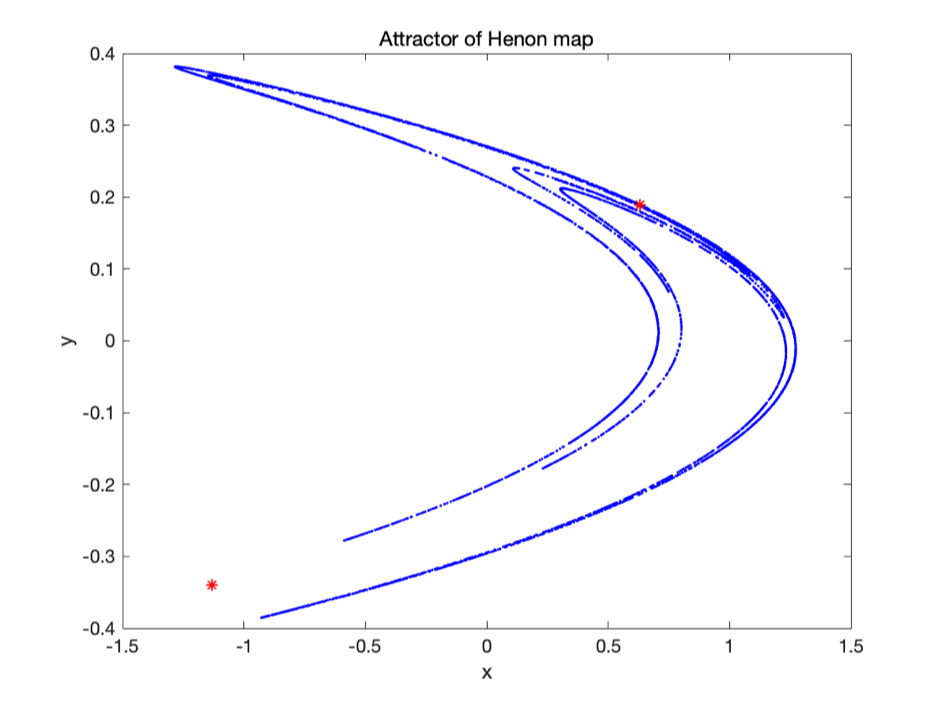
\includegraphics[scale=0.8]{henon_phase.png}
    \caption[埃农映射的吸引子和不动点]{埃农映射的吸引子和不动点($a=1.4,b=0.3$):蓝色的点表示经过多次迭代后落到的相空间中的吸引子,红色的点表示埃农映射的不动点}
    \label{fig:logi_lypn}
\end{figure}

在我们的Koopman分析中,我们在取上述参数值的情况下,通过H\'{e}non映射的迭代方程演化出一系列的数据,作为Koopman分析的源数据,以此来分析H\'{e}non映射的系统特征。


\subsection{埃农映射的Koopman算符本征函数}
在之前的章节中,我们探究了帐篷映射、Logistic映射一维映射Koopman算符的本征值与本征函数及对边界点的划分。埃农映射是一个二维映射,在二维映射中Koopman算符本征函数的计算与一维大致相同又稍有区别。且本征函数对相空间的划分又与一维情况有所不同,二维映射的动力学特征也更为复杂。在本节中,我们将探究Koopman算符的本征值与本征函数与埃农映射的动力学特征的关系及对埃农映射相空间的划分。


\subsubsection{正交完备基函数空间}
埃农映射是一个二维映射,在二维函数空间中,二维高斯基函数可以写为:
\begin{equation}
  g(x,y)=Ce^{({\dfrac{-(x-x_j)^2-(y-y_j)^2}{d_j^2}})}
\end{equation}
其中C为常系数,$(x_j,y_j)$为高斯波包的中心位置,$d_j$表示格点宽度,且我们在两个方向上并无相关性。二维傅里叶基函数可以写为:
\begin{equation}
  g(x,y)=e^{i\dfrac{\pi}{1.5}(mx+ny)},\ m,n\in\mathbb{Z}
\end{equation}
其中$m,n$表示两个方向上的频率,$\frac{\pi}{1.5}$表示在埃农映射相空间$[-1.5,1.5]\times [-1.5,1.5]$的缩放因子。我们将某一时刻的二维数据矩阵作为一组状态变量,并求得每个基函数在此状态变量下的值,作为数据矩阵,以此求得演化前矩阵$K$和演化后矩阵$L$,根据式\eqref{eq:Koop_kl1},计算Koopman算符$U$的矩阵表示及其本征值与本征函数。

图\ref{fig:henon_eig_RGFL}画出了演化格点数量$n=100\times 100$时,在二维高斯基函数、二维傅里叶基函数下埃农映射的本征值与本征函数。我们取相空间$[-1.5,1.5]\times [-1.5,1.5]$,并取前9个本征值接近1对应的本征函数。当本征函数值为复数时,我们取其实部作为我们的本征函数值。同时,我们将本征函数的实部、虚部、模、幅角在高斯基函数的本征函数图像表示在图\ref{fig:Henon_eigen_Gauss_n100m50md45_figure8}中。
\begin{figure}
    \centering
    \subfloat[高斯基函数]{
      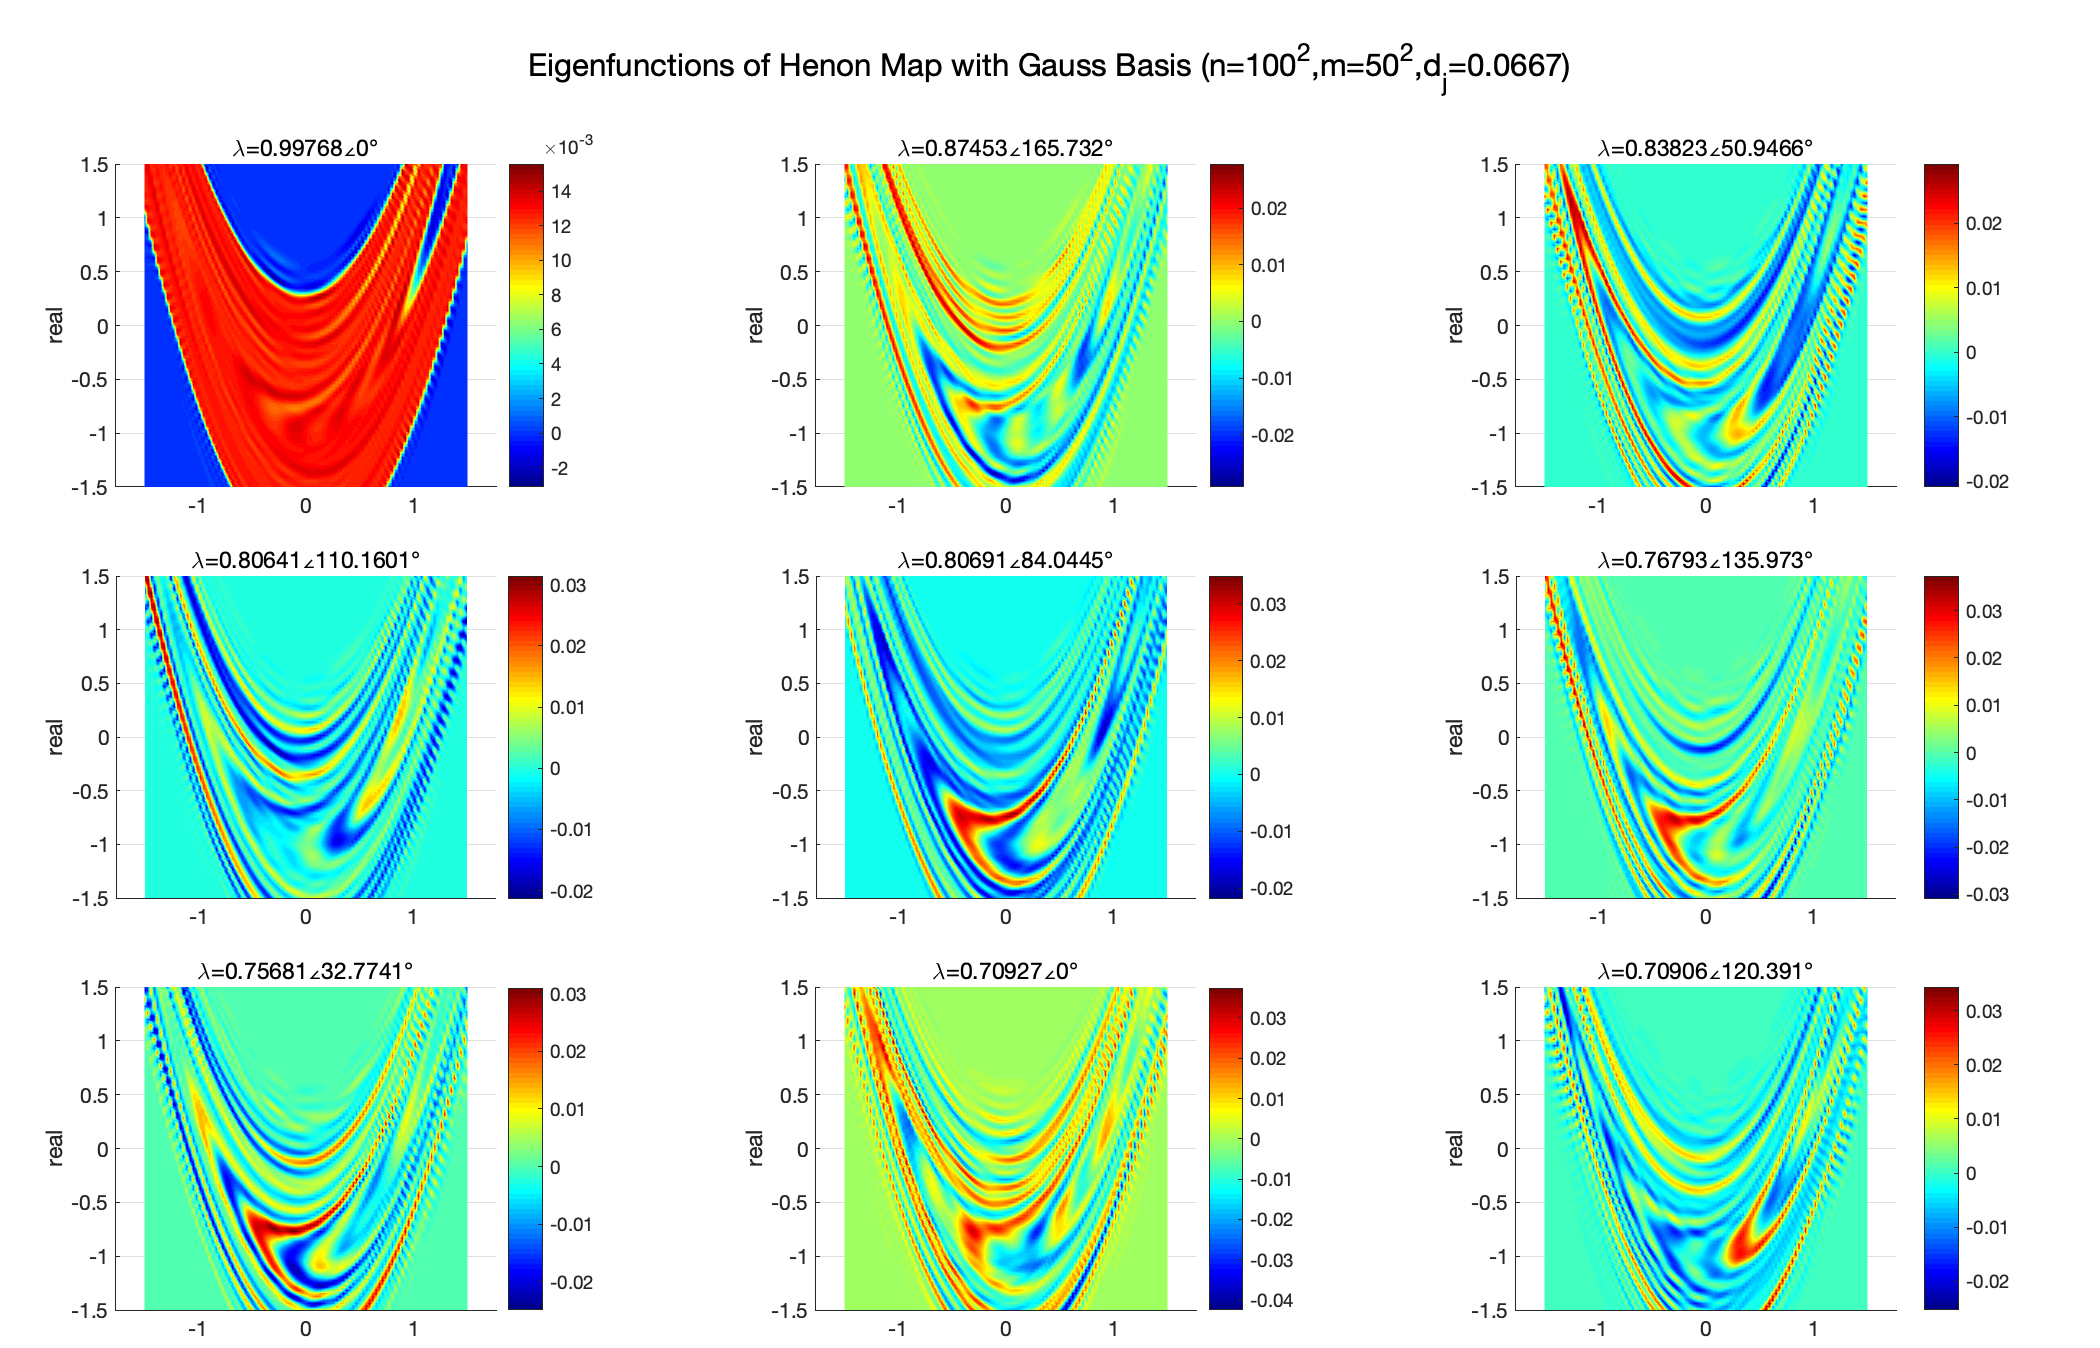
\includegraphics[scale=0.4]{henon/Henon_eigen_Gauss_n100m50md45}}
    \\
    \subfloat[傅里叶基函数]{
      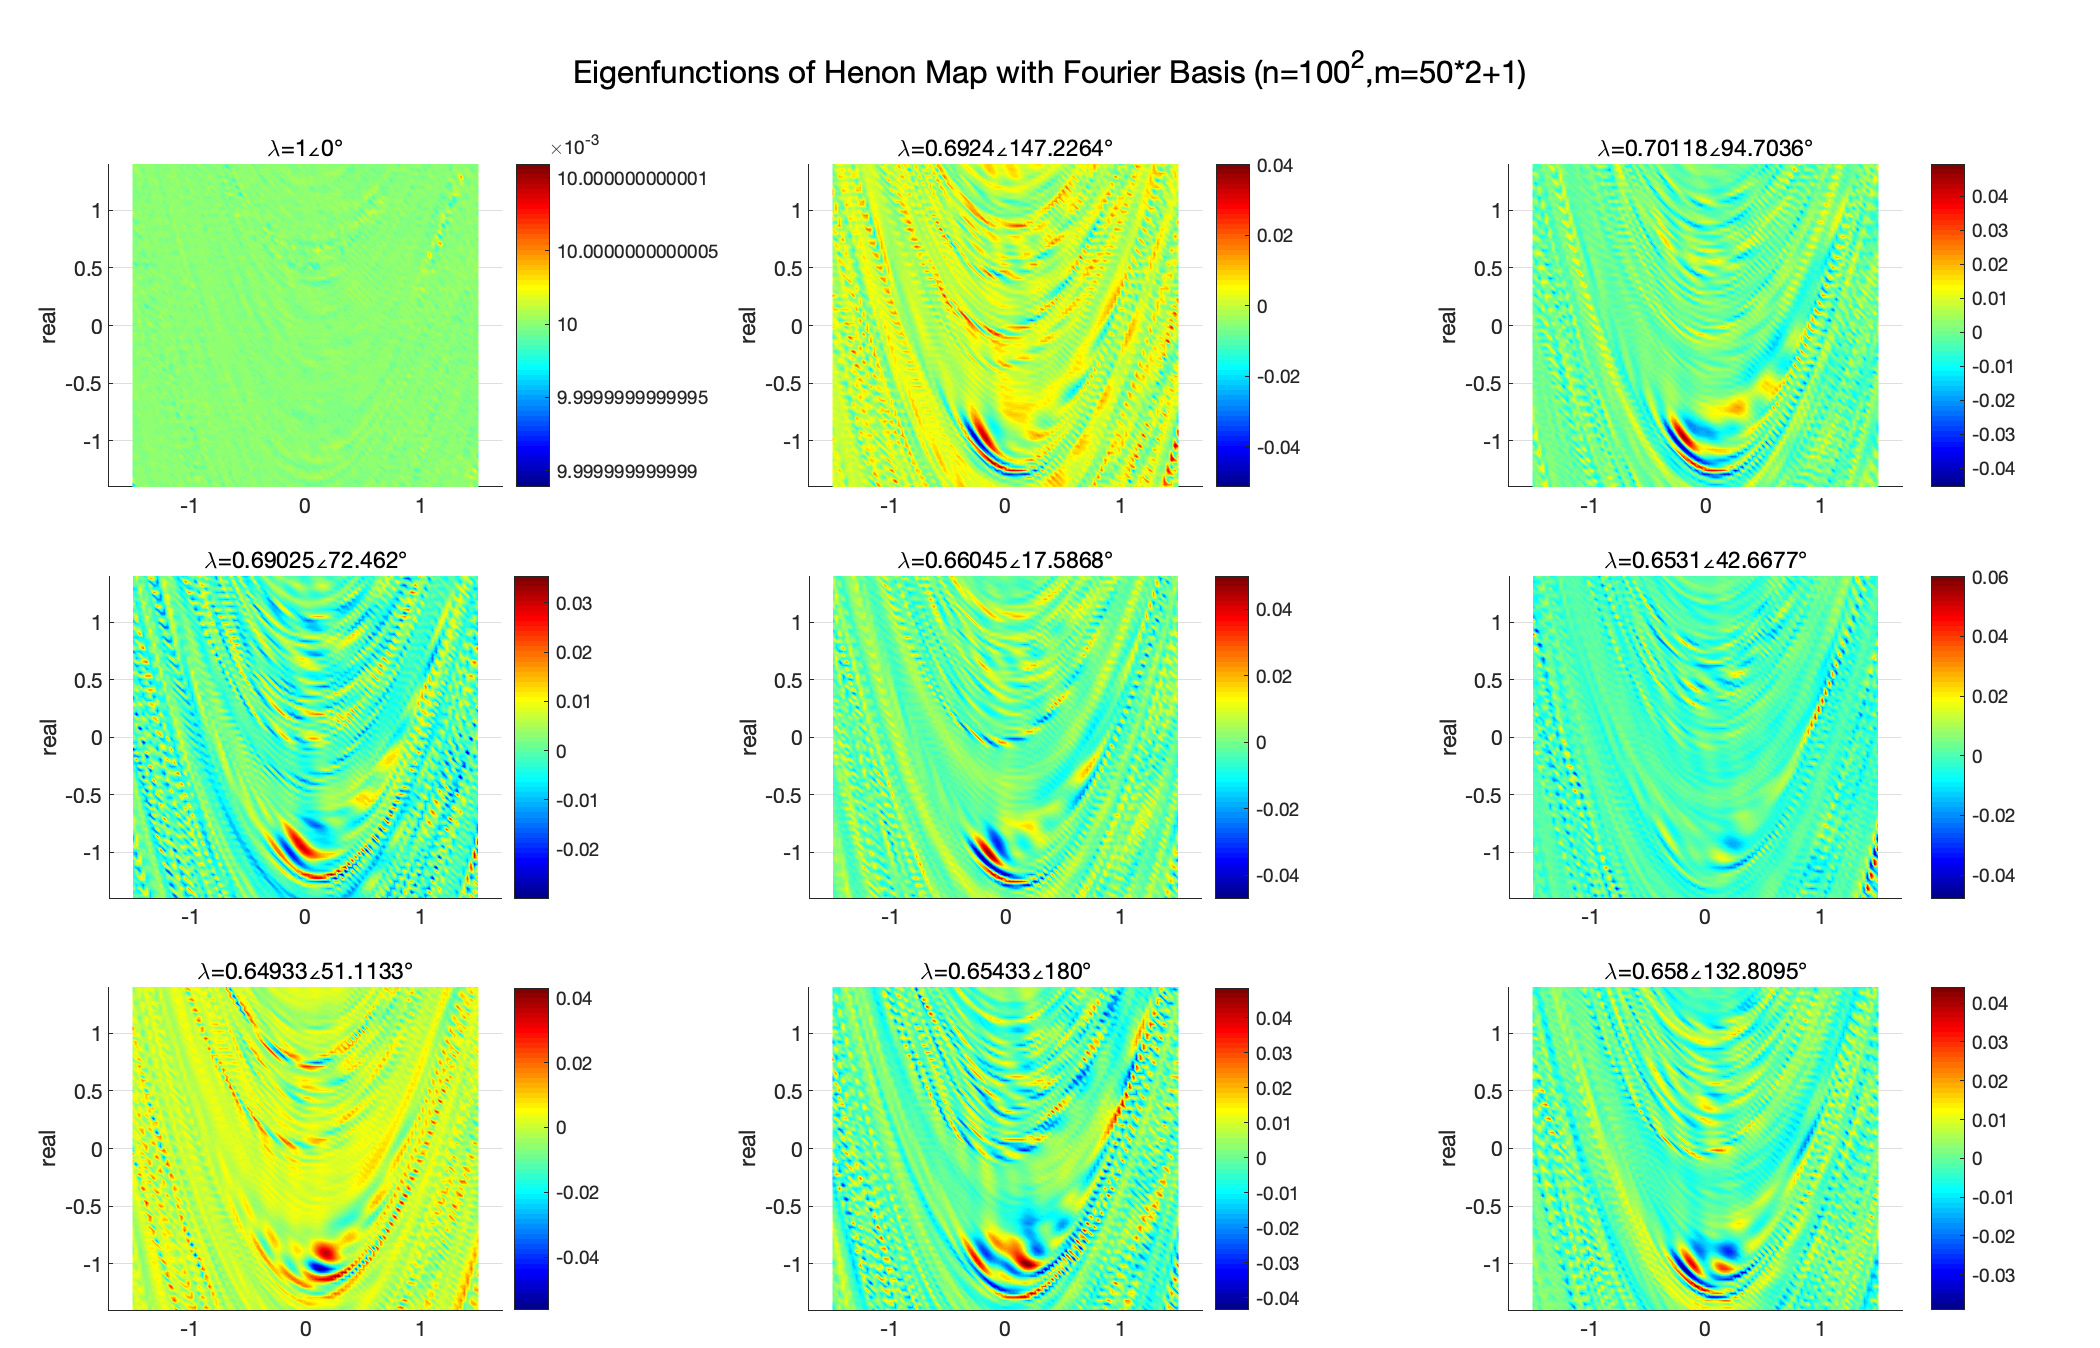
\includegraphics[scale=0.4]{henon/Henon_eigen_Fourier_n100m50}}
    \caption[埃农映射不同基函数的本征函数]{埃农映射不同基函数的本征函数}\label{fig:henon_eig_RGFL}
\end{figure}
\begin{figure}
  \centering
  \subfloat{
    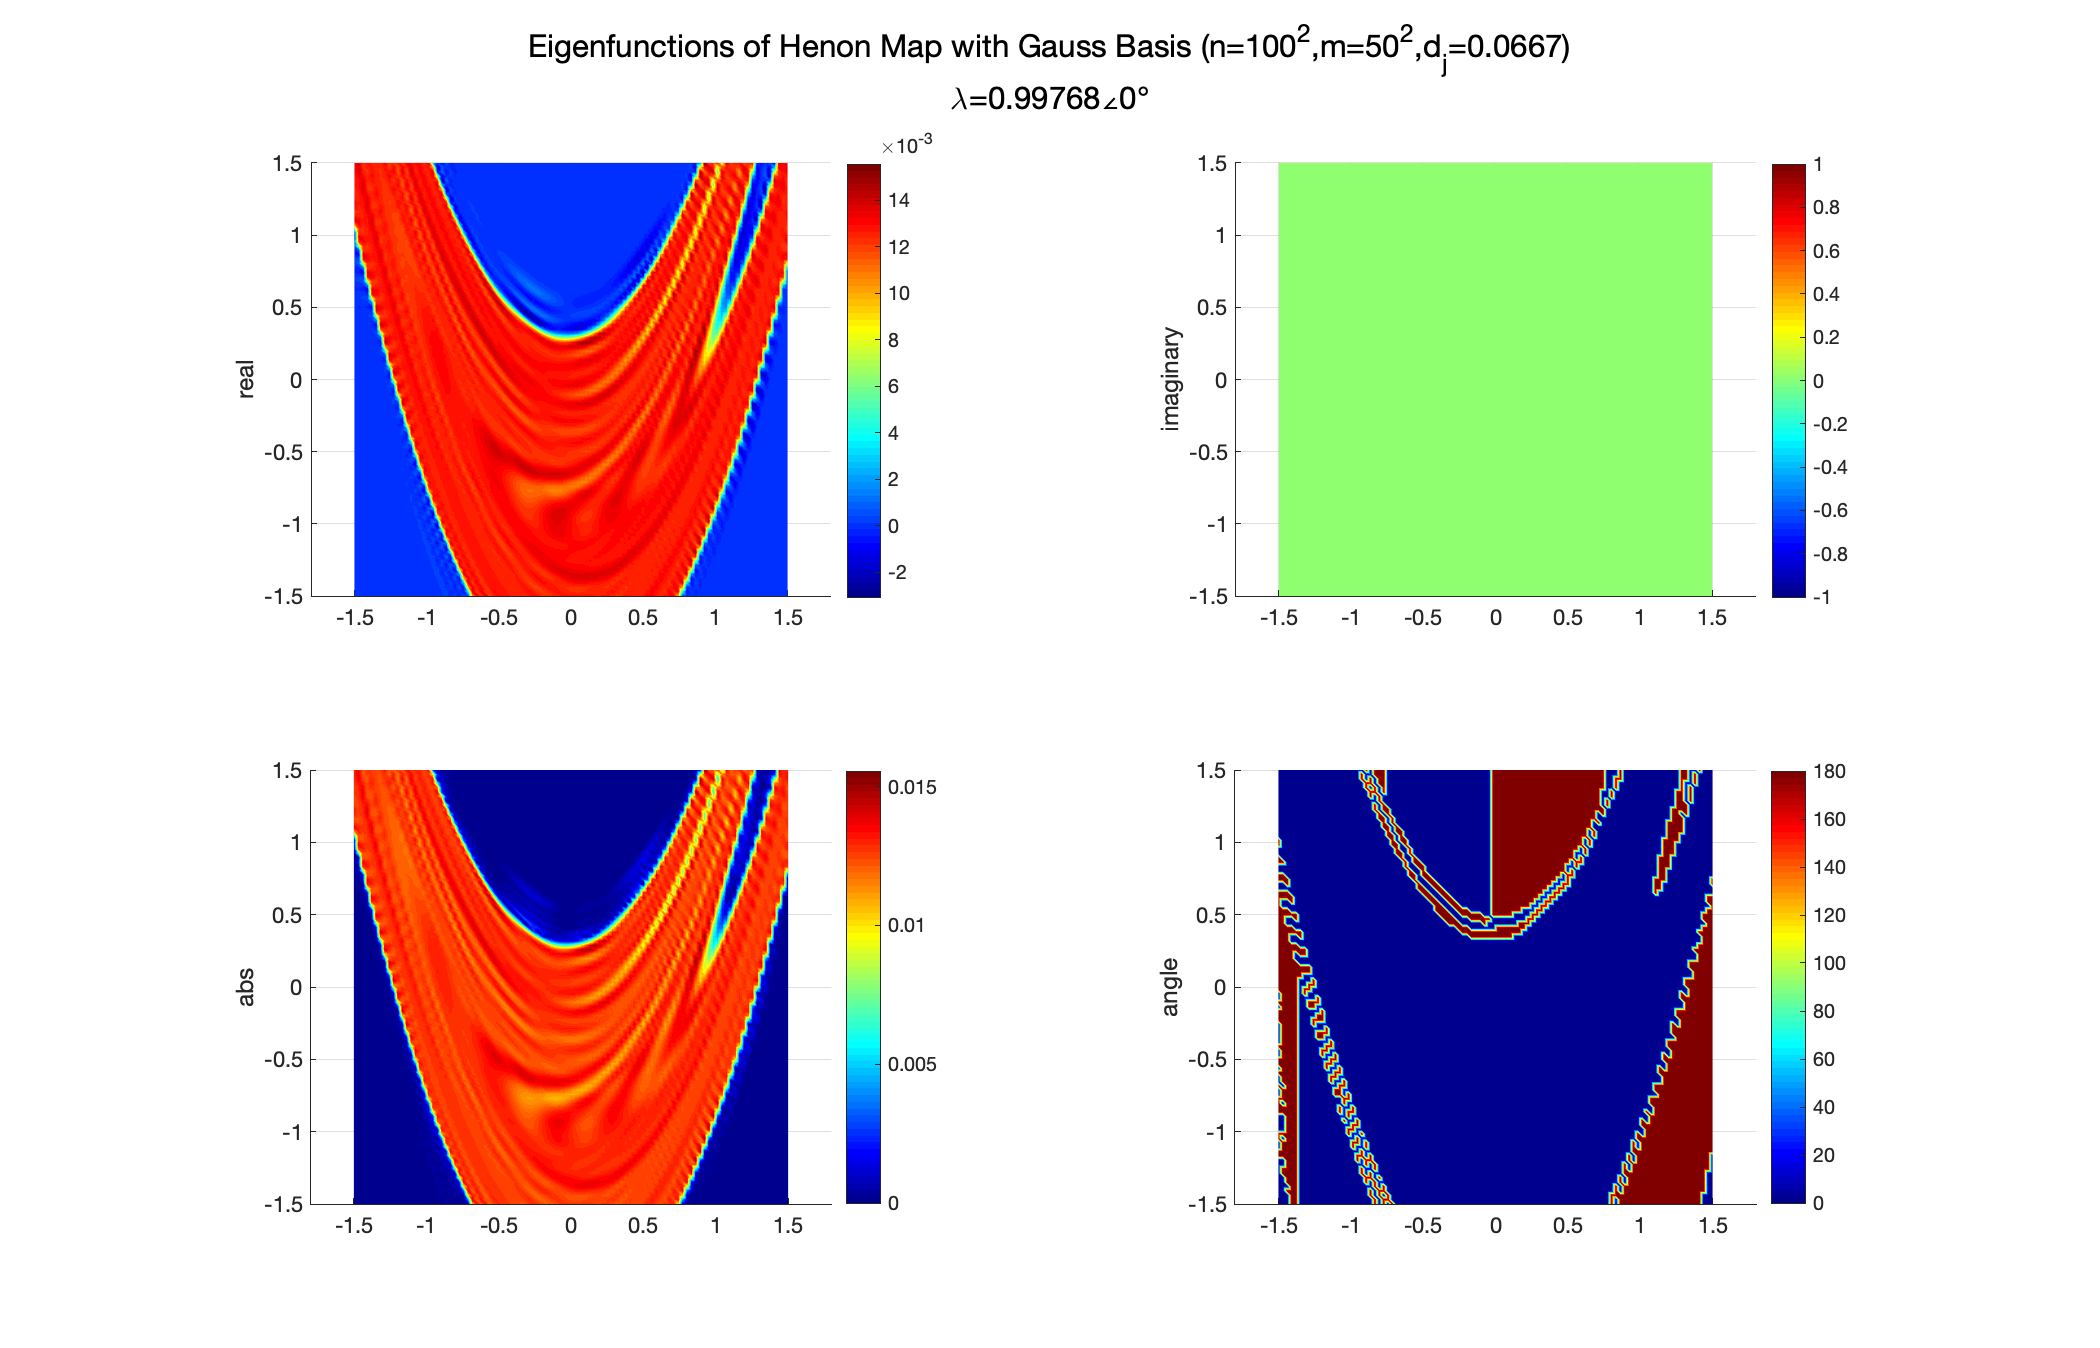
\includegraphics[scale=0.2]{henon/Henon_eigen_Gauss_n100m50md45_figure1}}
  \subfloat{
    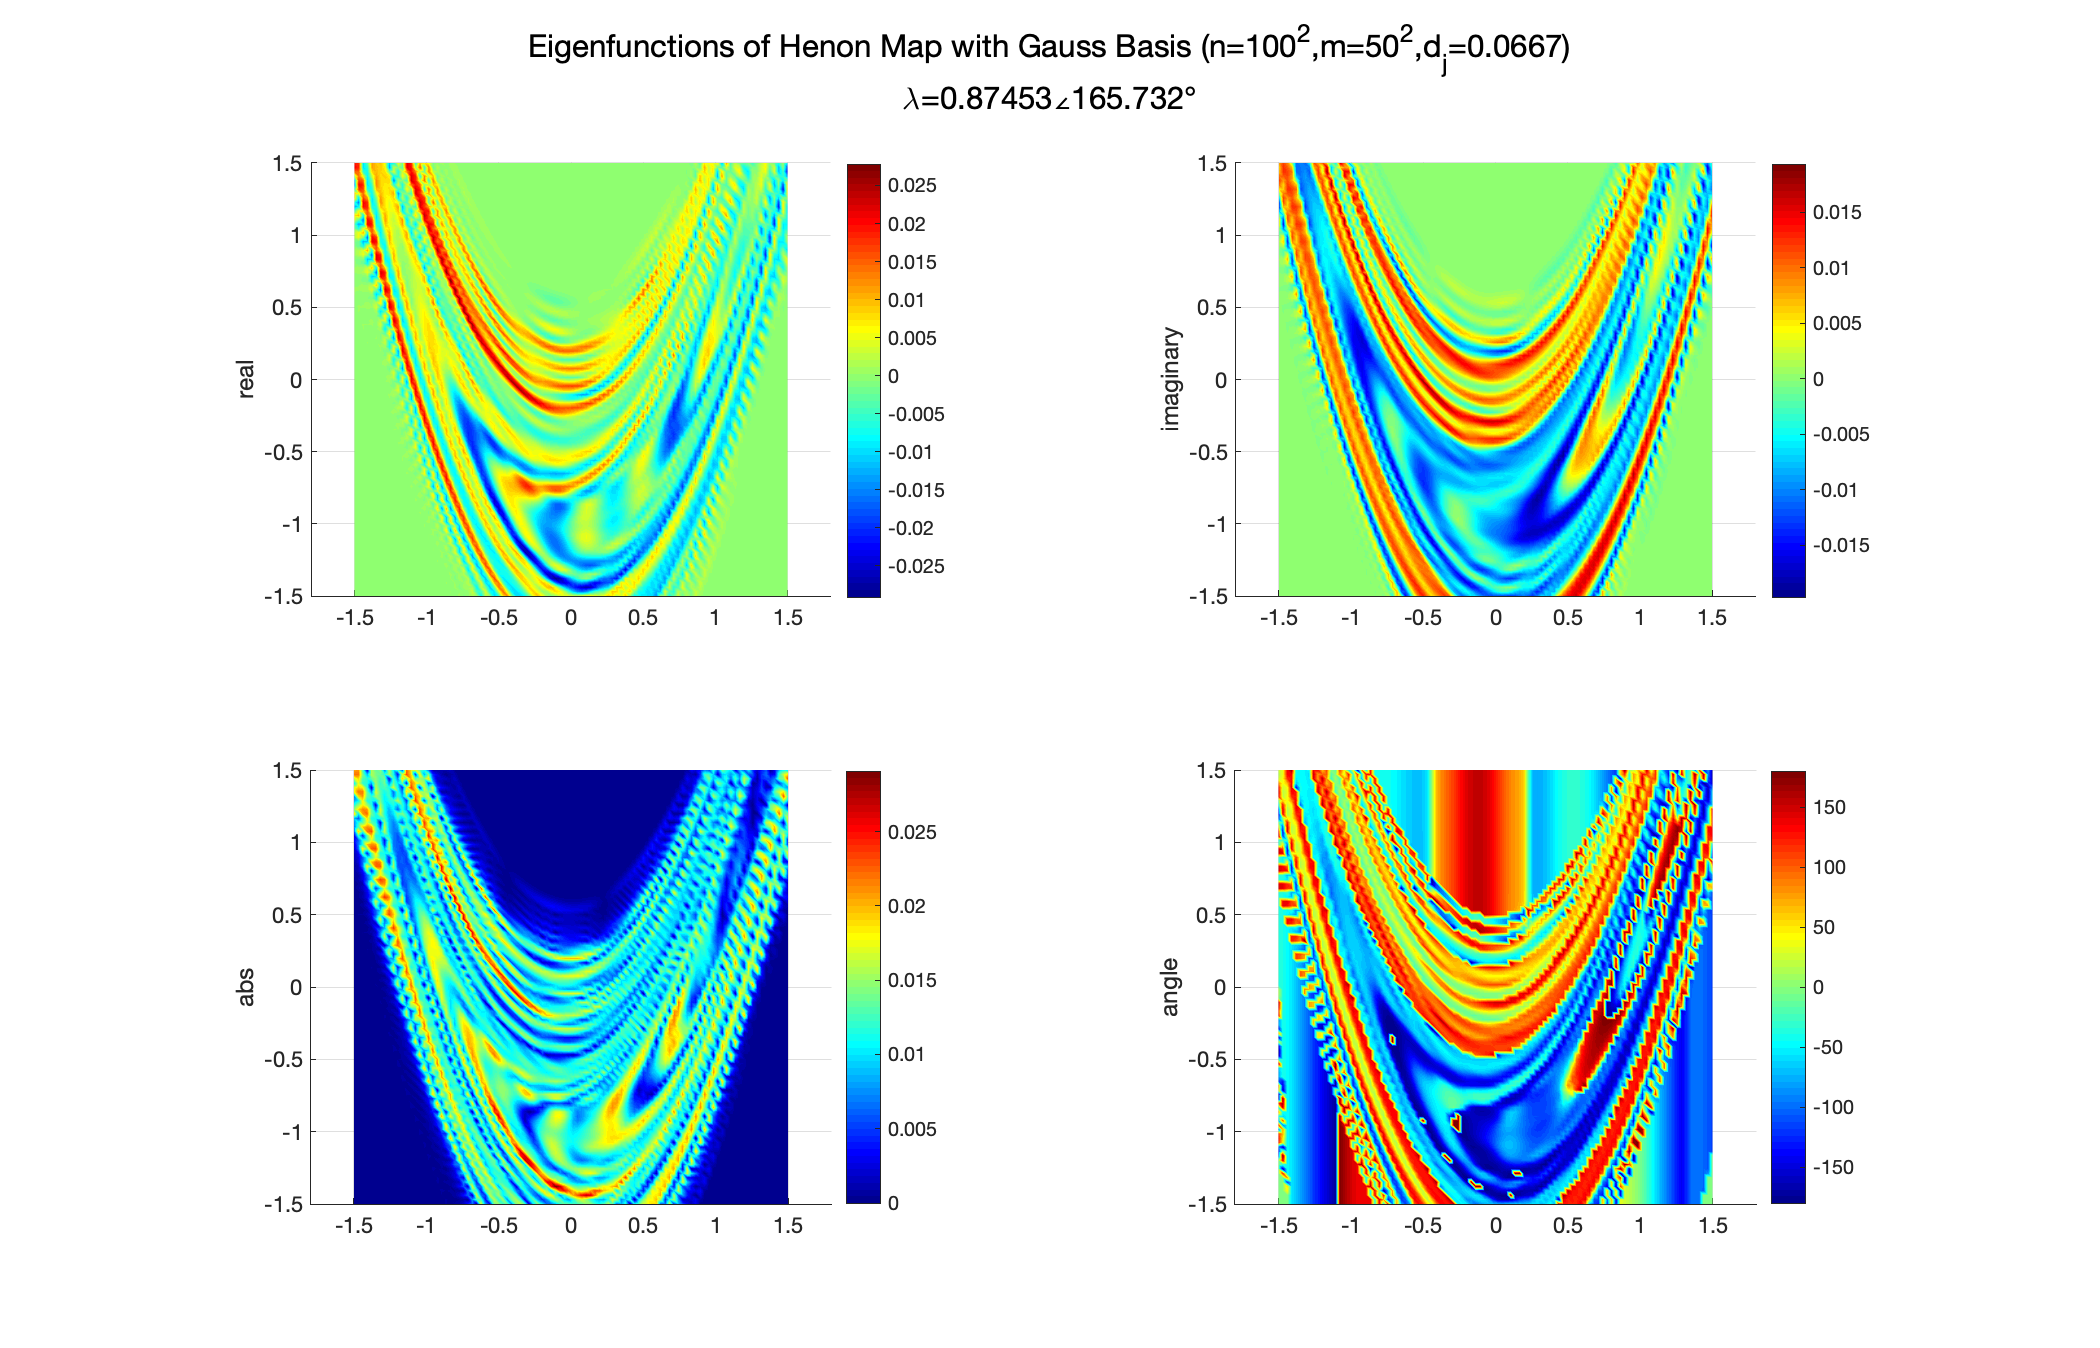
\includegraphics[scale=0.2]{henon/Henon_eigen_Gauss_n100m50md45_figure2}}
  \\
  \subfloat{
    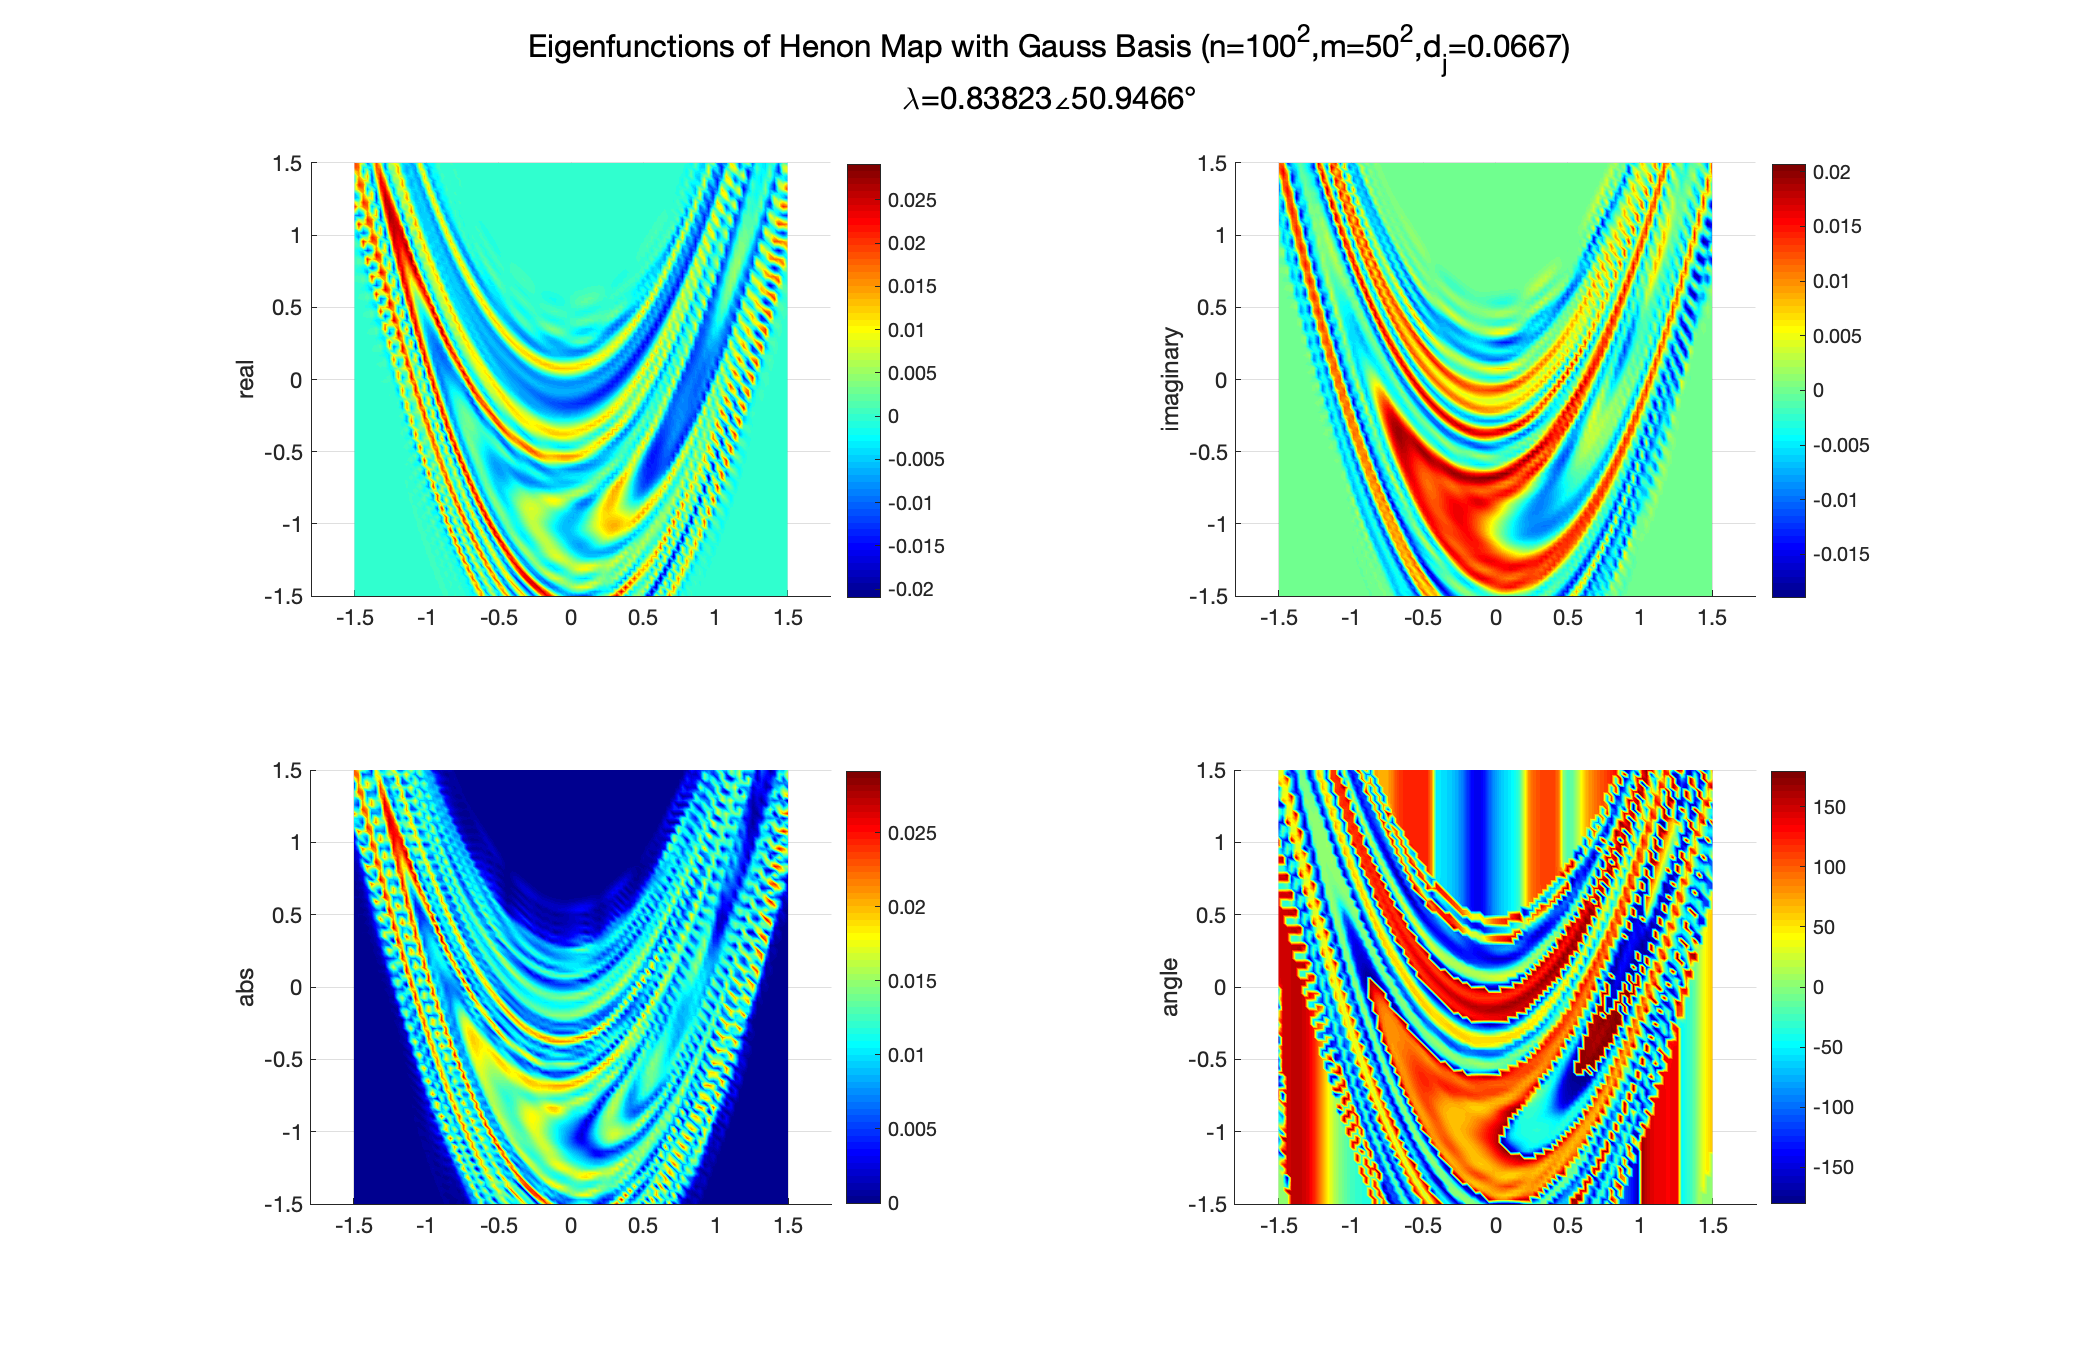
\includegraphics[scale=0.2]{henon/Henon_eigen_Gauss_n100m50md45_figure3}}
  \subfloat{
    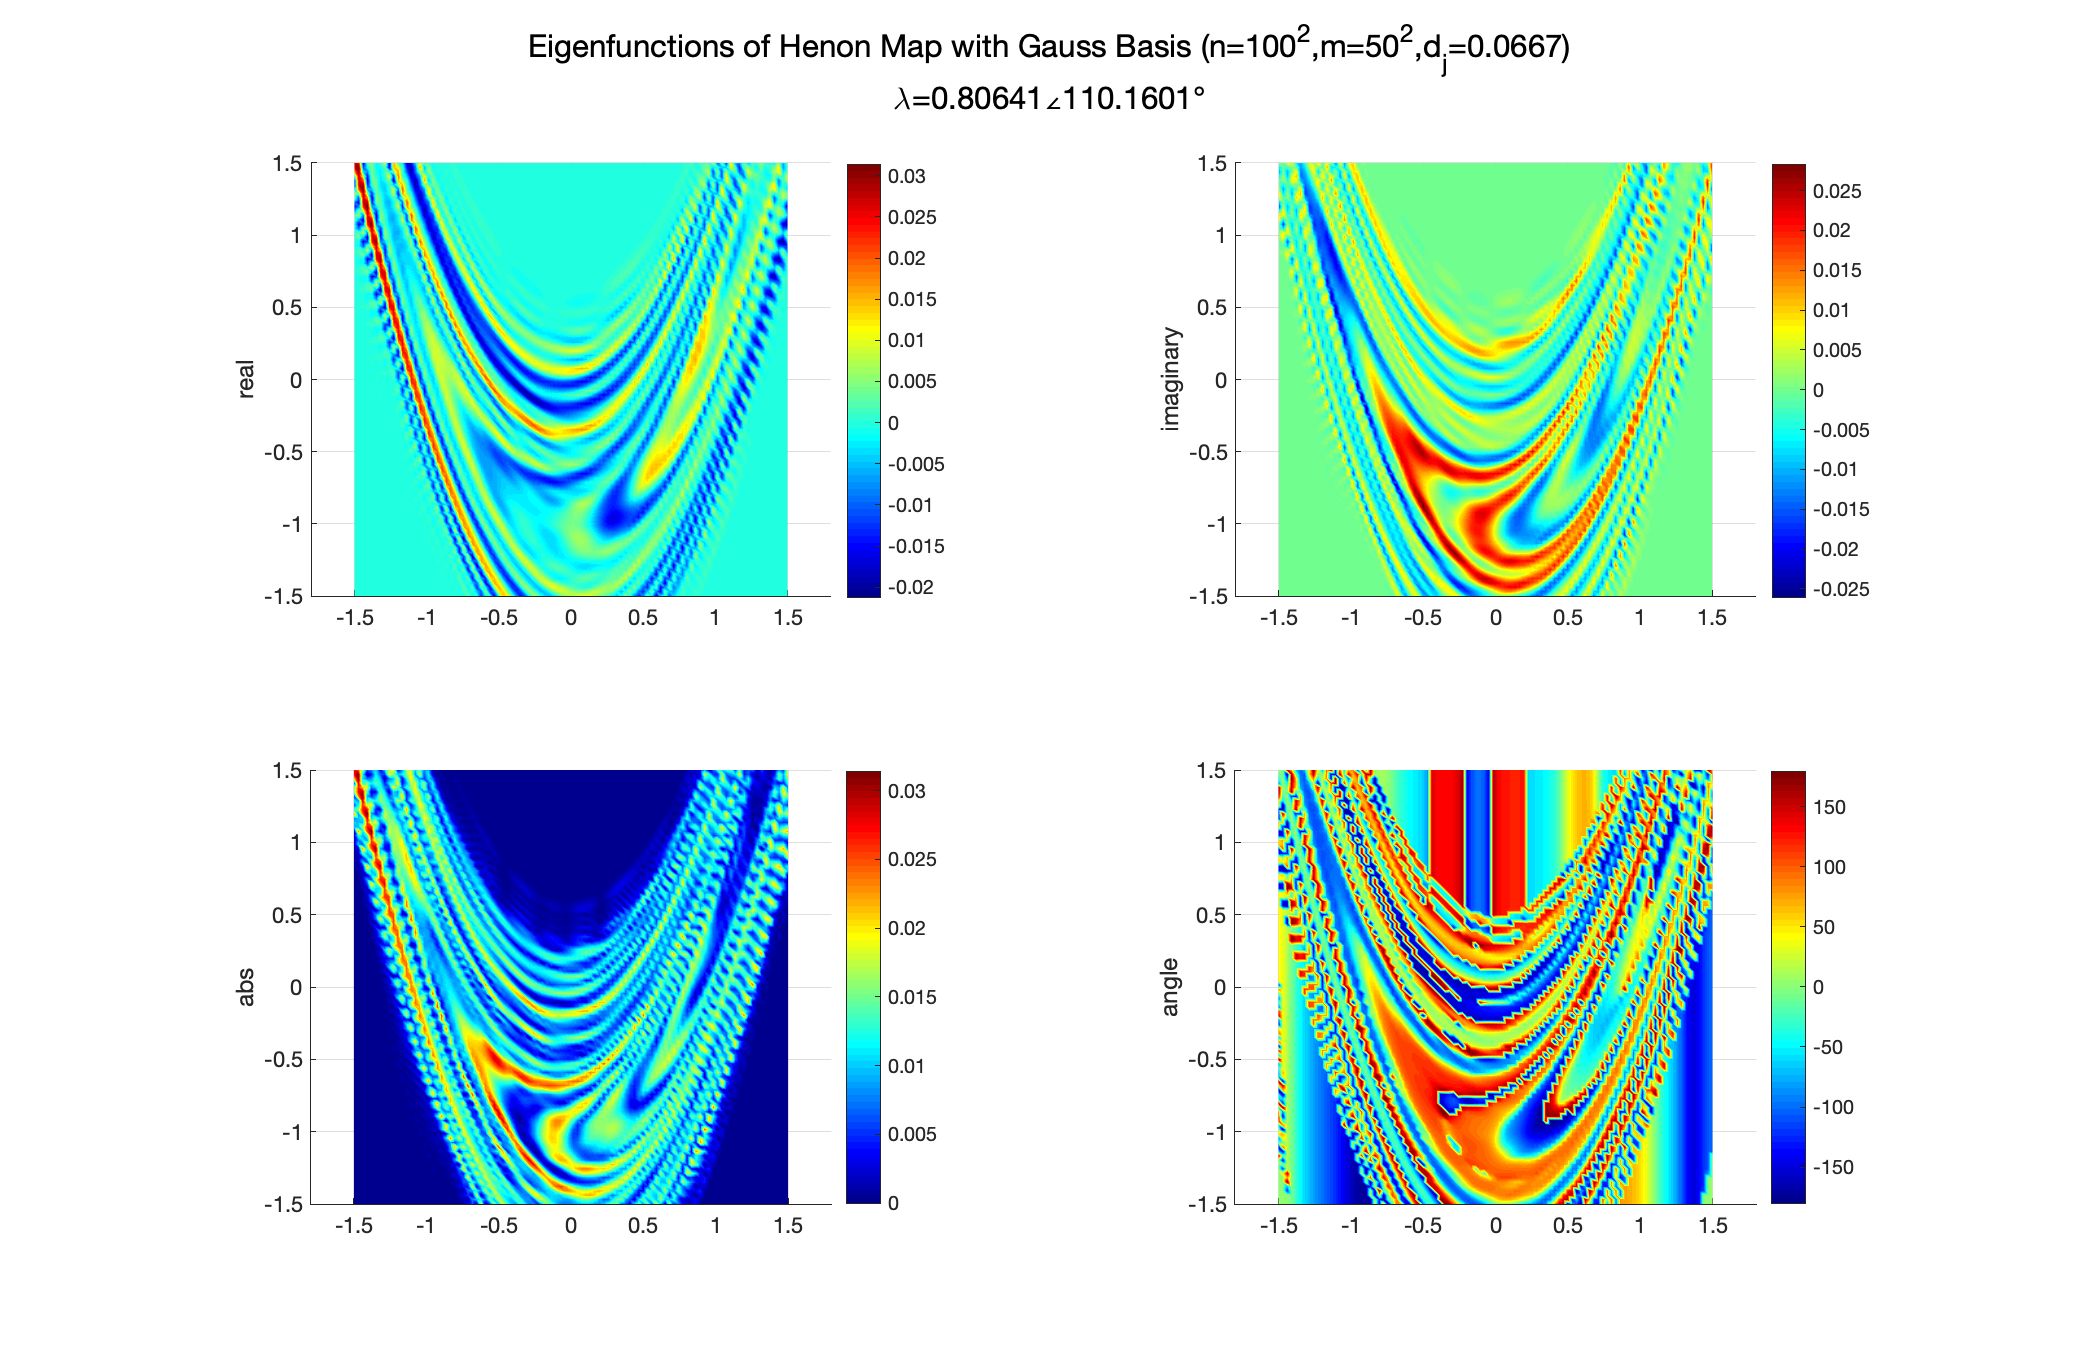
\includegraphics[scale=0.2]{henon/Henon_eigen_Gauss_n100m50md45_figure4}}
  \\
  \subfloat{
    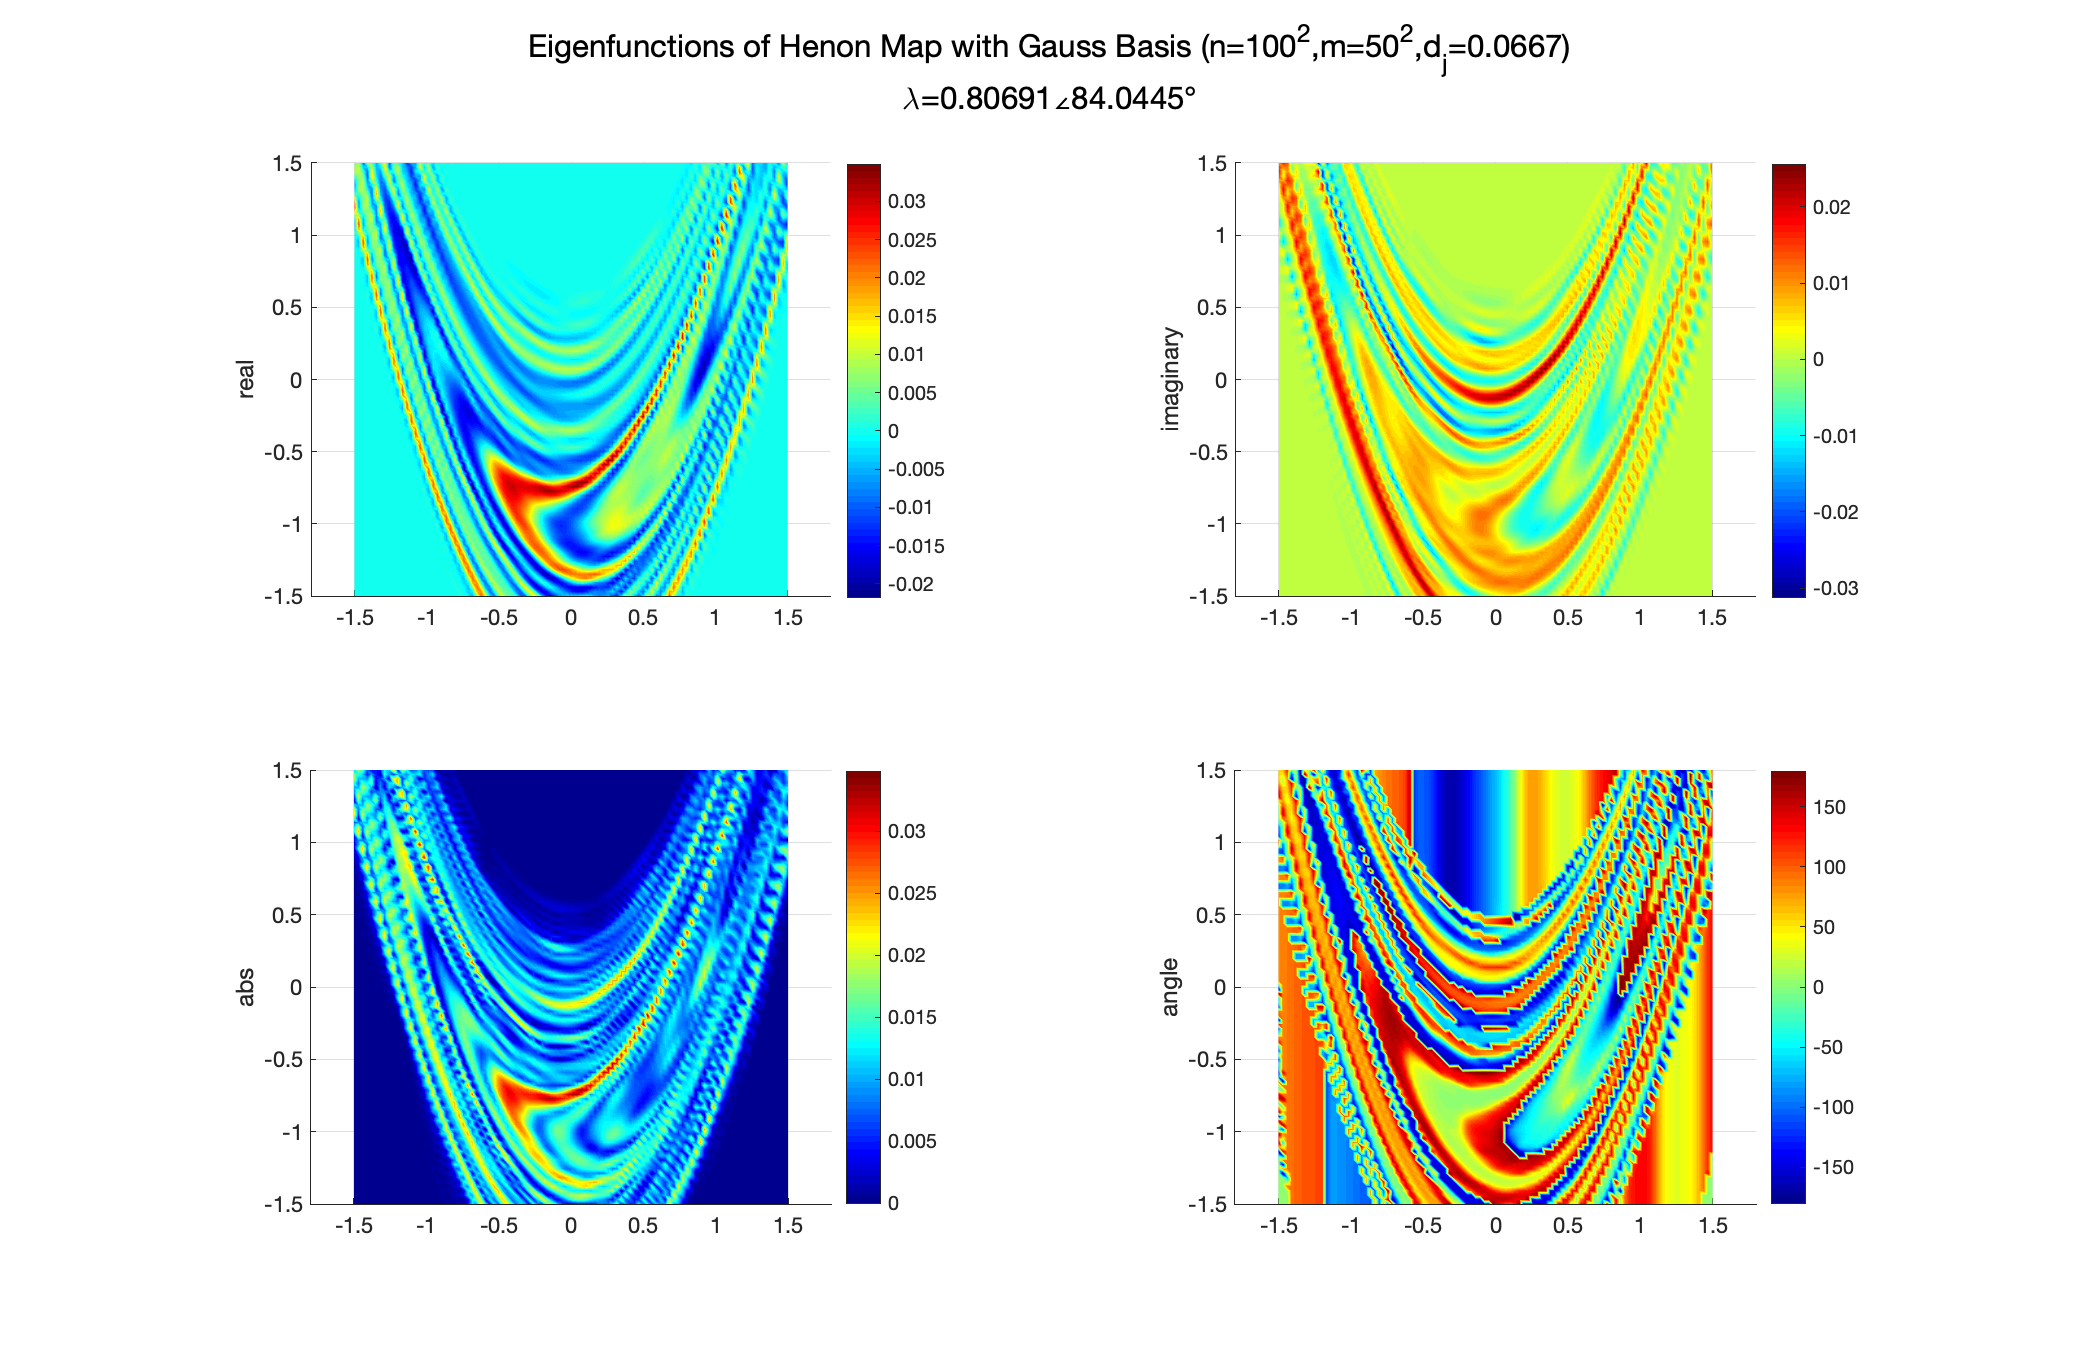
\includegraphics[scale=0.2]{henon/Henon_eigen_Gauss_n100m50md45_figure5}}
  \subfloat{
    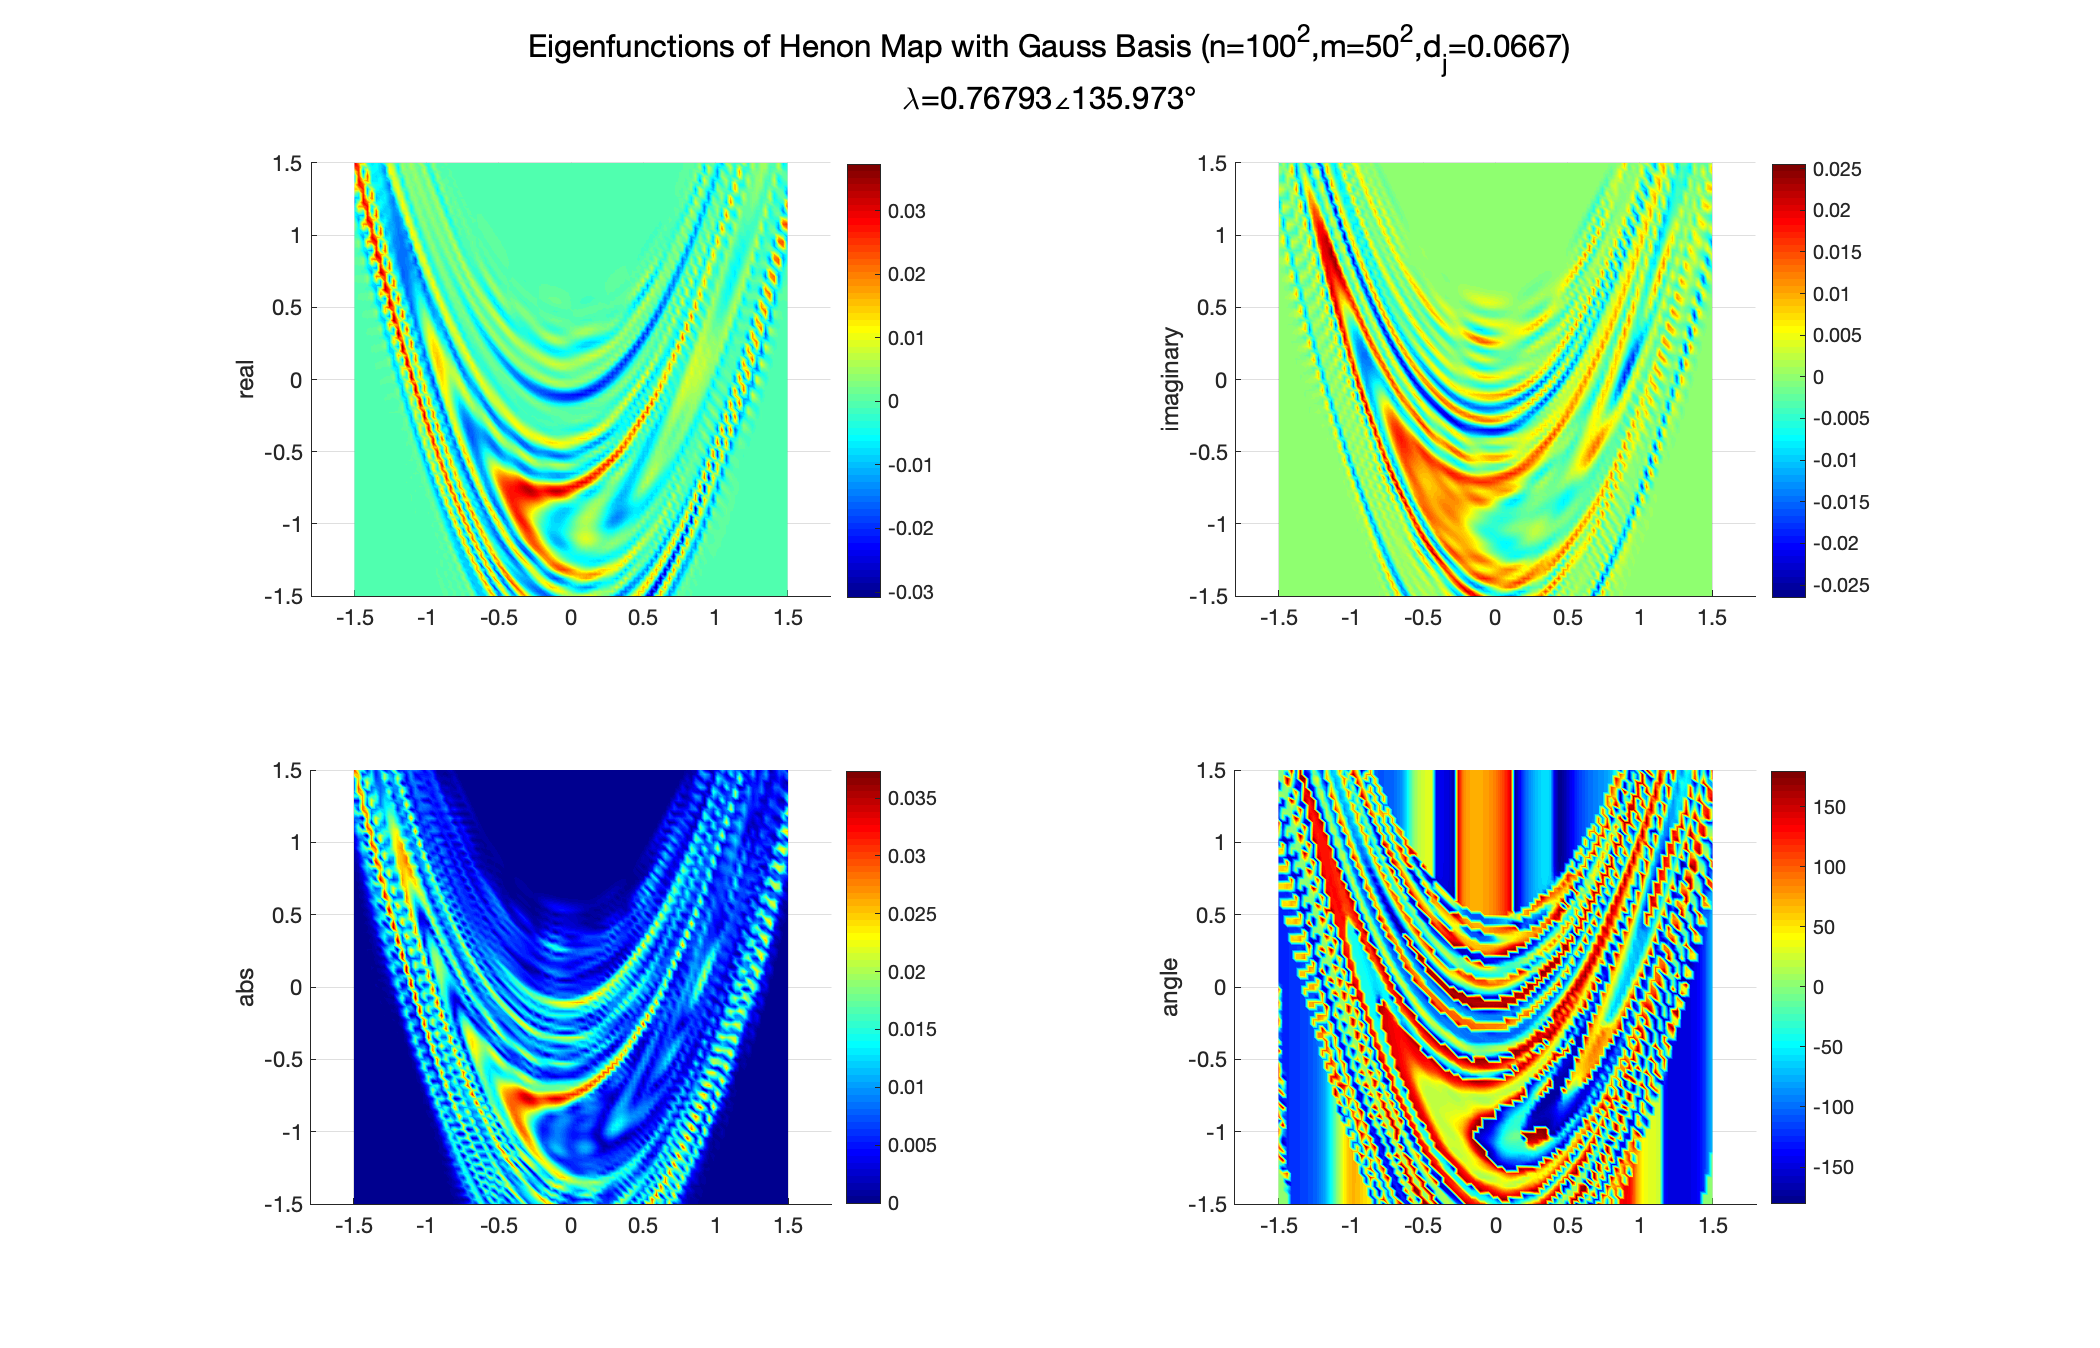
\includegraphics[scale=0.2]{henon/Henon_eigen_Gauss_n100m50md45_figure6}}
  \\
  \subfloat{
    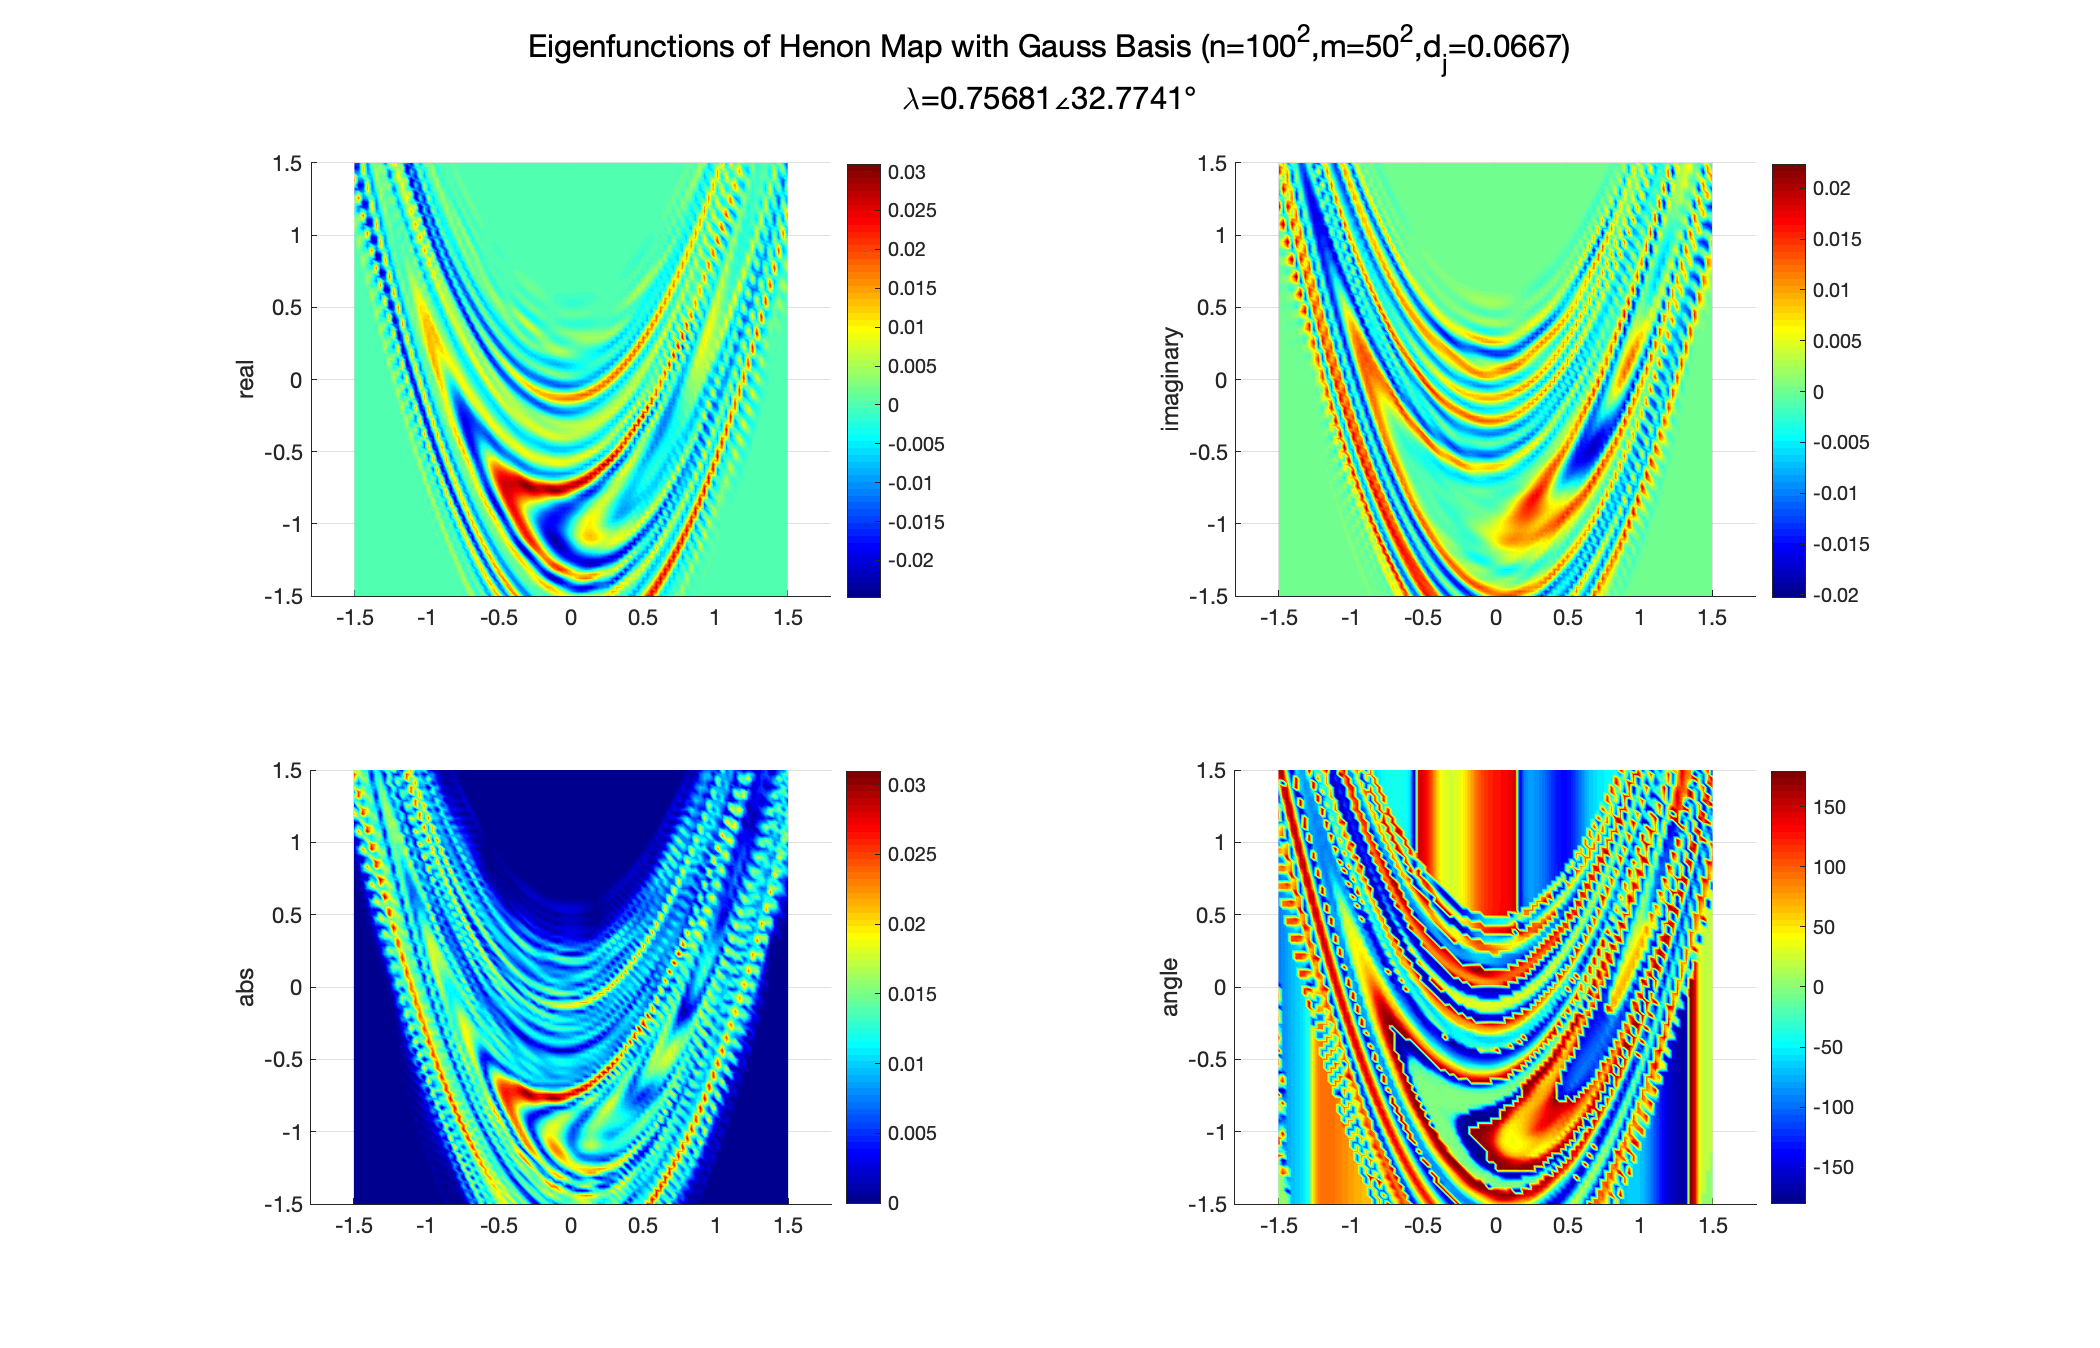
\includegraphics[scale=0.2]{henon/Henon_eigen_Gauss_n100m50md45_figure7}}
  \subfloat{
    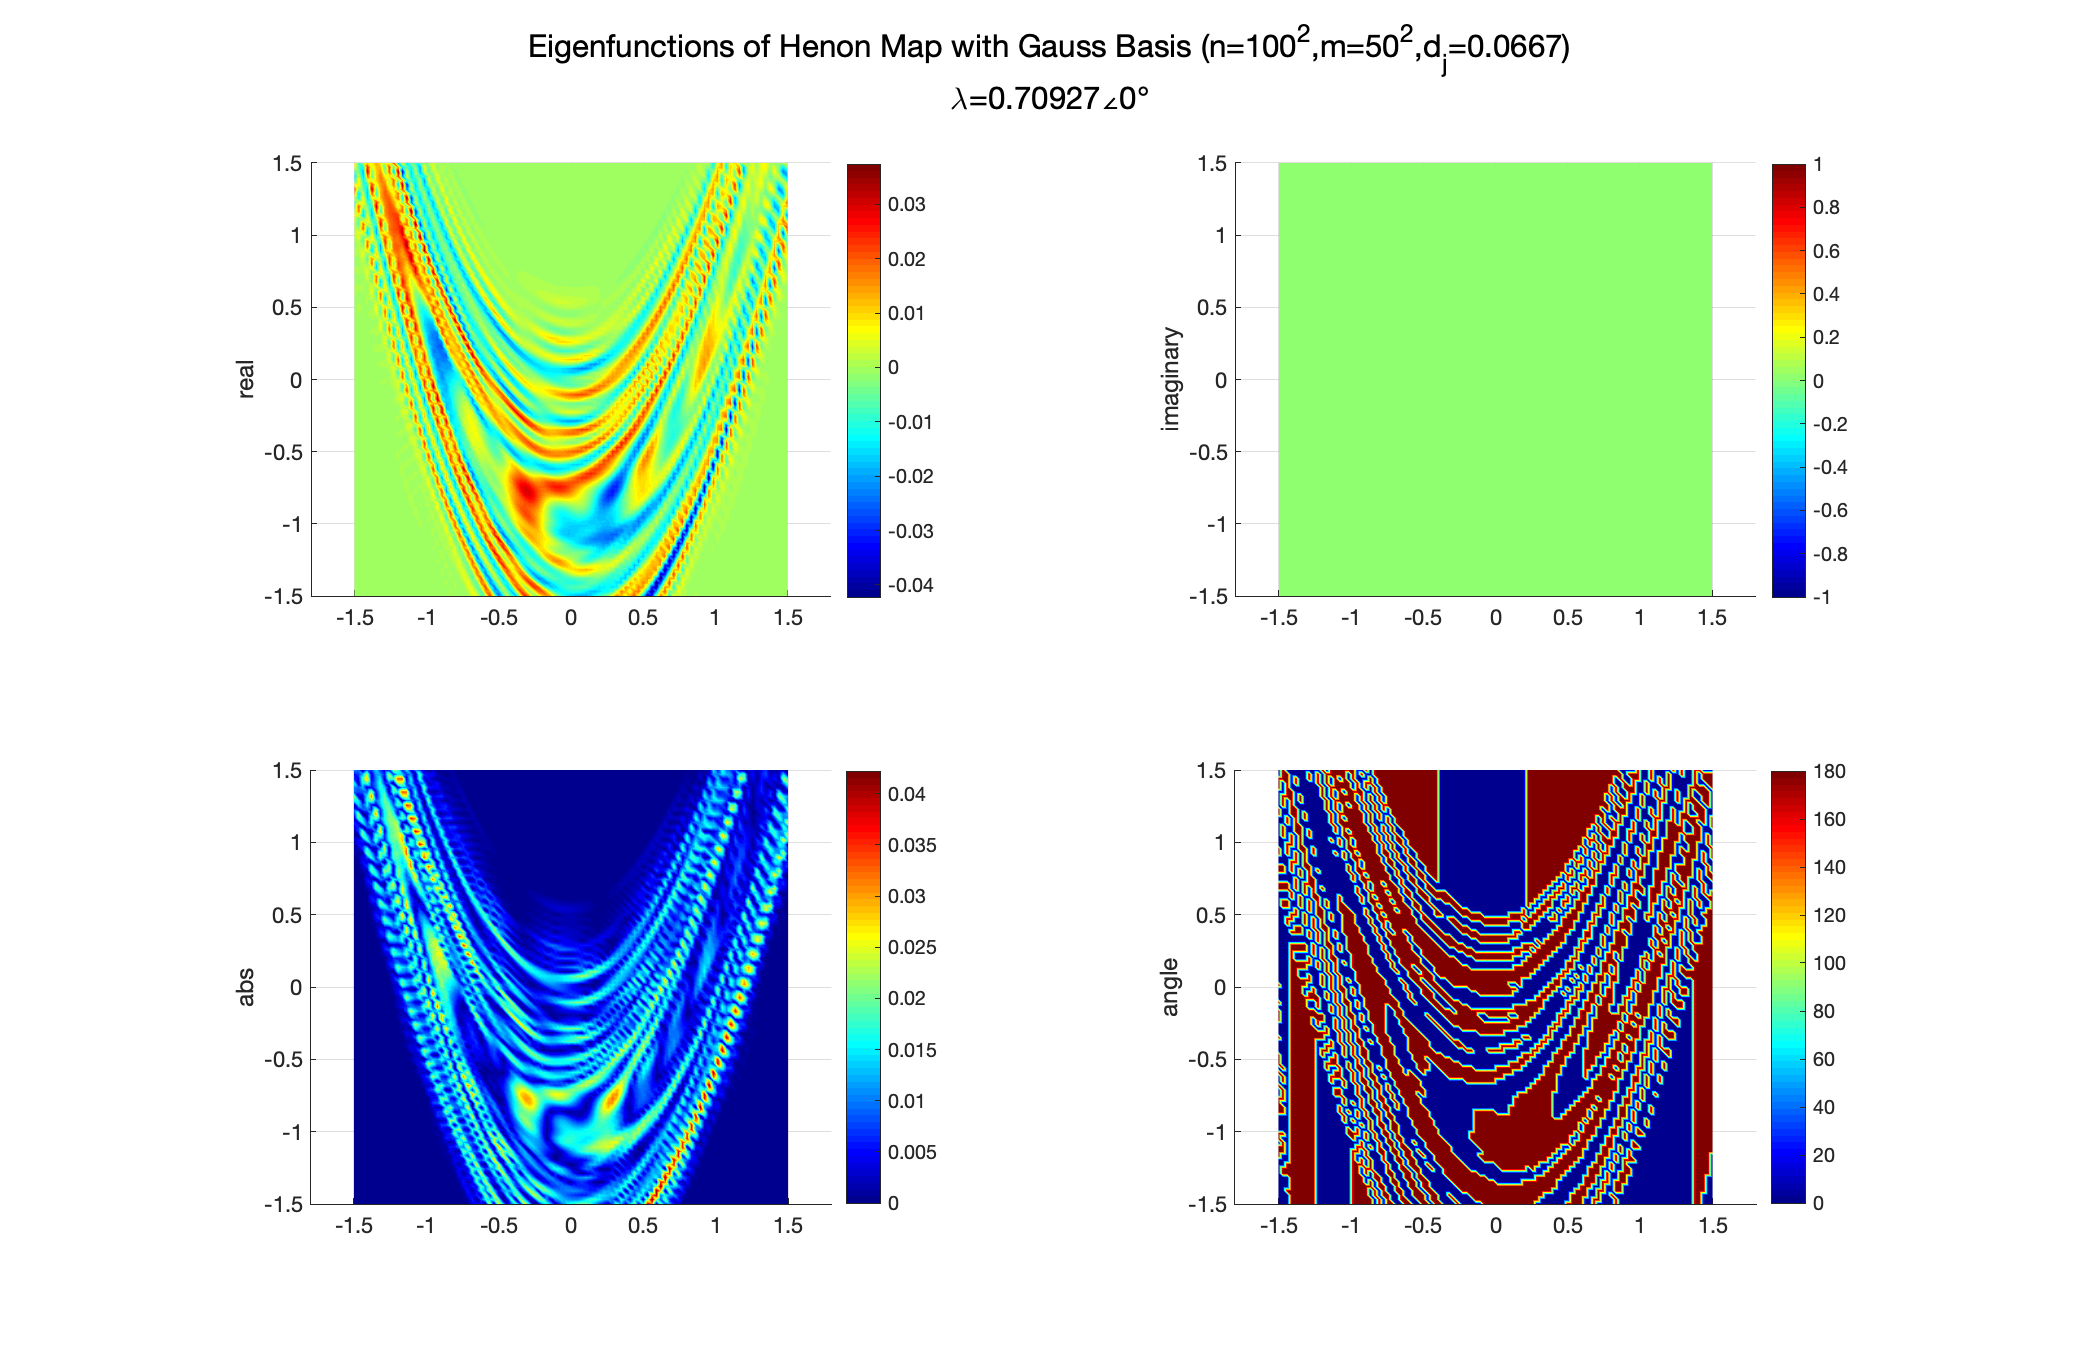
\includegraphics[scale=0.2]{henon/Henon_eigen_Gauss_n100m50md45_figure8}}
  \\
  \caption[埃农映射不同本征值的本征函数]{埃农映射不同本征值的本征函数($n=100^2$,$m=50^2,d_j=\frac{3}{45}$):每个子图中又分为四个小图,分别表示本征函数的实部、虚部、模、幅角}\label{fig:Henon_eigen_Gauss_n100m50md45_figure8}
\end{figure}

从图\ref{fig:henon_eig_RGFL}中,我们发现在高斯基函数和傅里叶基函数两种基函数下,本征函数的图像有着固定的差别:高斯基函数本征函数图像的连续性与平滑性较好,傅里叶基函数本征函数图像存在许多断断续续的极值点。但我们似乎可以观察到其二者的轮廓有着相似的结构。在之前的讨论中,我们提到,本征函数总是在选取的基函数空间内,即从数学上每个本征函数都由所有的基函数线性组合而成。因此我们的本征函数只是在此函数空间上的一个近似(或者说是函数几何空间从高维到低维的投影),因此基函数的选取会影响本征函数空间,因此我们对基函数的选取亦至关重要。为了能更好的划分出相空间,我们应尽量体现出不同基函数的作用,以此对相空间进行划分。显然,二维高斯基函数的局部性更好,而二维傅里叶基函数在其相空间属于全局函数,不利于对相空间划分的表示。为此,在我们后面的讨论中,我们将选取高斯基函数来讨论Koopman算符的本征函数。

在图\ref{fig:henon_eig_RGFL}中,每个子图中都包含4个不同的本征值及其对应的4个本征函数图像,且其中包含一个$\lambda\approx 1$的本征值,在之前的讨论中,我们认为本征值接近1的本征函数反映了相空间中一条随时间演化不变的轨道。而我们在矩形窗基函数和傅里叶基函数中也确实看到了这样的常函数轨道。而其他的本征值则不趋于1,这也可以从我们对函数空间选取的不够完备去考虑:我们不可能选取一个完全完备的函数空间,我们的本征函数只是在此函数空间的一个近似。

图\ref{fig:henon_eig_RGFL}中画出了$m=4$时的本征函数,当$m$取不同值时,如$m$越来越大时,意味着我们的函数空间的维度更高,可以描述的本征函数的维度也就越高,则对于局部函数如高斯函数而言,我们描述本征函数的精细度就更高,于是我们可以提高基函数数量$m$的大小,用以描述更精细的本征函数。

在后续的讨论中,我们会在埃农映射的吸引子域中作Koopman算符的本征函数。为了更好的对比,我们将吸引子域中埃农映射在二维高斯基函数中的本征函数图像作出,以作对比。

图\ref{fig:Henon_eigen_Gauss_attr_n6245m50md45}画出了当吸引子演化格点数量$n=6245$,高斯基函数数量$m=50\times 50=2500$时的本征函数图像,在二维平面图中不易观察其本征函数值之间的关系,为此我们在三维中作图,并将z轴的高度作为本征函数值的大小,并调整了视角,使得我们可以更清晰的观察本征函数值。
\begin{figure}
  \centering
  \subfloat[俯视图]{
    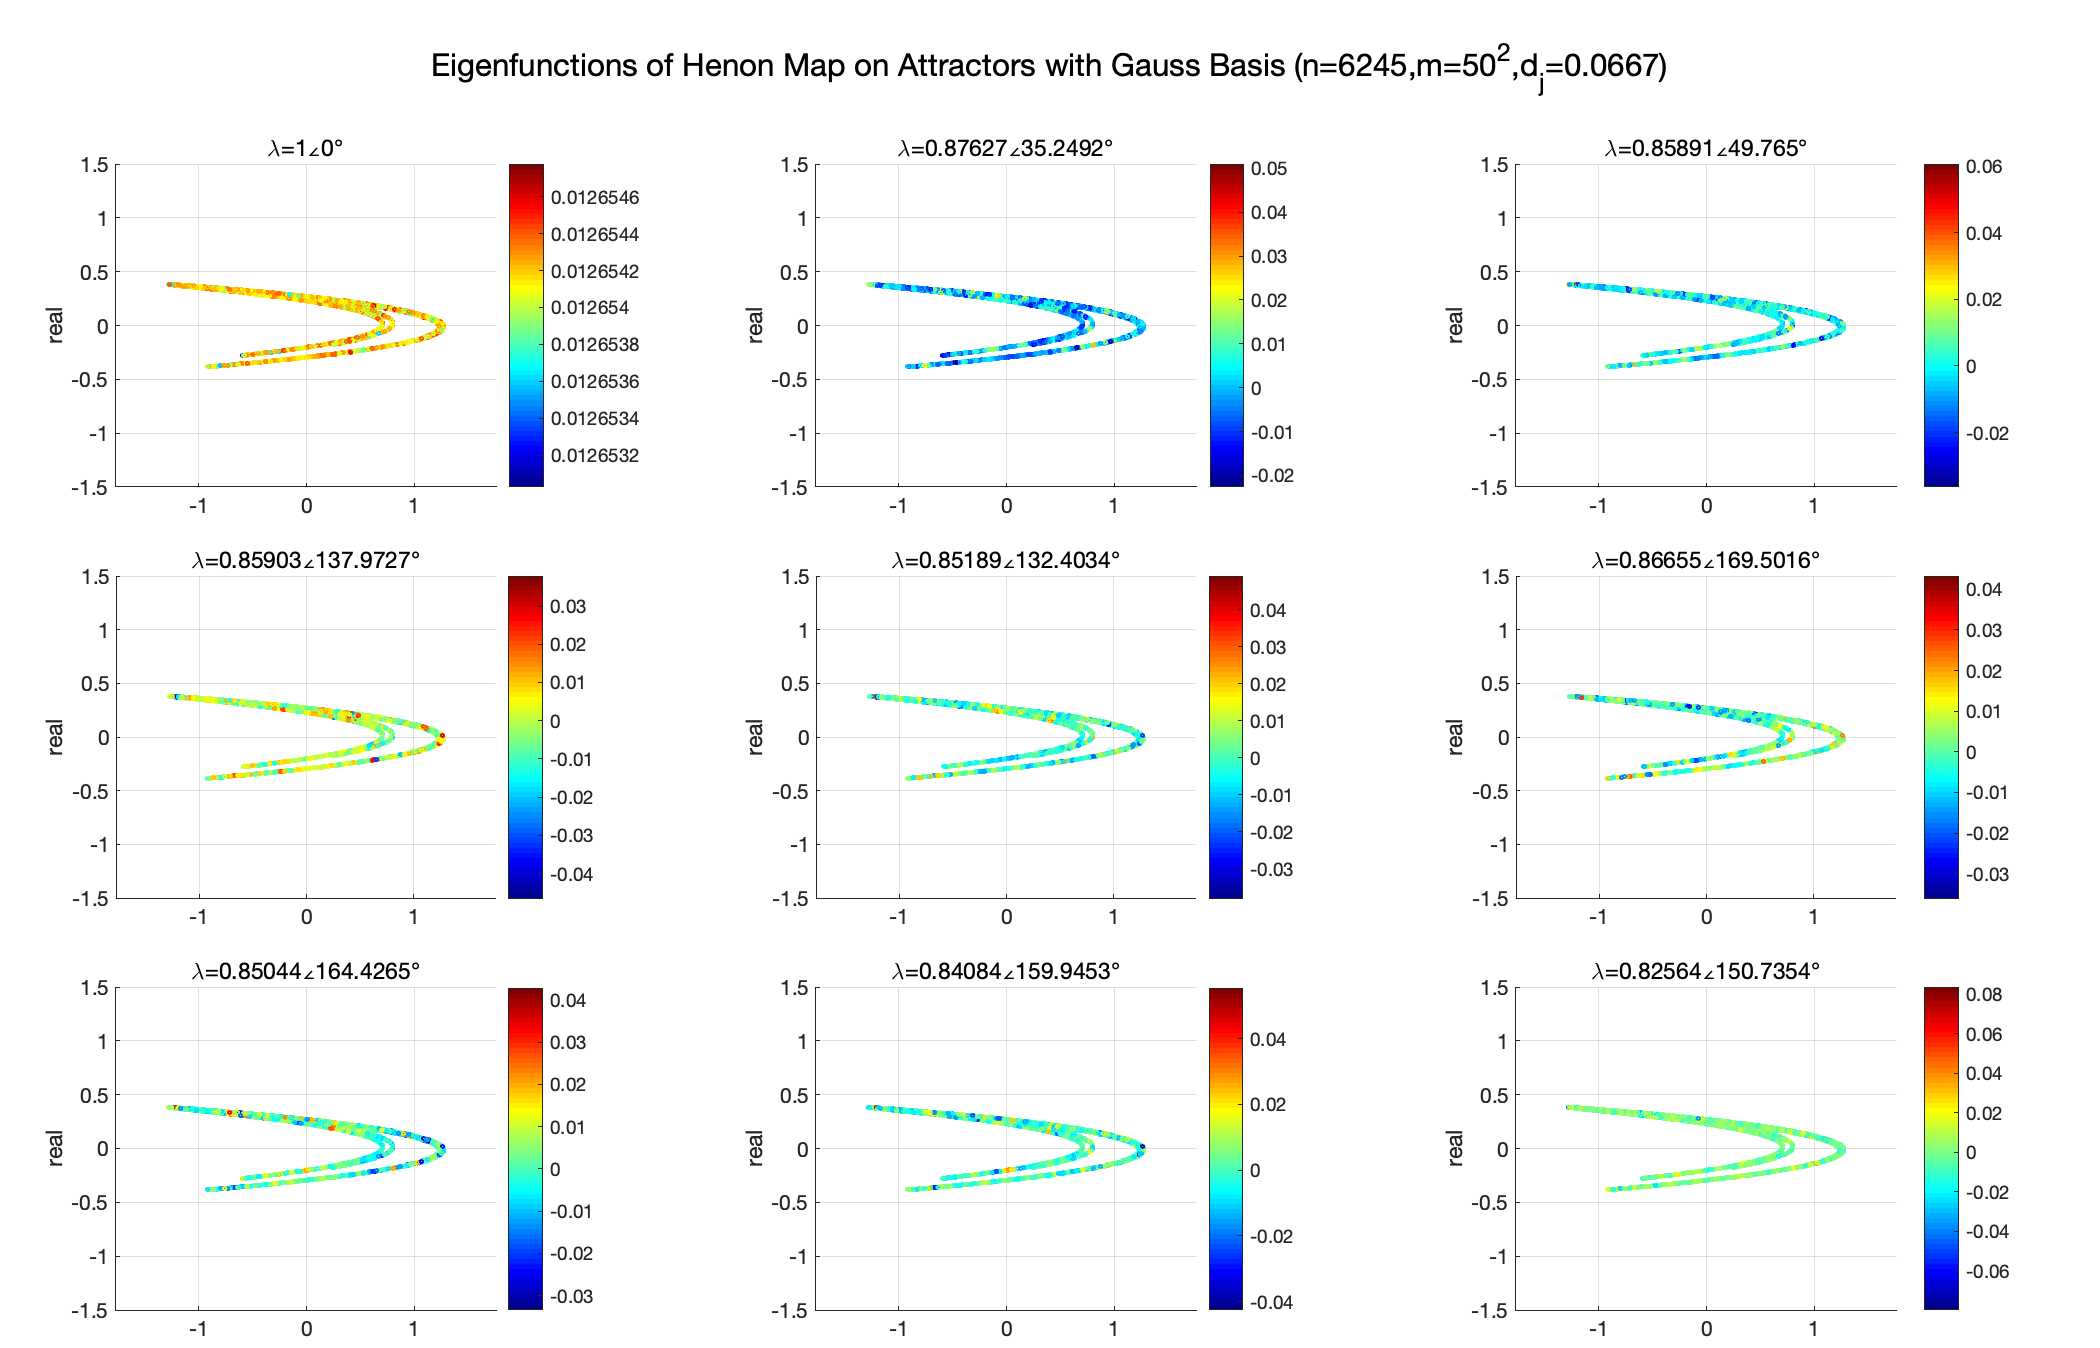
\includegraphics[scale=0.4]{henon/Henon_eigen_Gauss_attr_n6245m50md45}}
  \\
  \subfloat[鸟瞰图]{
    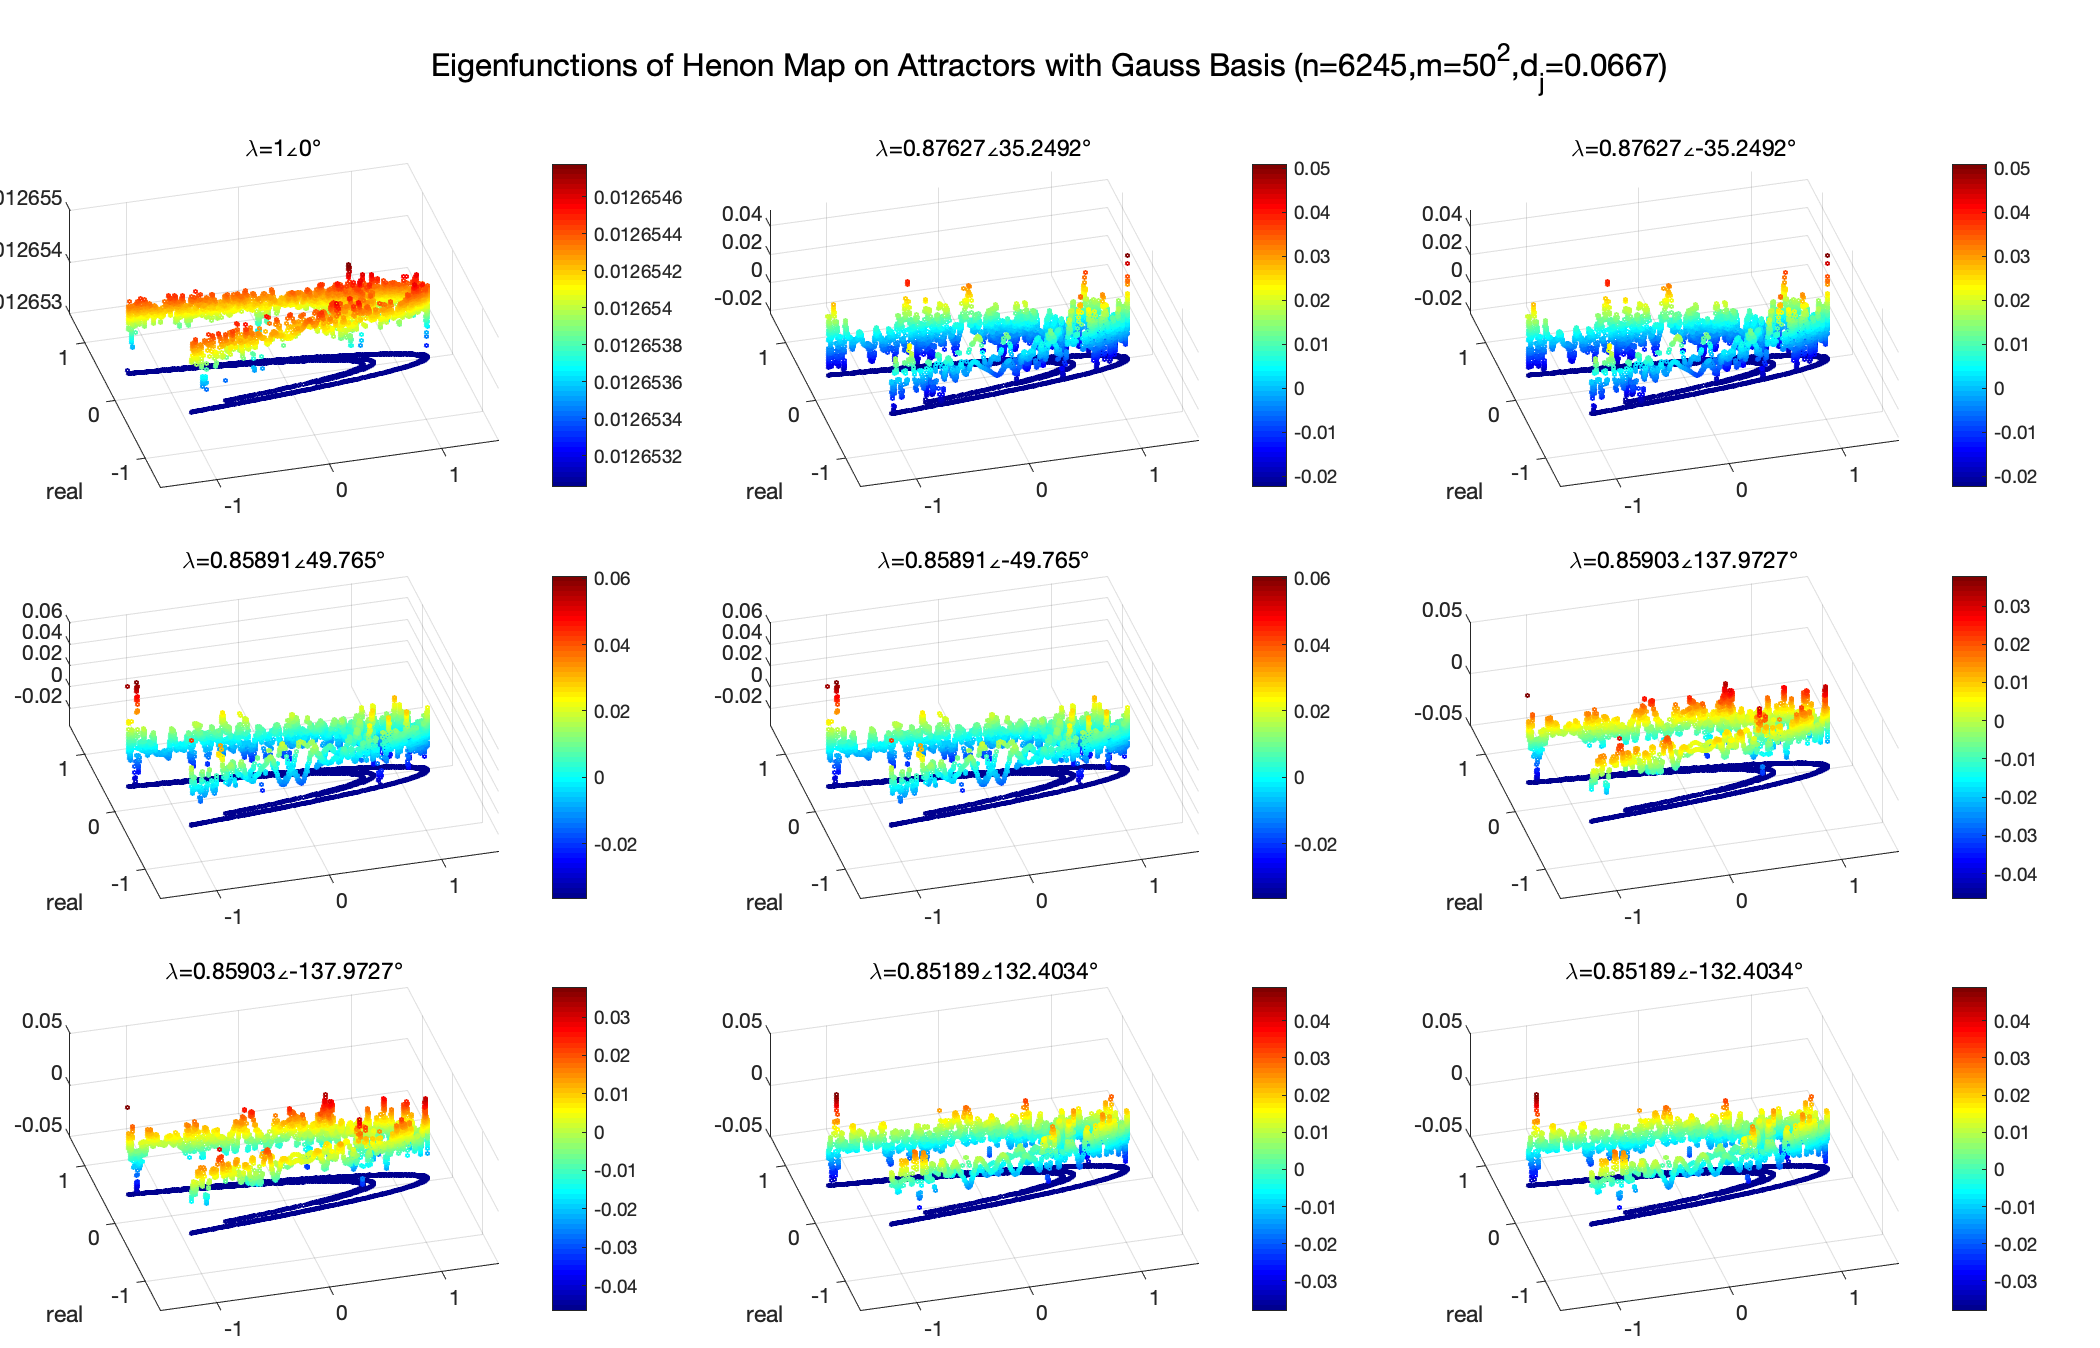
\includegraphics[scale=0.4]{henon/Henon_eigen_Gauss_attr_n6245m50}}
  \\
  \caption[埃农映射高斯基函数下在吸引子上的本征函数]{埃农映射高斯基函数下在吸引子上的本征函数($n=6245$,$m=50^2,$,$d_j=\frac{3}{45}$)}\label{fig:Henon_eigen_Gauss_attr_n6245m50md45}
\end{figure}

图\ref{fig:Henon_eigen_Gauss_attr_leftU_n6245m2}画出了当$m=2^2,3^2,4^2$时,埃农映射在吸引子域上的本征函数图像,且最多取其前9个本征函数。从图中可以看出,随着基函数数量的增加,本征函数的极值点也随之增加。
\begin{figure}
  \centering
  \subfloat[m=2]{
    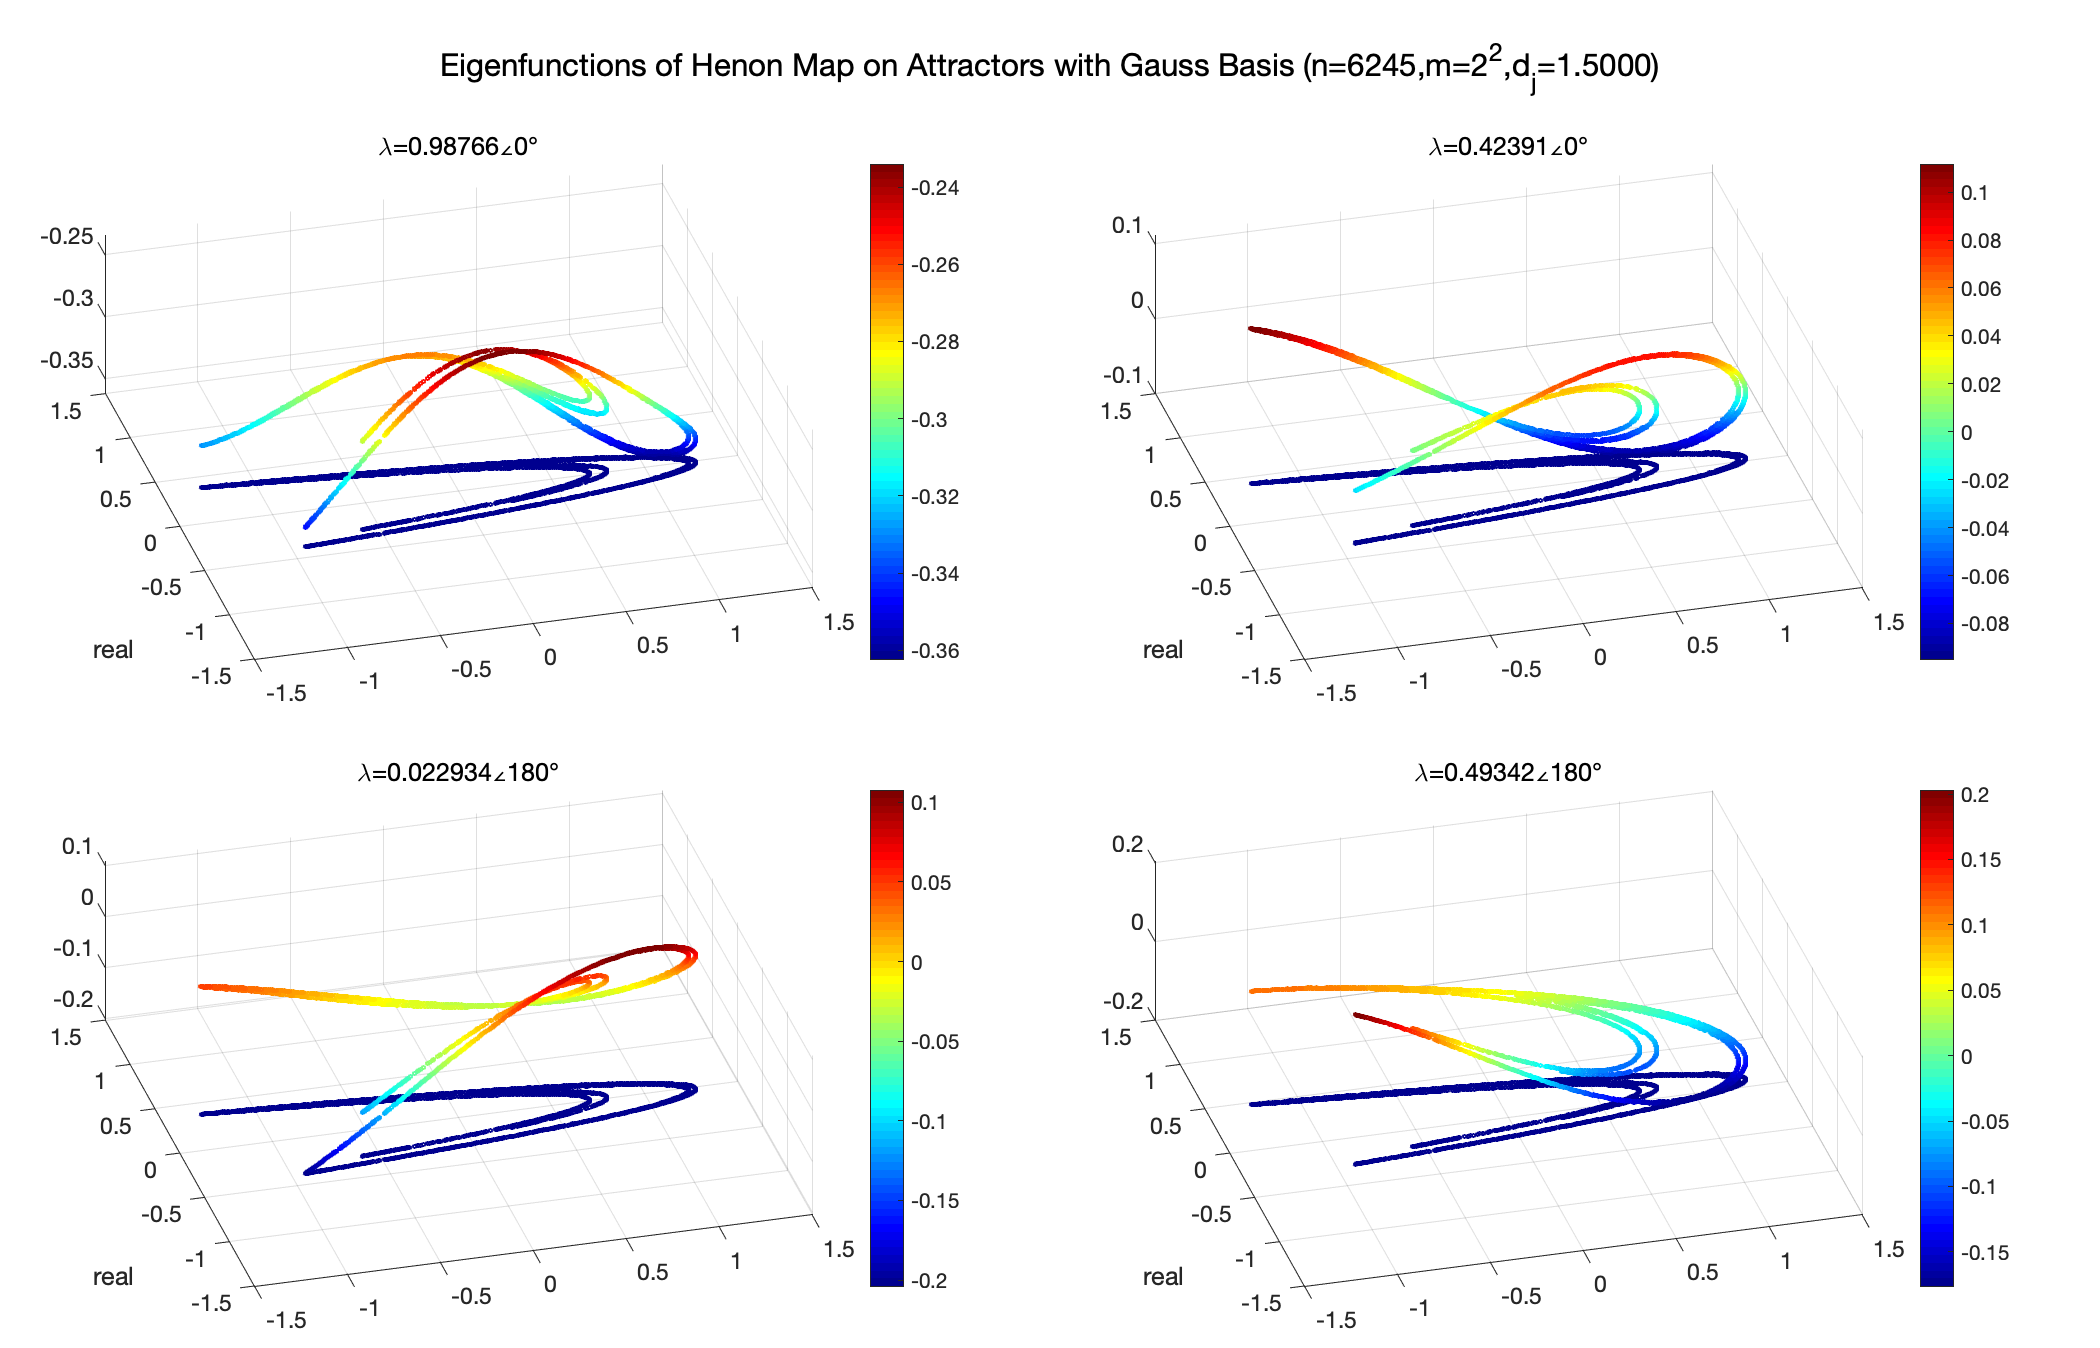
\includegraphics[scale=0.28]{henon/Henon_eigen_Gauss_attr_leftU_n6245m2}}
  \\
  \subfloat[m=3]{
    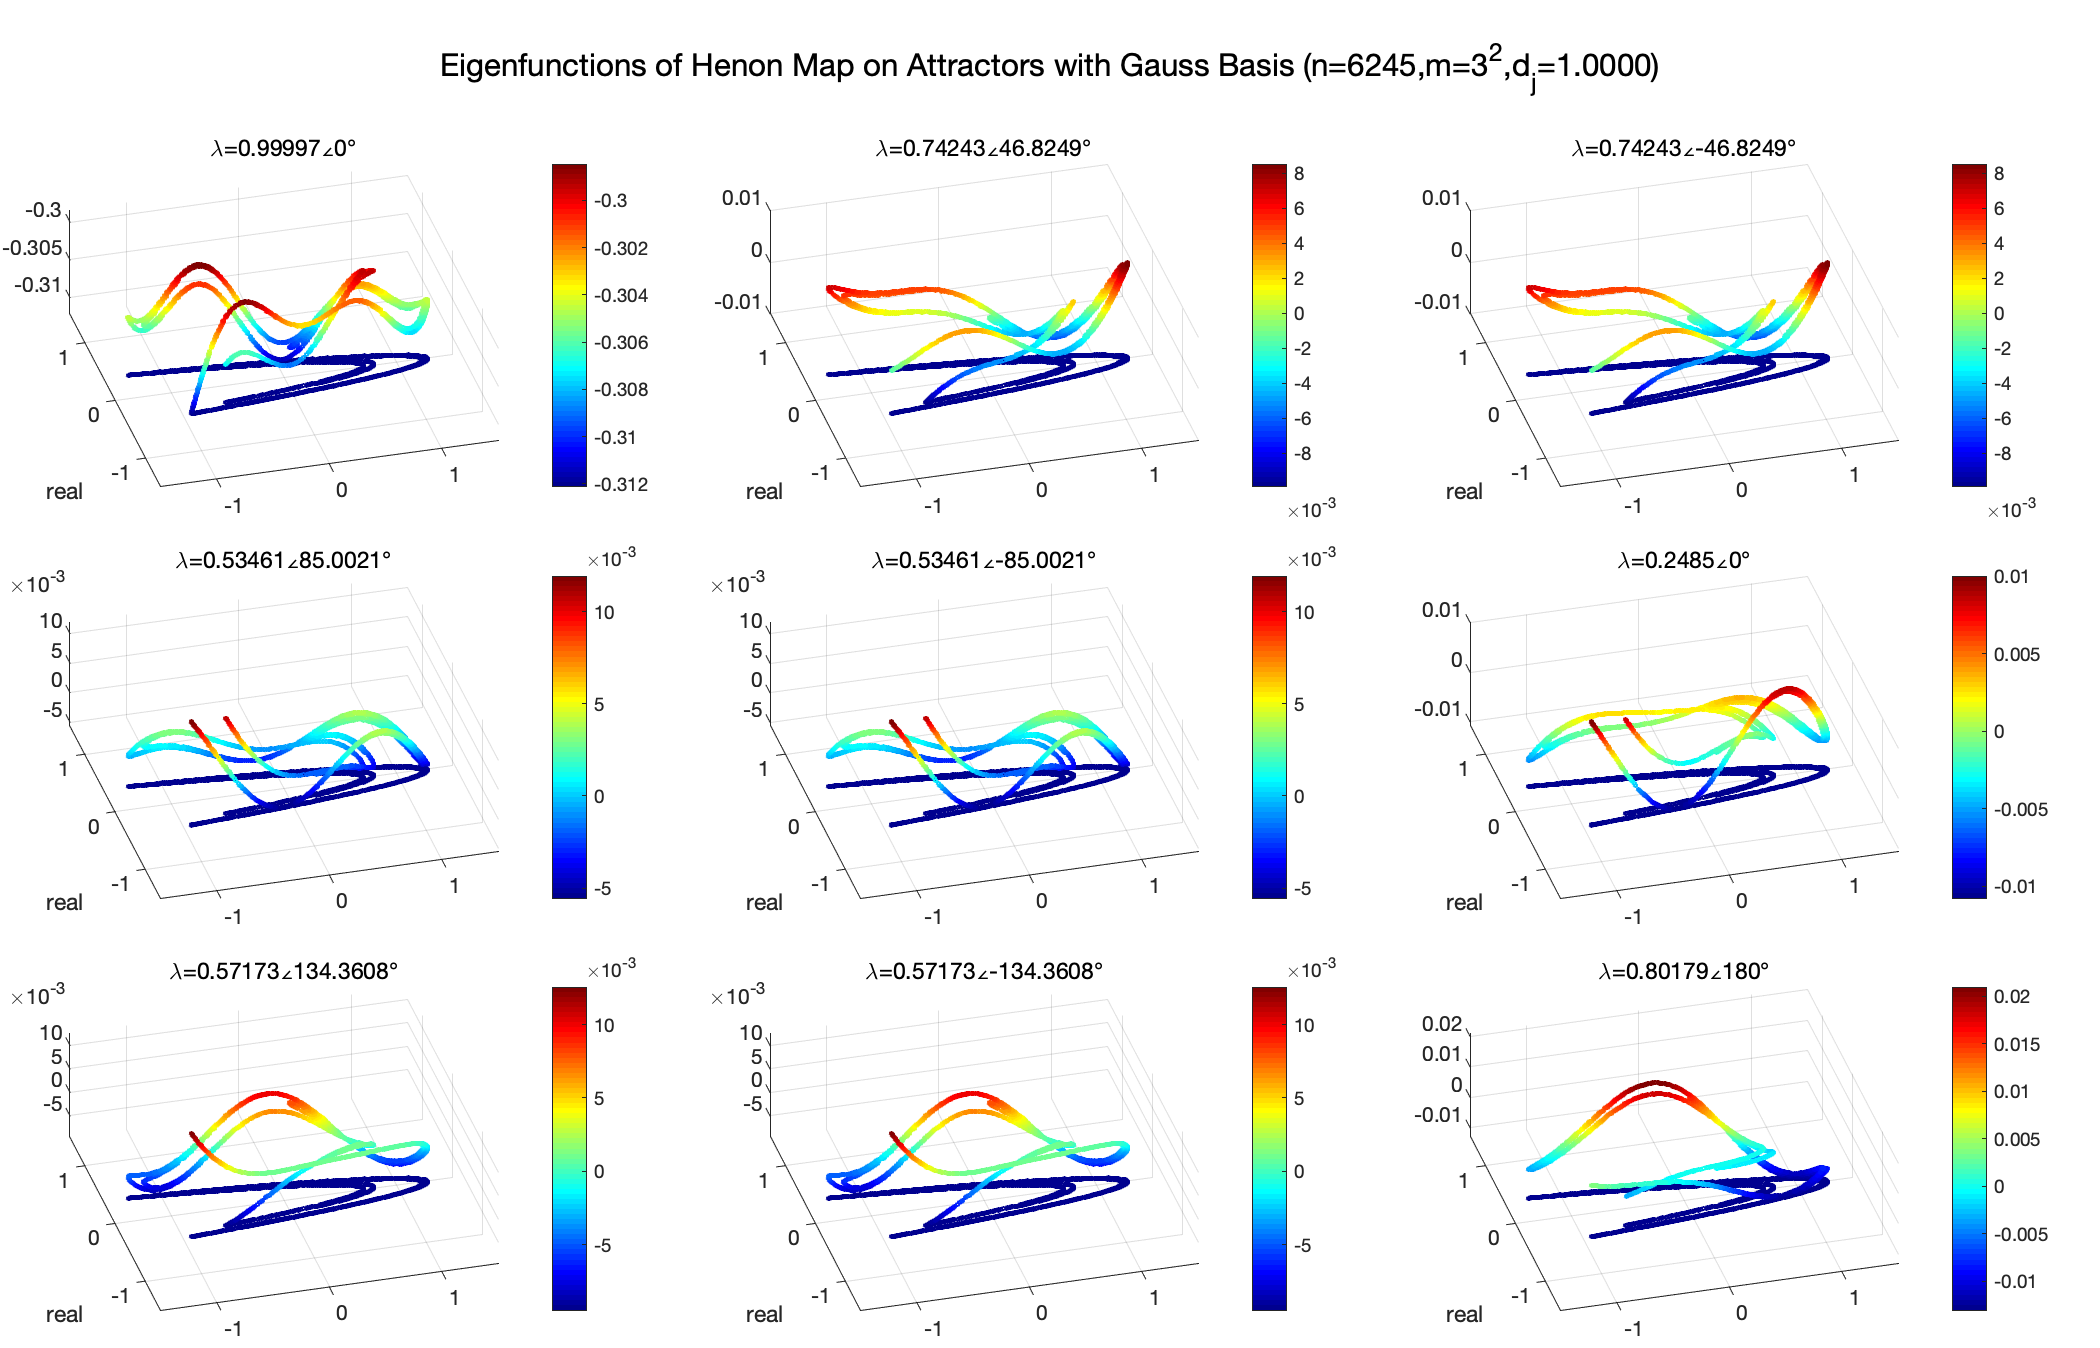
\includegraphics[scale=0.28]{henon/Henon_eigen_Gauss_attr_leftU_n6245m3}}
  \\
  \subfloat[m=4]{
    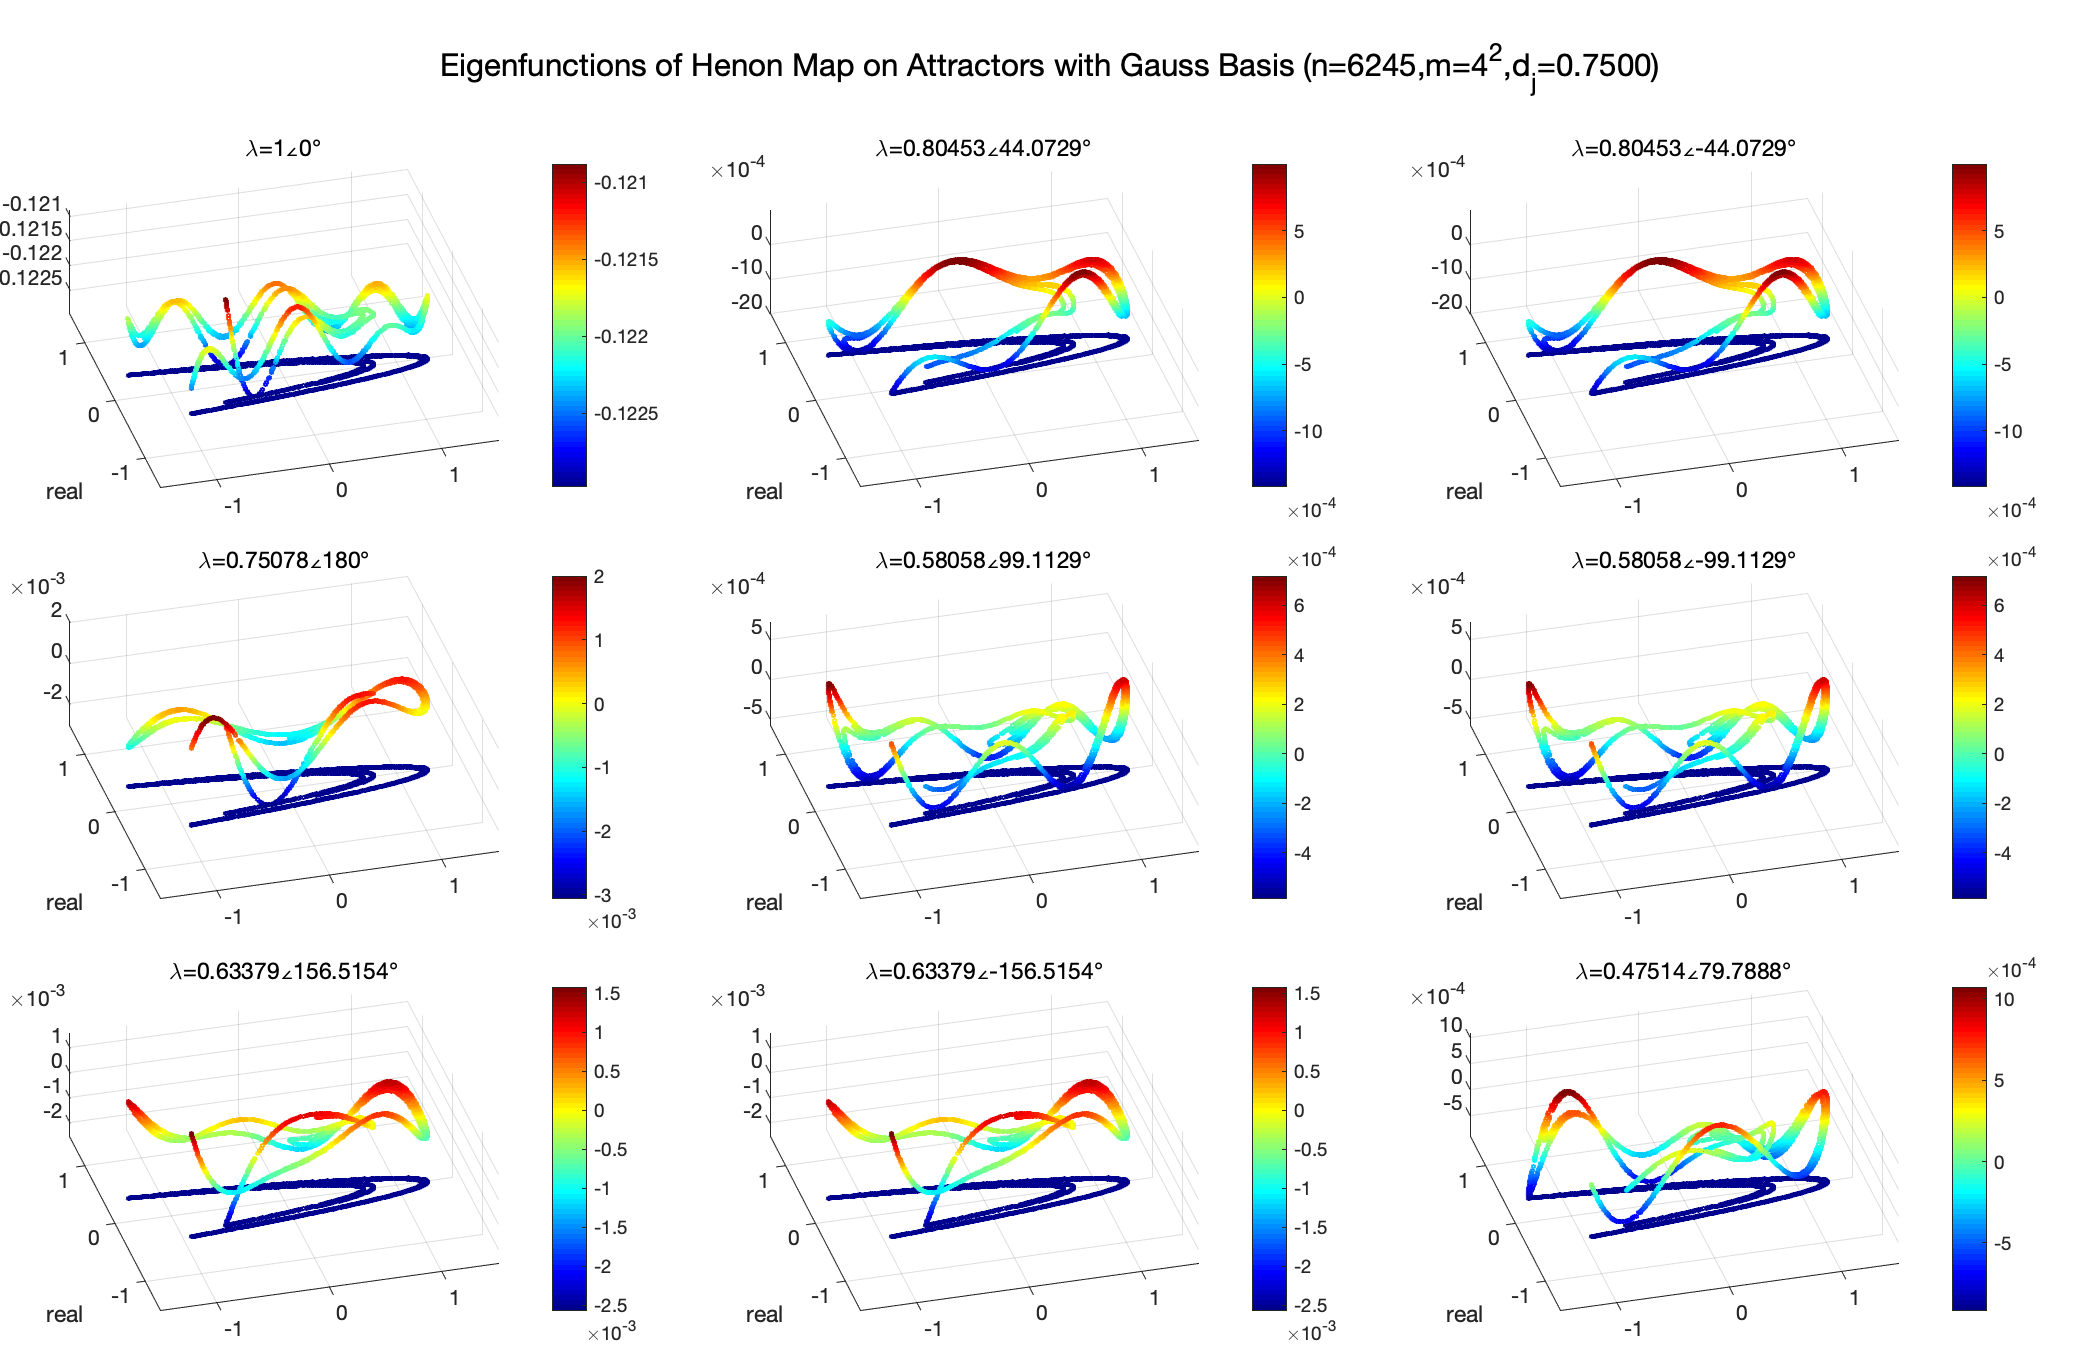
\includegraphics[scale=0.28]{henon/Henon_eigen_Gauss_attr_leftU_n6245m4}}
  \\
  \caption{埃农映射高斯基函数下在吸引子上的本征函数($n=6245$)}\label{fig:Henon_eigen_Gauss_attr_leftU_n6245m2}
\end{figure}

\subsubsection{自然基函数空间}
在式\eqref{eq:Koop_kl2}中,我们可以通过构造自然函数格点来计算Koopman算符的本征值与本征函数,但这与在一维的情况稍有不同,自然基函数是由粒子的演化得到的,而二维映射中存在两组演化,且每组演化都可以作为一组自然基函数,所以我们在求本征函数时需要区分演化的维度,即是x方向的本征函数还是y方向的本征函数。同时,由于自然演化在埃农映射中并不能遍布整个相空间:因为埃农映射并不是相空间到自身的映射,且其存在收缩性,故我们不能将本征函数画在整个相空间中。但是在埃农映射中存在一吸引子区域满足到自身的映射,在吸引子上的粒子可以通过迭代映射遍历整个吸引子,于是在自然基函数空间中,我们选取吸引子作为我们的相空间,在吸引子区域作出本征函数图像。

图\ref{fig:Henon_eigen_natural_n2000m4_figure1}画出了在演化格点数量$n=2000$,自然基函数数量$m=4$时,不同本征值下的埃农映射在吸引子域上的本征函数图像,由于吸引子域较小不易表示,我们在每个子图中分为四个小图,其中前两个小图表示x方向和y方向上的本征函数的三维鸟瞰图及其在xy平面上的投影,后两个小图表示二维中的本征函数图像。
\begin{figure}
    \centering
    \subfloat{
      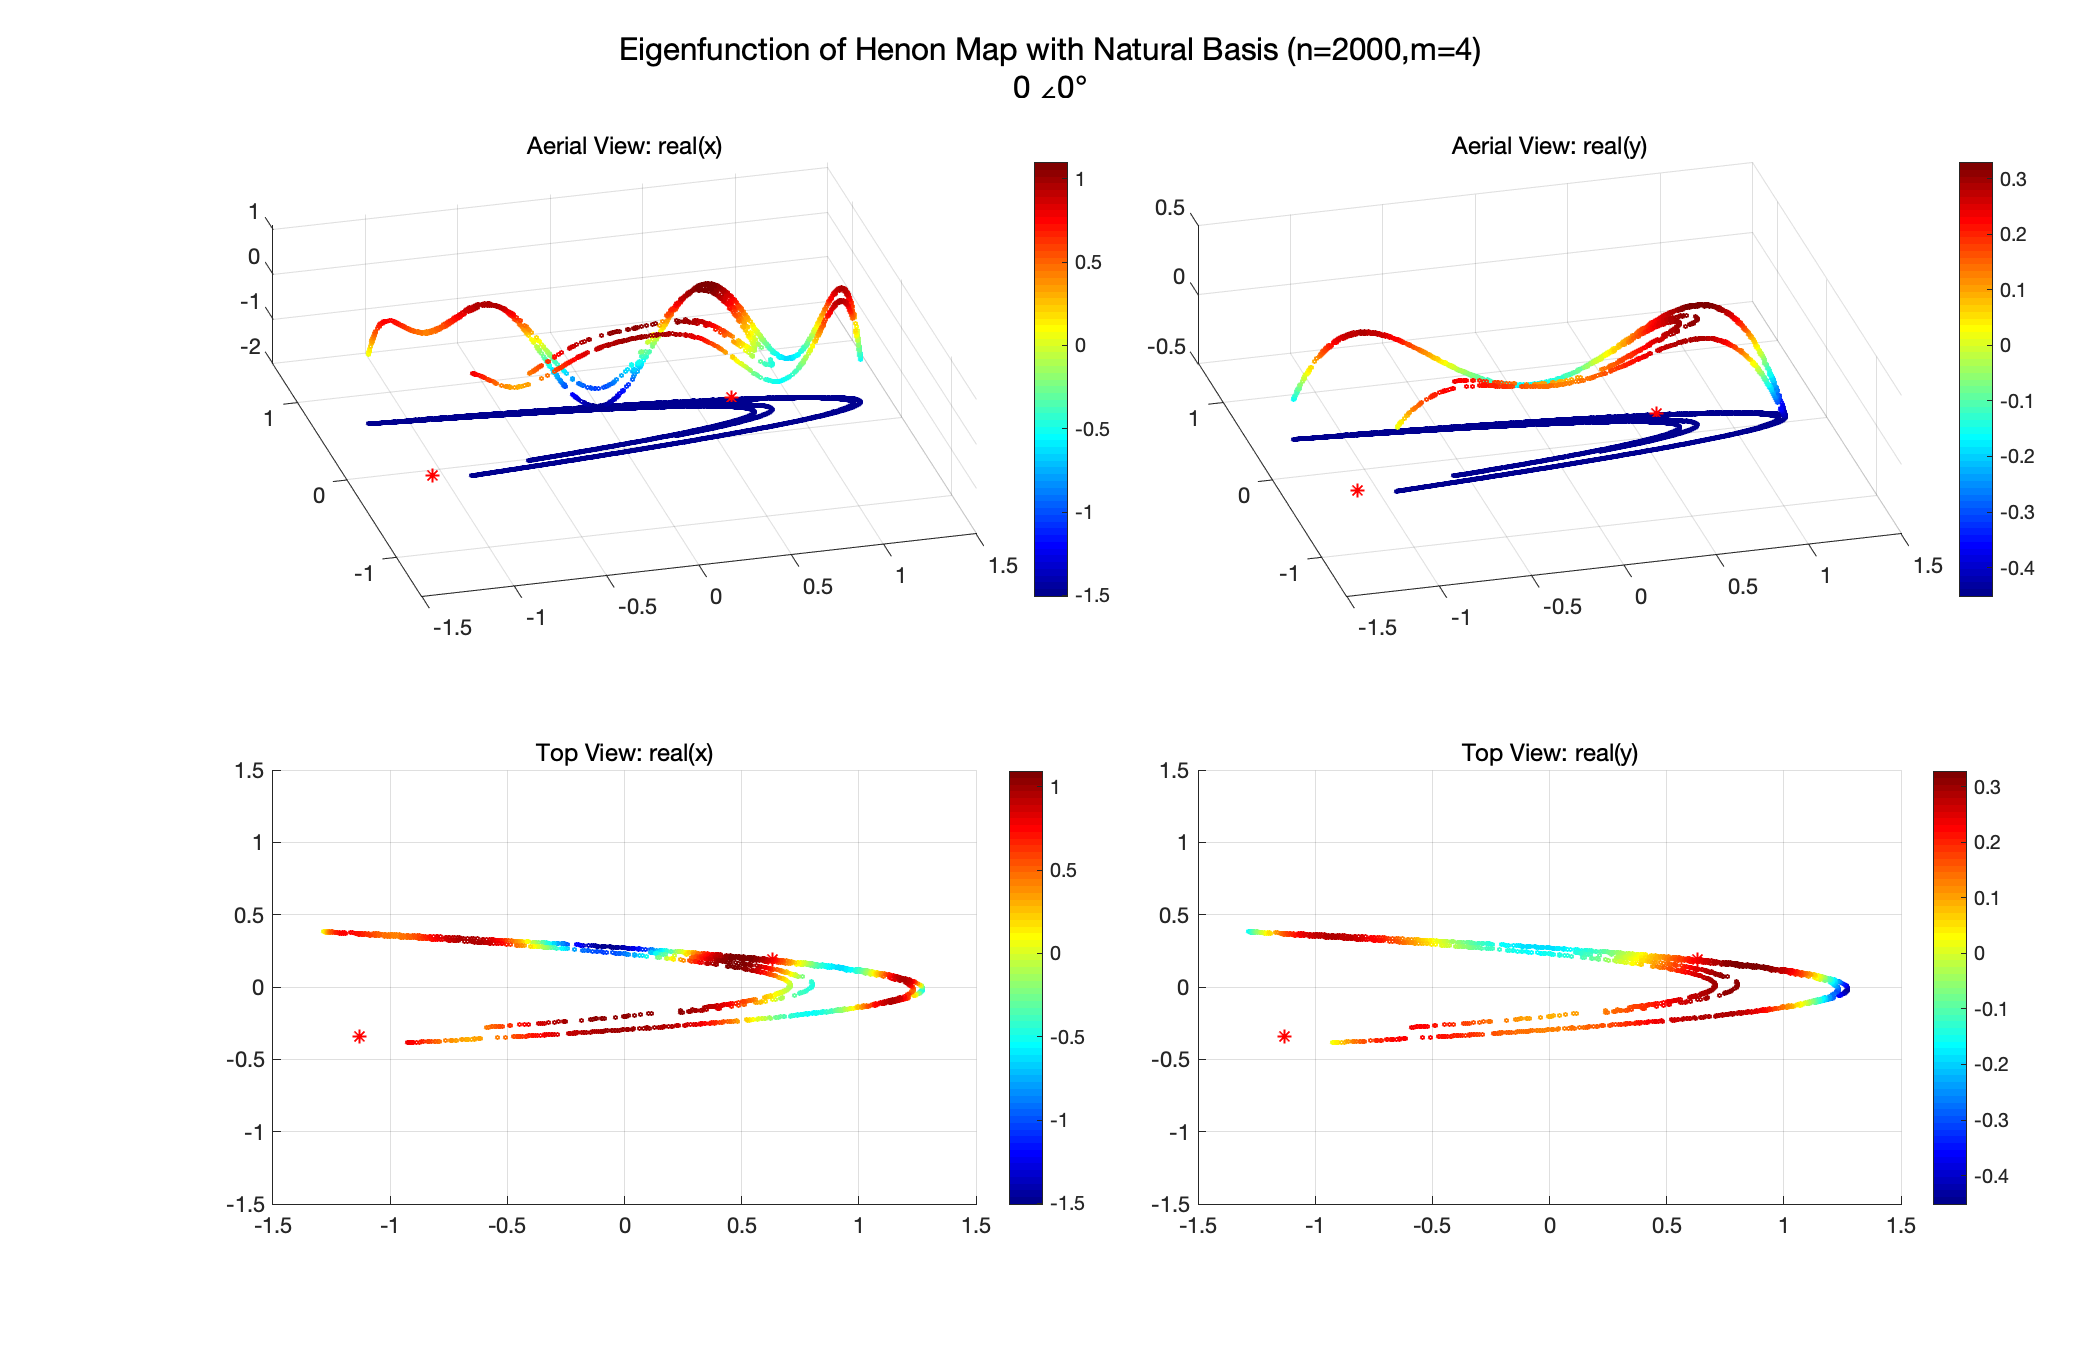
\includegraphics[scale=0.2]{henon/natural/Henon_eigen_natural_n2000m4_figure1}}
    \subfloat{
      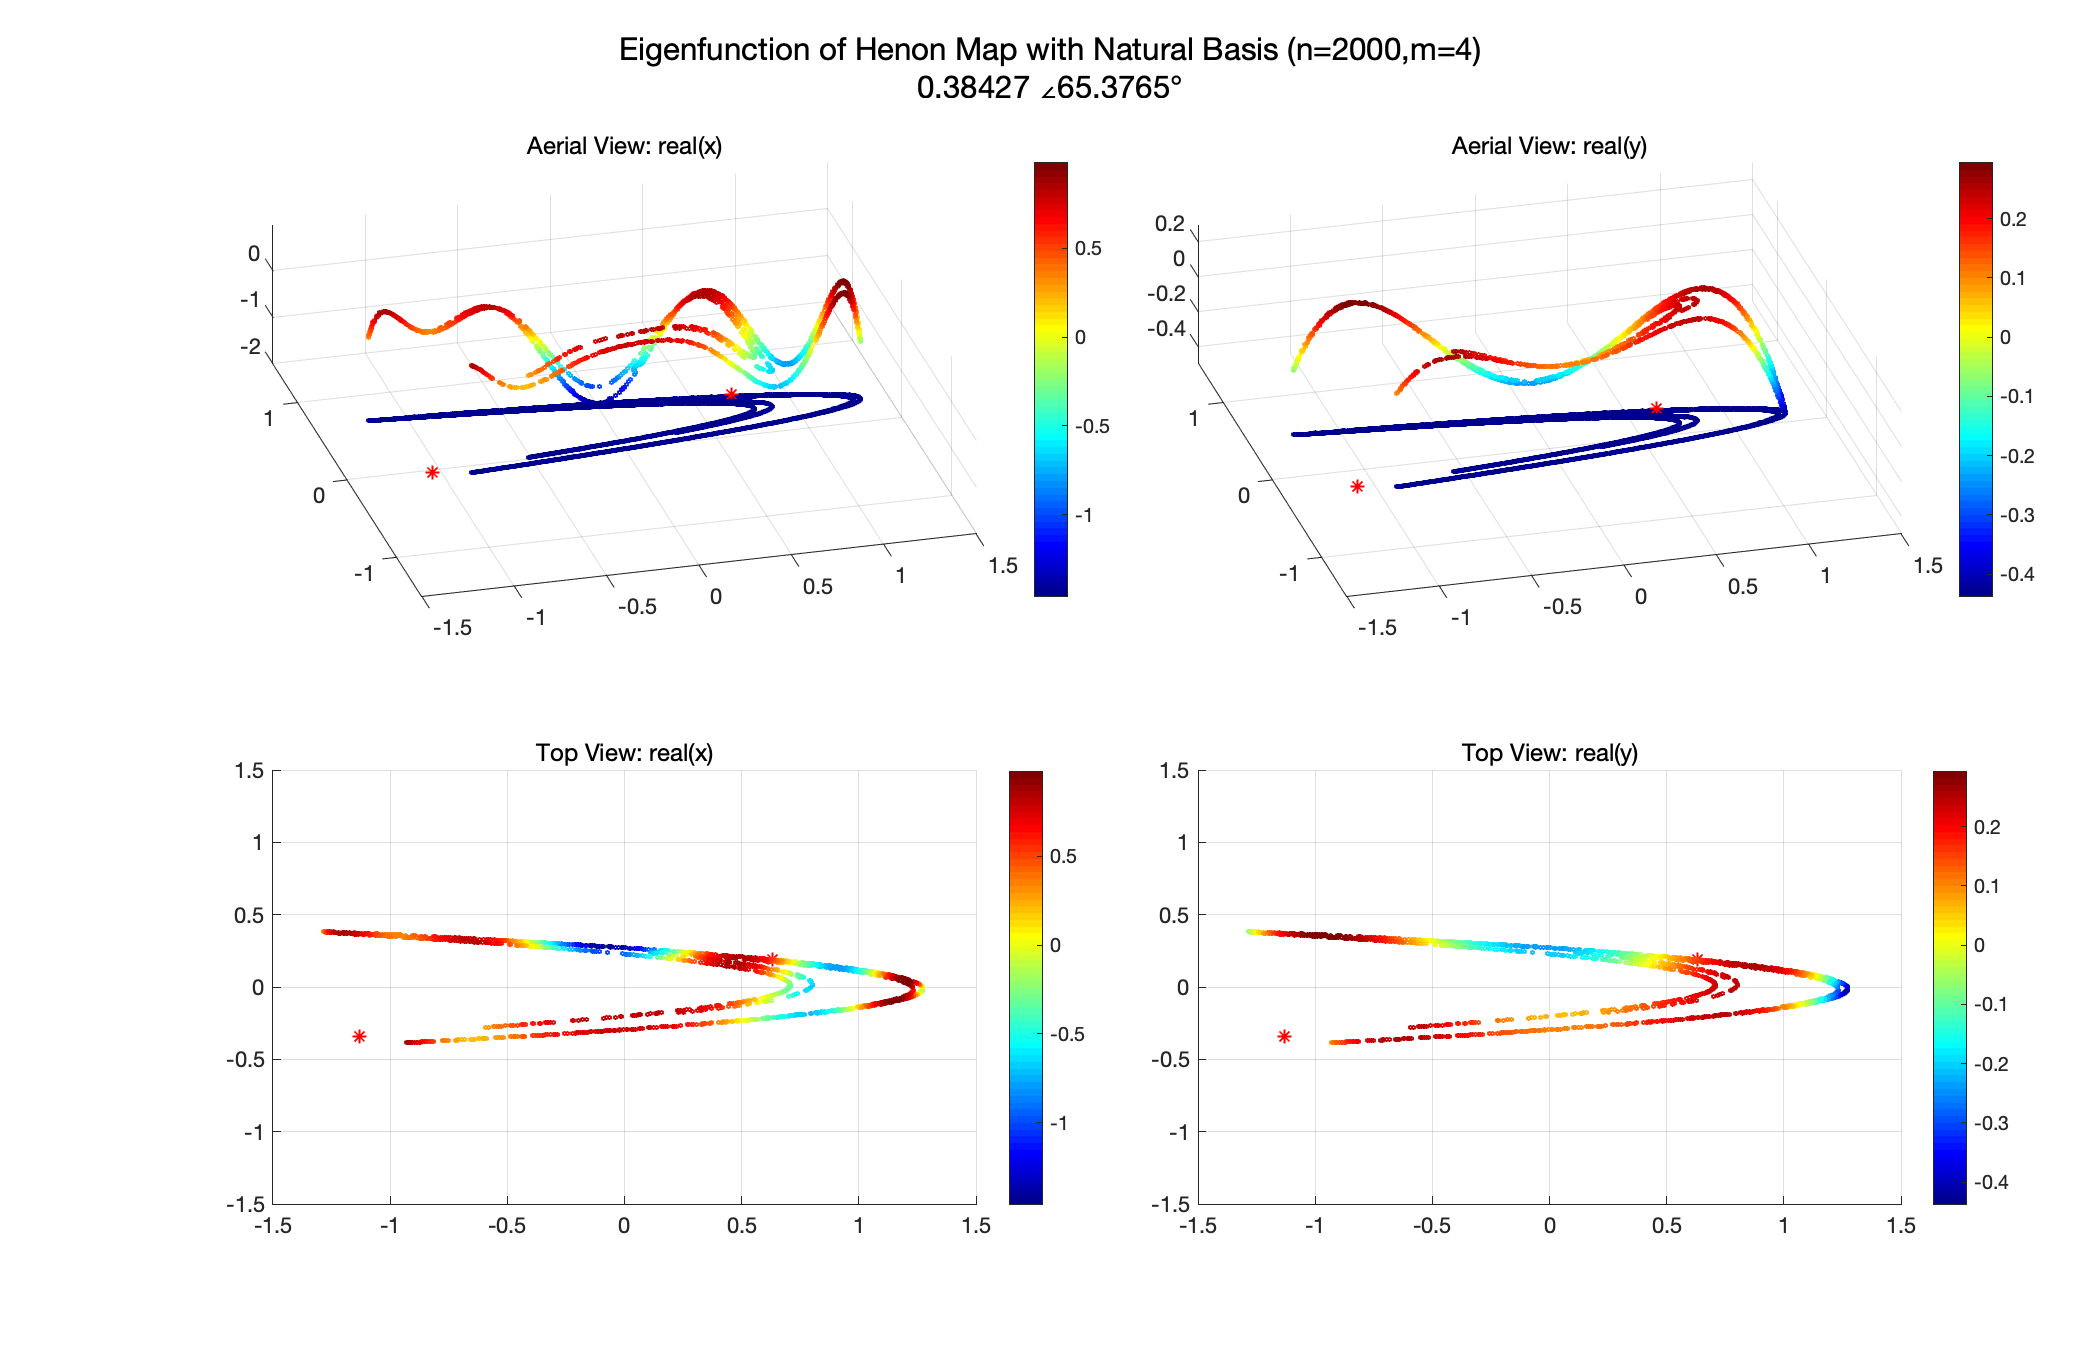
\includegraphics[scale=0.2]{henon/natural/Henon_eigen_natural_n2000m4_figure2}}
    \\
    \subfloat{
      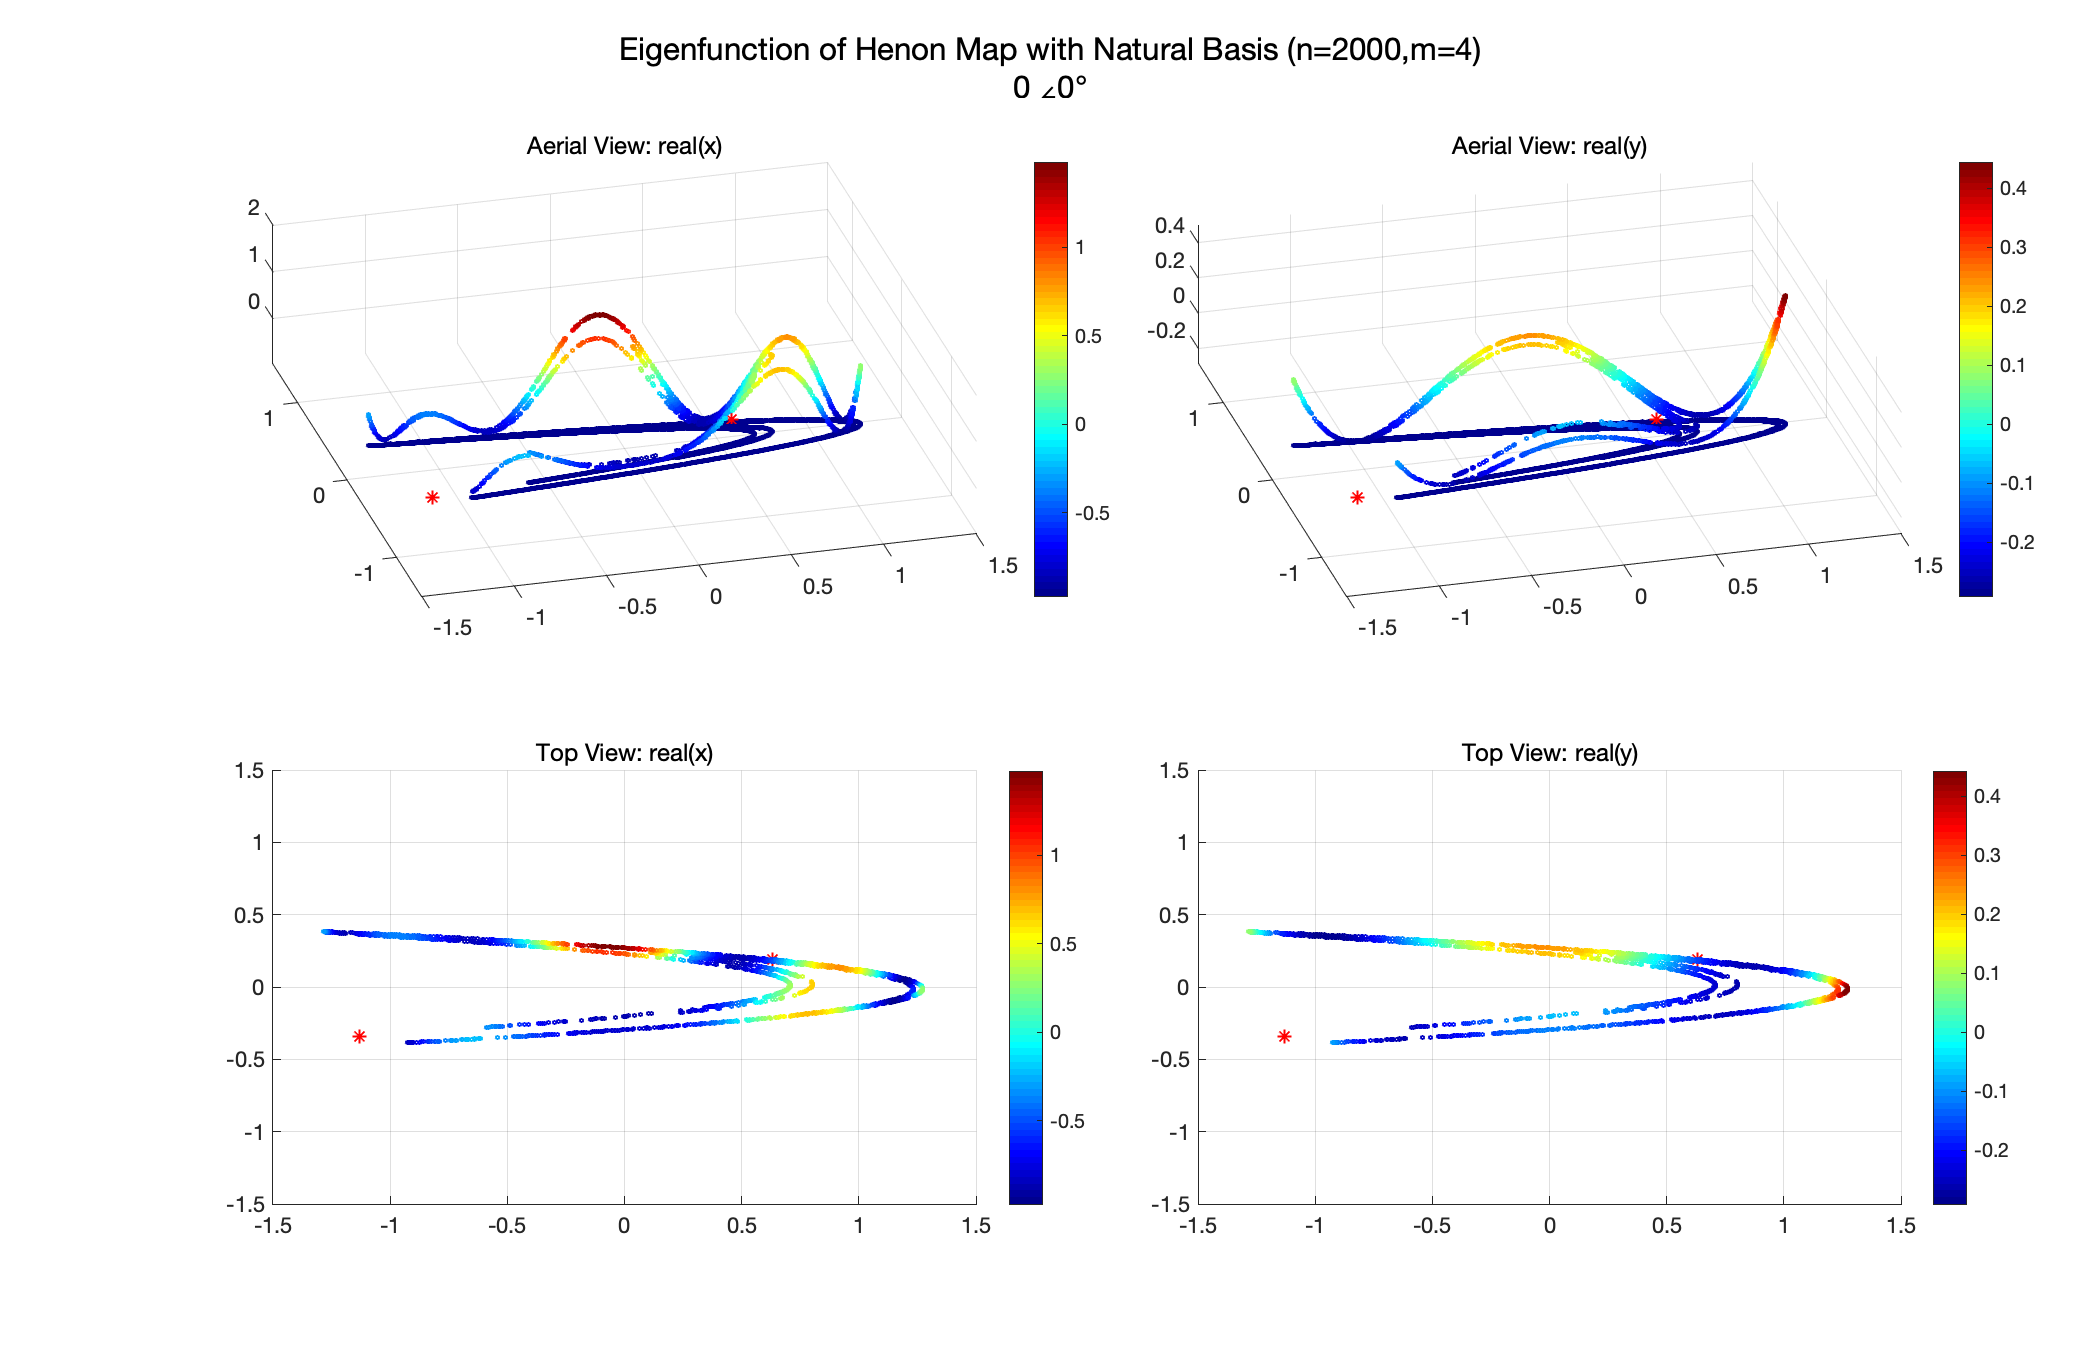
\includegraphics[scale=0.2]{henon/natural/Henon_eigen_natural_n2000m4_figure3}}
    \subfloat{
      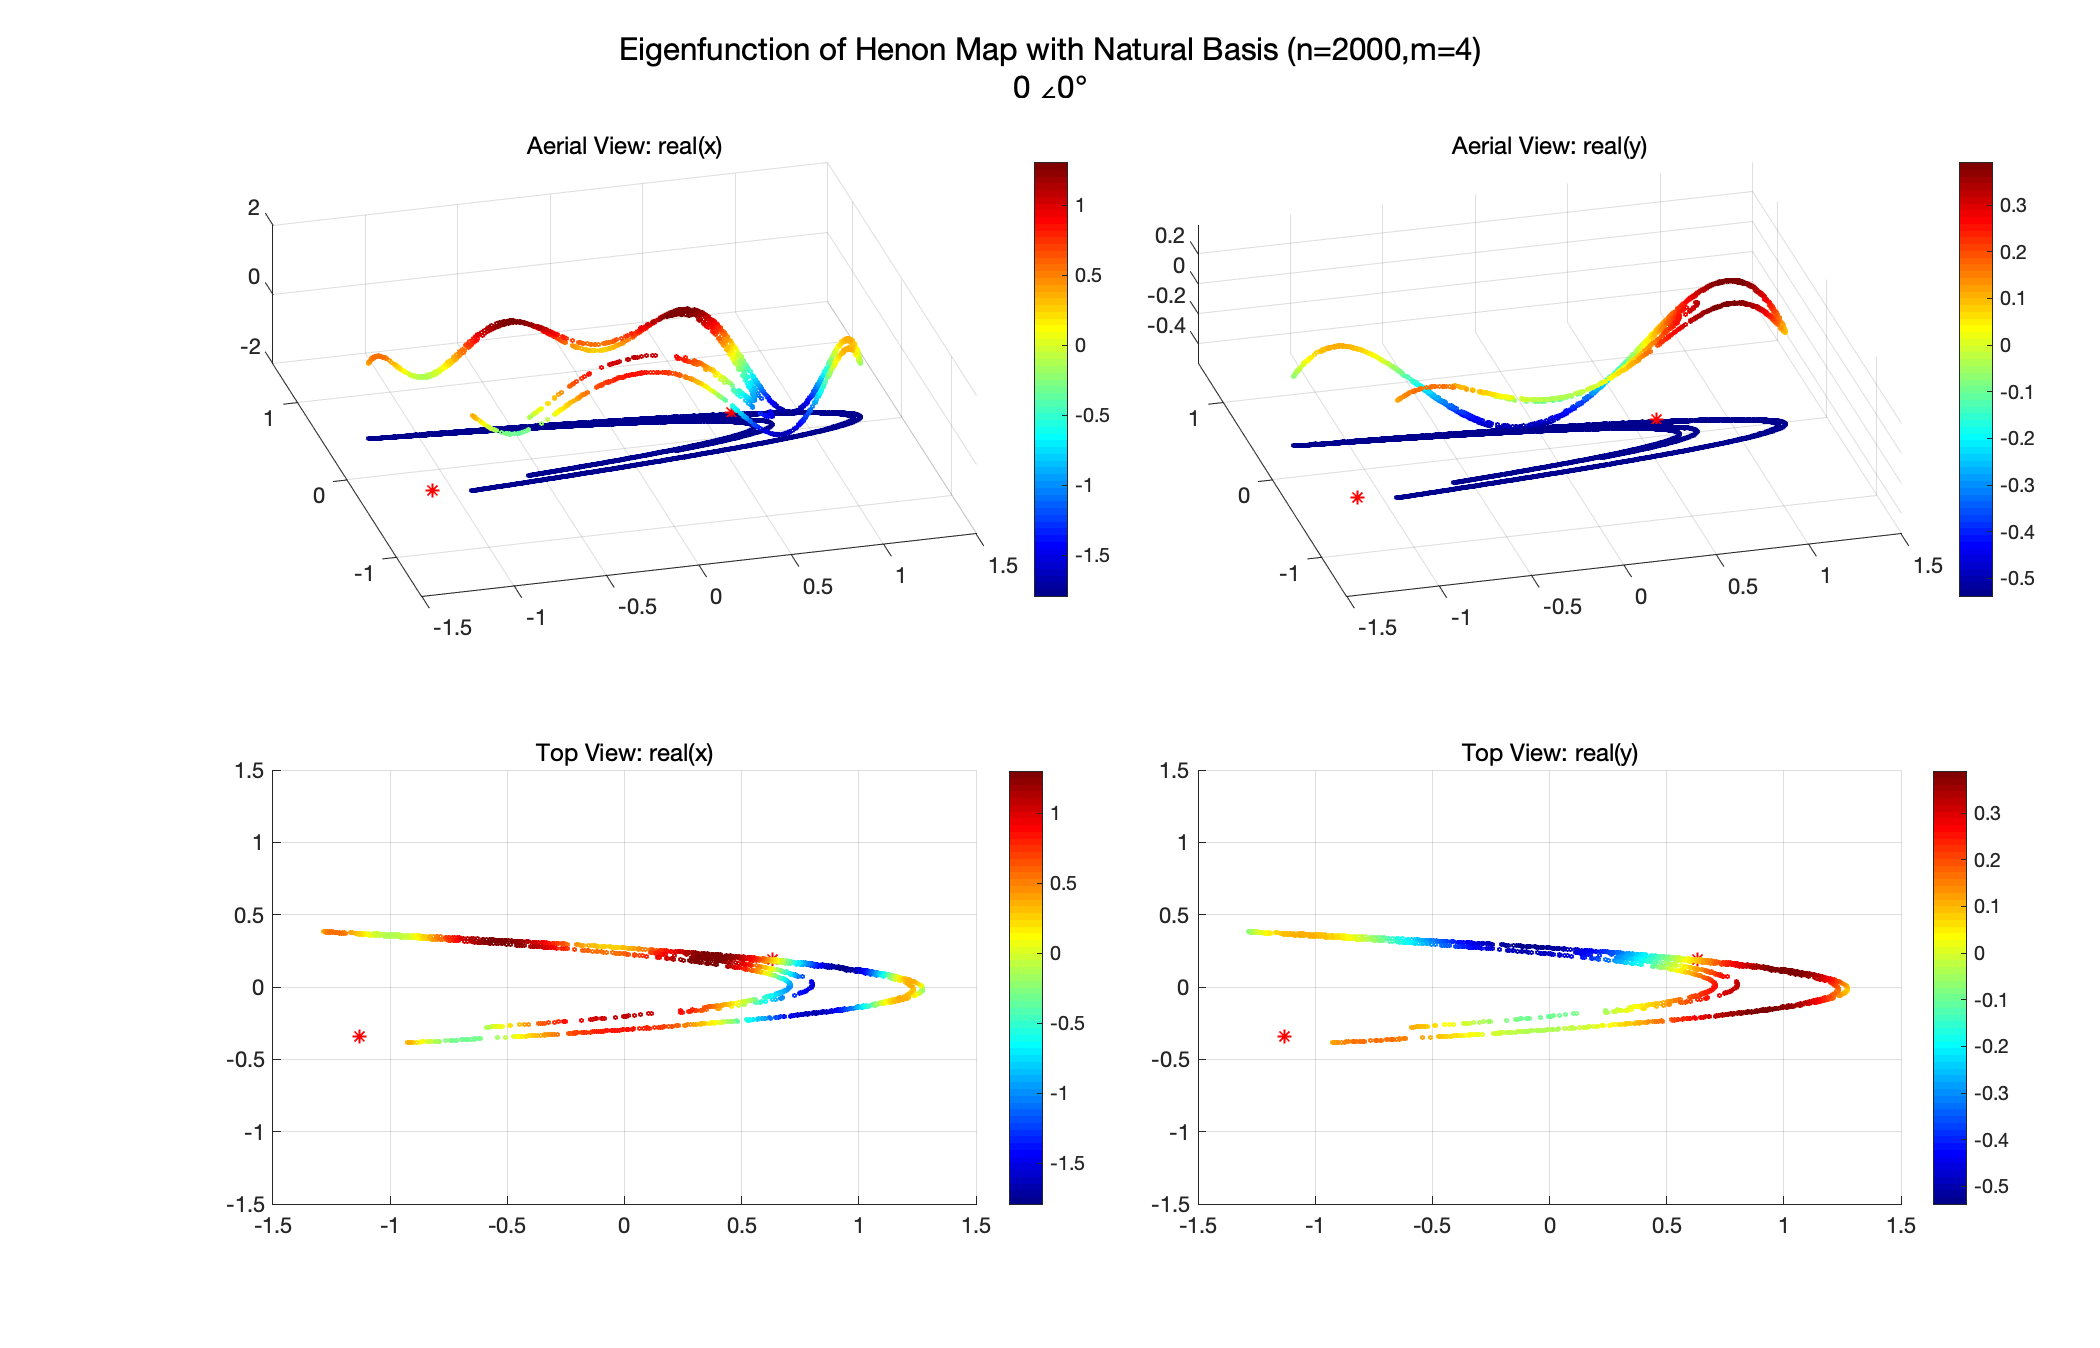
\includegraphics[scale=0.2]{henon/natural/Henon_eigen_natural_n2000m4_figure4}}
    \\
    \caption[埃农映射自然基函数下的本征函数]{埃农映射自然基函数下的本征函数($n=2000$,$m=4$):每个子图表示不同本征值下的本征函数图像,其中每个子图又分为四个小图,其中前两个小图表示两个方向上的本征函数的三维鸟瞰图及其在二维的投影,后两个小图表示二维中的本征函数}\label{fig:Henon_eigen_natural_n2000m4_figure1}
\end{figure}

我们可以在图\ref{fig:Henon_eigen_natural_n2000m4_figure1}得到与一维映射类似的一些关键点:在埃农映射的吸引子中,点$(1.25,0)$附近存在一个较明显的转折点,在这个点上的本征函数总是会出现极值点。类比一维映射中的边界点,我们可以猜测这个点也可能具有与一维映射相似的性质。

图\ref{fig:Henon_eigen_natural_n2000m1}画出了当基函数数量$m=1,2,3,4,5,6,7,8,9$时关于x方向上的所有m个本征函数图像。随着基函数数量的增加,本征函数图像的结构也变得更复杂,且基函数数量每增加1,极值点出现的数量增加近似一倍,这与我们在一维映射中的结论一致。在$m=1$时,本征函数图像有且仅由一个点,且该点将埃农映射的吸引子分为了两部分;当$m=2$时,极值点出现了三个,且多出来的两个点又将每部分分为了各自的两部分,而在埃农映射中,埃农映射$T$一次映射即体现一次弯折,多次映射$T^n$就会体现多次弯折。若我们能证明这些极值点与埃农映射的边界点一致,我们便可以得到与一维映射一致的结论。


\begin{figure}
    \centering
    \subfloat[m=1]{
      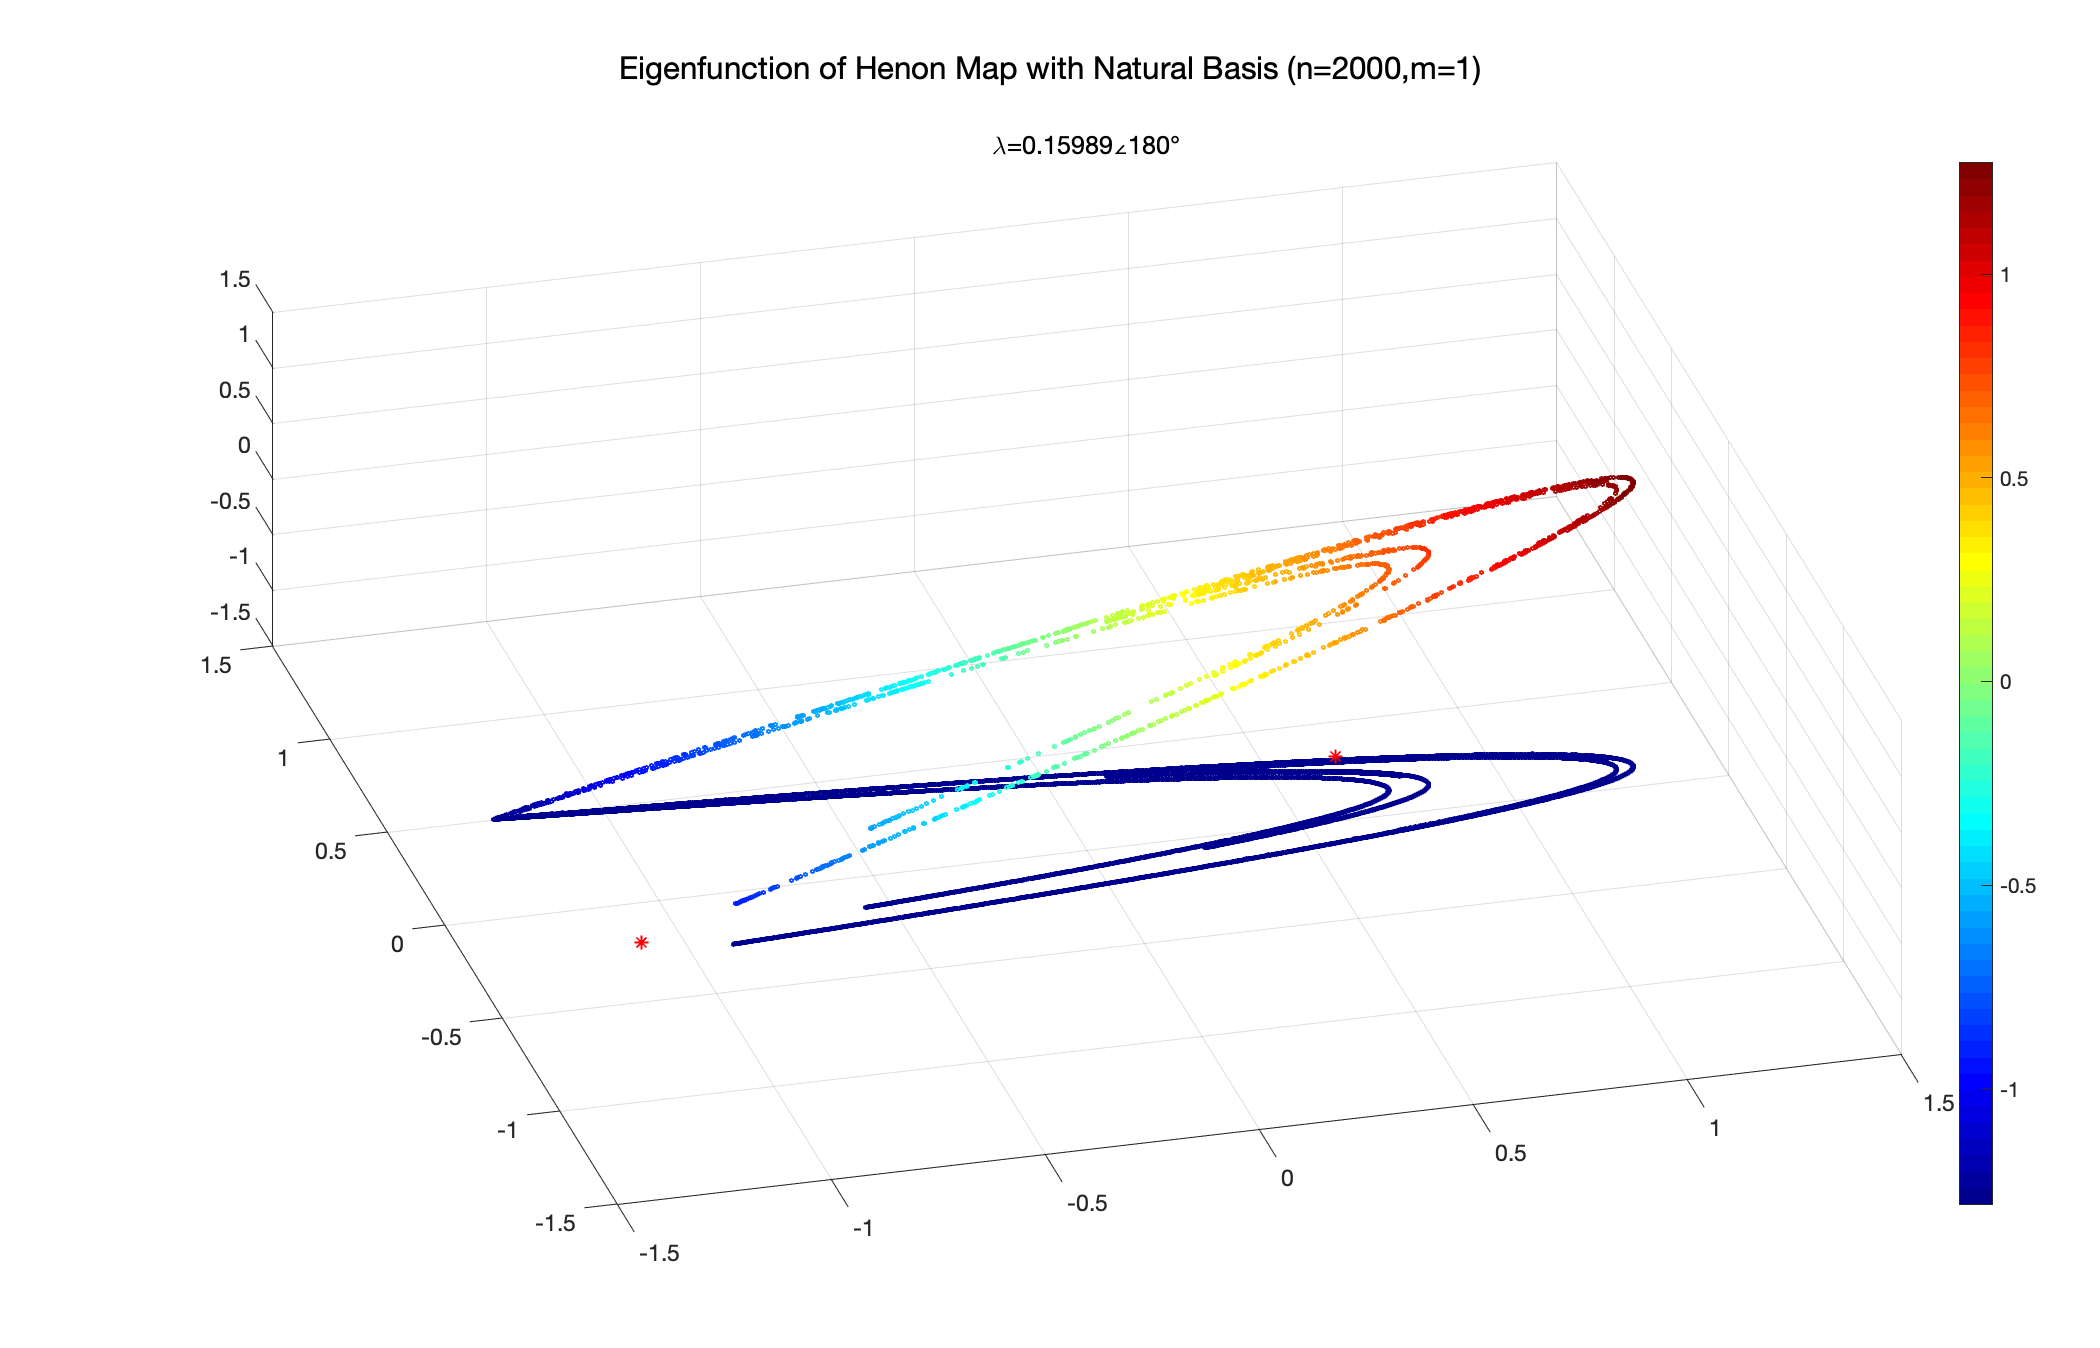
\includegraphics[scale=0.2]{henon/natural/Henon_eigen_natural_n2000m1}}
    \subfloat[m=2]{
      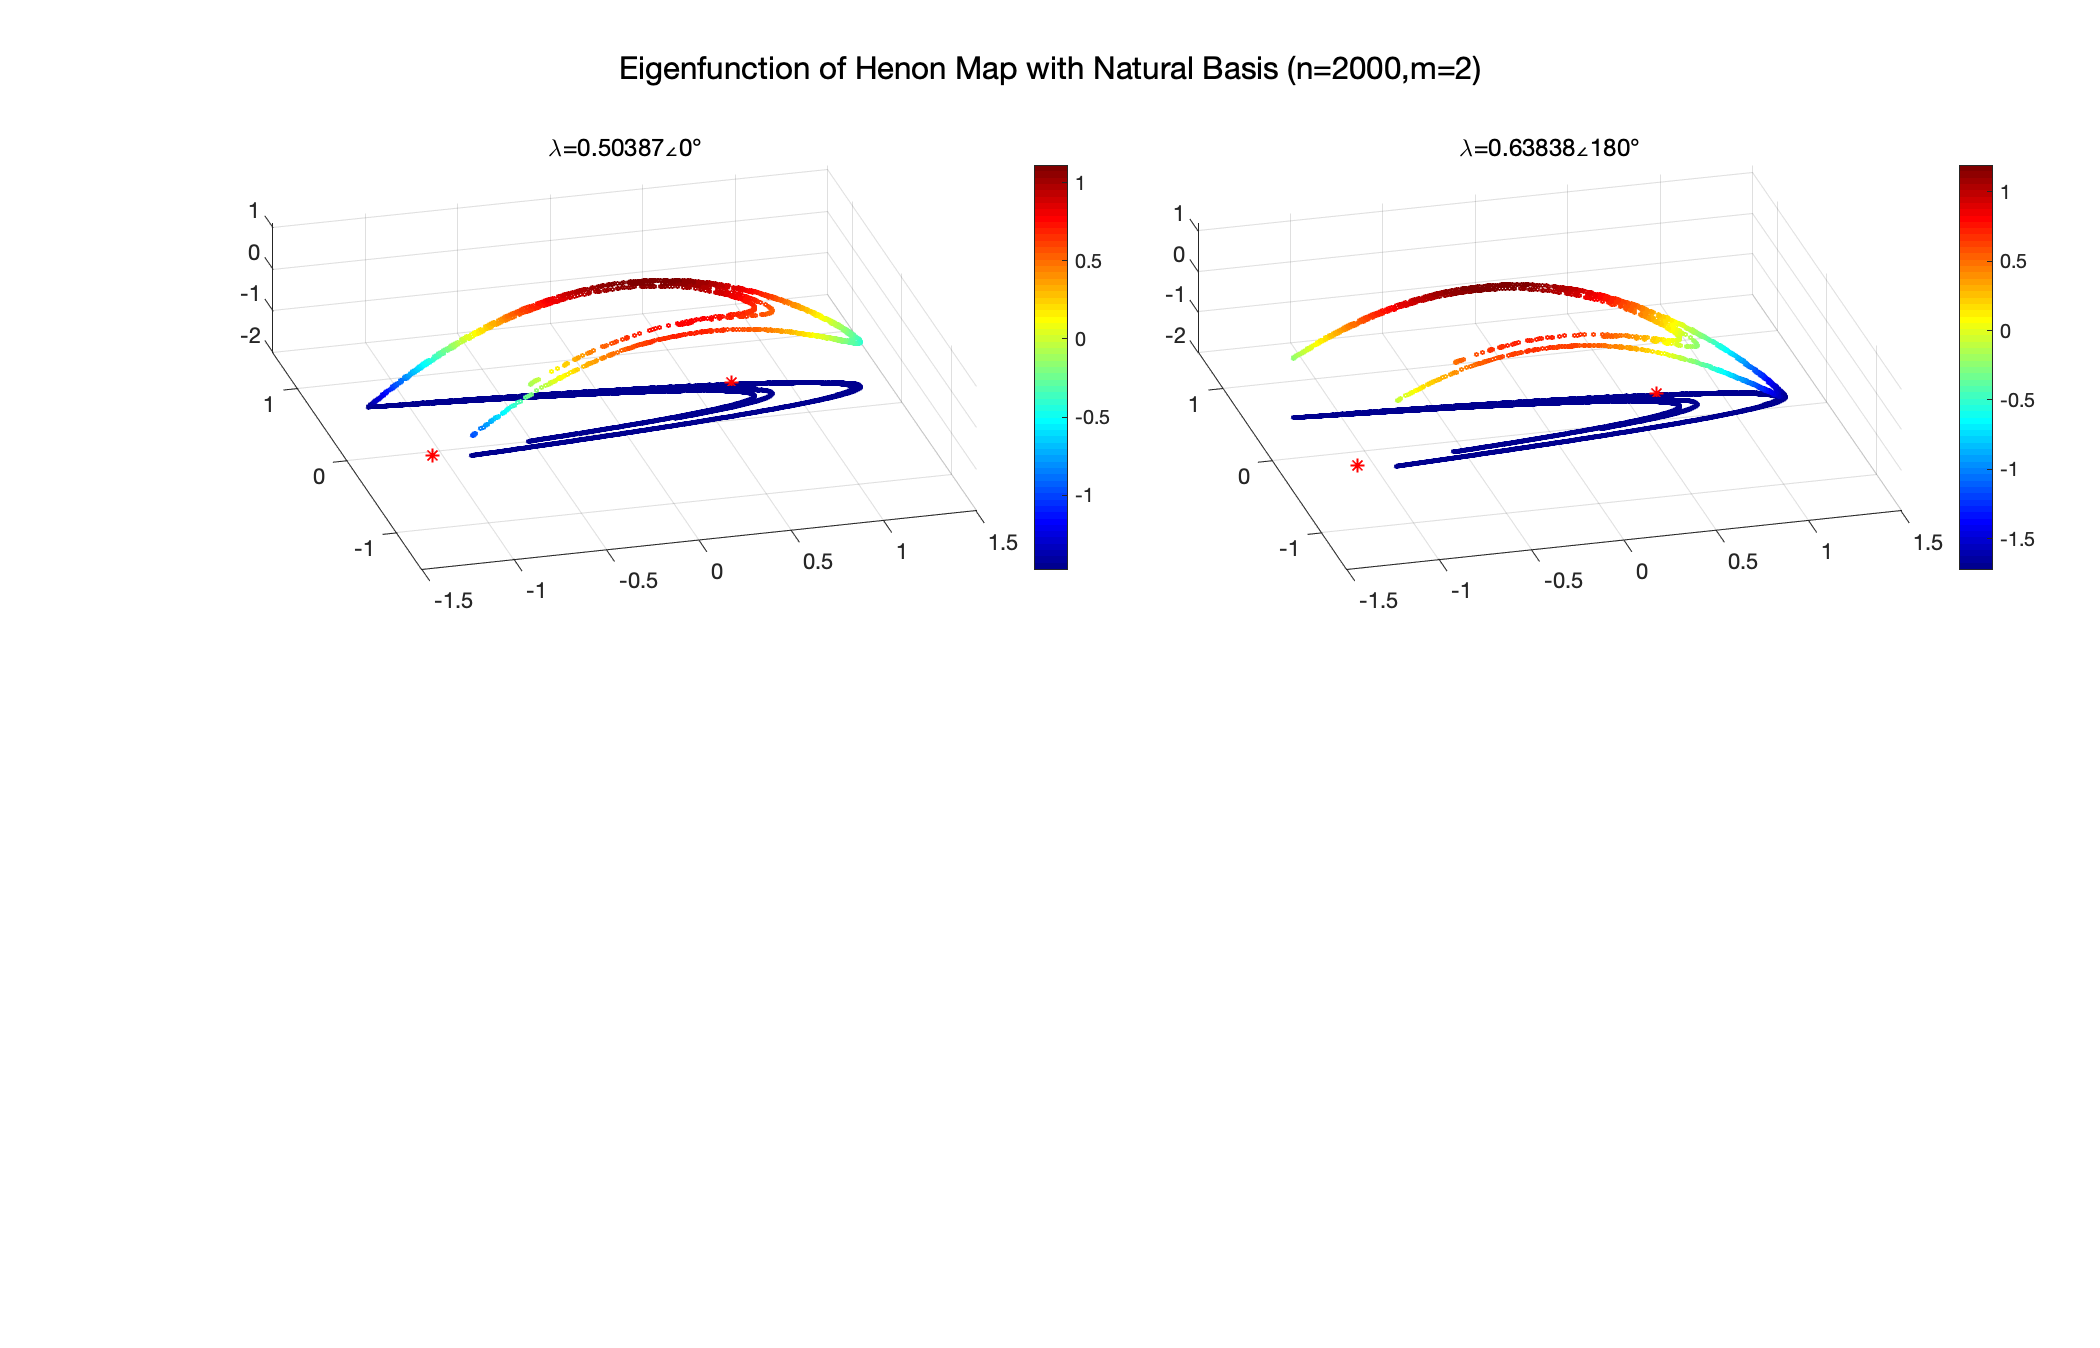
\includegraphics[scale=0.2]{henon/natural/Henon_eigen_natural_n2000m2}}
    \\
    \subfloat[m=3]{
      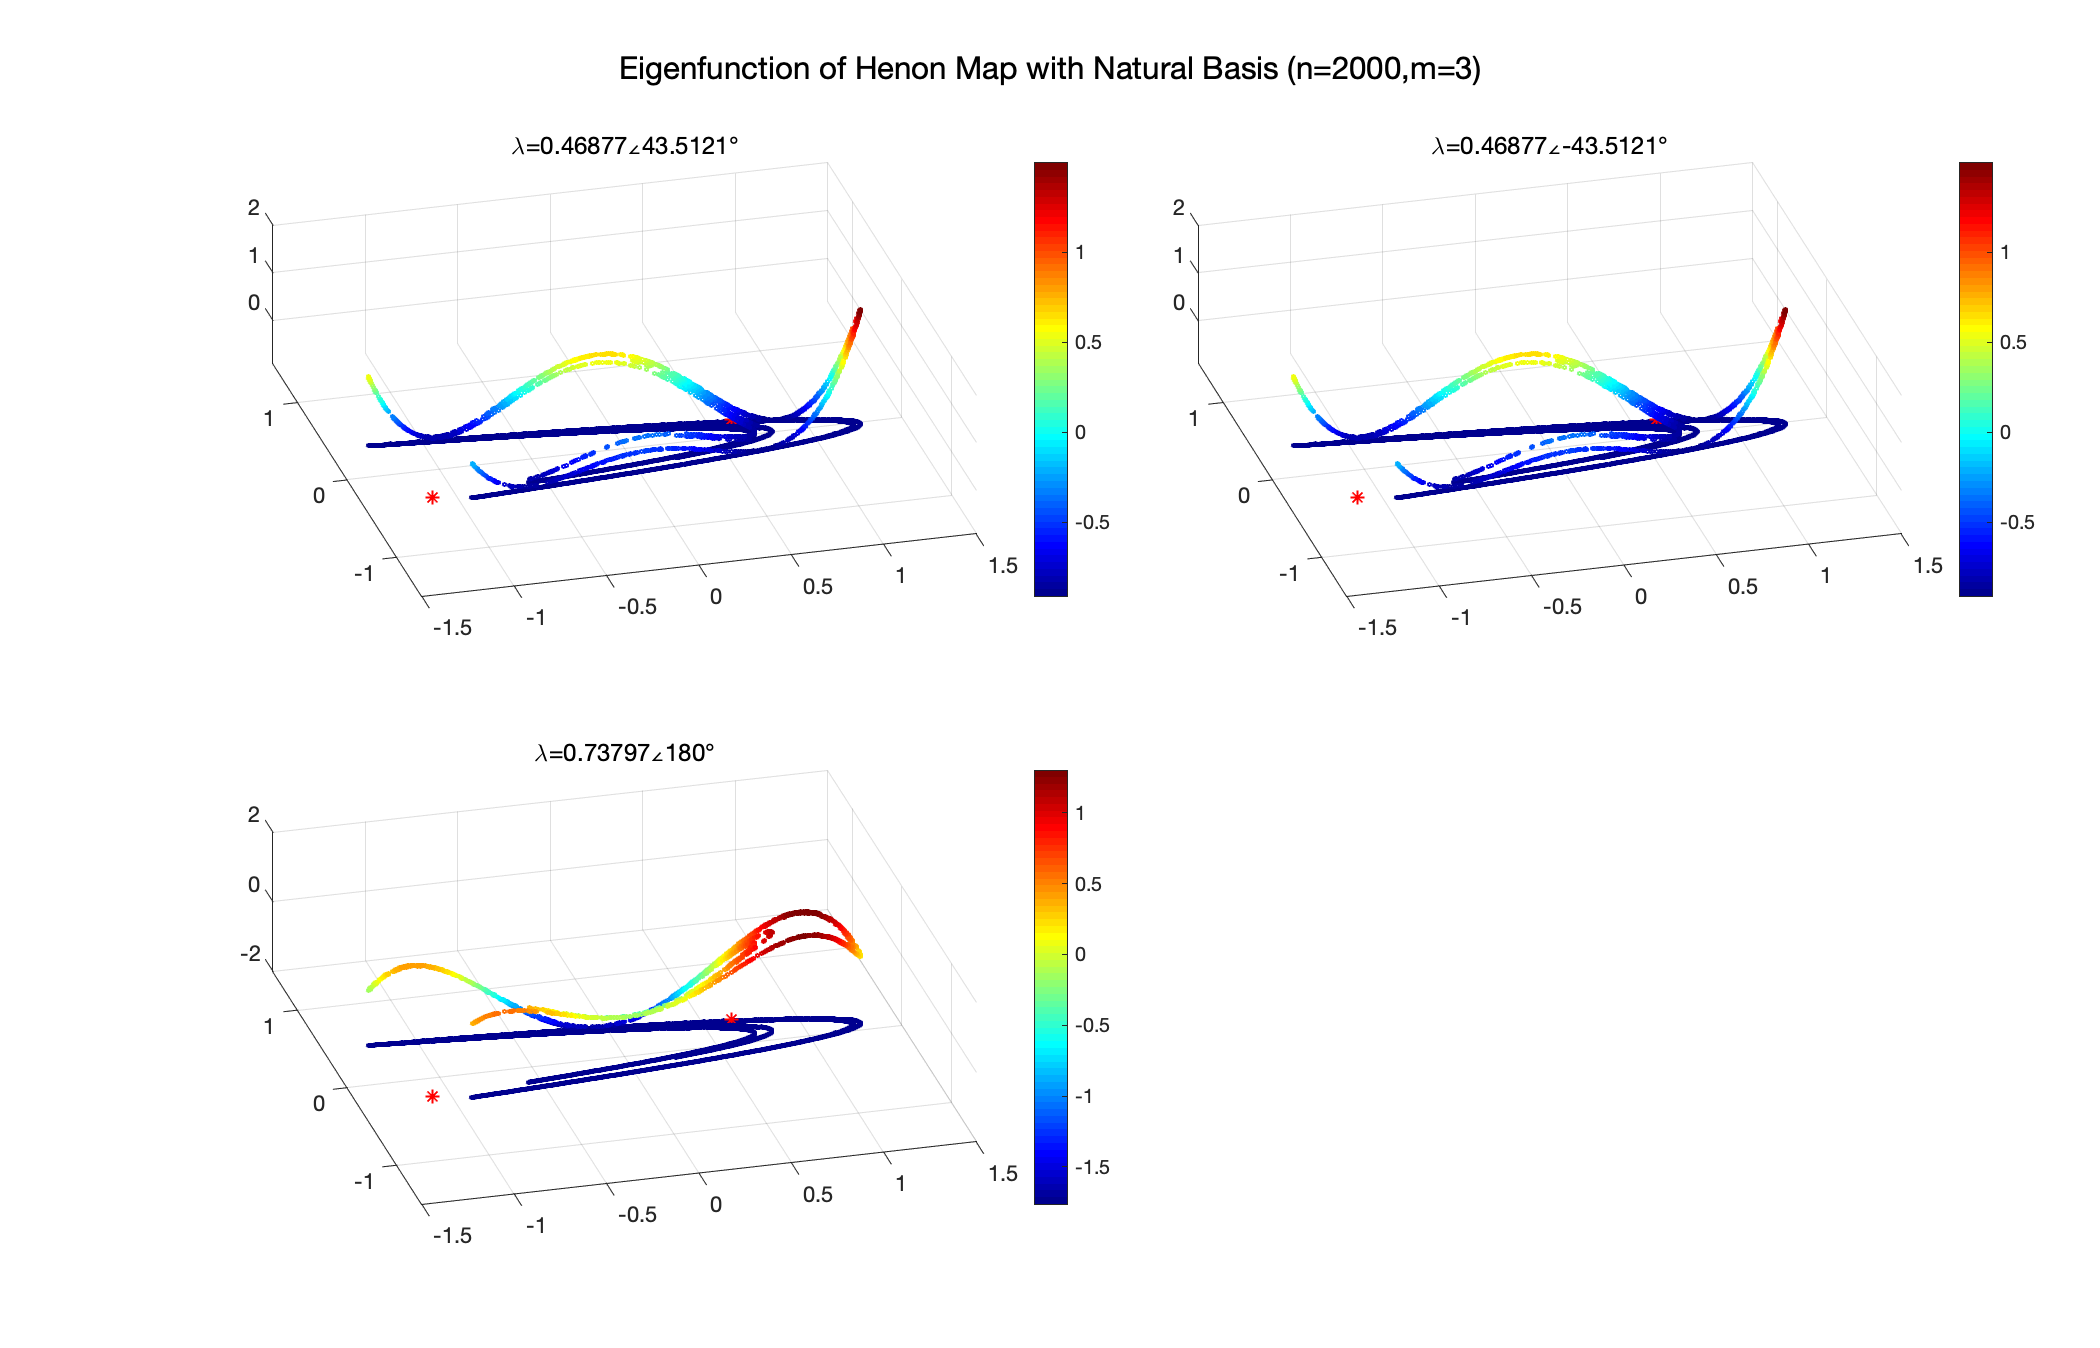
\includegraphics[scale=0.2]{henon/natural/Henon_eigen_natural_n2000m3}}
    \subfloat[m=4]{
      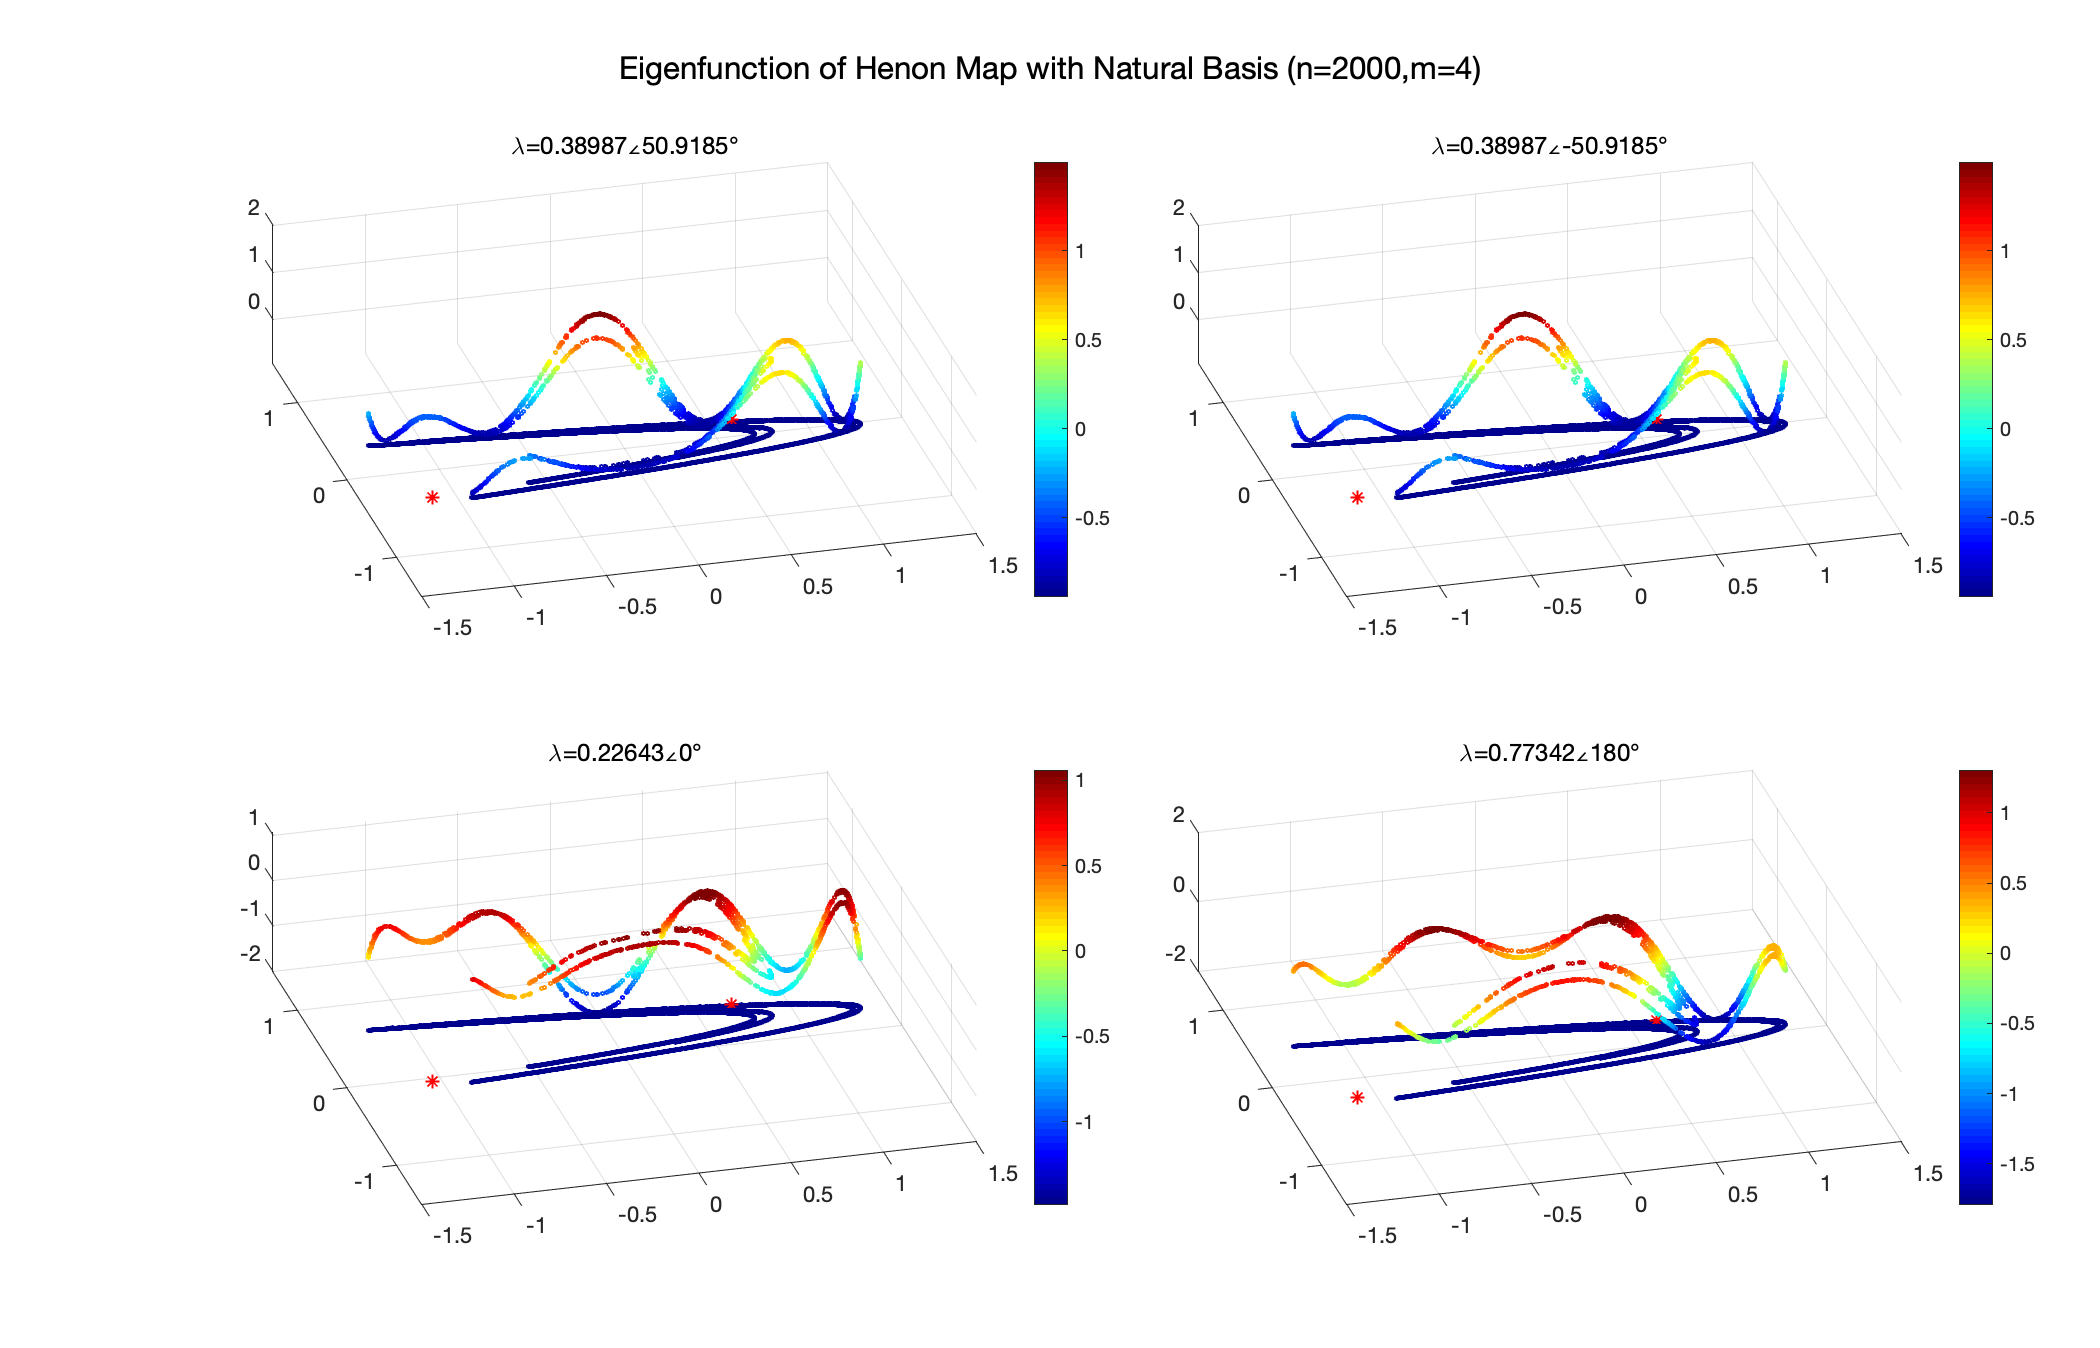
\includegraphics[scale=0.2]{henon/natural/Henon_eigen_natural_n2000m4}}
    \\
    \subfloat[m=5]{
      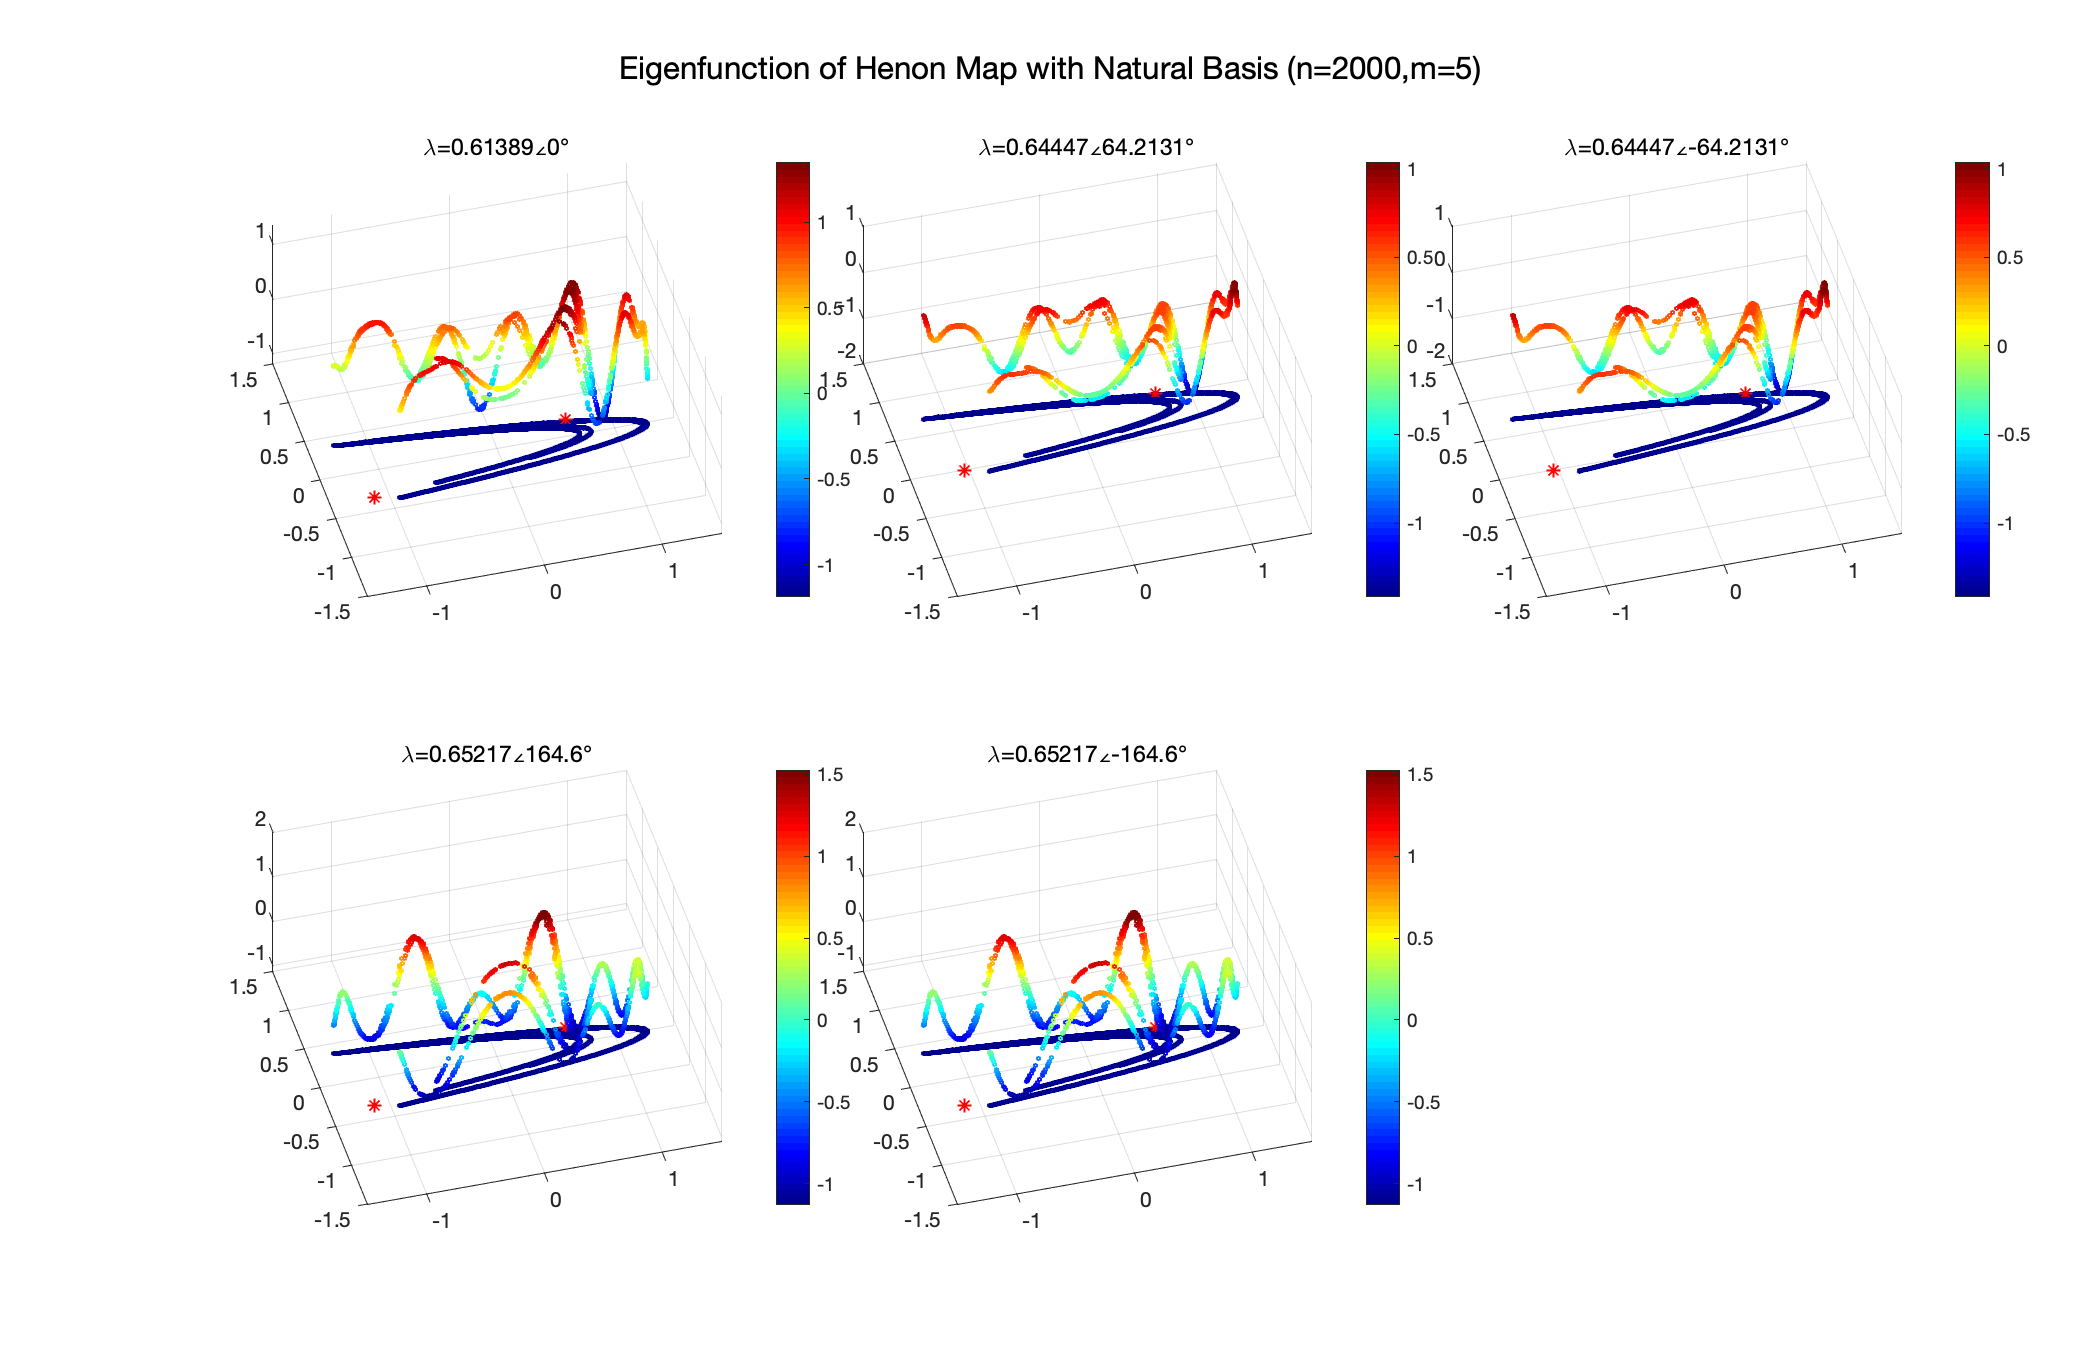
\includegraphics[scale=0.2]{henon/natural/Henon_eigen_natural_n2000m5}}
    \subfloat[m=6]{
      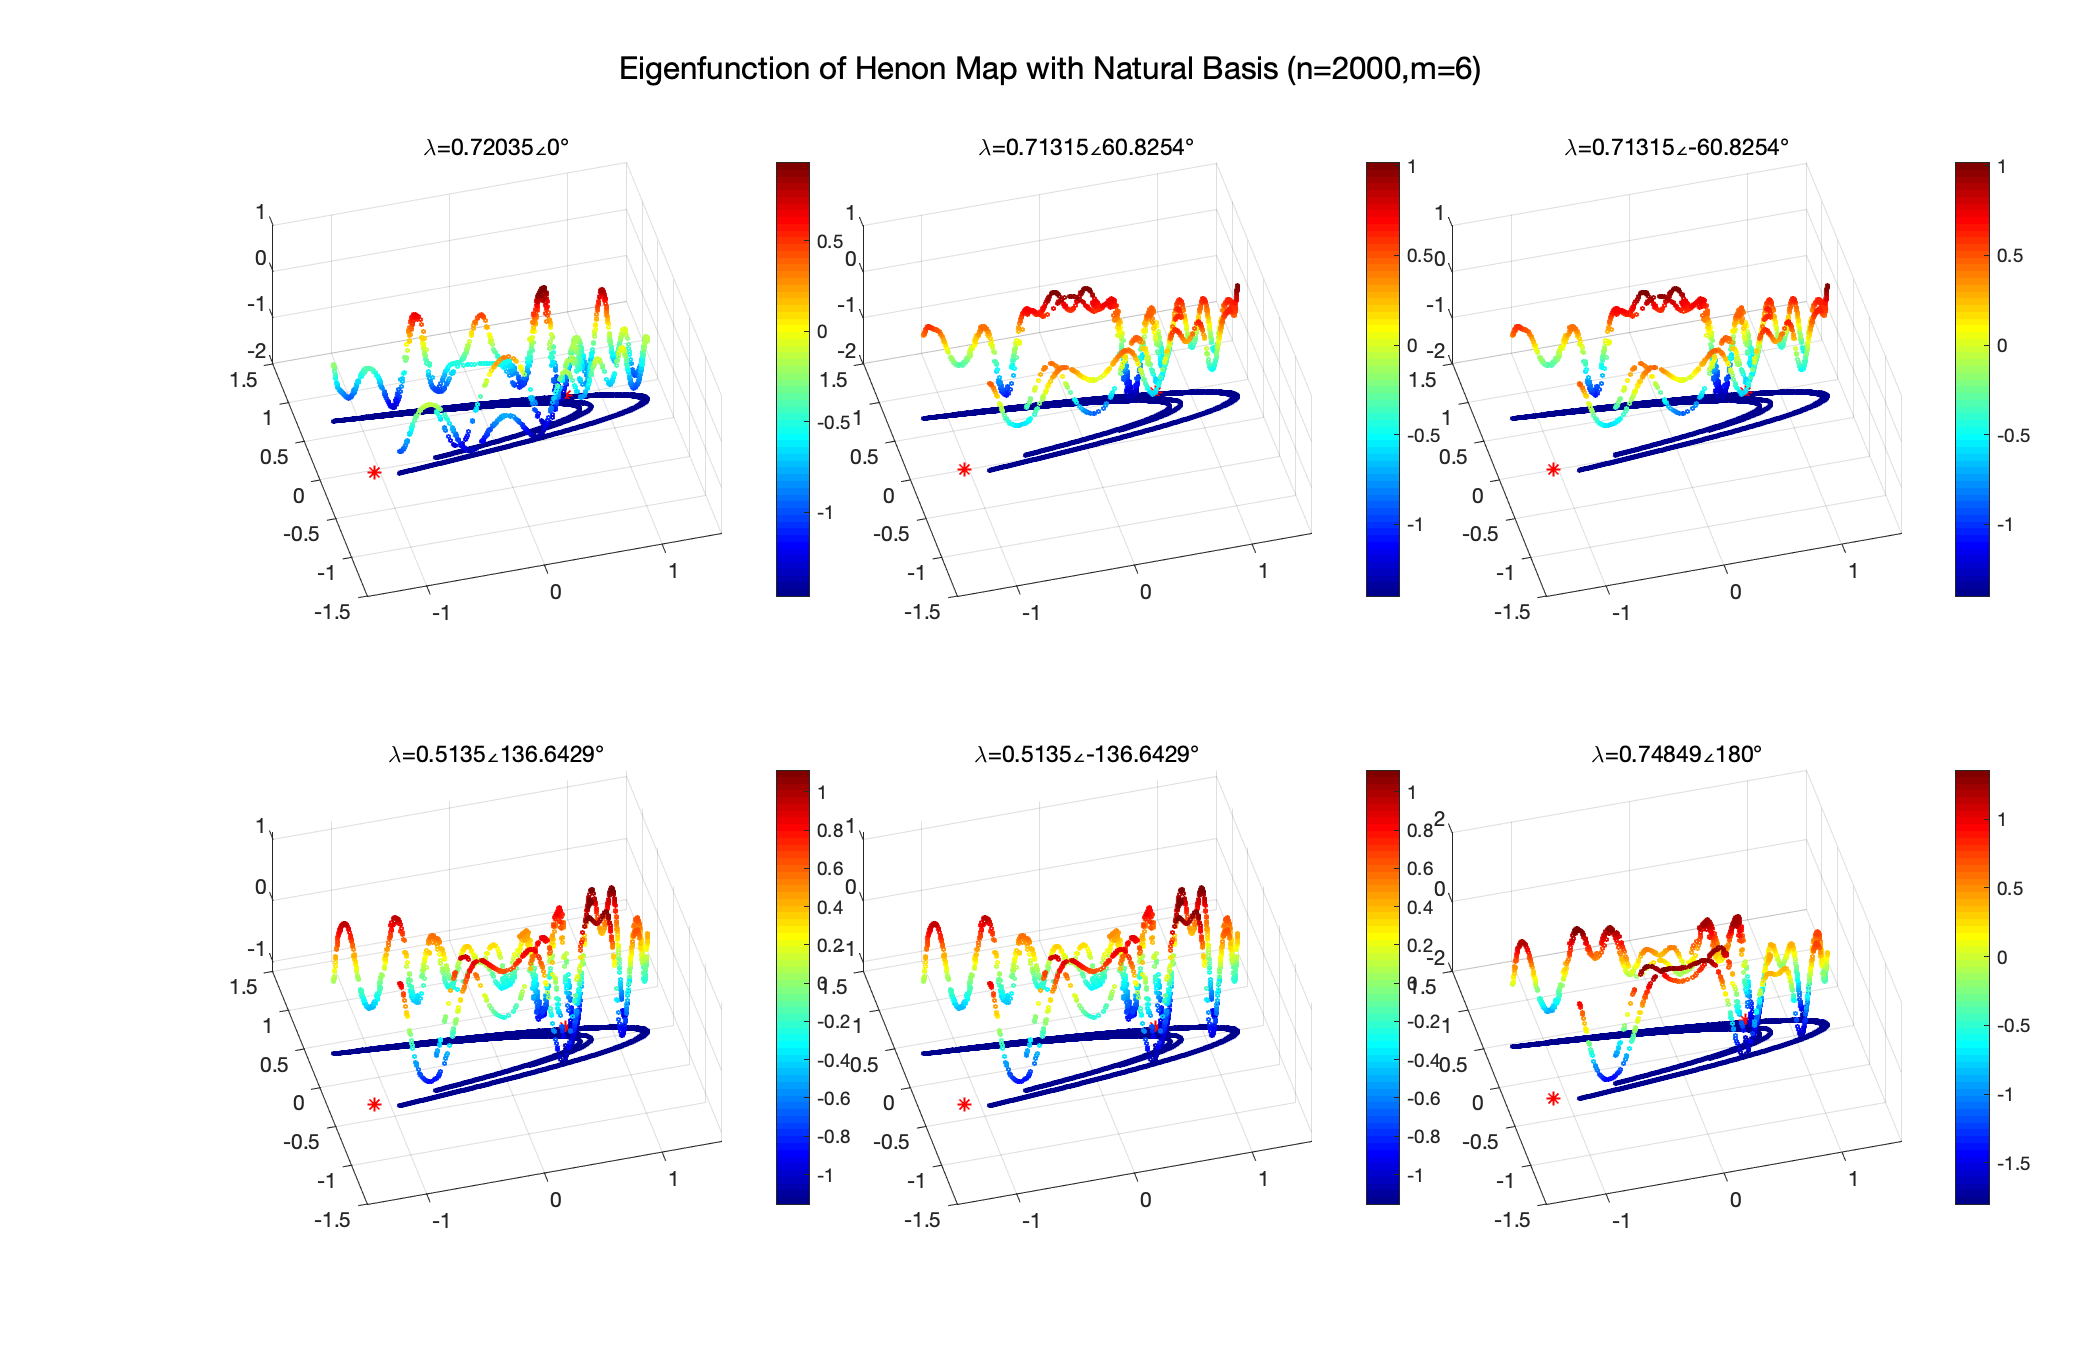
\includegraphics[scale=0.2]{henon/natural/Henon_eigen_natural_n2000m6}}
    \\
    \subfloat[m=7]{
      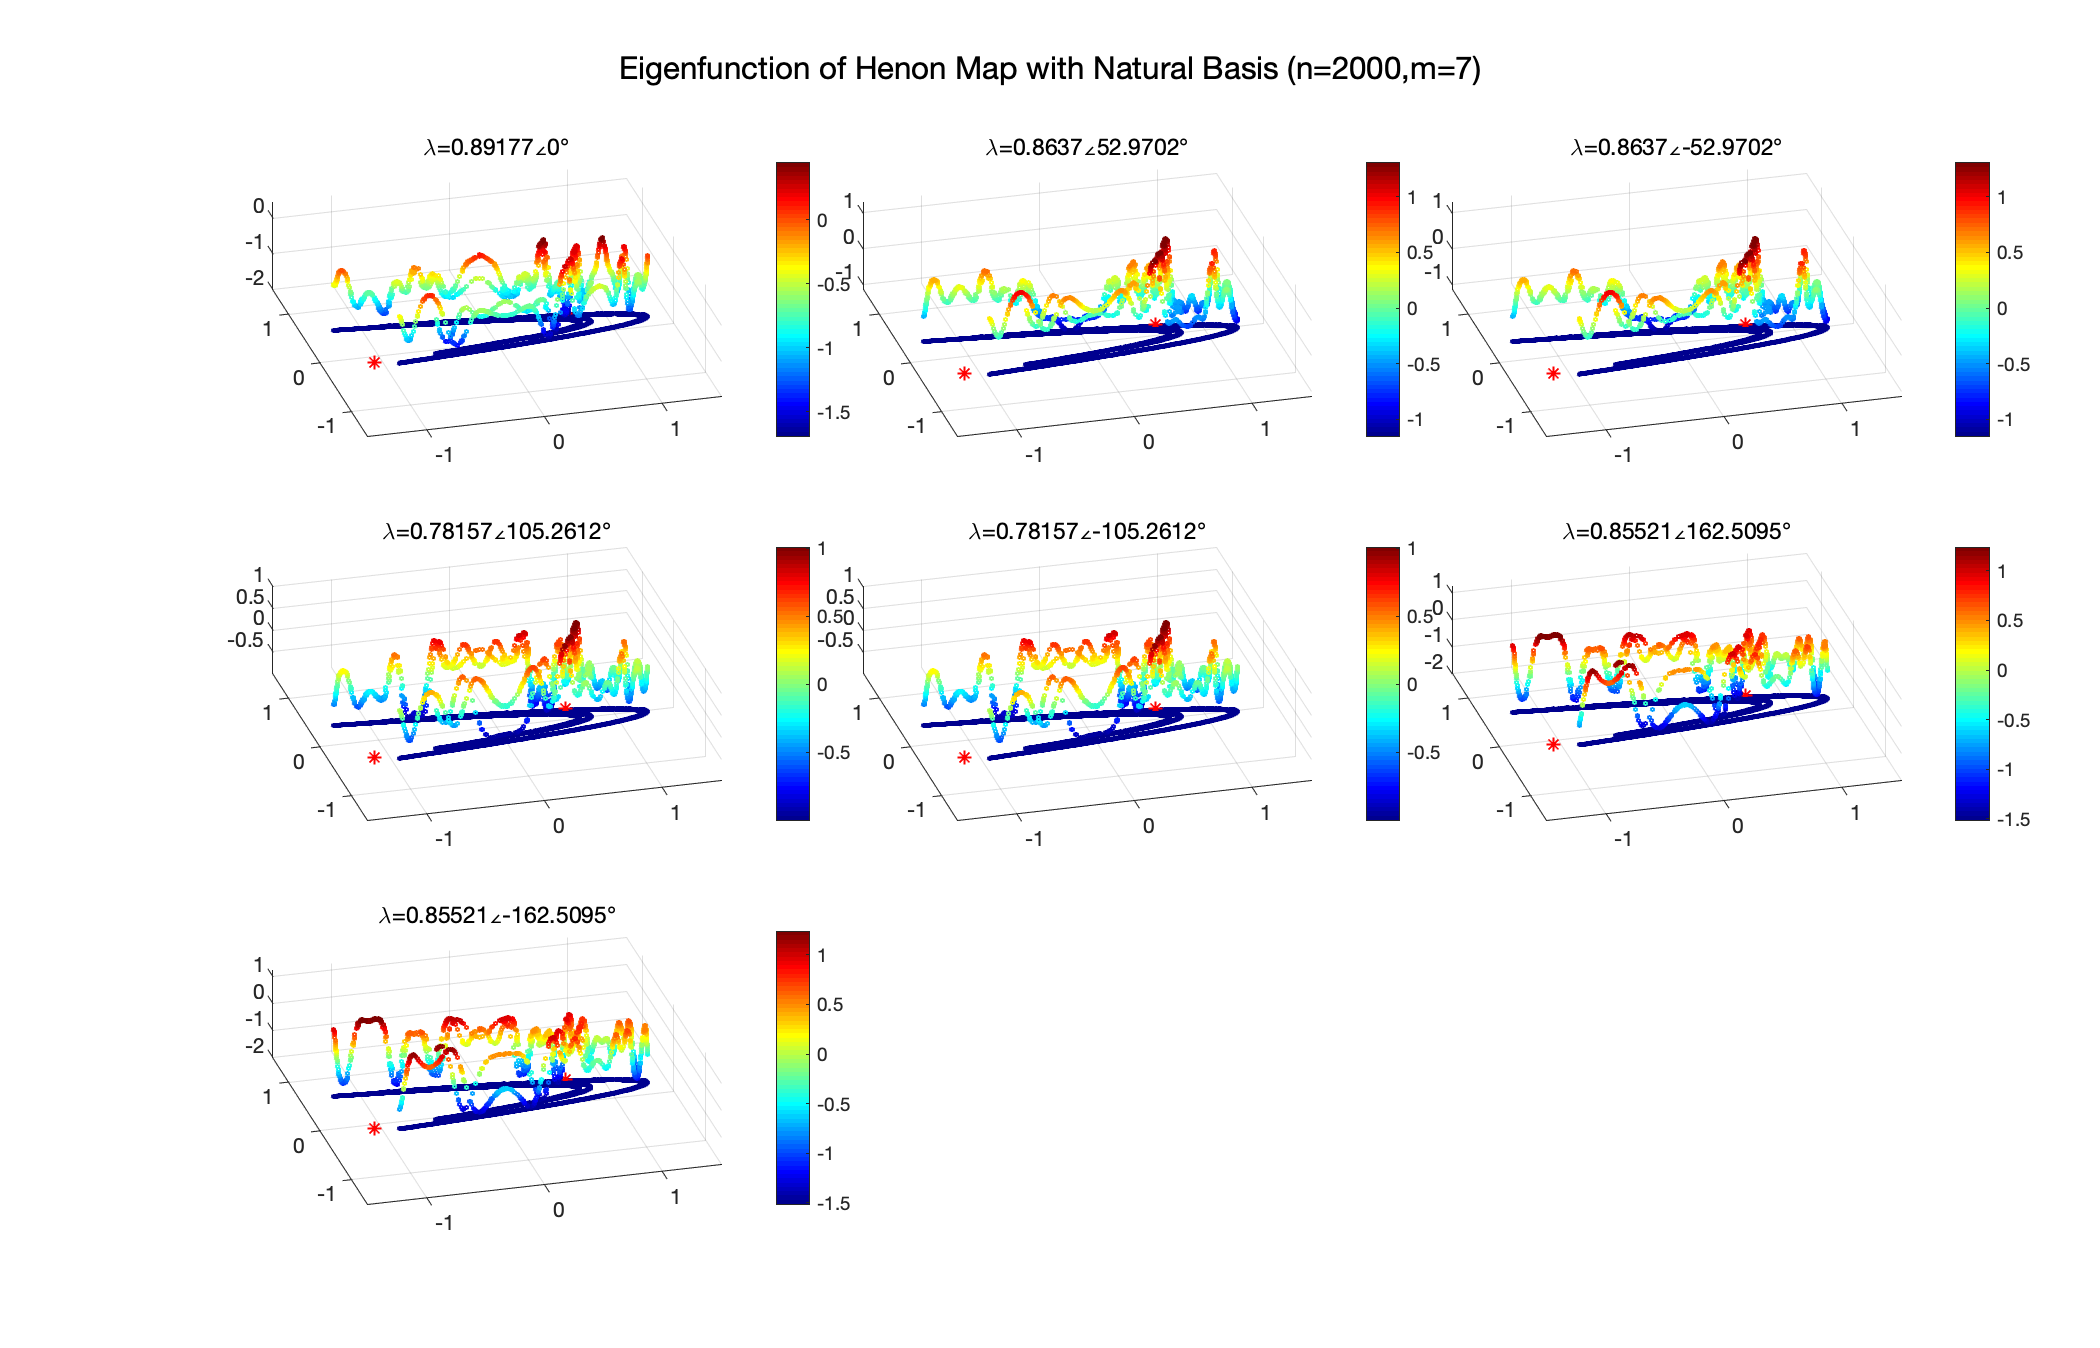
\includegraphics[scale=0.2]{henon/natural/Henon_eigen_natural_n2000m7}}
    \subfloat[m=8]{
      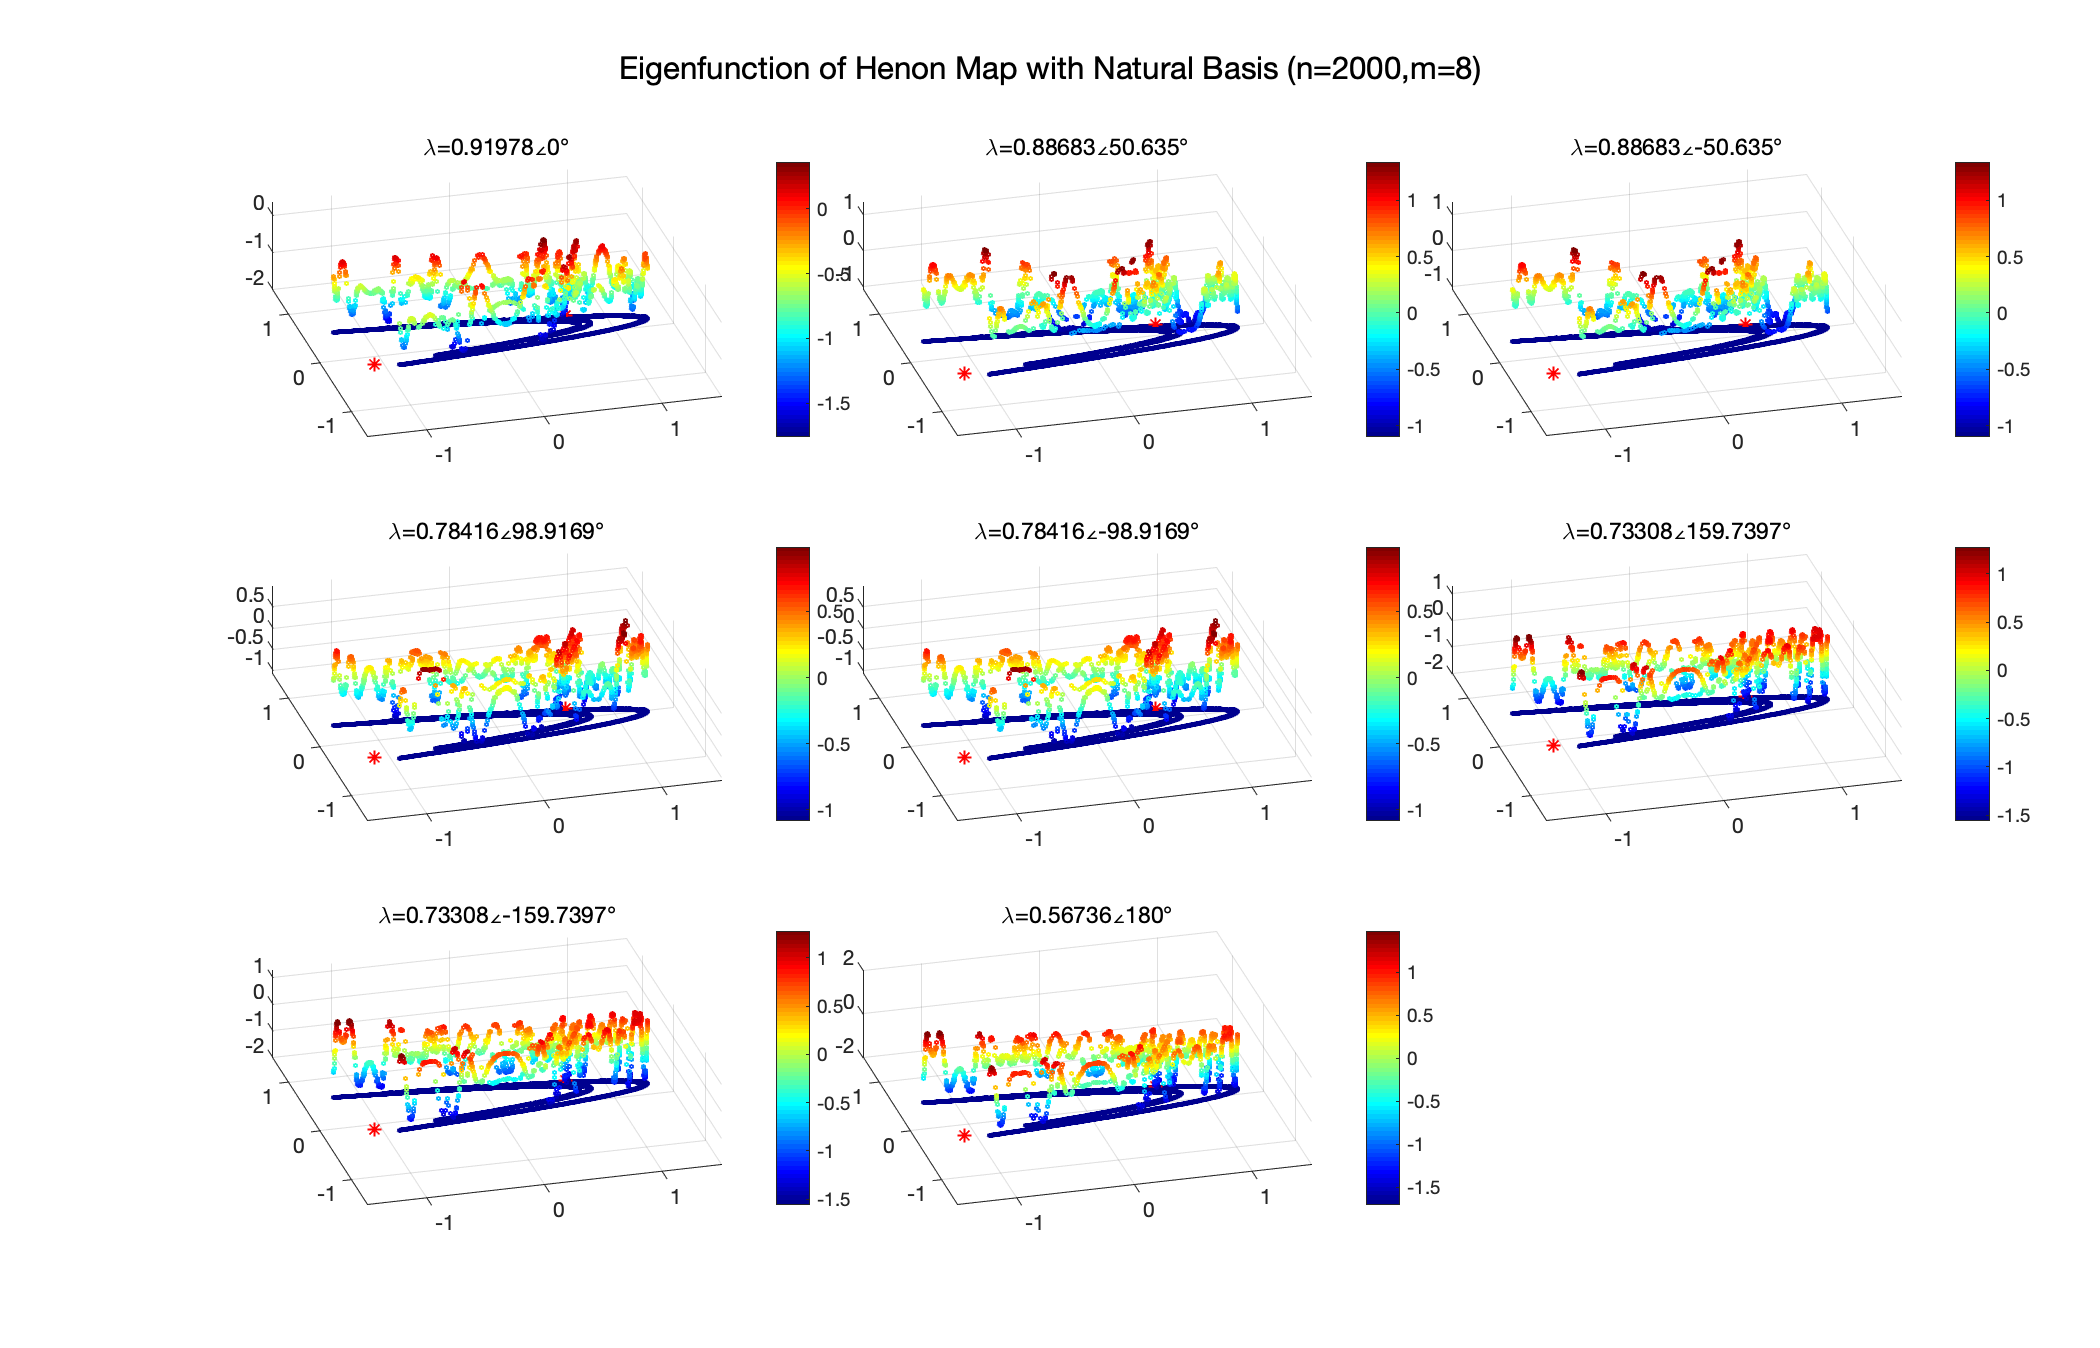
\includegraphics[scale=0.2]{henon/natural/Henon_eigen_natural_n2000m8}}
    \\
    \caption[埃农映射自然基函数不同基函数数量下的本征函数]{埃农映射自然基函数不同基函数数量下的本征函数($n=2000$):图中颜色值及高度值均表示本征函数值的大小,且其在xy平面的投影为二维吸引子域}\label{fig:Henon_eigen_natural_n2000m1}
\end{figure}

当$m=1,2,3,4,5,6,7,8,9$时,我们每个基函数仅取一个本征函数图像,观察随着基函数的增加,本征函数的图像如何变化,如图\ref{fig:Henon_eigen_natural_n2000}。

\begin{figure}
	\centering
	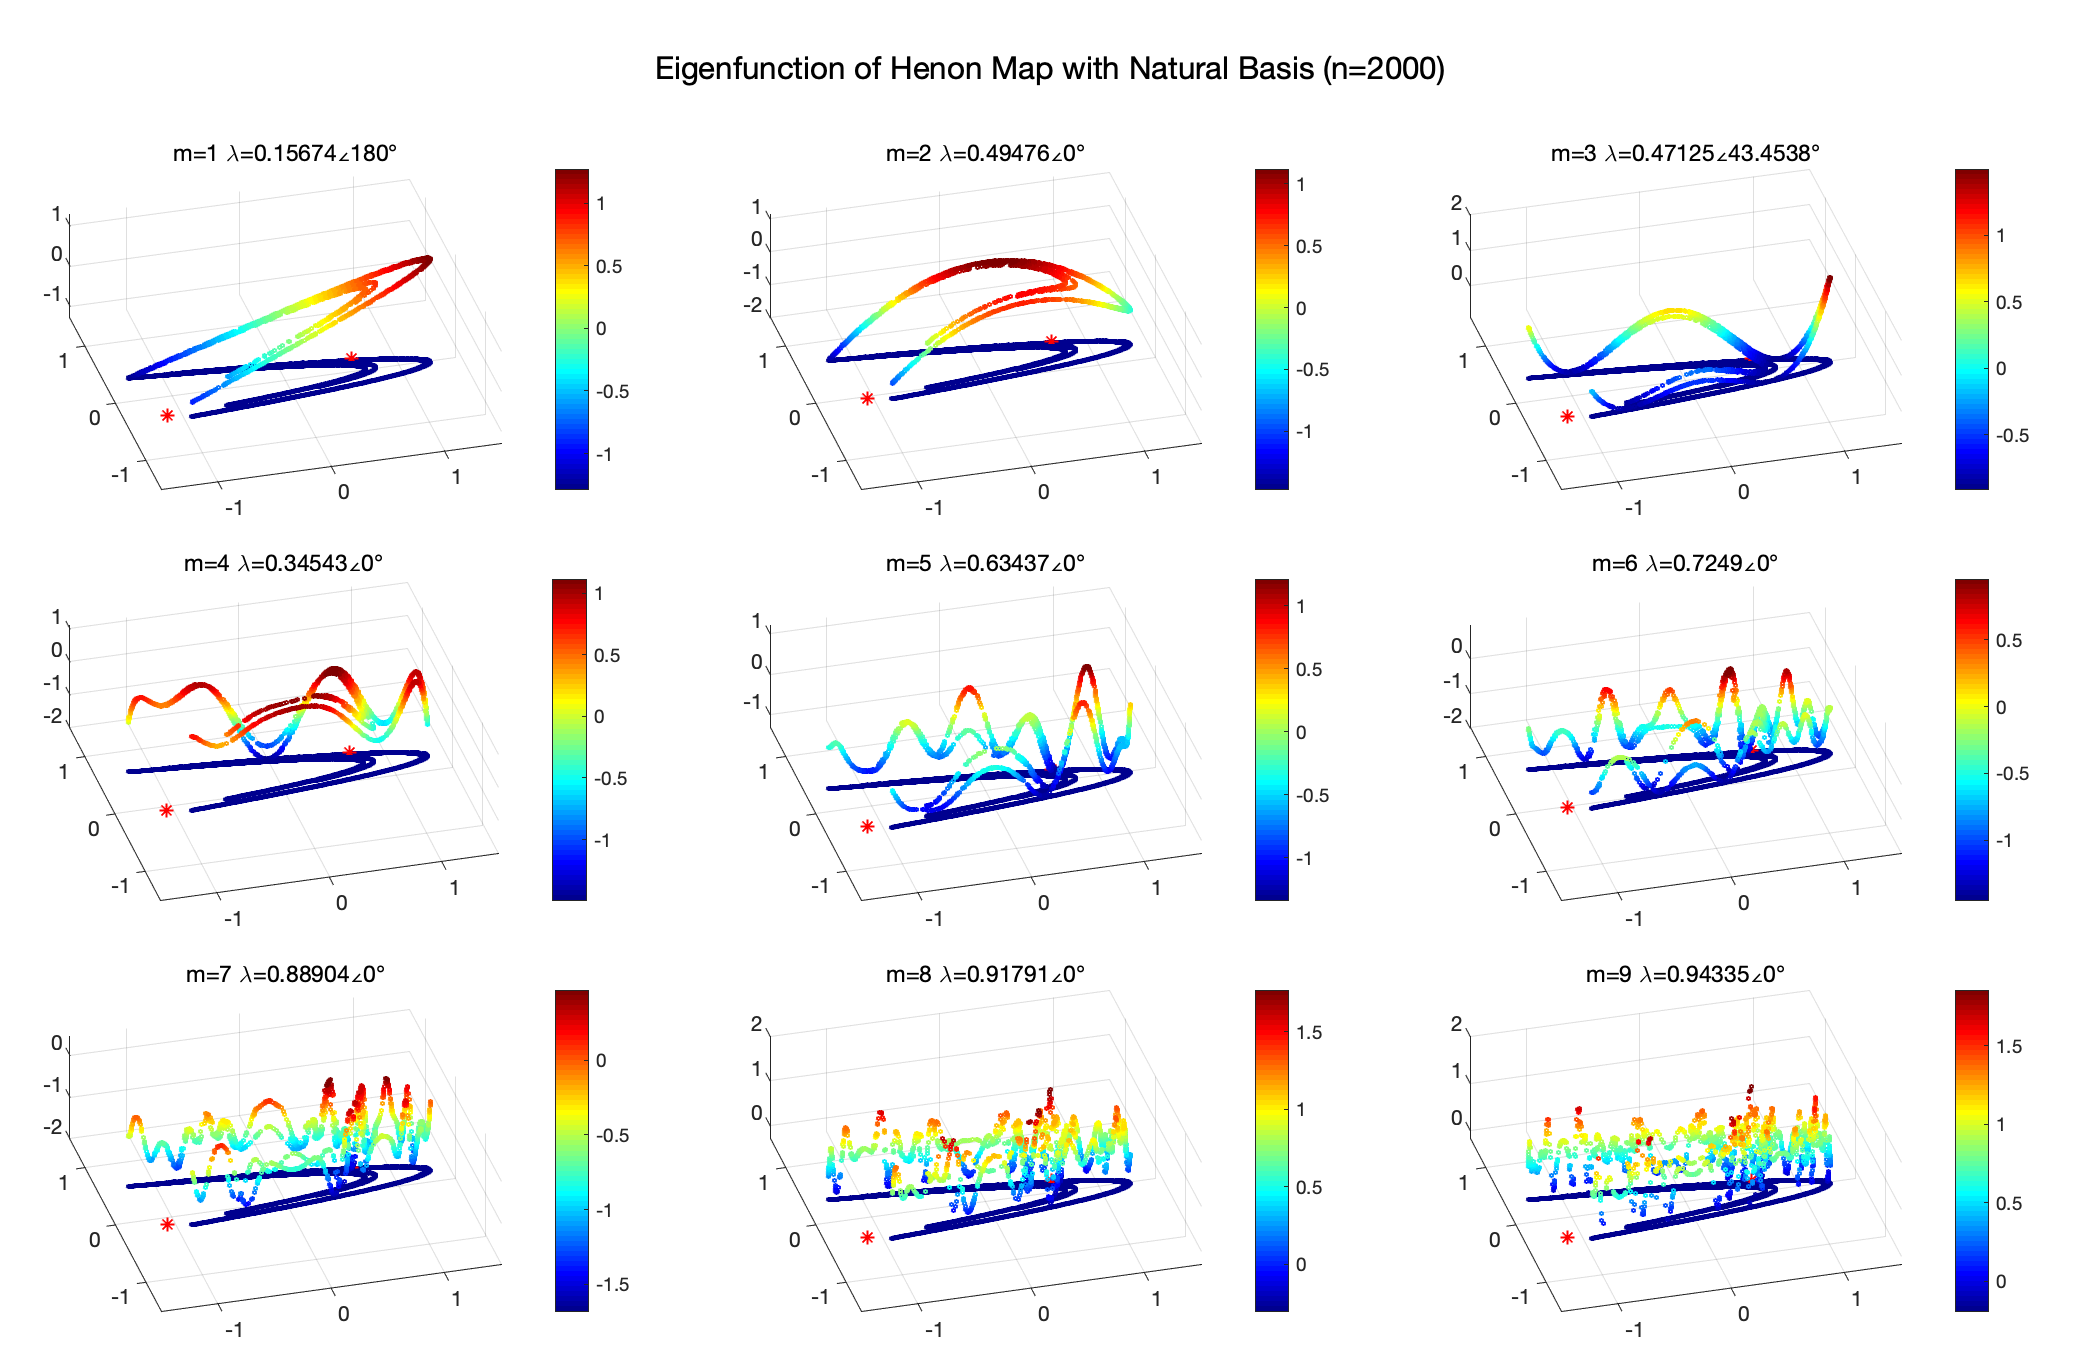
\includegraphics[scale=0.4]{henon/natural/Henon_eigen_natural_n2000}
    \caption{埃农映射自然基函数不同基函数数量下的本征函数($n=2000$):图中颜色值及高度值均表示本征函数值的大小,且其在xy平面的投影为二维吸引子域}\label{fig:Henon_eigen_natural_n2000}
\end{figure}

结合图\ref{fig:Henon_eigen_natural_n2000m1}与图\ref{fig:Henon_eigen_natural_n2000},我们观察到,随着基函数数量的增加,本征函数图像增加了一些极值点,但并未丢失之前的极值点,若我们可以证明这些极值点属于埃农映射不同层次的边界点,我们便可以得出和一维映射一致的结论:Koopman算符的本征函数的极值点反映了埃农映射的边界点,且随着基函数数量的增加,能区分更多层次的边界点。

\subsection{Koopman算符对埃农映射的相空间吸引子划分}

在埃农映射的本征函数图像中,我们可以发现一些关键的本征函数的极值点,若能证明这些极值点对应埃农映射的边界点,我们便可以得出和一维映射一致的结论:Koopman算符的本征函数极值点反映了动力学系统的边界点。埃农映射的边界点可以通过稳定流型和不稳定流型的同宿切面得到\cite{d1990topology,giovannini1992generating,grassberger1989symbolic},且这种划分的拓扑性质具有较高的准确性\cite{d1990topology},如表\ref{tab:henon_boundary}。
\begin{table}[]
    \centering
    \begin{tabular}{|c|c|c|}
    \hline
        & 横坐标x & 纵坐标y  \\ \hline
    1   & 0.7021 & -0.0044 \\ \hline
    2   & 0.7986 & 0.0019  \\ \hline
    3   & 1.2307 & -0.0249 \\ \hline
    4   & 1.2717 & -0.0205 \\ \hline
    \end{tabular}
    \caption{埃农映射的边界点}\label{tab:henon_boundary}
\end{table}
我们将埃农映射的边界点与吸引子画在一起,如图\ref{fig:henon_boundary},观察其位置发现,这些点都处于埃农映射吸引子最主要的弯折区域,由于埃农映射的吸引子是一个分形结构,因此在弯折区域存在4个边界点。
\begin{figure}
	\centering
	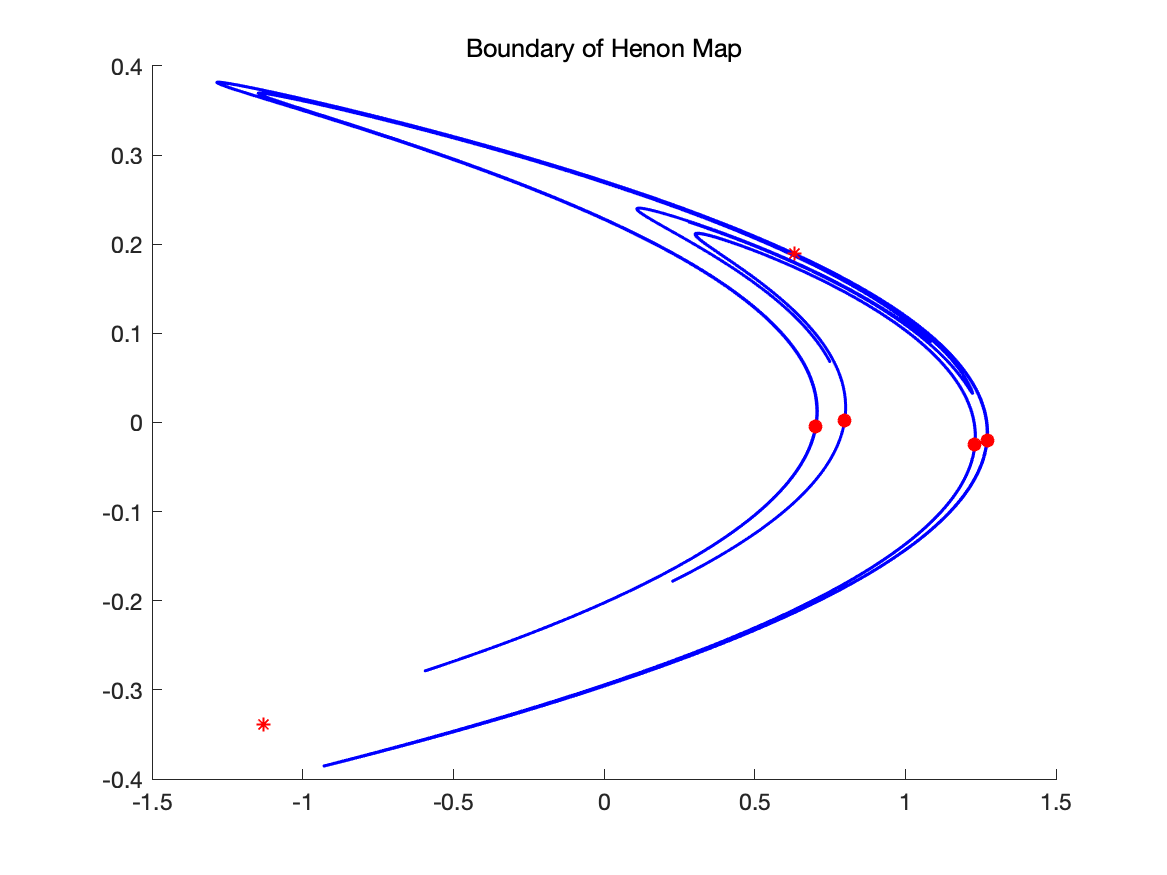
\includegraphics[scale=0.6]{henon/attractors/Henon_boundary}
    \caption[埃农映射的边界点]{埃农映射的边界点:蓝色的点表示埃农映射的吸引子,红色的星点表示埃农映射的不动点,红色的实心点表示埃农映射的边界点}\label{fig:henon_boundary}
\end{figure}
为了能寻找到其他层次的边界点,我们对埃农映射的四个边界点进行正向演化得到其像点,反向演化得到其原像点,如图\ref{fig:Henon_boundary_forward},我们将正向演化及其次数用正数标注在图中,将反向演化及其次数用负数标注在图中,$0$表示最原始的四个边界点。在之前的讨论中,我们称边界点的原像点为其他层次的边界点,在此处我们同样这样定义。我们对比本征函数图像的极值点及埃农映射的边界点。
\begin{figure}
    \centering
    \subfloat[正向迭代]{
      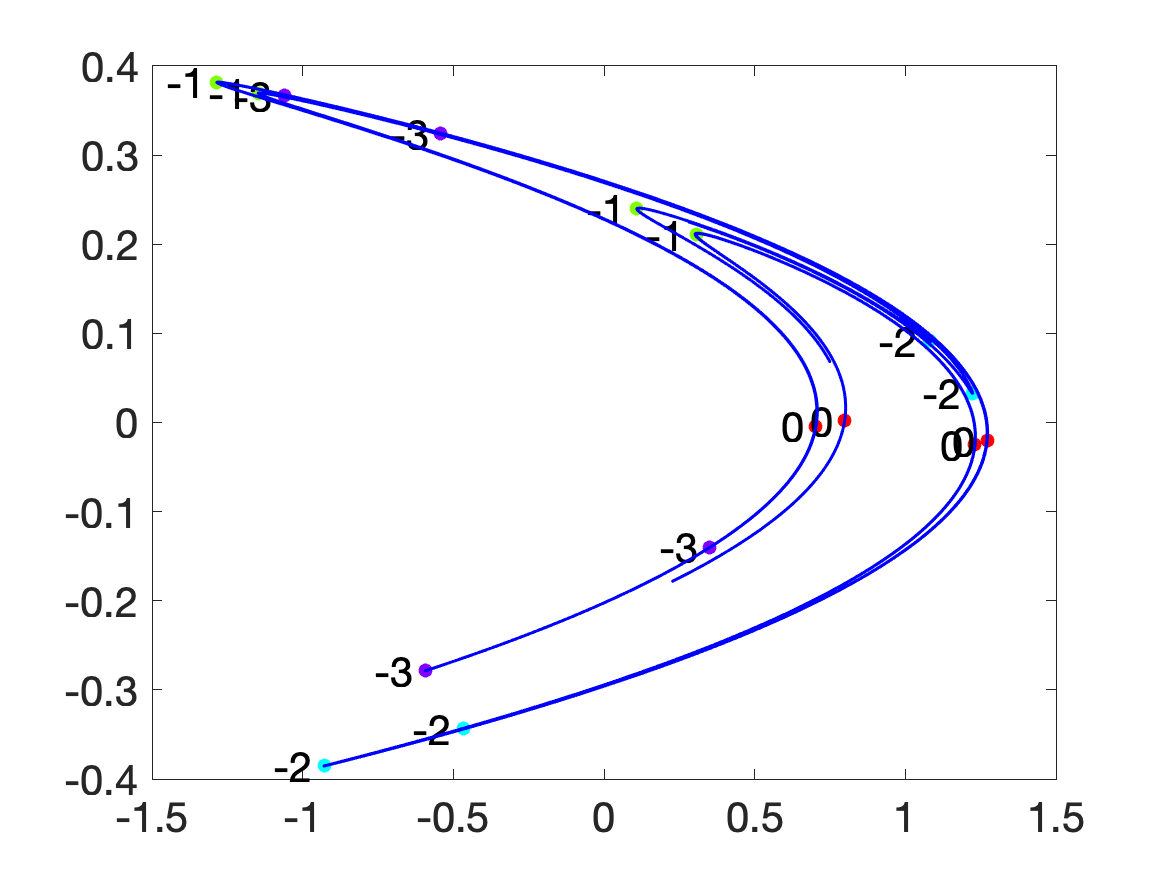
\includegraphics[scale=0.4]{henon/attractors/Henon_boundary_forward}}
    \subfloat[反向迭代]{
      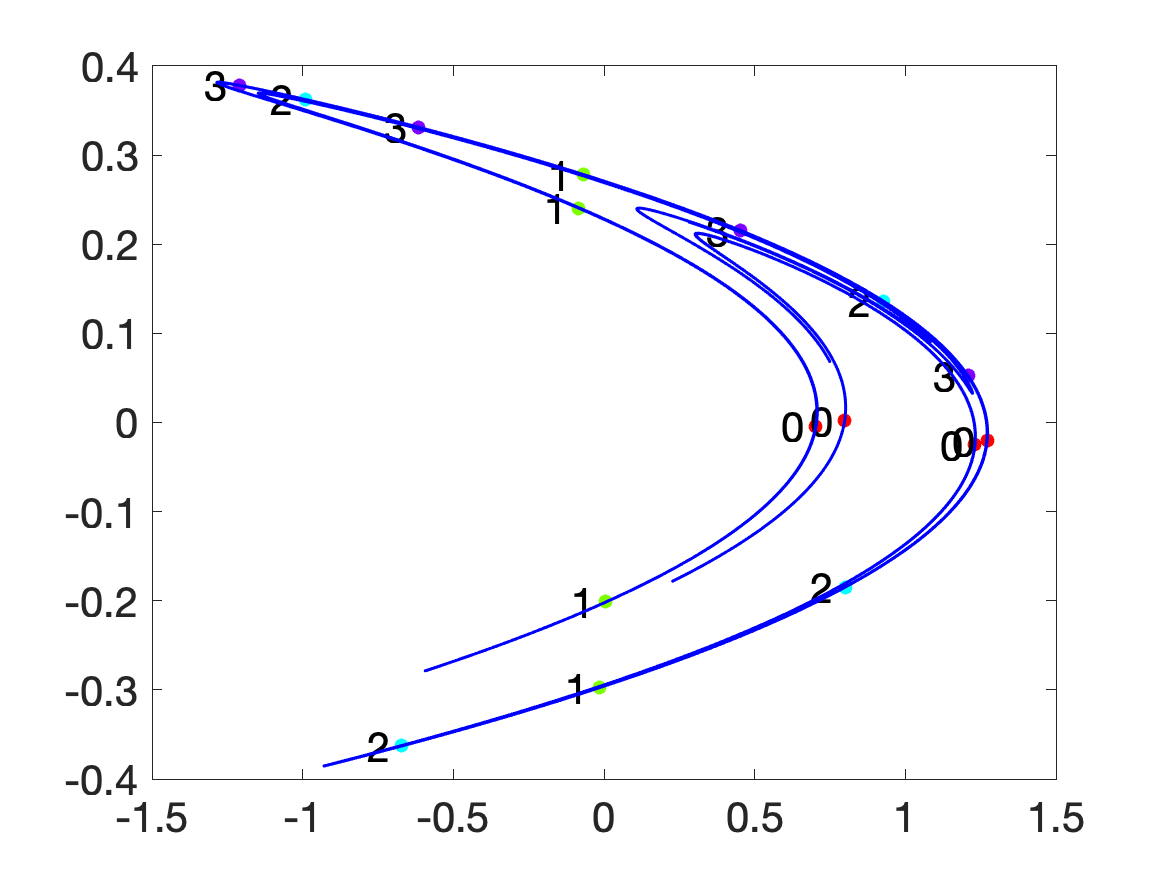
\includegraphics[scale=0.4]{henon/attractors/Henon_boundary_reverse}}
    \caption{埃农映射的边界点及其像点、原像点}\label{fig:Henon_boundary_forward}
\end{figure}

我们选取自然基函数,并取演化格点数量$n=2000$,函数格点数量$m=1,2,3,4,5,6,7,8$,分别作本征函数图像,并将边界点的位置标出,如图。
\begin{figure}
    \centering
    \subfloat[m=1]{
      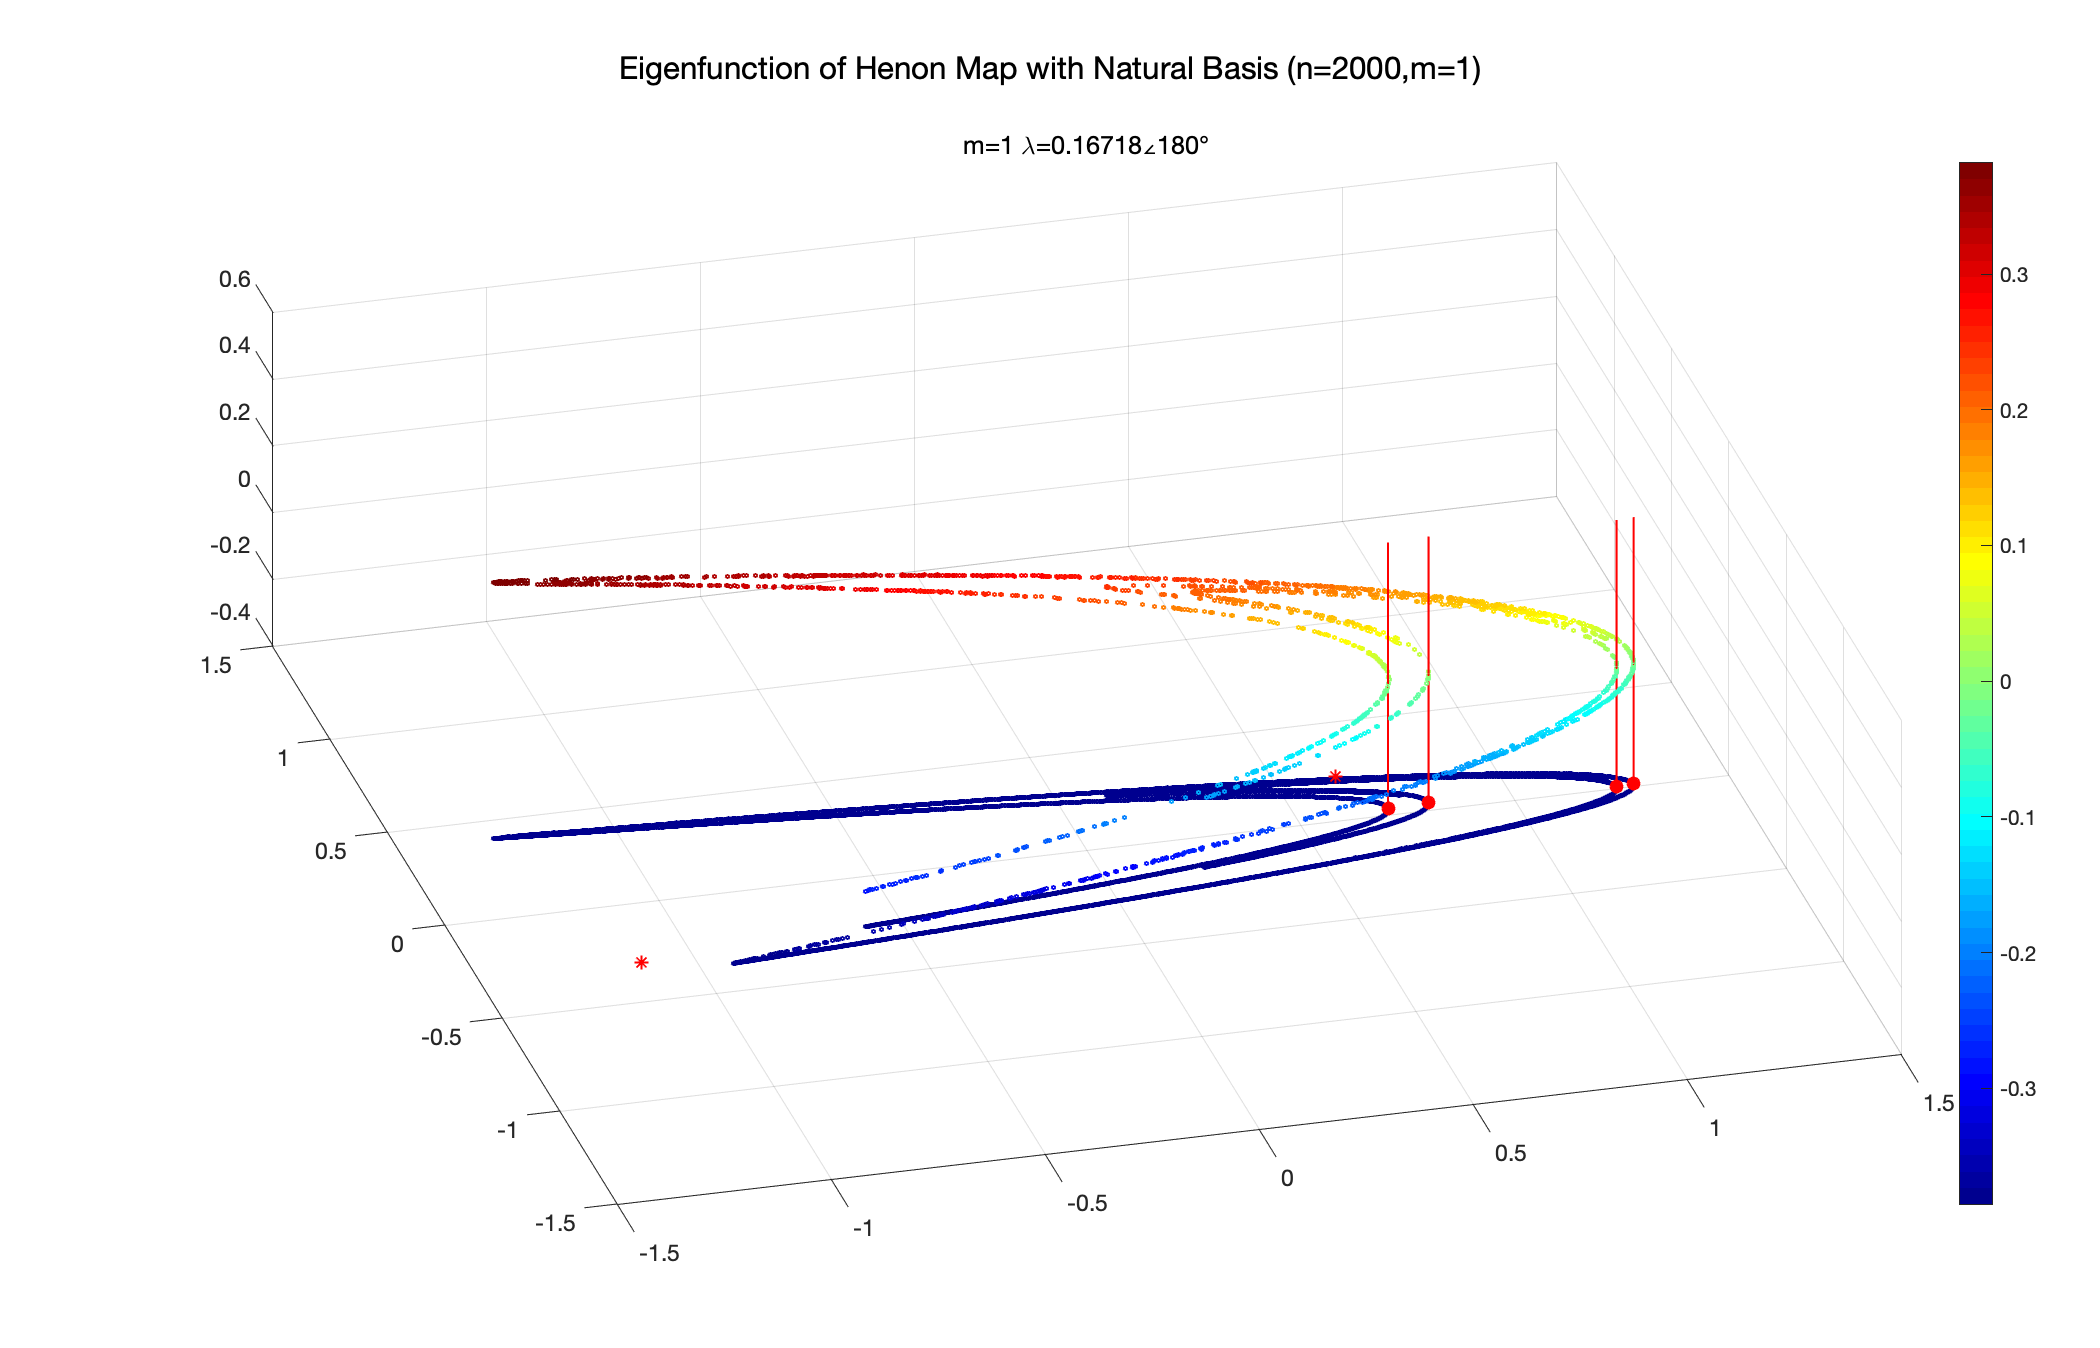
\includegraphics[scale=0.2]{henon/attractors/Henon_eigen_natural_attr_n2000m1}}
    \subfloat[m=2]{
      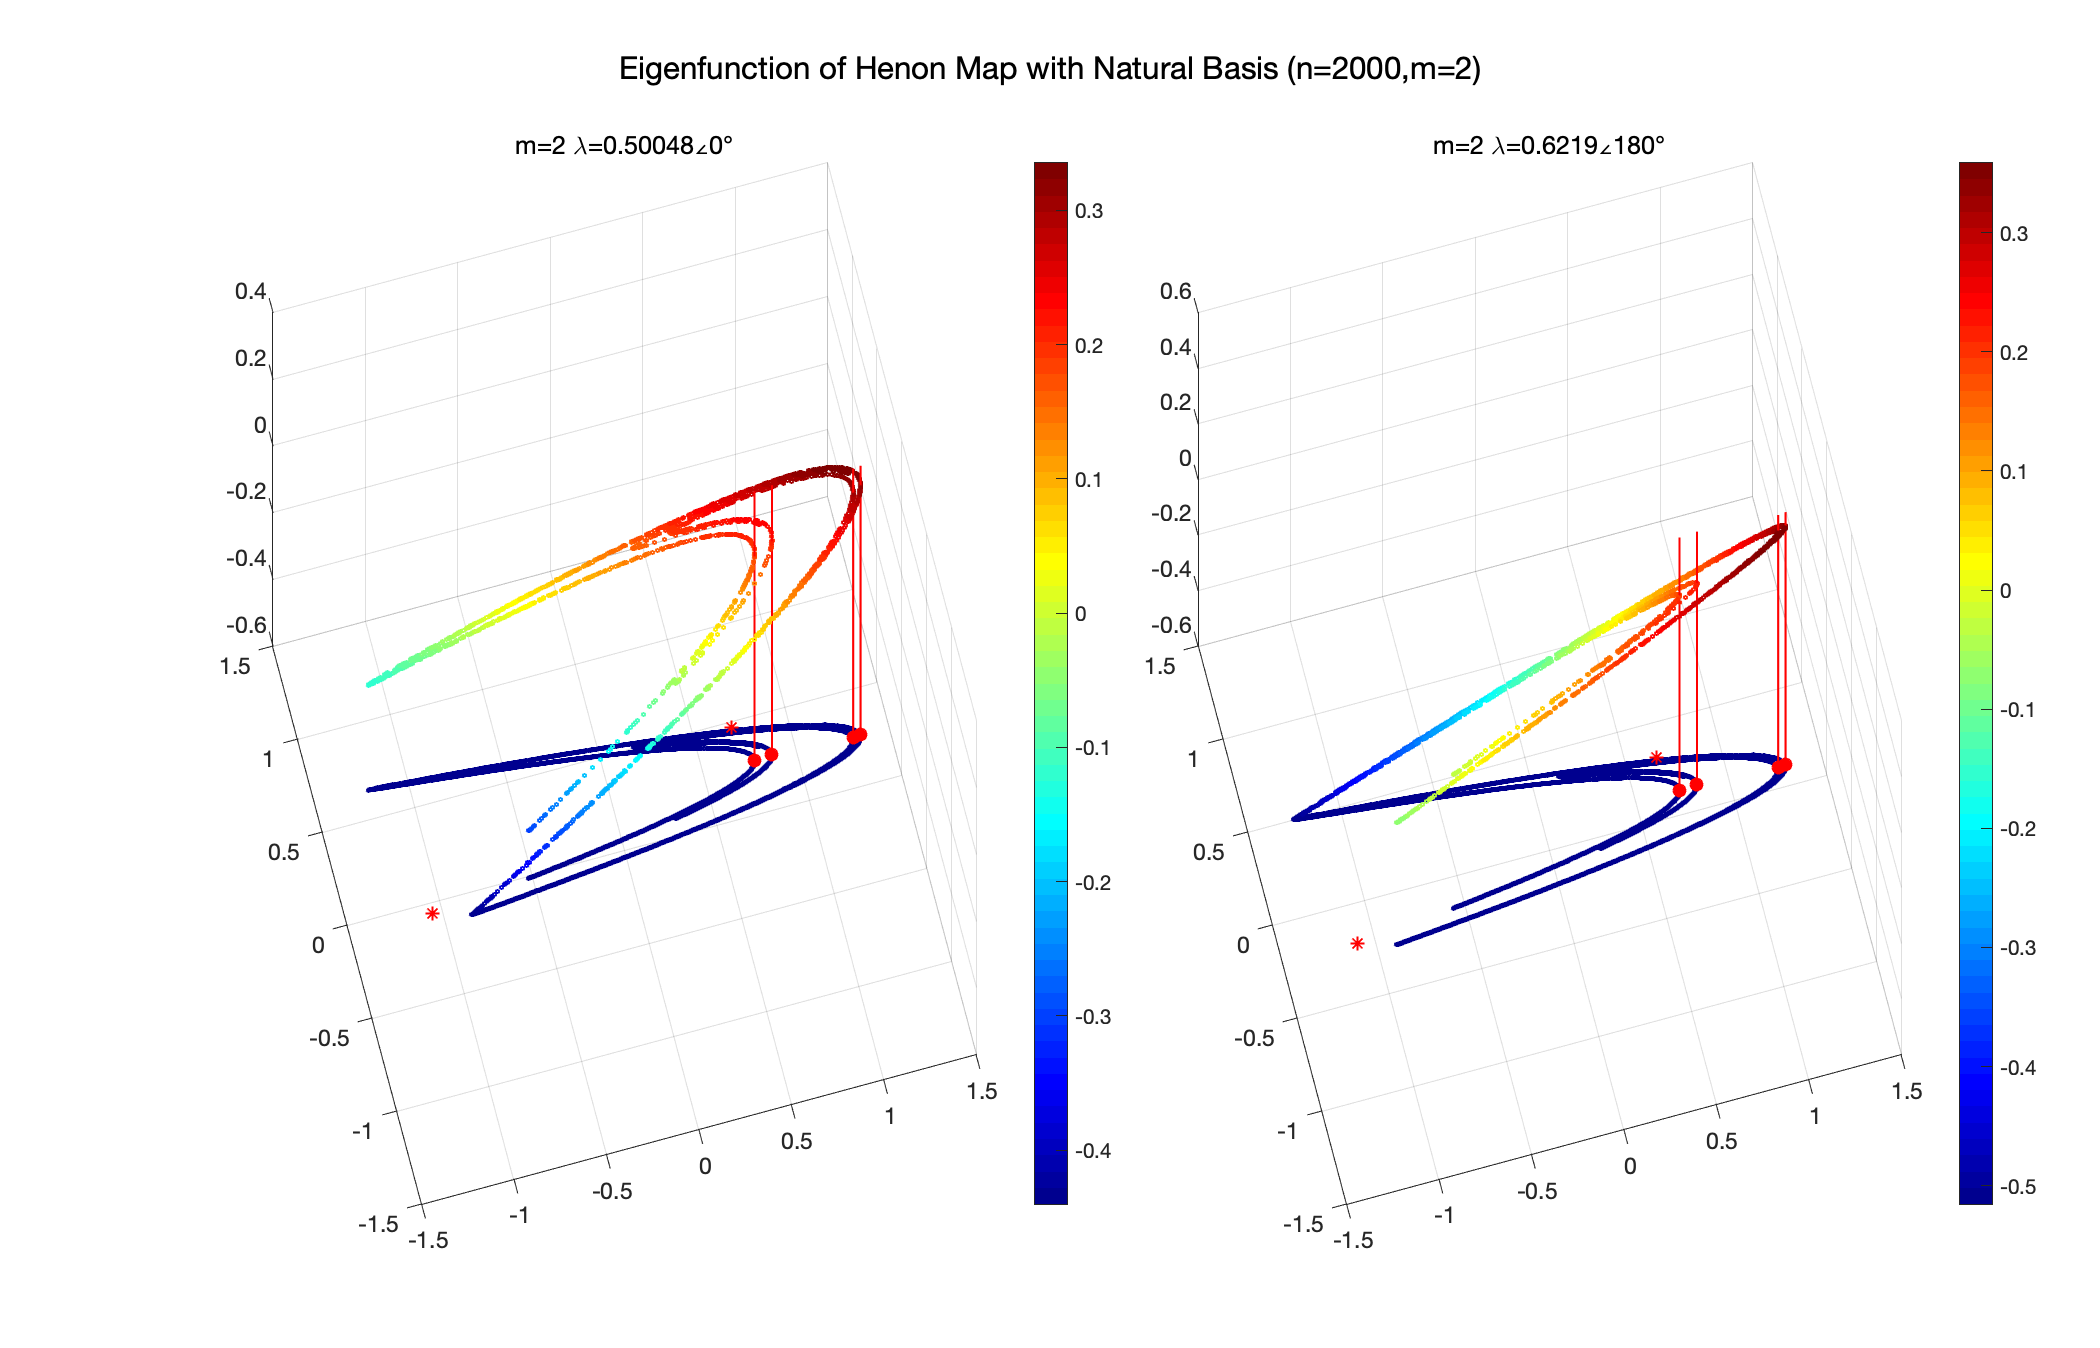
\includegraphics[scale=0.2]{henon/attractors/Henon_eigen_natural_attr_n2000m2}}
    \\
    \subfloat[m=3]{
      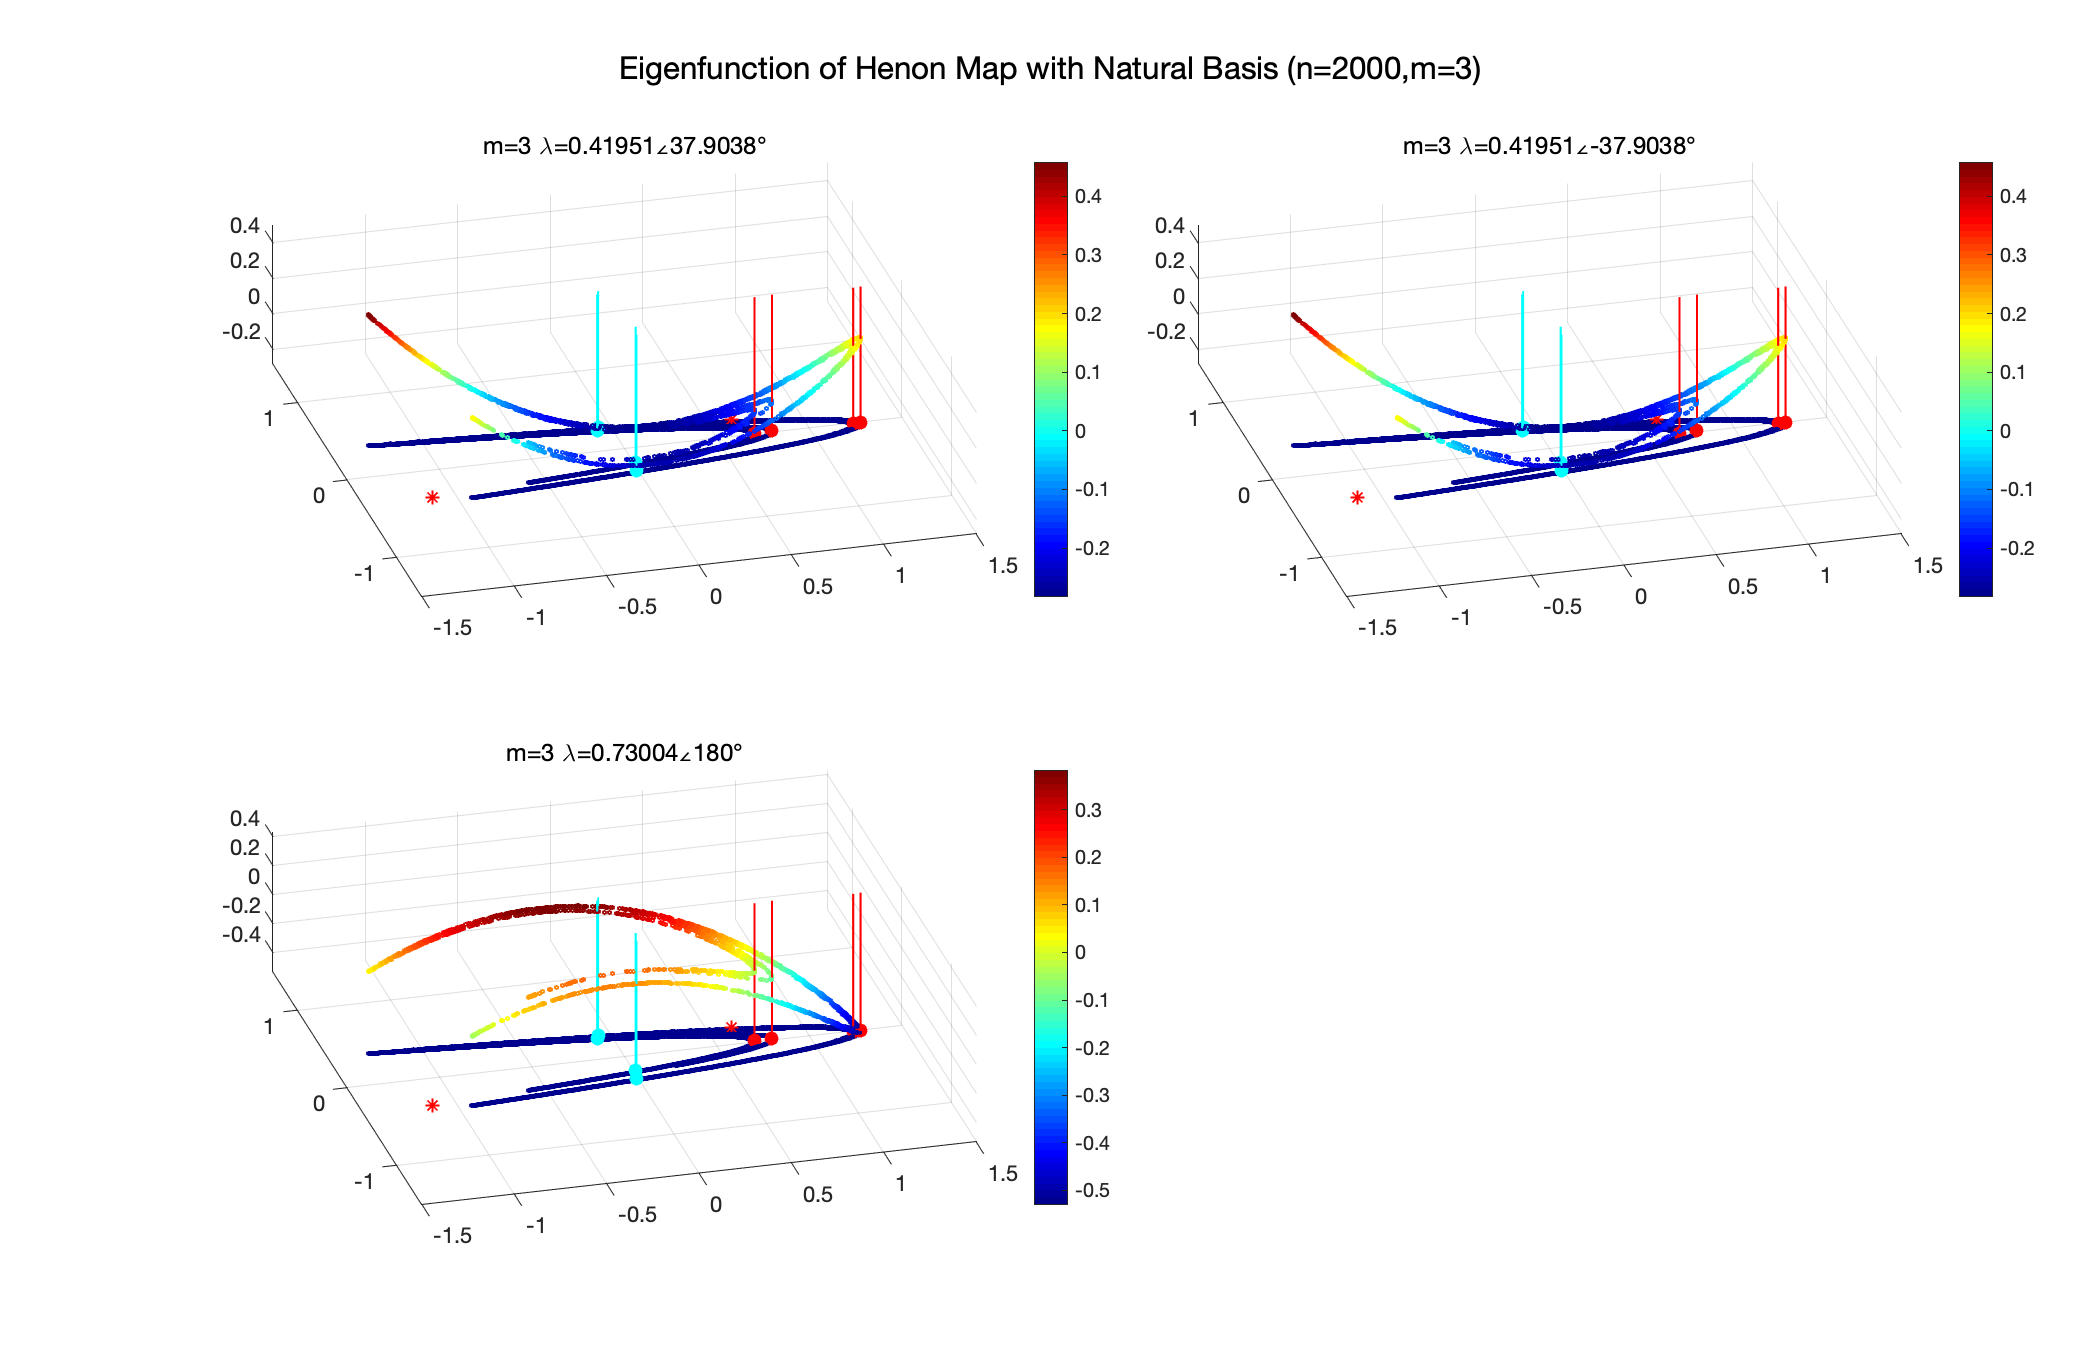
\includegraphics[scale=0.2]{henon/attractors/Henon_eigen_natural_attr_n2000m3}}
    \subfloat[m=4]{
      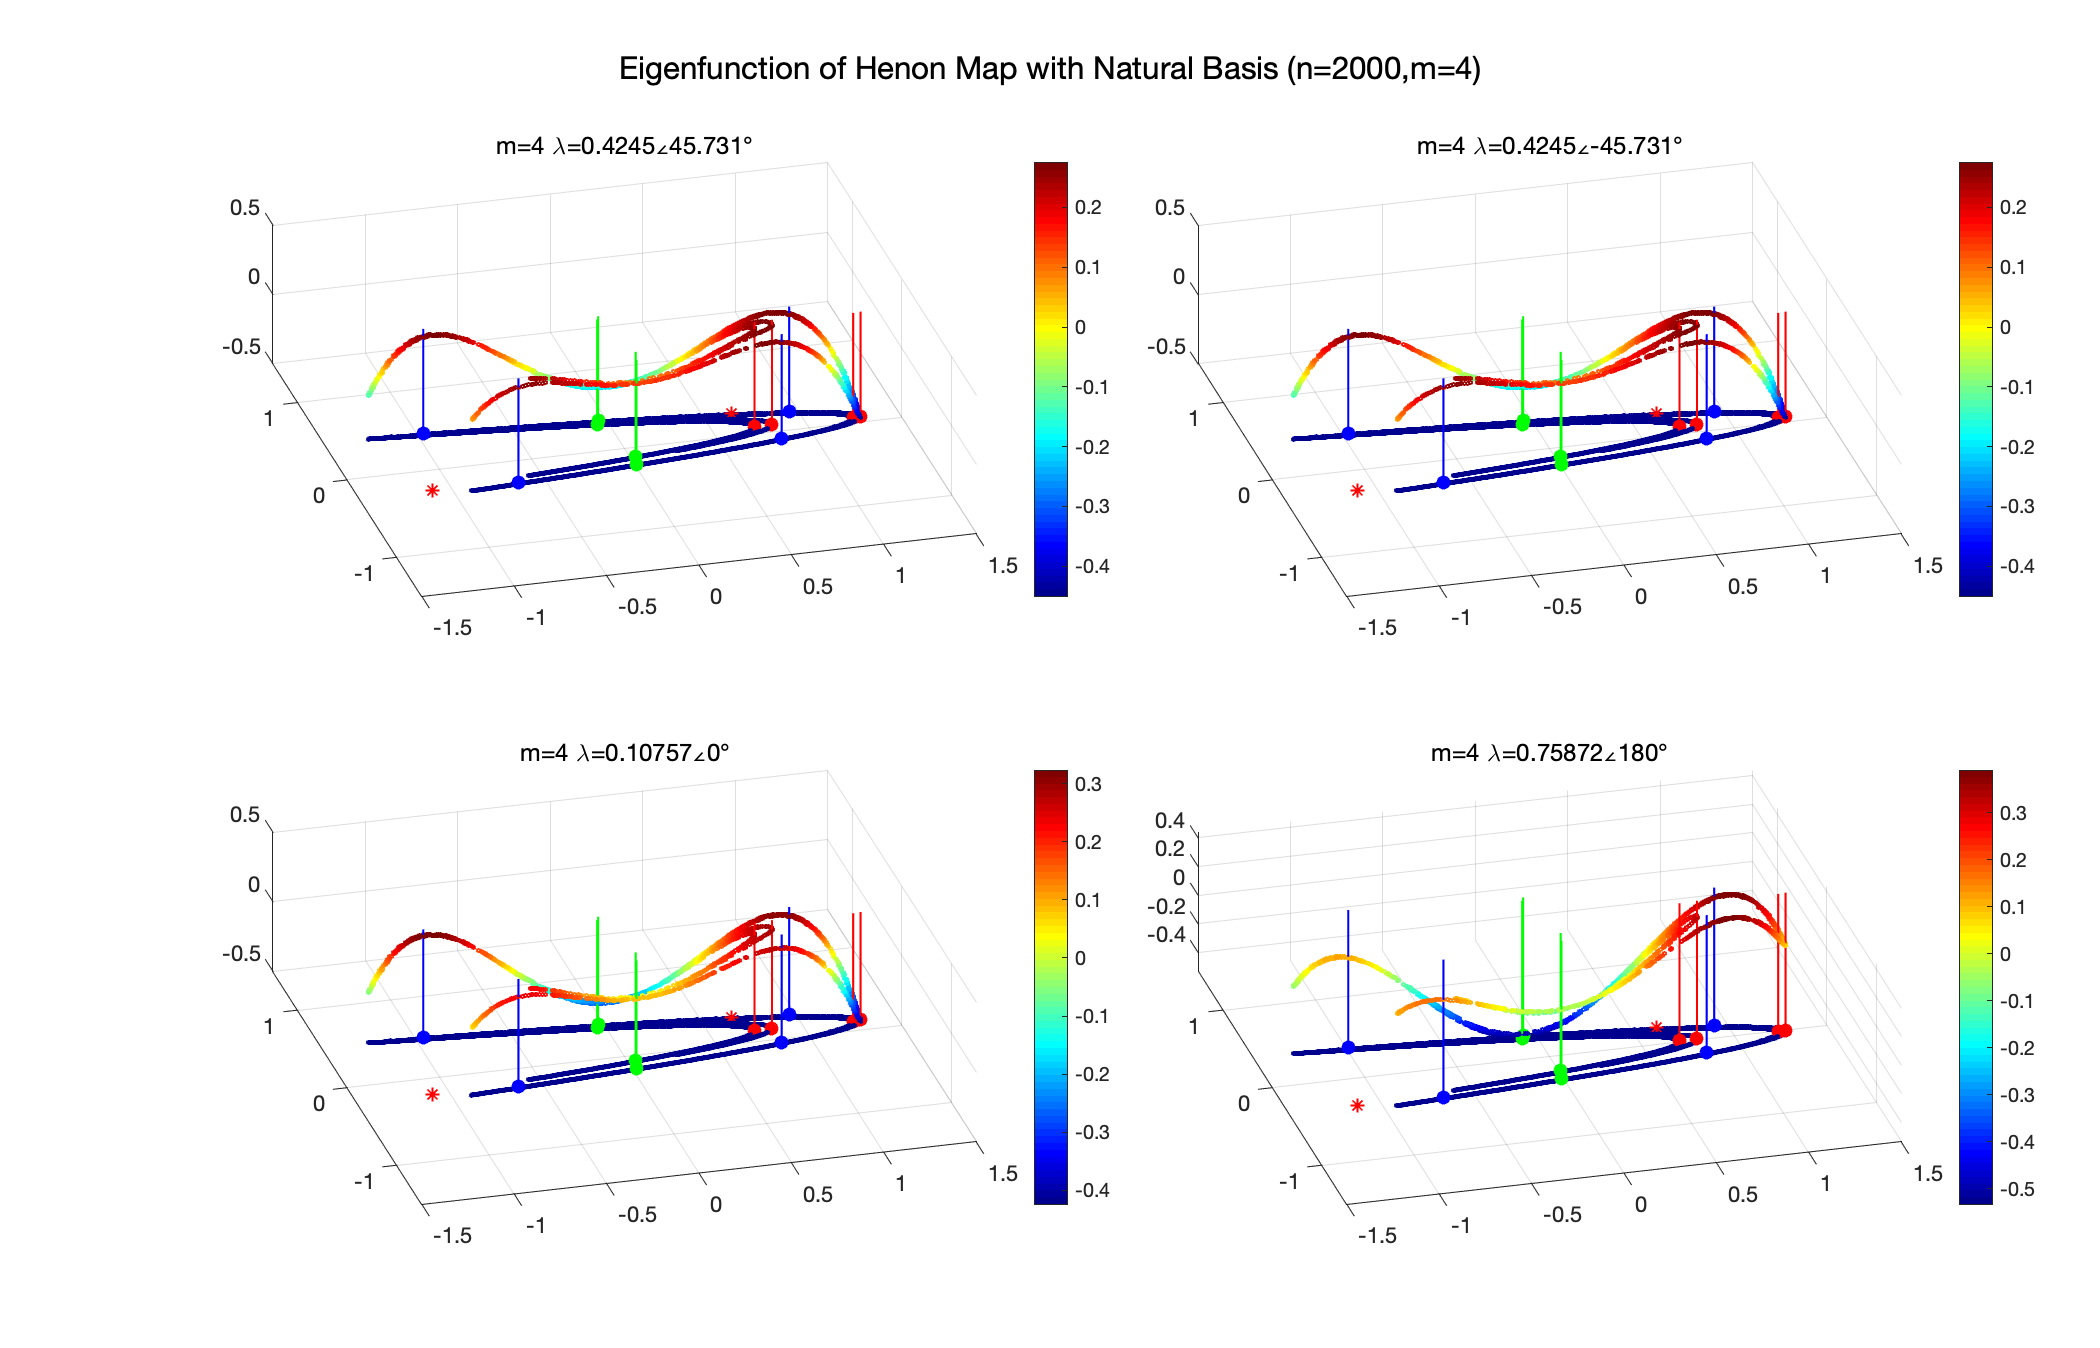
\includegraphics[scale=0.2]{henon/attractors/Henon_eigen_natural_attr_n2000m4}}
    \\
    \subfloat[m=5]{
      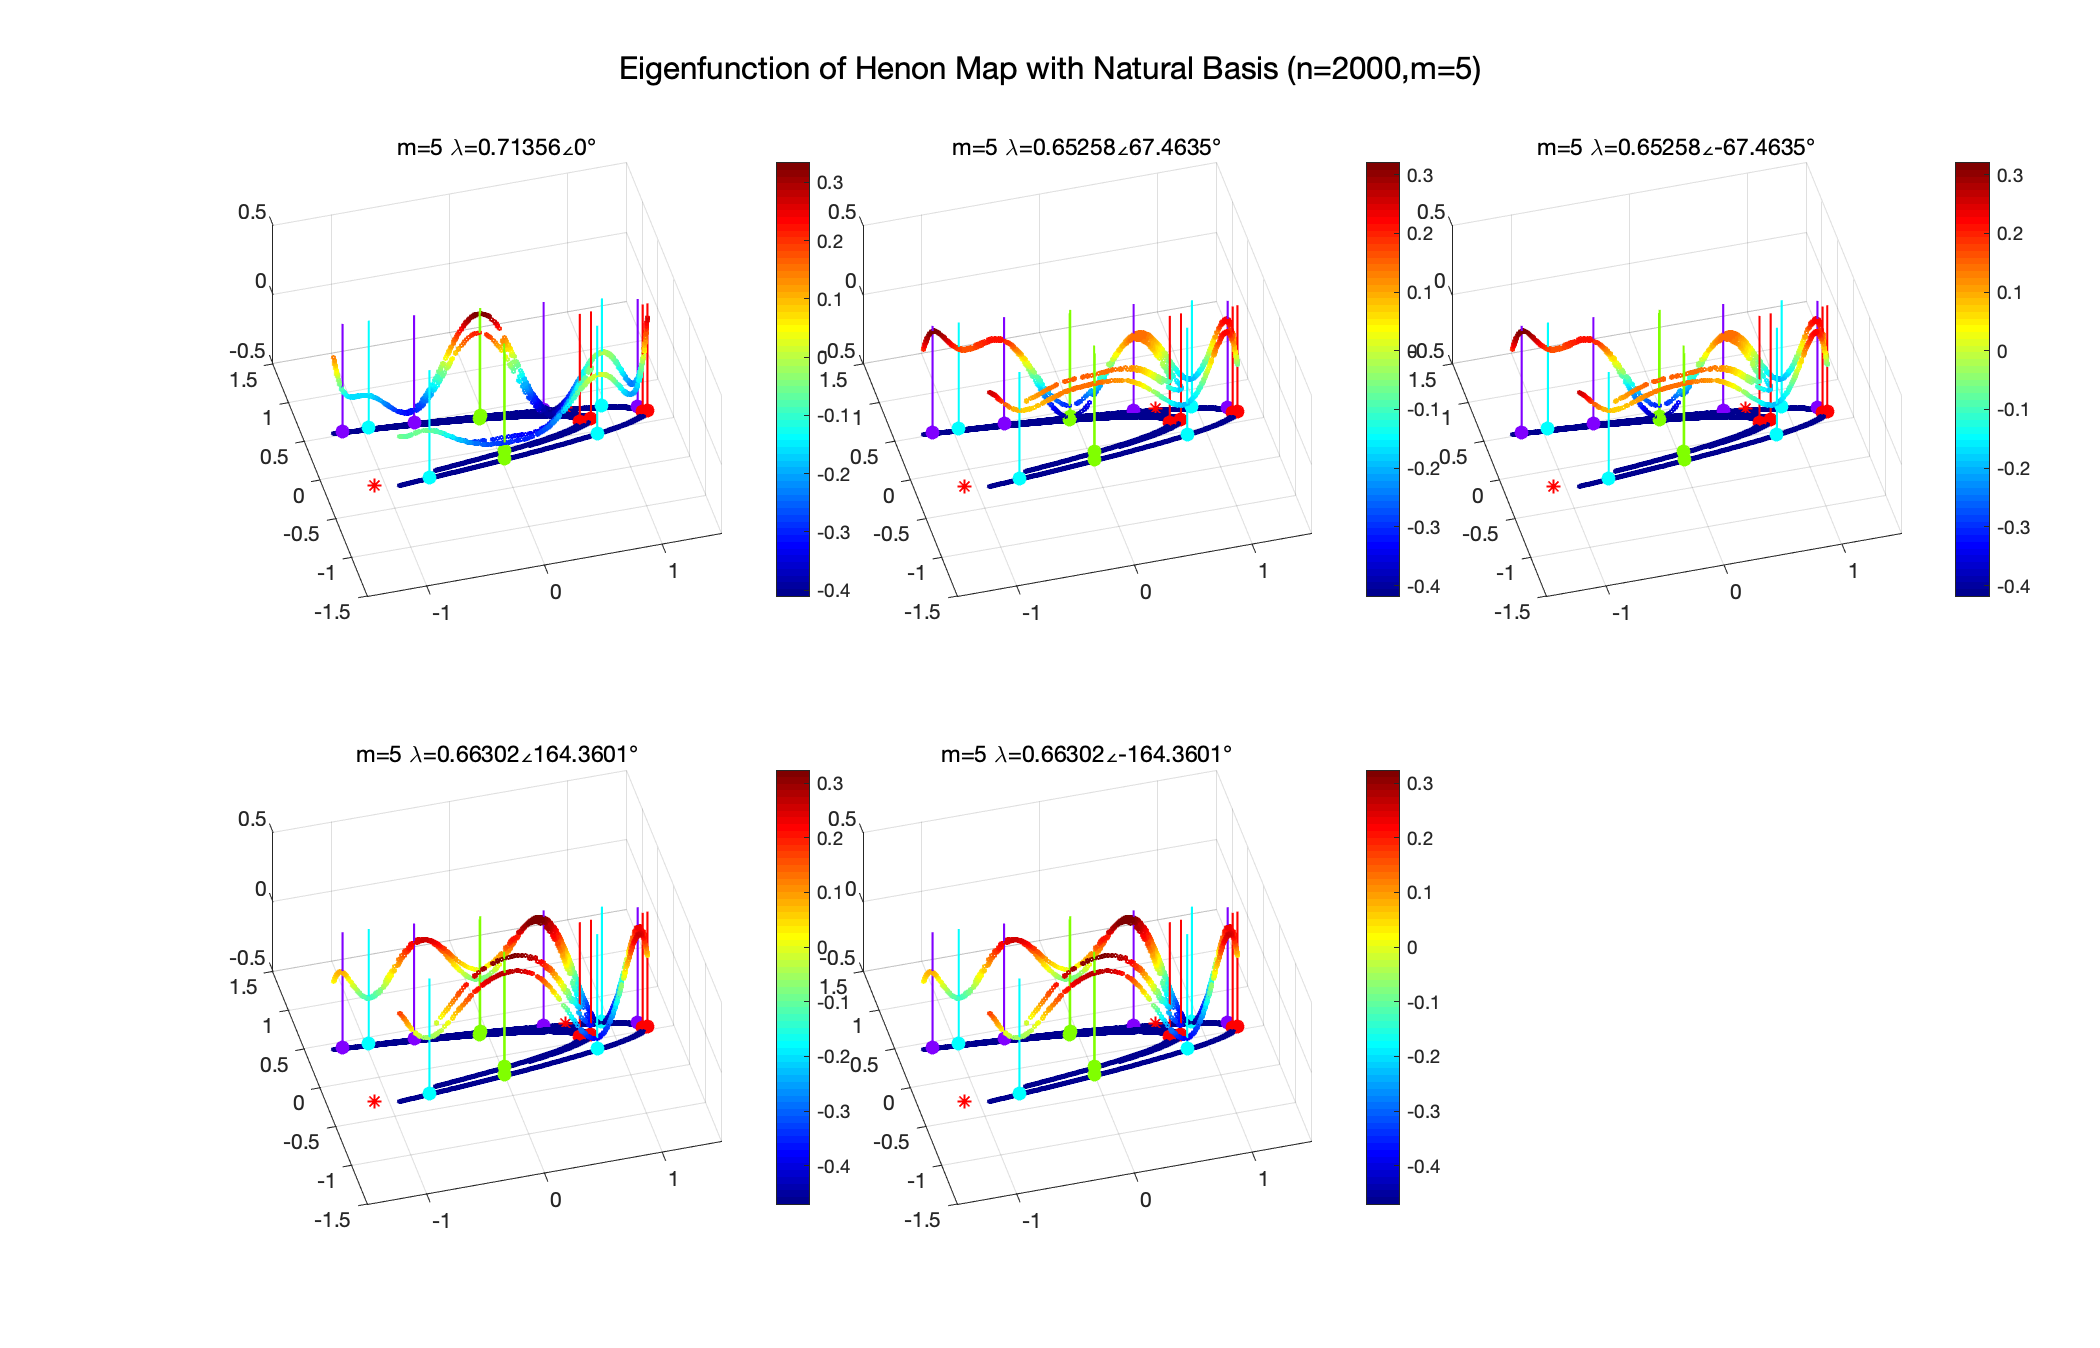
\includegraphics[scale=0.2]{henon/attractors/Henon_eigen_natural_attr_n2000m5}}
    \subfloat[m=6]{
      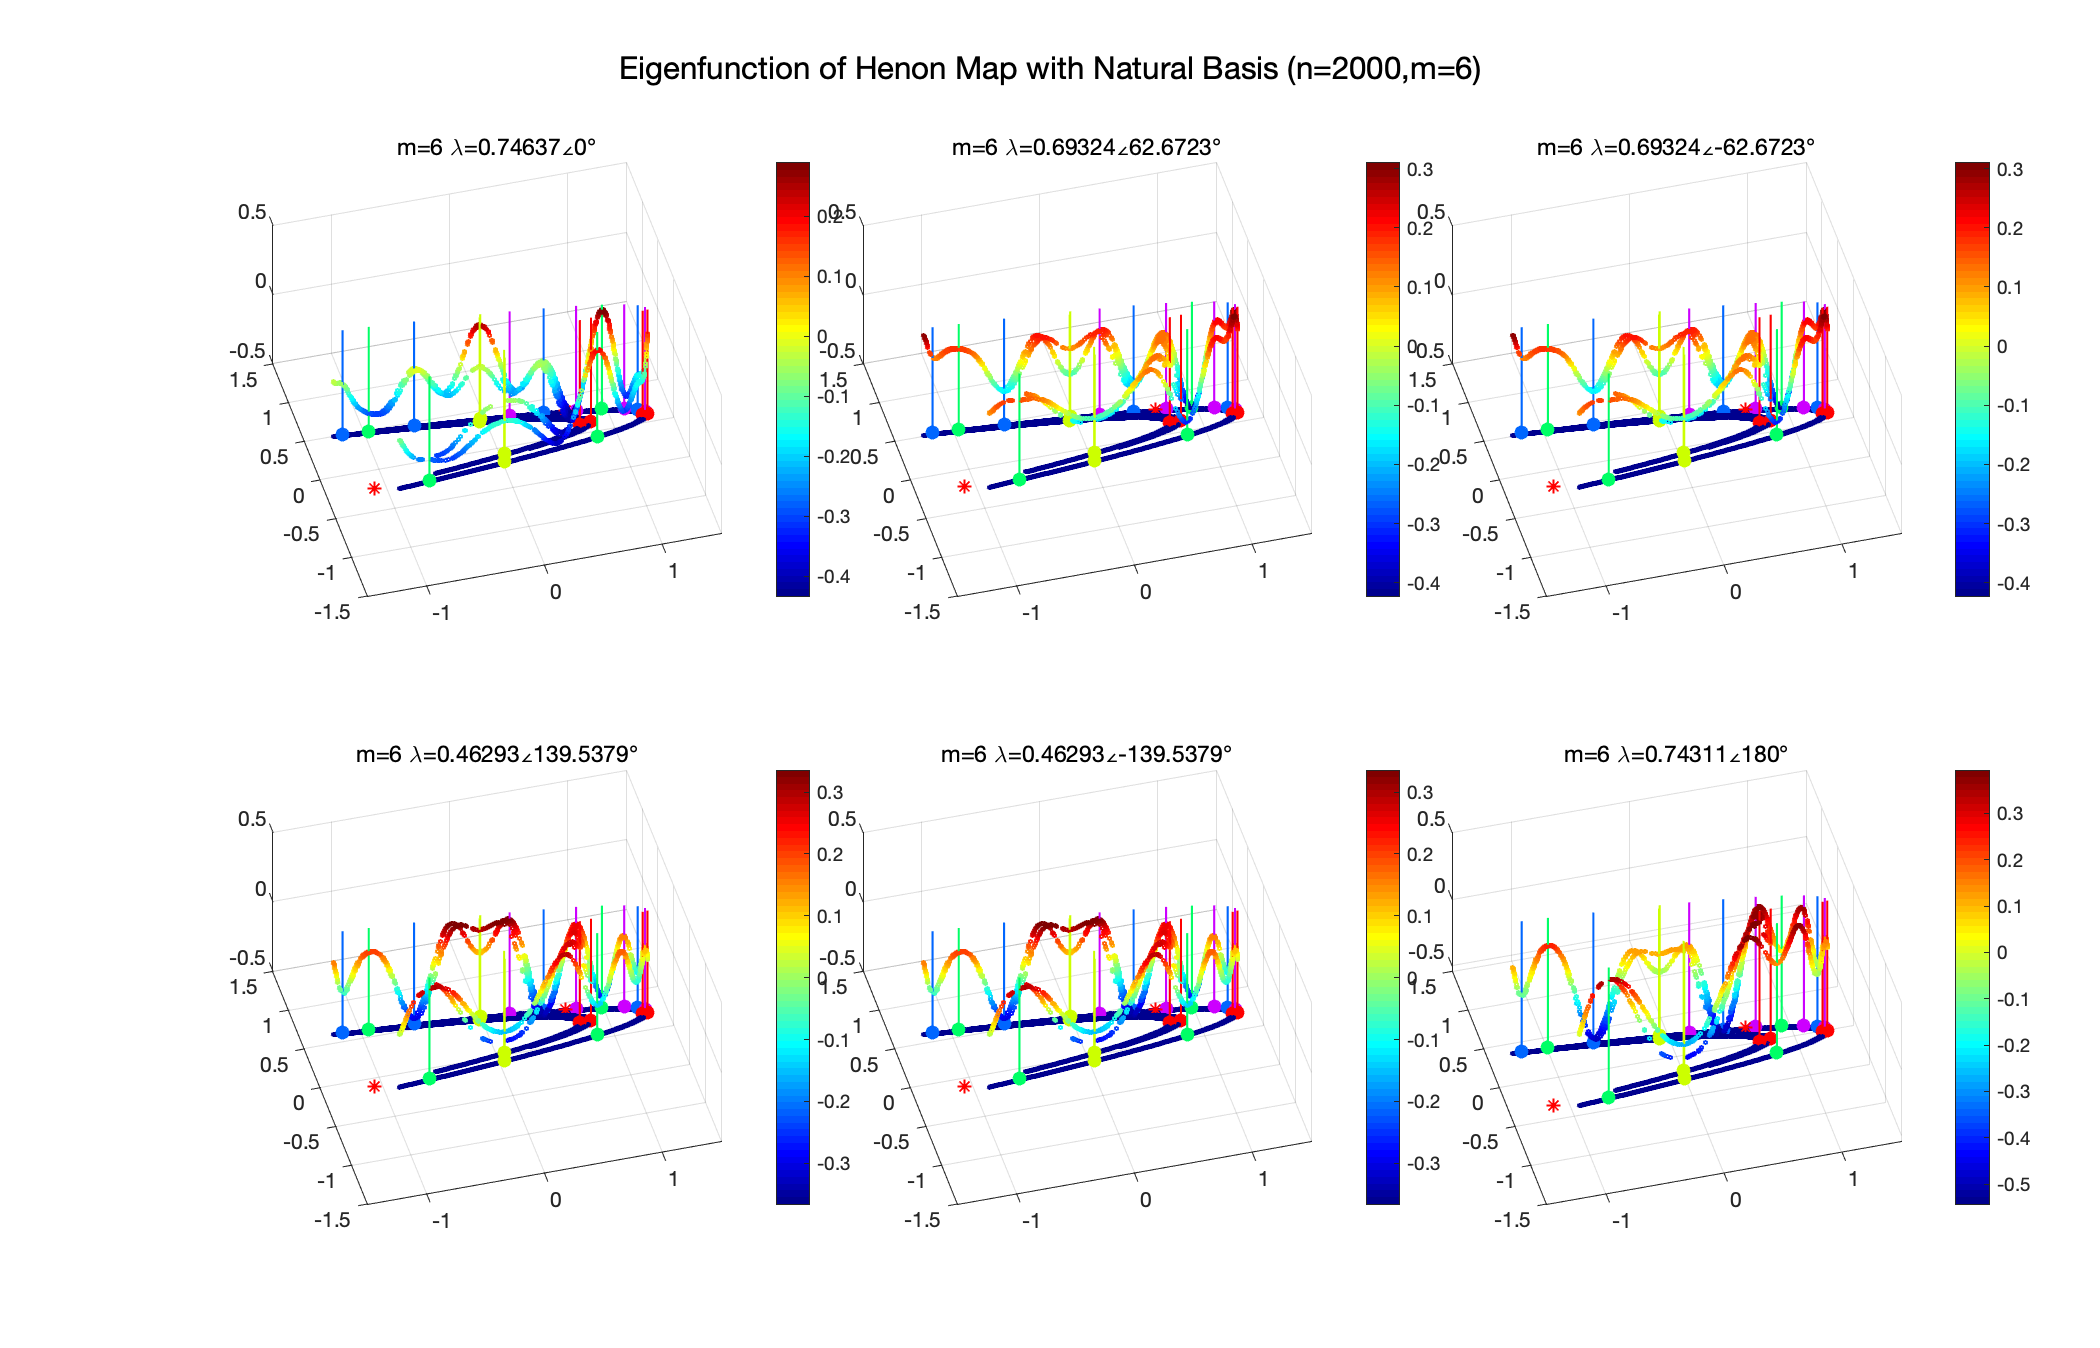
\includegraphics[scale=0.2]{henon/attractors/Henon_eigen_natural_attr_n2000m6}}
    \\
    \subfloat[m=7]{
      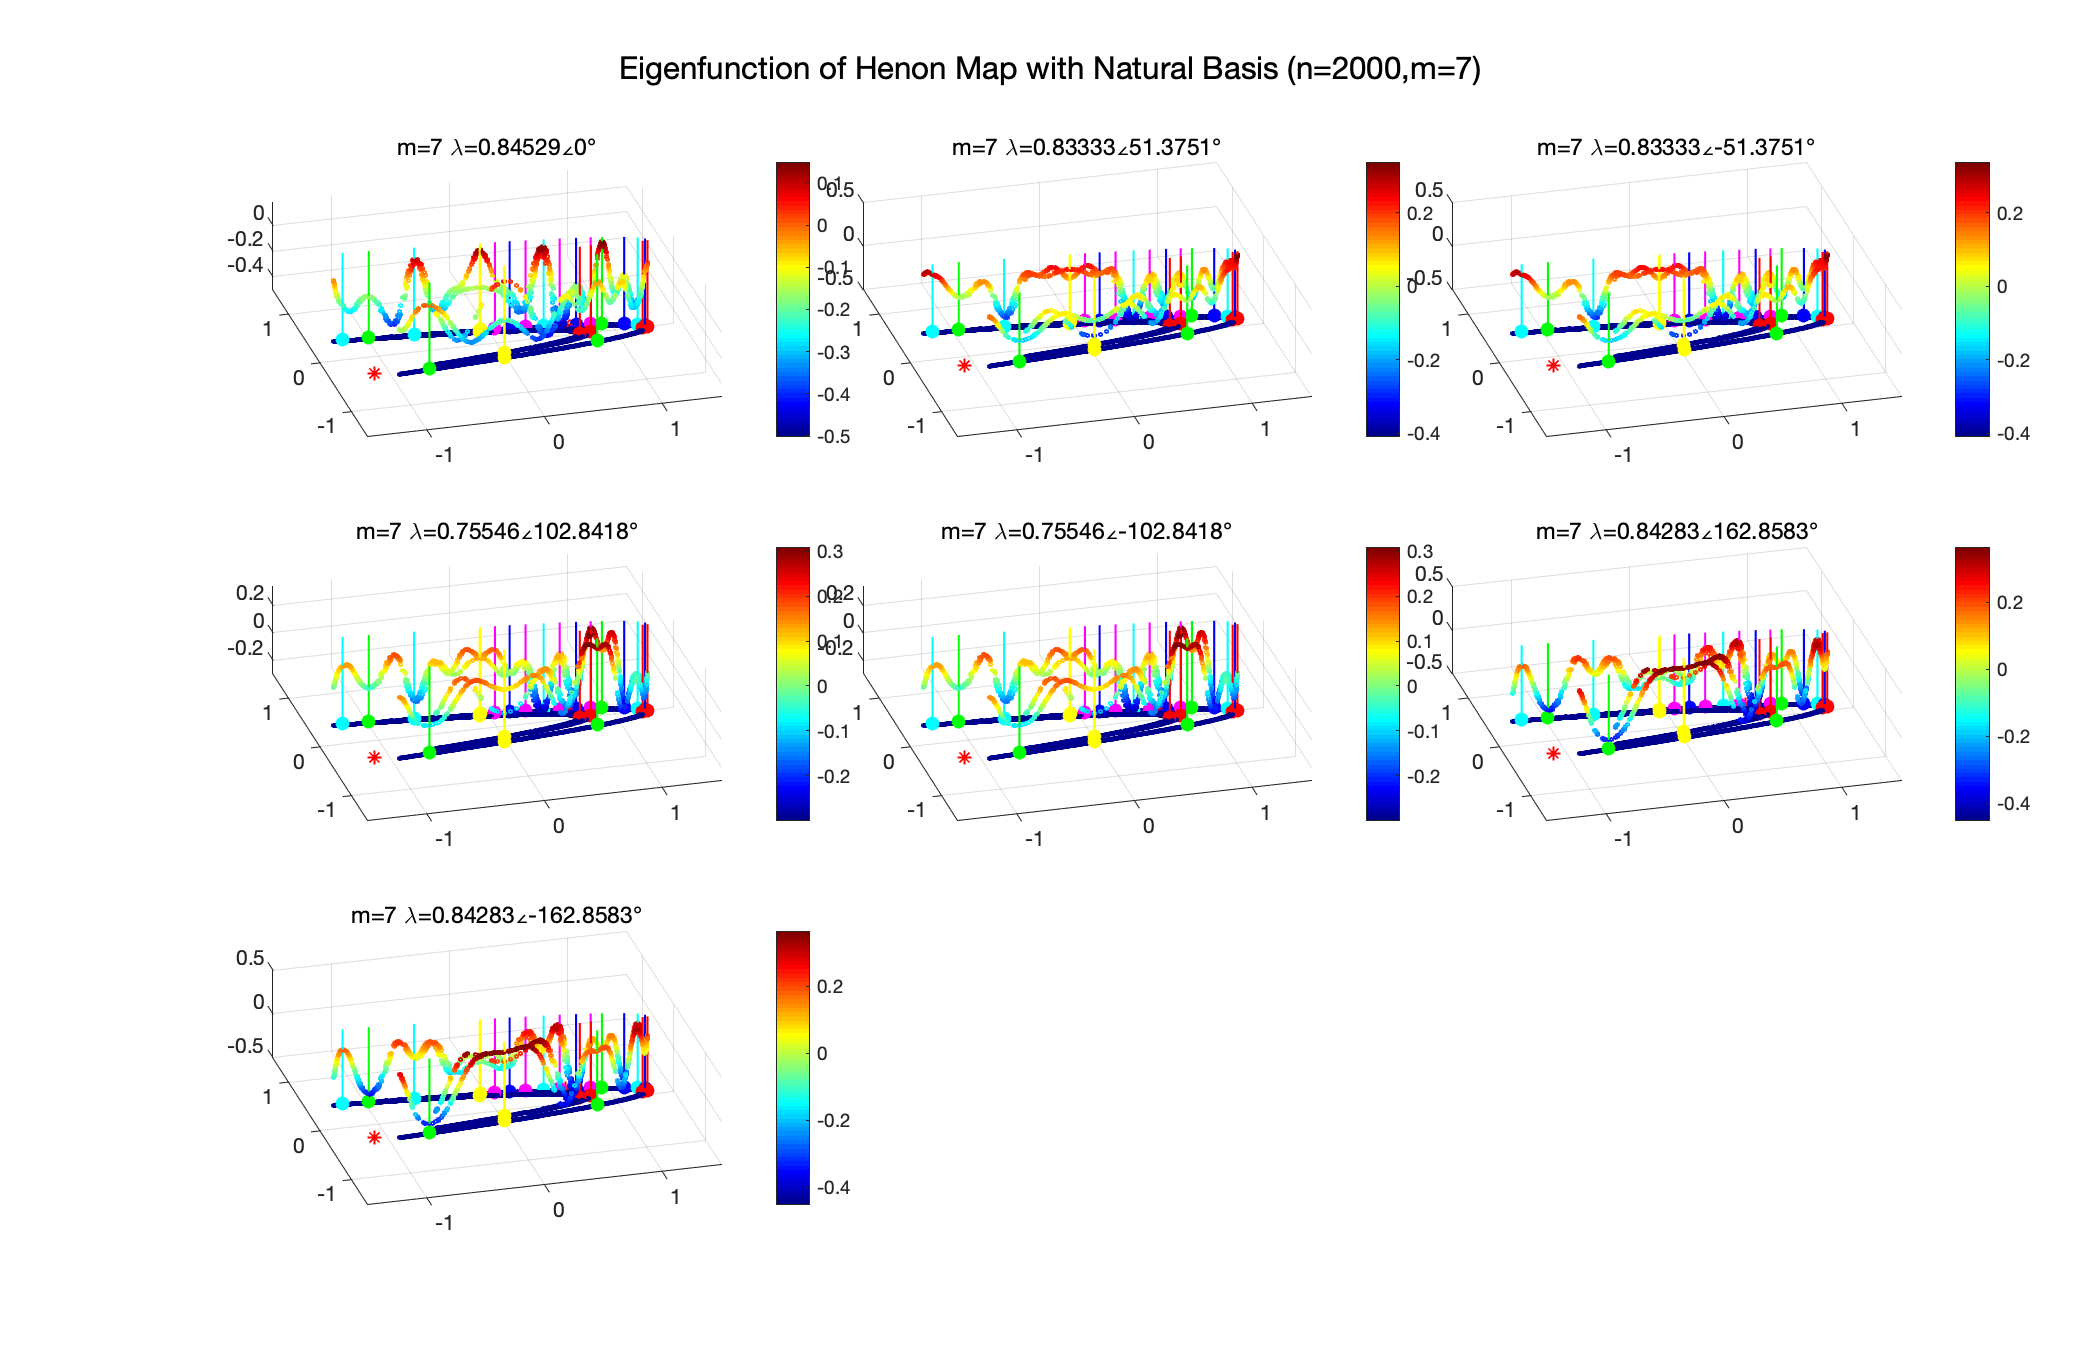
\includegraphics[scale=0.2]{henon/attractors/Henon_eigen_natural_attr_n2000m7}}
    \subfloat[m=8]{
      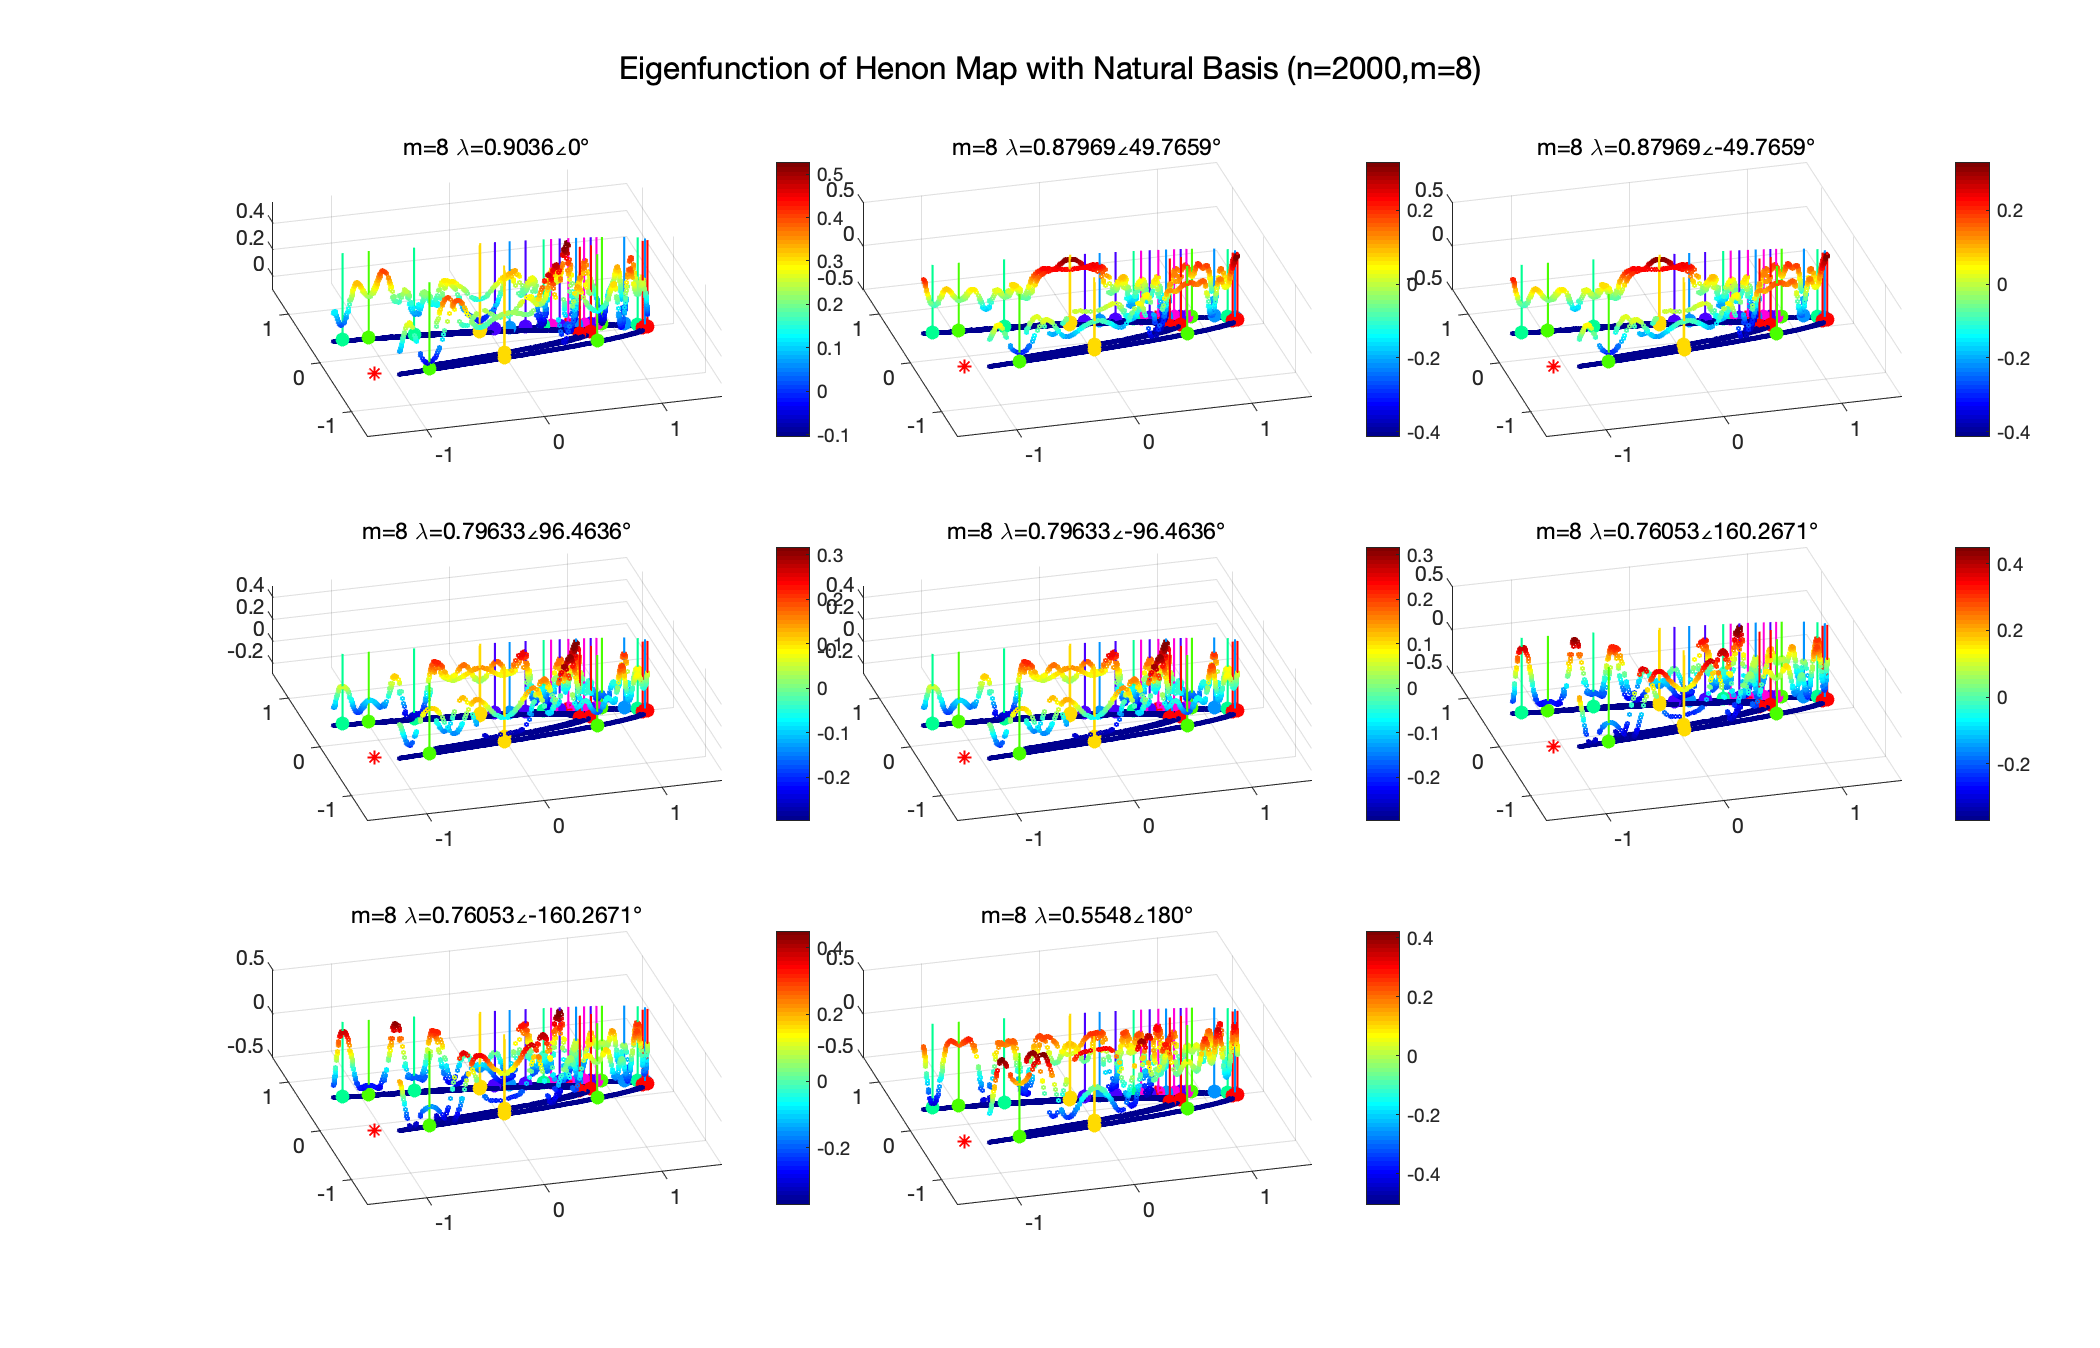
\includegraphics[scale=0.2]{henon/attractors/Henon_eigen_natural_attr_n2000m8}}
    \\
    \caption[埃农映射的边界点与本征函数对吸引子的划分]{埃农映射的边界点与本征函数对吸引子的划分($n=2000$):彩色的点表示本征函数值,蓝色的点表示本征函数在xy平面上的投影,在投影上我们用不同颜色的点标注了不同层次的边界点位置,且将这些点沿z轴正方向延伸便于对比}\label{fig:Henon_eigen_natural_attr_n2000m8}
\end{figure}
在图\ref{fig:Henon_eigen_natural_attr_n2000m8}(b)中,基函数数量$m=2$,本征函数在每条线上存在1个极值点共计4个极值点且与我们层次为0的边界点一一对应,在图\ref{fig:Henon_eigen_natural_attr_n2000m8}(c)中,基函数数量$m=3$,本征函数在每条线上存在三个极值点,且与我们层次为$-1,0$的边界点一一对应,同样的,随着基函数数量的增多,本征函数图像的极值点也随之增多,我们也将更多层次的边界点画在图中,我们发现,本征函数值的极值点总是能和埃农映射的边界点有着对应关系,并且基函数数量每增加1,本征函数图像反映的边界点层次也随之增加1。这个结论与一维映射的结论一致,且定量的描述了基函数数量的增加对边界点层次的影响。

\begin{figure}
	\centering
	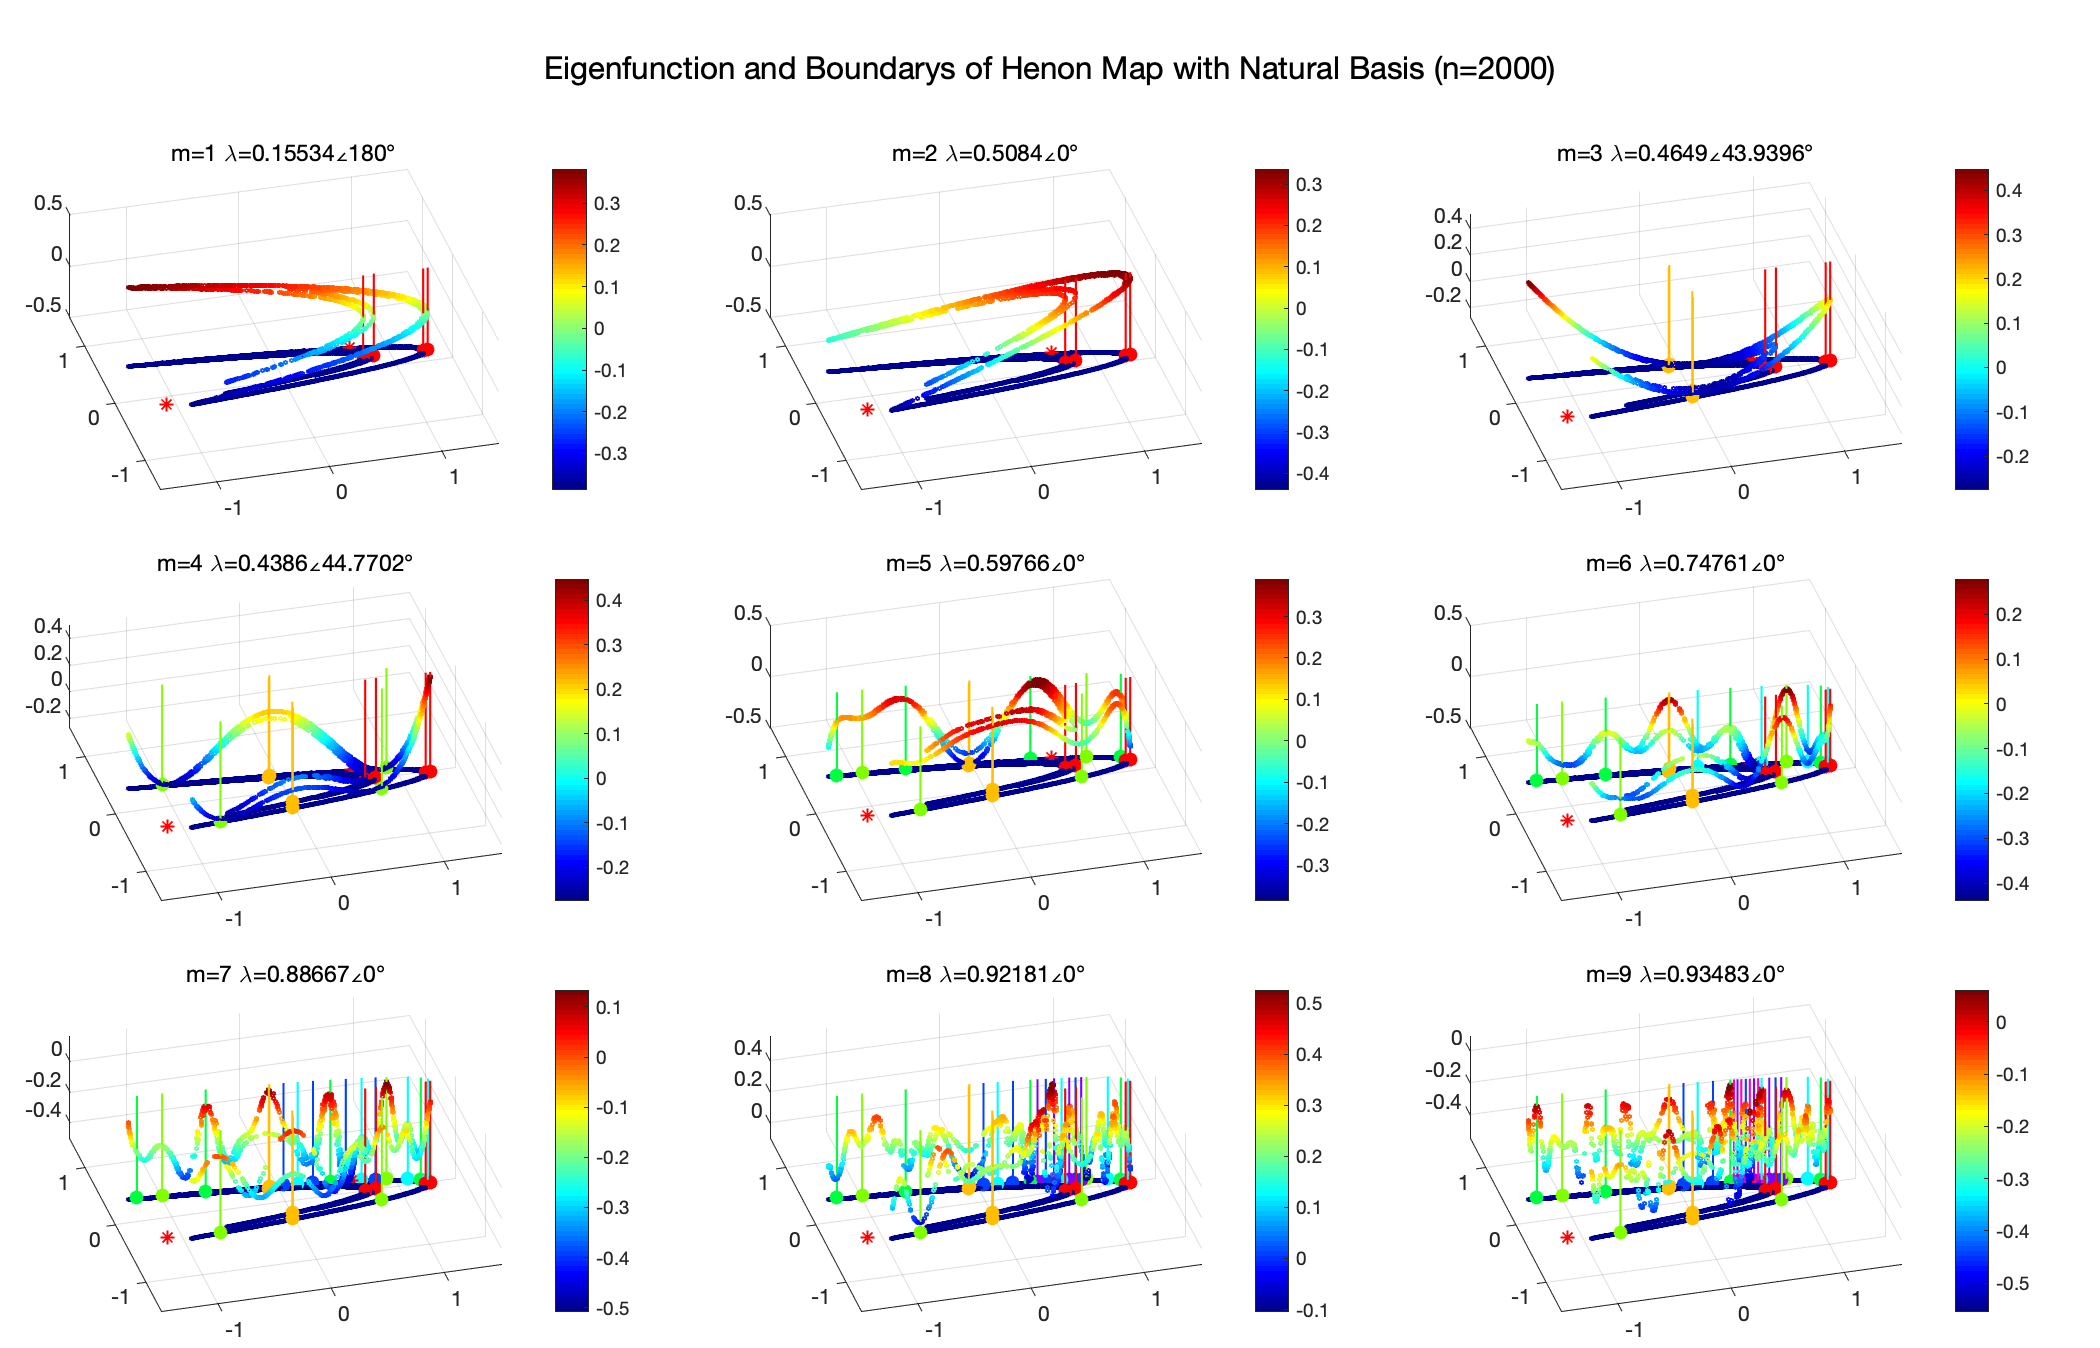
\includegraphics[scale=0.4]{henon/attractors/Henon_eigen_natural_attr_n2000}
    \caption{埃农映射的边界点与本征函数对吸引子的划分($n=2000$)}\label{fig:Henon_eigen_natural_attr_n2000}
\end{figure}

为了反映这种变化关系,我们每个基函数数量下取一个本征函数,画出随基函数增加,本征函数极值点与埃农映射边界点的关系,如图\ref{fig:Henon_eigen_natural_attr_n2000}。从图中,我们可以更清晰的发现这个结论:Koopman算符的本征值反映了埃农映射的边界点,且随着基函数数量的增加,能够反映出埃农映射不同层次的边界点,基函数数量每增加1,埃农映射的边界点便能反映更多一个层次。

\subsection{更多的讨论}
\subsubsection{埃农映射的周期轨道}
在这里我们讨论埃农映射的周期轨道,在第二章中我们讨论了周期轨道对相空间动力学特征的划分,周期轨道也是动力学特征的重要部分。关于埃农映射的周期轨道已有广泛的结论\cite{biham1989characterization}。这里我们通过Multipoint Shooting的方法\cite{yang2009locating}计算得到埃农映射不同周期的周期轨道,如图\ref{fig:Henon_periodic_orbits},我们计算了$T=2,3,4,5,6,8,9,10$时埃农映射的周期轨道。
\begin{figure}
	\centering
	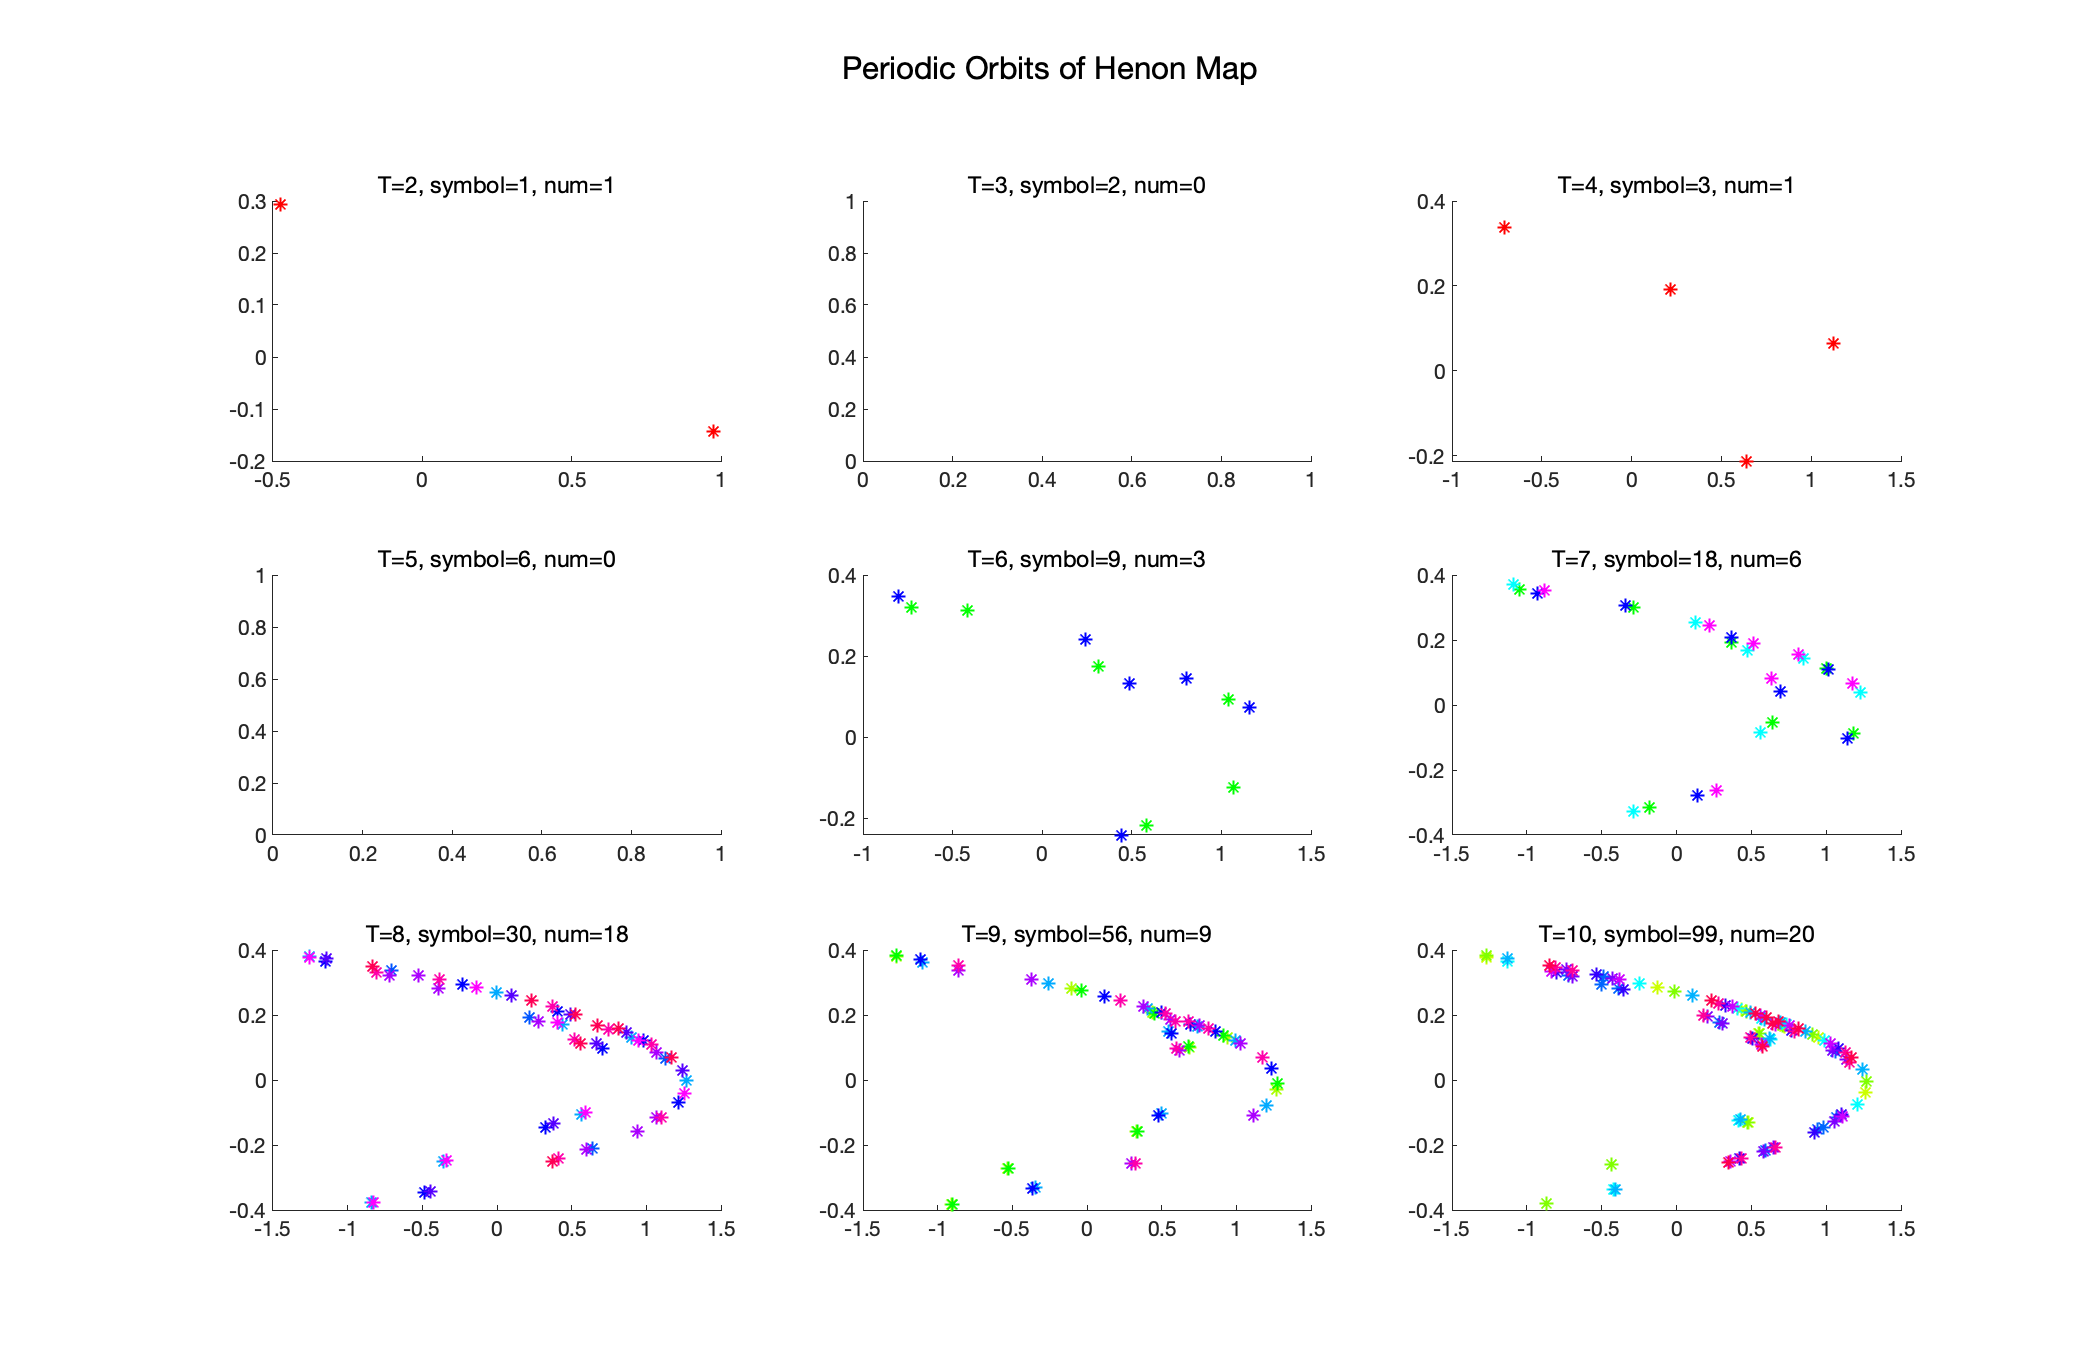
\includegraphics[scale=0.4]{henon/period/Henon_periodic_orbits}
    \caption[埃农映射的周期轨道]{埃农映射的周期轨道:在每个子图的标题中,T表示周期,symbol表示符号动力学允许的最多轨道数,num表示我们寻找到的收敛的轨道数量,并将这些轨道画在同一张图中,num=0表示没有计算到该周期下的轨道,但并不意味着不存在此周期,因为Multipoint Shooting的方法受到初始点选取的限制}\label{fig:Henon_periodic_orbits}
\end{figure}
在第二章的讨论中我们了解到,在离散映射系统中,设有一周期为$T$的动力学系统$x_{n+T}=f^T(x_n)=x_n$,若定义一个新的映射$F=f^T$,则对于新的映射$F$,我们有$F(x_n)=x_n$,即$x_n$为新映射系统的不动点。新映射$F$与原映射$f$之间为$T$次映射,在相空间可表示为$T$次重复变换过程。为此,我们将周期点看作新映射的不动点,并将这些不动点在新映射上进行线性化,如图\ref{fig:Henon_eigen_Gauss_period_n100m50T7},我们选取本征函数参数:演化格点数量$n=100\times 100$,高斯基函数数量$m=50\times 50$,周期轨道参数$T=2,4,6,7$,分别对比其周期轨道位置及其线性化方向。
\begin{figure}
    \centering
    \subfloat[T=2]{
      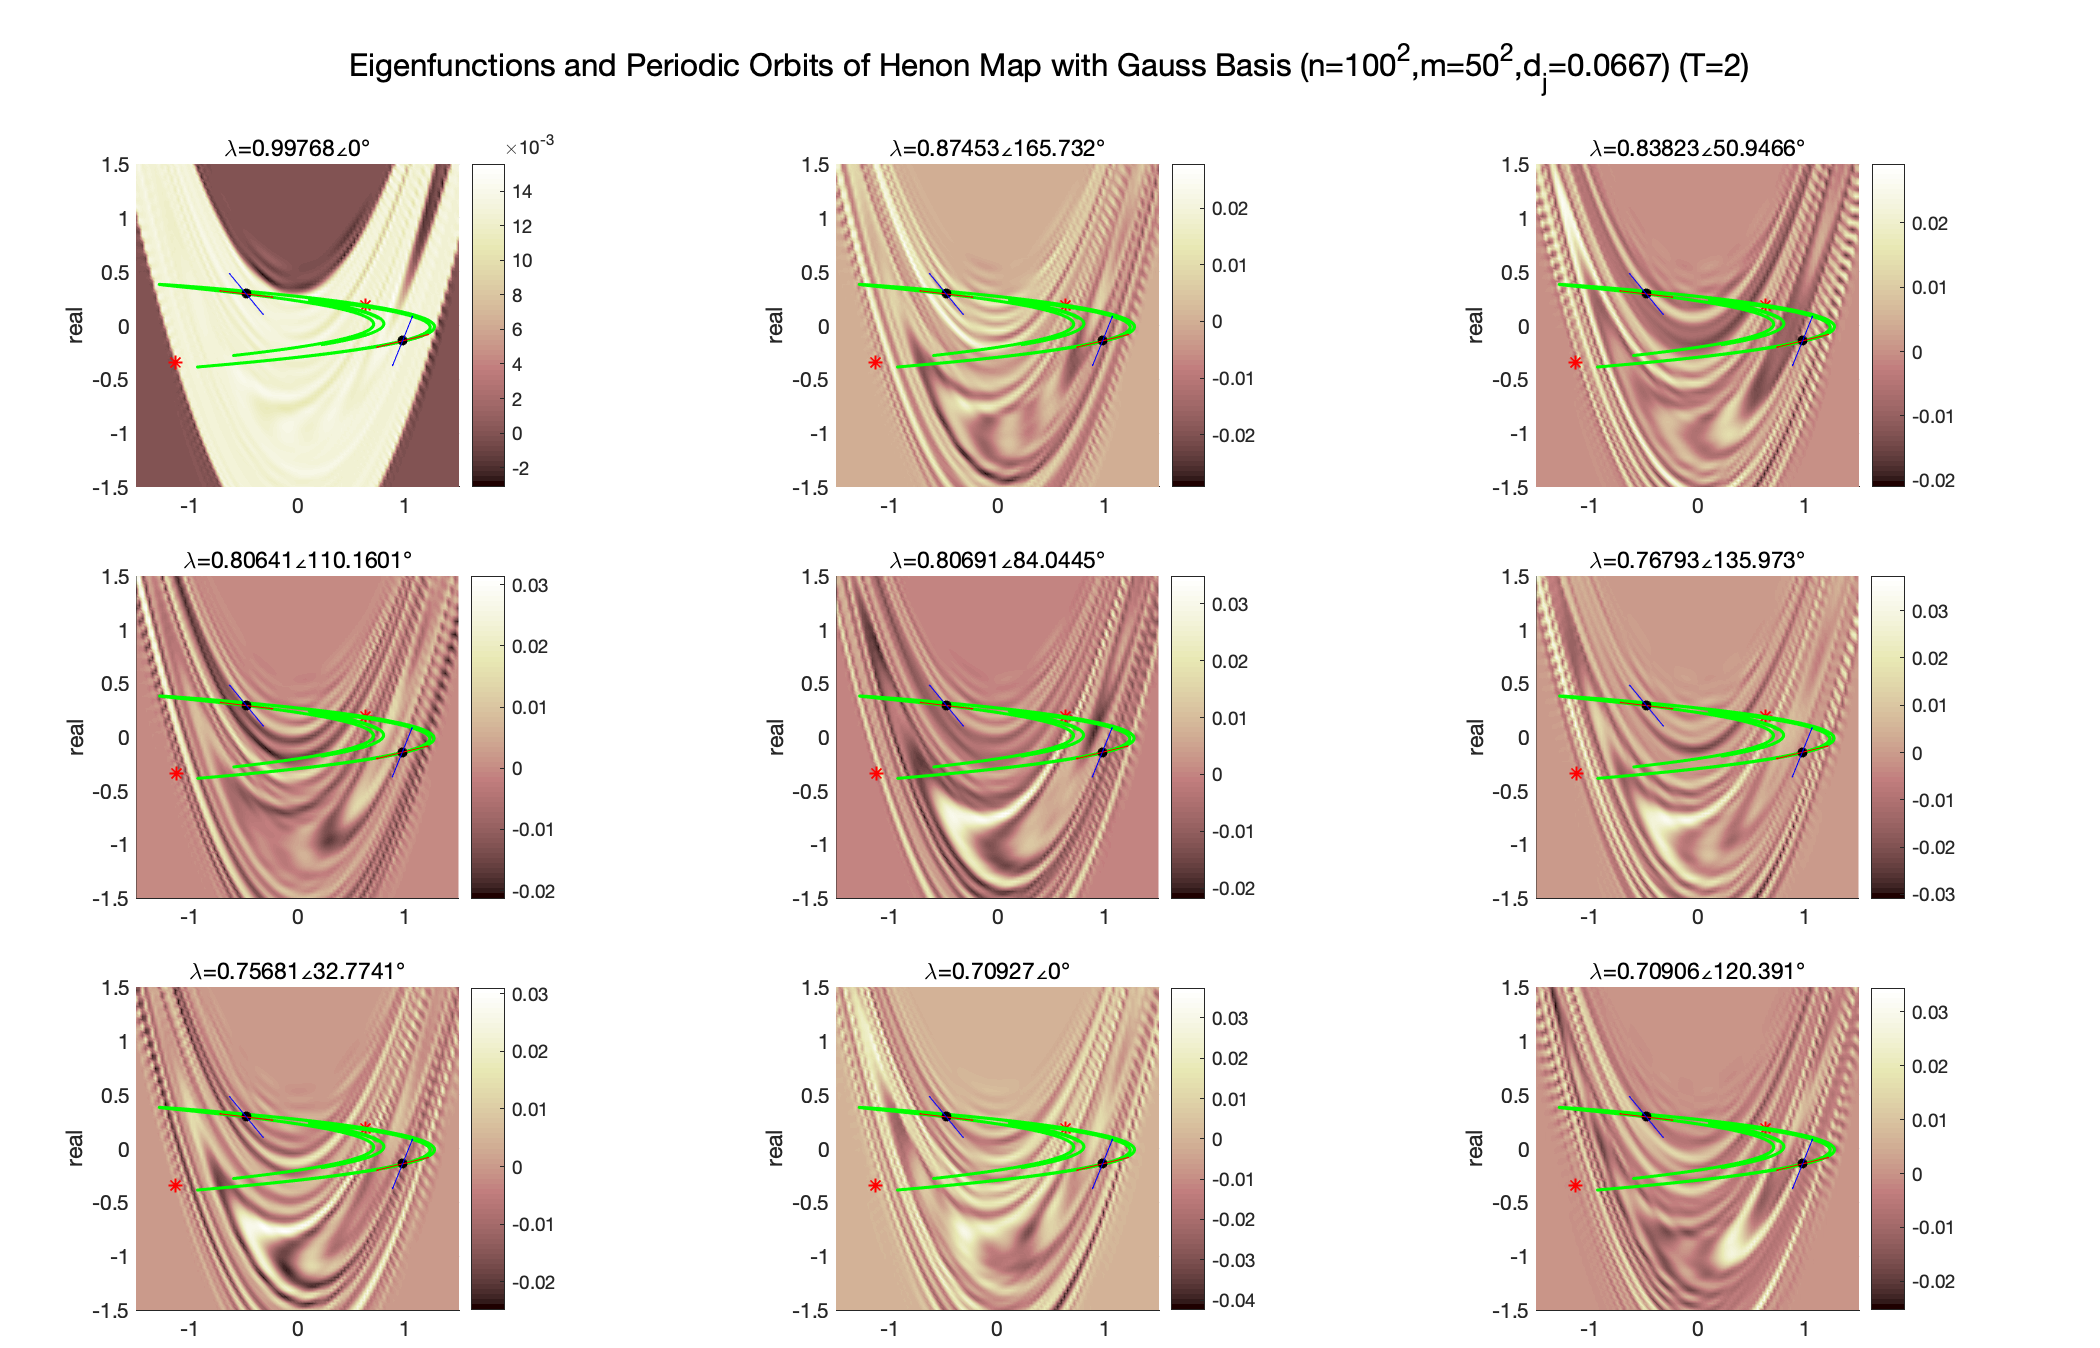
\includegraphics[scale=0.2]{henon/period/Henon_eigen_Gauss_period_n100m50T2}}
    \subfloat[T=4]{
      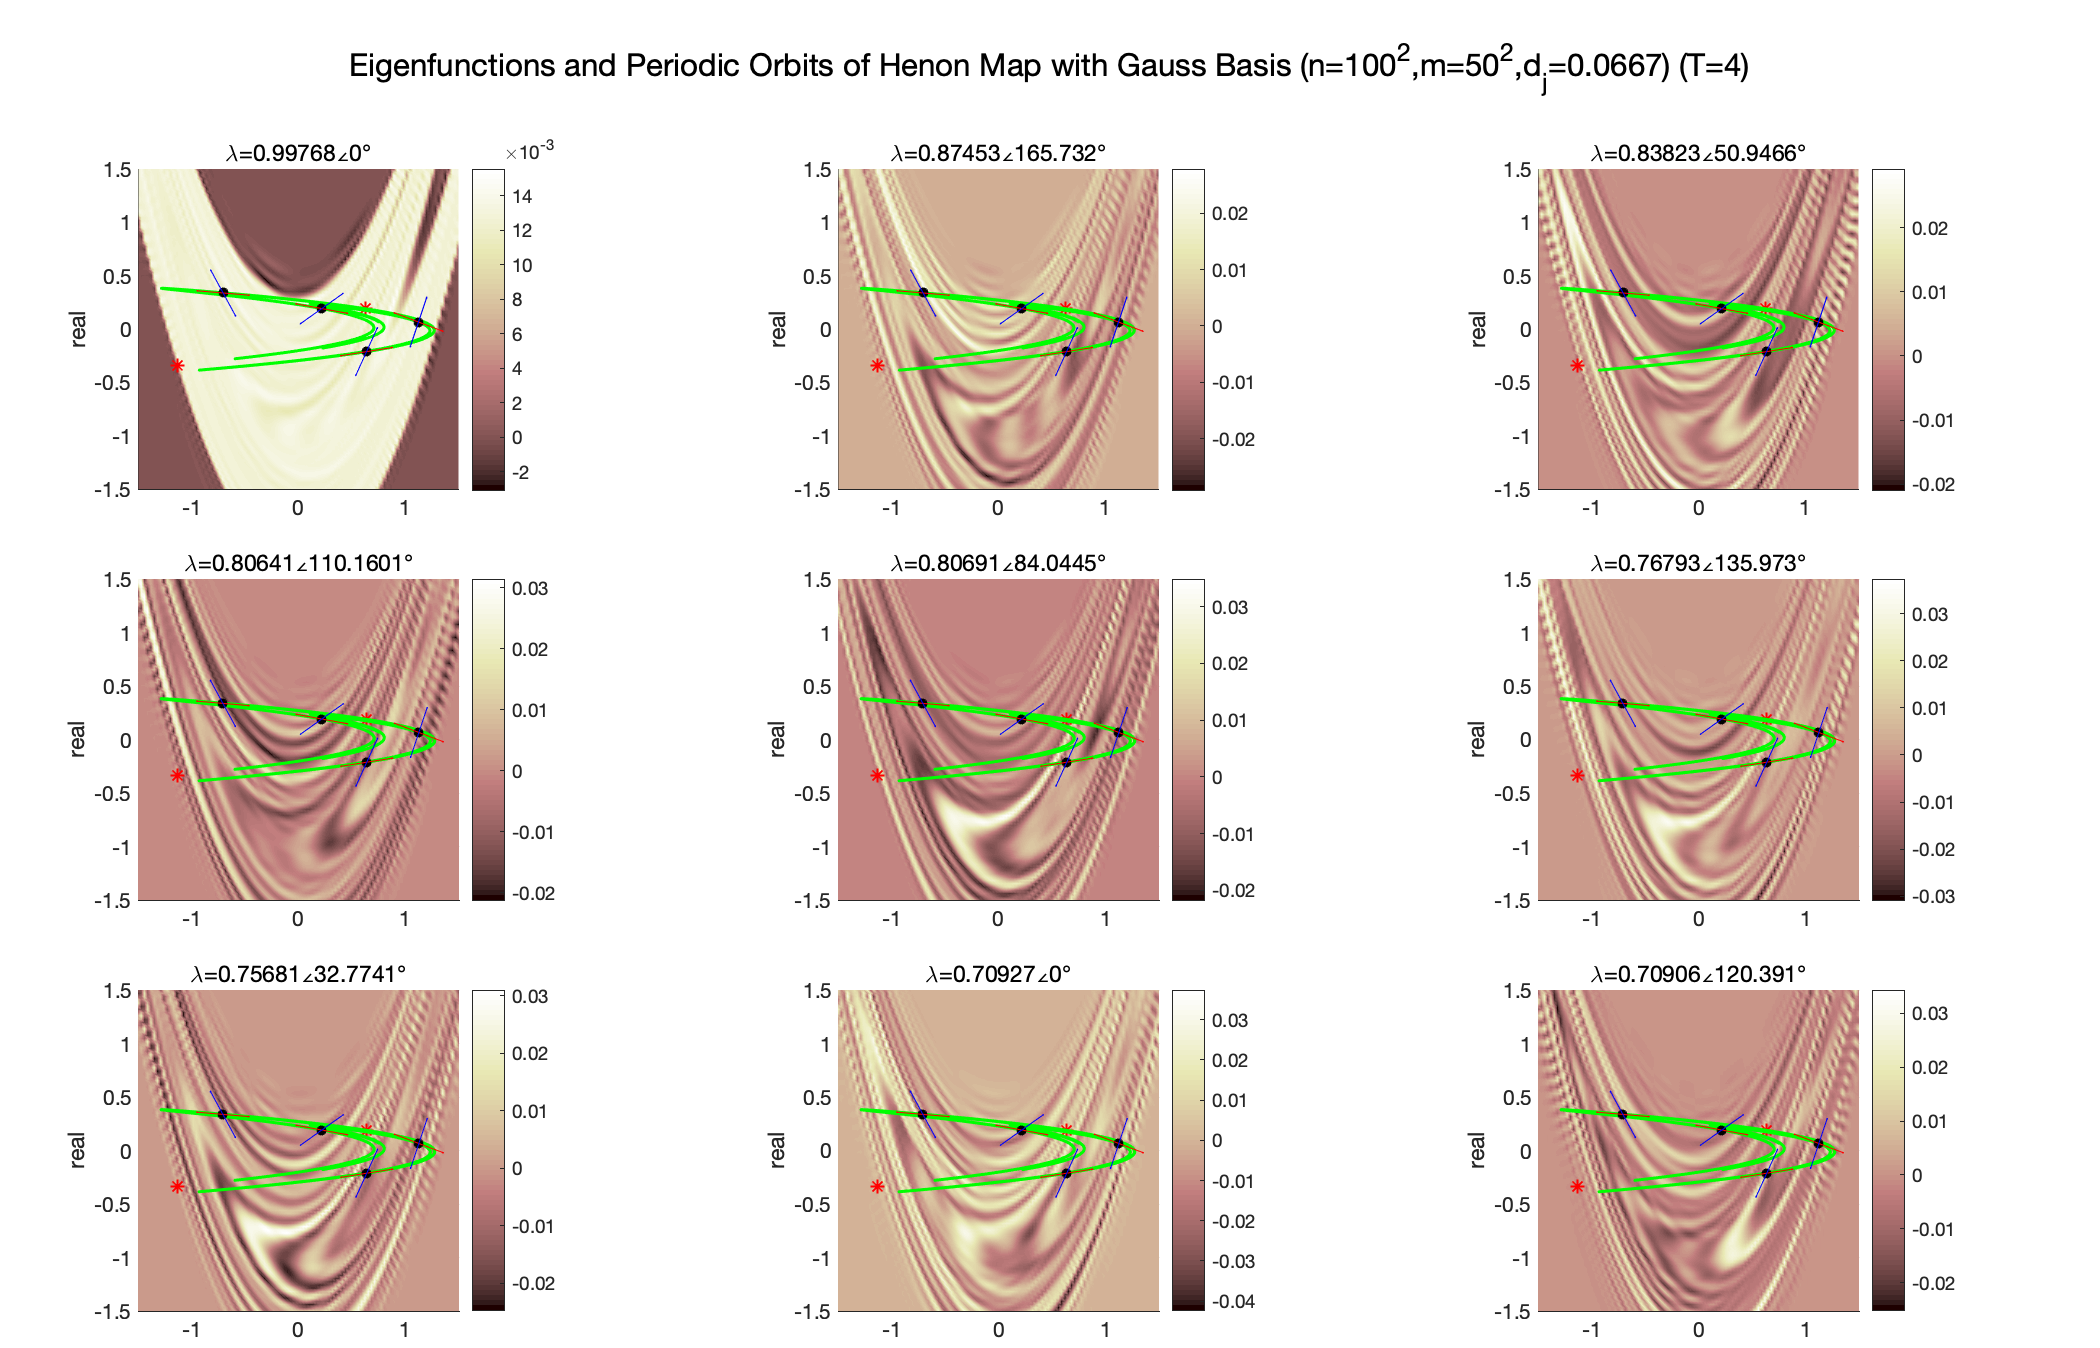
\includegraphics[scale=0.2]{henon/period/Henon_eigen_Gauss_period_n100m50T4}}
    \\
    \subfloat[T=6]{
      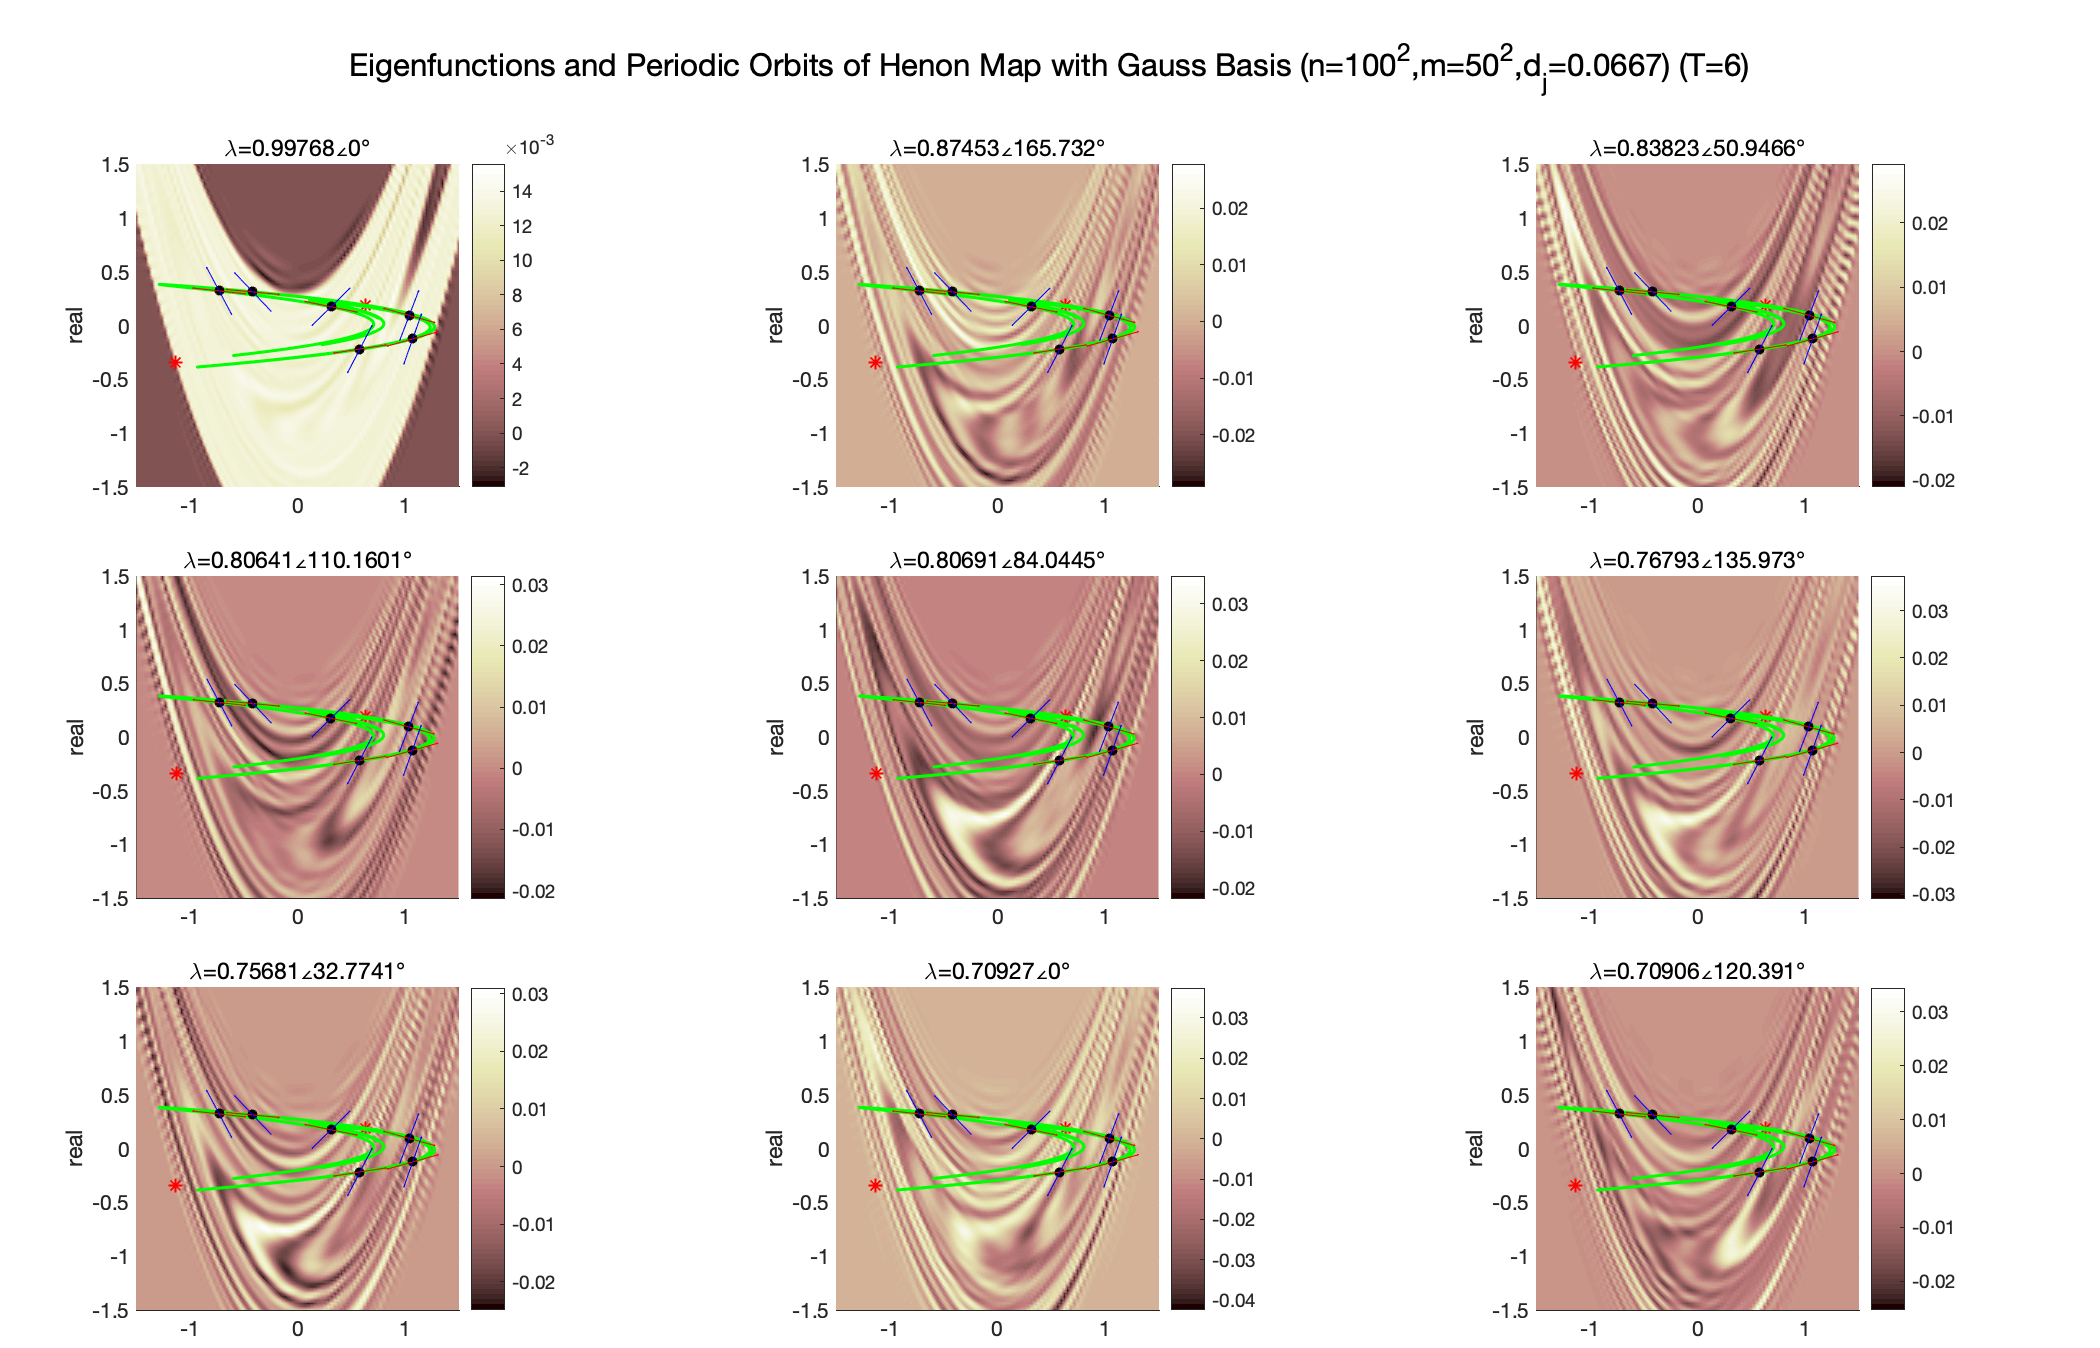
\includegraphics[scale=0.2]{henon/period/Henon_eigen_Gauss_period_n100m50T6}}
    \subfloat[T=7]{
      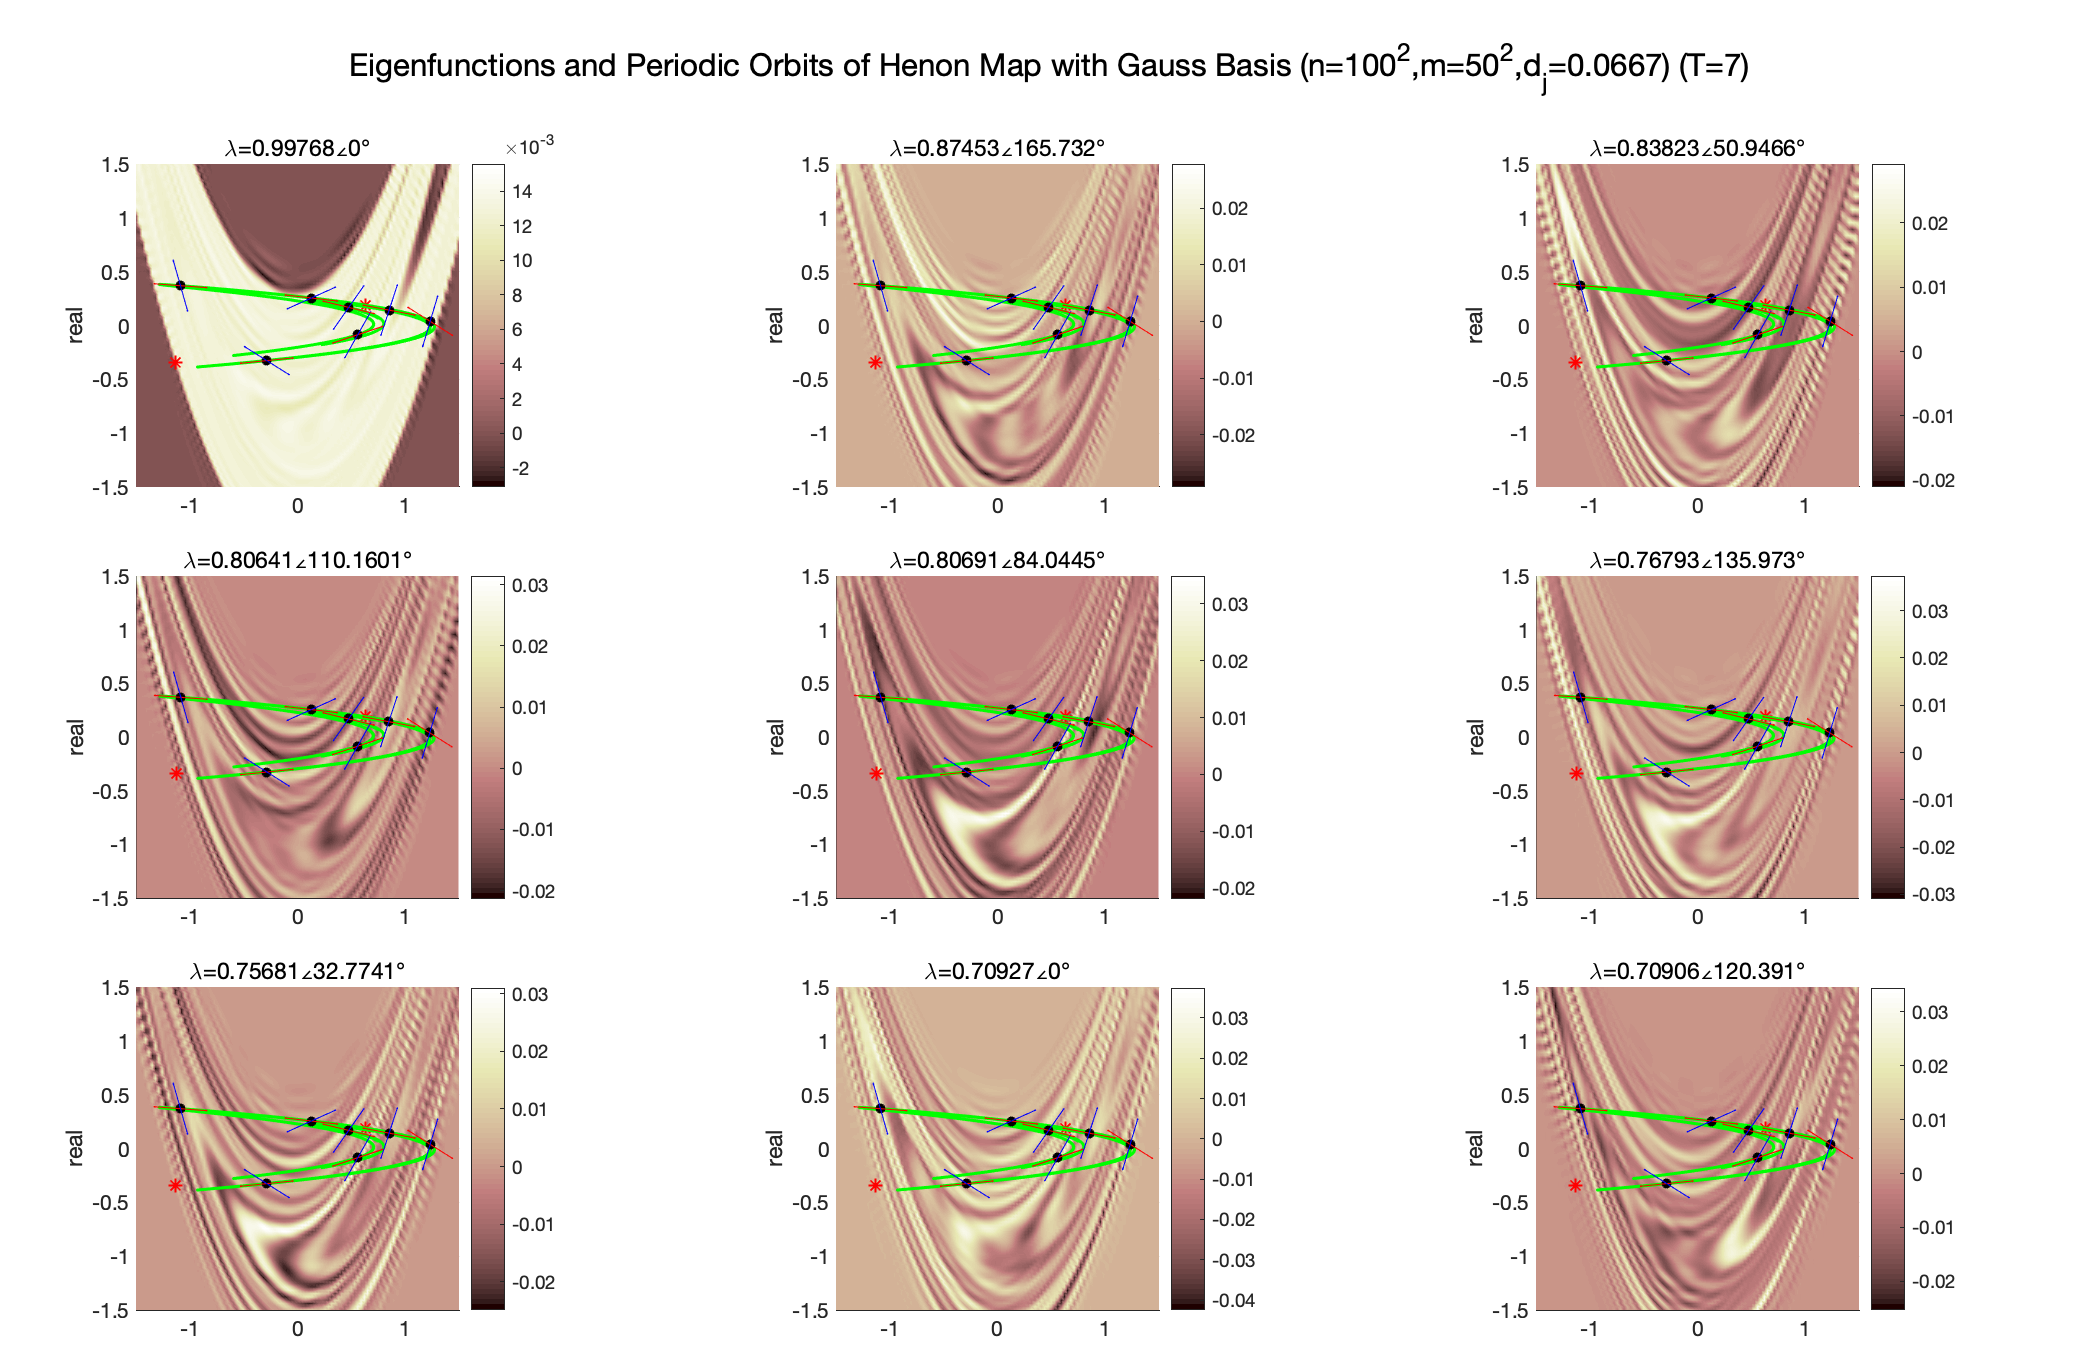
\includegraphics[scale=0.2]{henon/period/Henon_eigen_Gauss_period_n100m50T7}}
    \\
    \caption[埃农映射的本征函数与周期轨道]{埃农映射的本征函数与周期轨道($n=100^2$,$m=50^2,d_j=\frac{3}{45}$):粉色区域表示本征函数值的大小,绿色的线表示吸引子域,黑色的点表示某周期下埃农映射的周期轨道,且每个周期点上存在两个本征方向用箭头表示,蓝色表示不稳定方向,红色表示稳定方向。}\label{fig:Henon_eigen_Gauss_period_n100m50T7}
\end{figure}
我们同样选取$T=12$时周期轨道与本征函数的对比,并将其放大观察,如图\ref{fig:Henon_eigen_Gauss_period1_n100m50T12}。
\begin{figure}
	\centering
	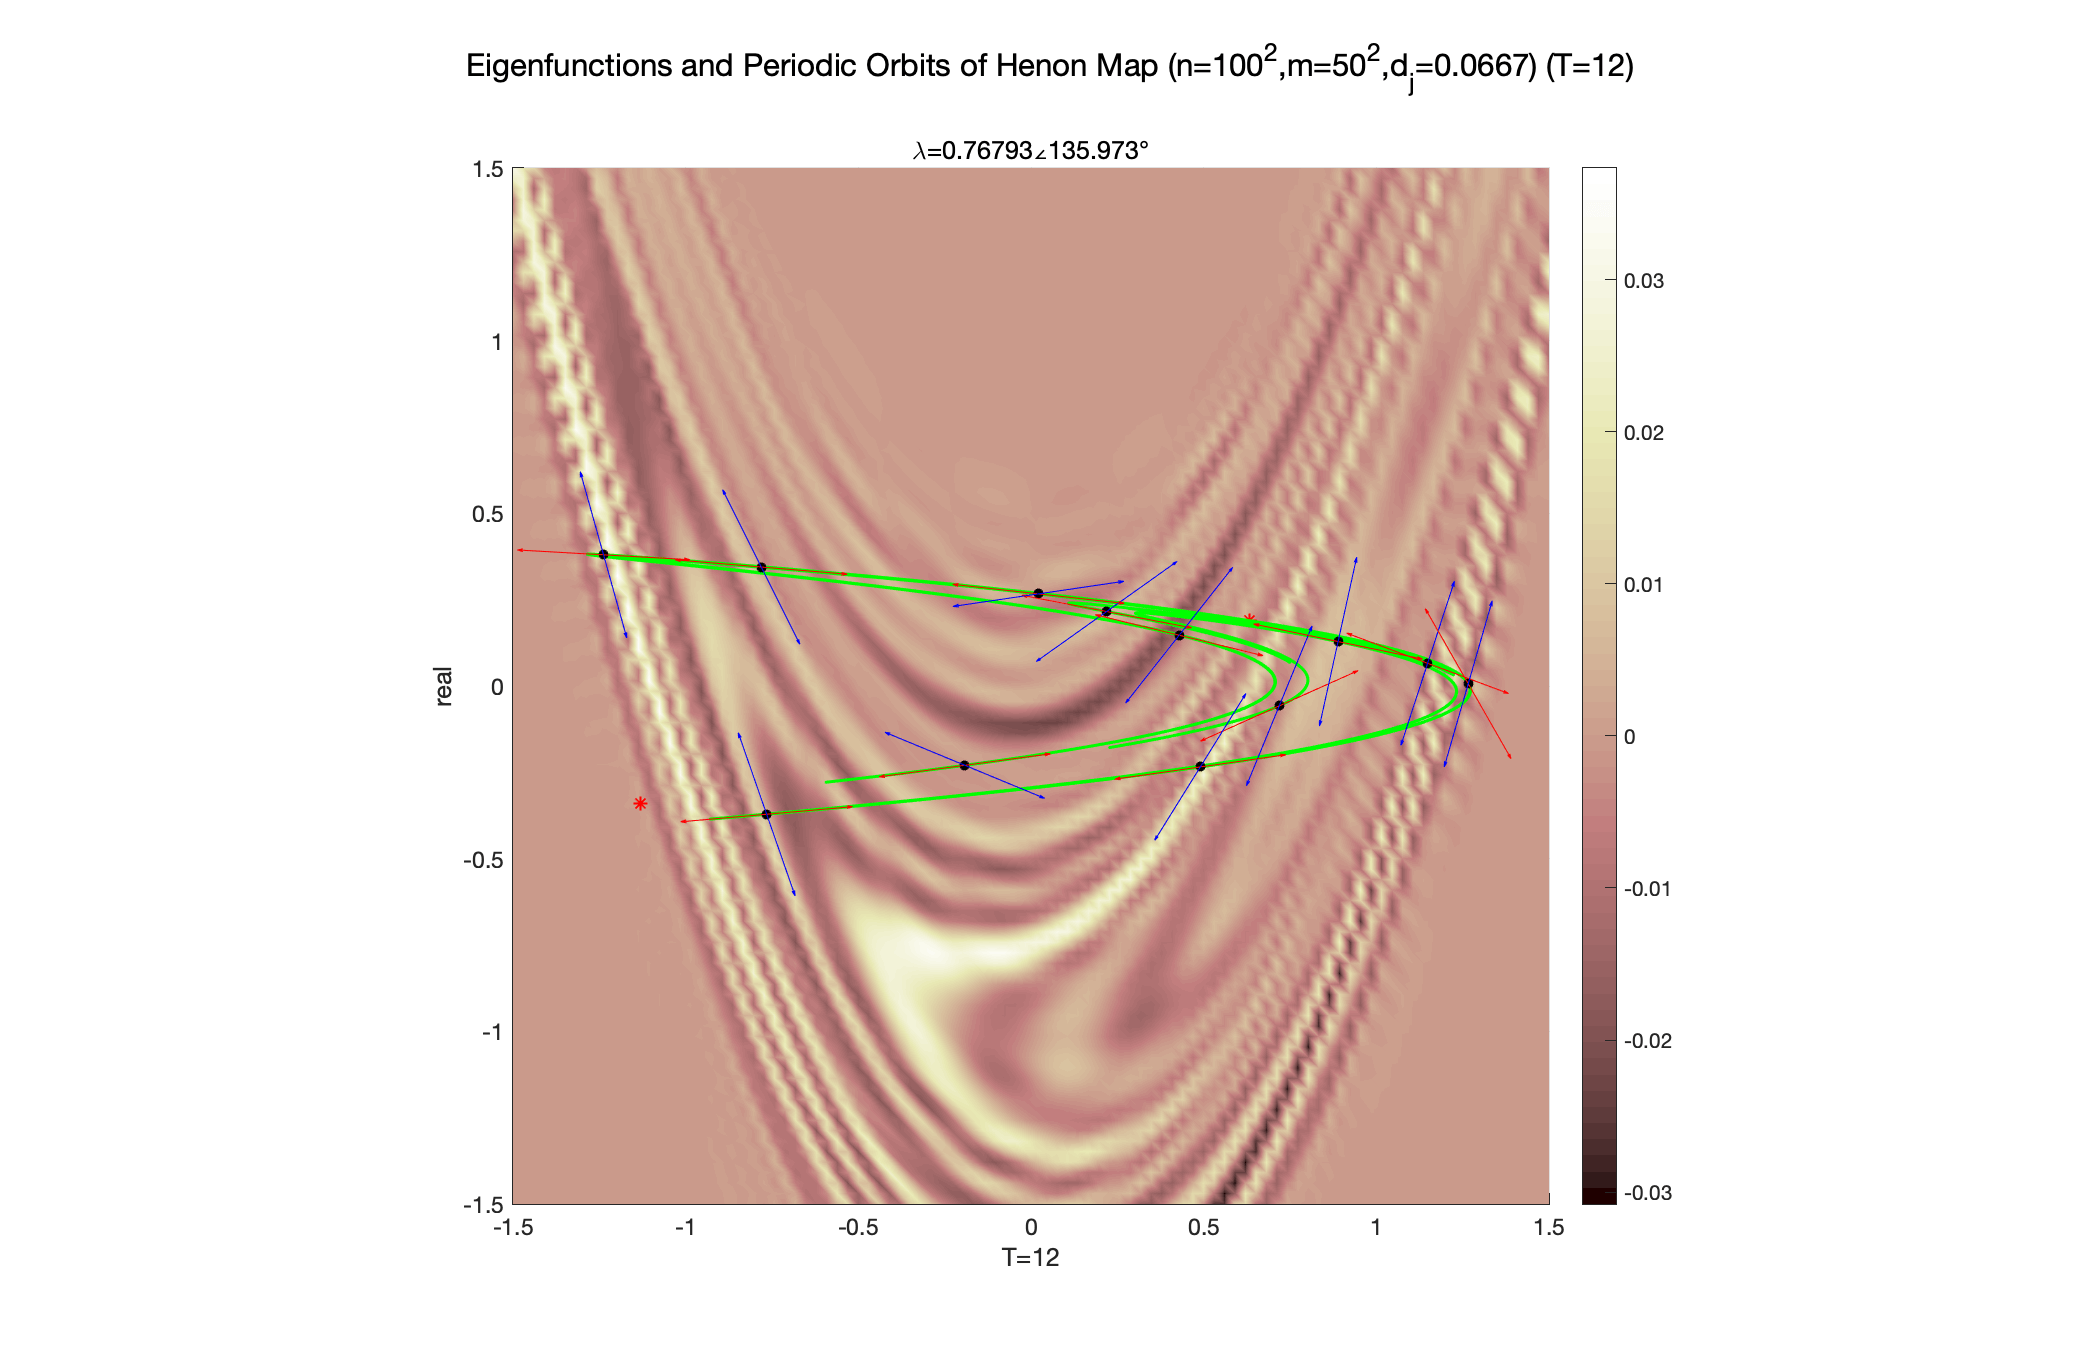
\includegraphics[scale=0.4]{henon/period/Henon_eigen_Gauss_period1_n100m50T12}
    \caption[埃农映射的本征函数与周期轨道]{埃农映射的本征函数与周期轨道(T=12):粉色区域表示本征函数值的大小,绿色的线表示吸引子域,黑色的点表示某周期下埃农映射的周期轨道,且每个周期点上存在两个本征方向用箭头表示,蓝色表示不稳定方向,红色表示稳定方向。}\label{fig:Henon_eigen_Gauss_period1_n100m50T12}
\end{figure}
结合图\ref{fig:Henon_eigen_Gauss_period_n100m50T7}与图\ref{fig:Henon_eigen_Gauss_period1_n100m50T12}我们发现,周期轨道分布在吸引子域上,且其存在两个本征方向,一个方向是稳定的,另一个方向是不稳定的,且稳定的方向即沿着吸引子方向,不稳定的方向沿着埃农映射的本征函数流向,于是我们可以猜测,在相空间$[-1.5,1.5]\times [-1.5,1.5]$中,埃农映射的本征函数图像的流向与埃农映射的不稳定流型一致。

\subsubsection{埃农映射的不稳定流型}
在上一节中,我们得出了一个猜测:埃农映射的本征函数图像的流向与埃农映射的不稳定流型一致,Biham等人于1989年就讨论了H\'{e}non映射的不稳定流型\cite{biham1989characterization}。我们将在此节对其与本征函数的关系作进一步的探究。

我们可以通过数值计算得出埃农映射的不稳定流型:在数值计算中,我们可以先将埃农映射迭代$n$次,再讲埃农映射迭代$-n$(负数表示反向迭代),理论上这样点的位置不会发生变化,但是由于数值计算误差,若初始点不处于不稳定流型,则正向迭代会使其发散,且放大数值计算造成的误差(即使误差很小),这样,粒子再反向迭代回来之后,便很难回到原来的位置。若初始点处于不稳定流型区域中,正向迭代会使其趋于流向吸引子域而非发散,这样反向迭代便可以回到其原来的位置,我们可以利用这样的数据计算技巧确定埃农映射的不稳定流型区域,如图\ref{fig:Henon_iter_reverse_forward},我们取遍布整个相空间的初始点,并画出了当反复迭代次数为$2,5,8,11,14,17,20,23,26$时埃农映射的迭代图。从图中我们可以看到,随着迭代次数的增加,原来处于整个相空间区域的点只剩下了一部分,而这剩下的一部分恰好就反映了不稳定流型的区域。

\begin{figure}
	\centering
	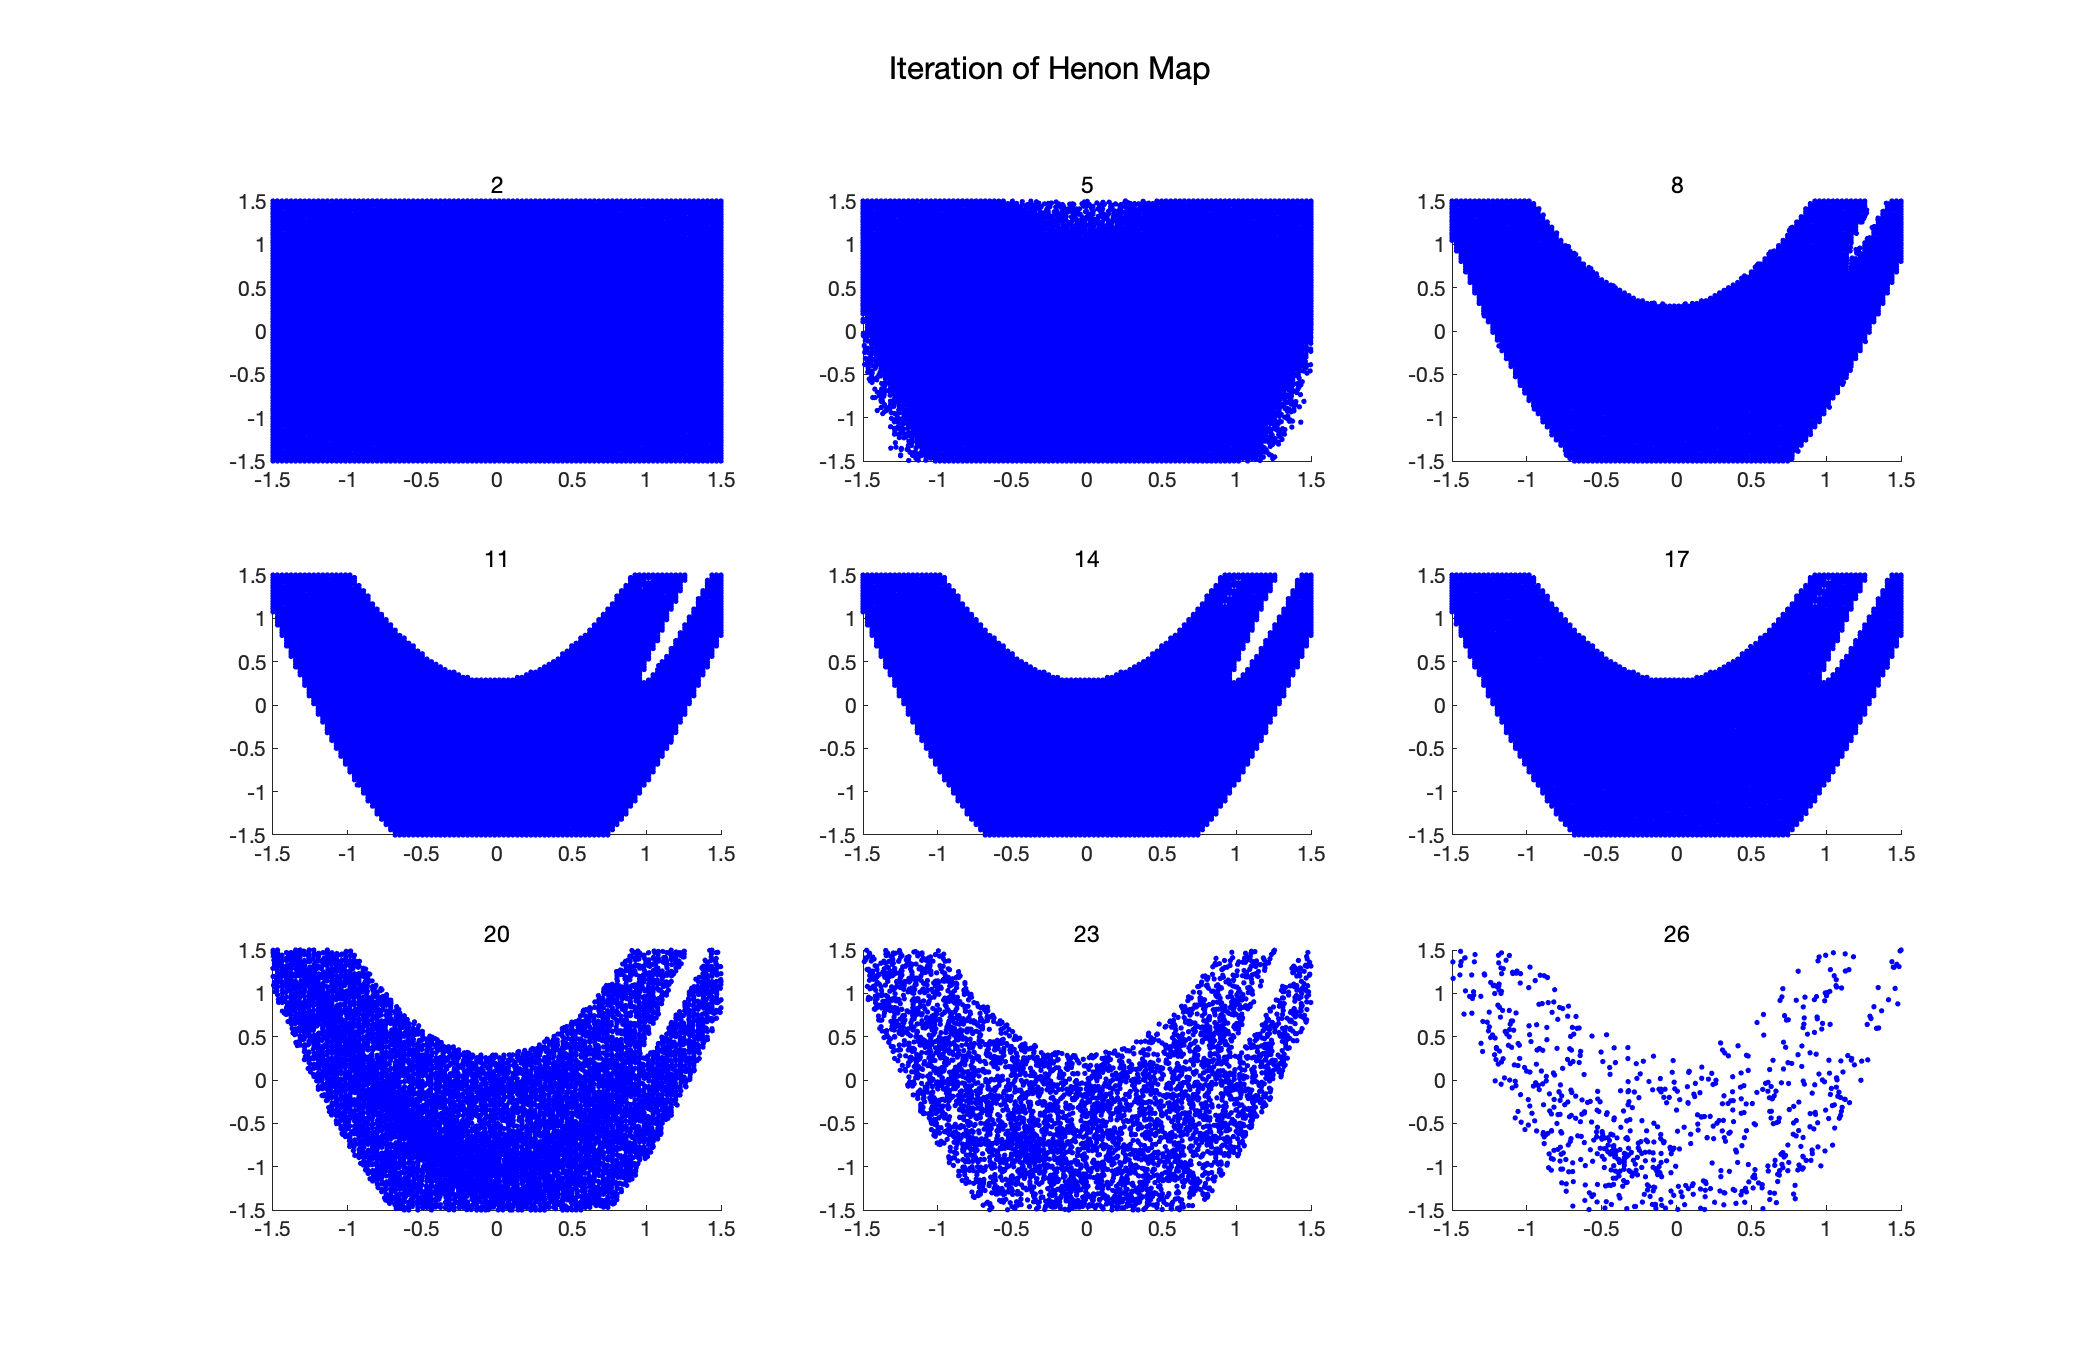
\includegraphics[scale=0.4]{henon/manifold/Henon_iter_reverse_forward}
    \caption{埃农映射的迭代}\label{fig:Henon_iter_reverse_forward}
\end{figure}
我们取迭代次数为20下的不稳定流型区域,并将其与某一个本征函数作对比,如图\ref{fig:Henon_eigen_Gauss_manifold_n100m50}。我们发现,本征函数有明显变化的区域与我们通过迭代寻找到的不稳定流型的区域吻合,这说明了我们得到的本征函数图像的流向恰好就是埃农映射的不稳定流型。
\begin{figure}
	\centering
	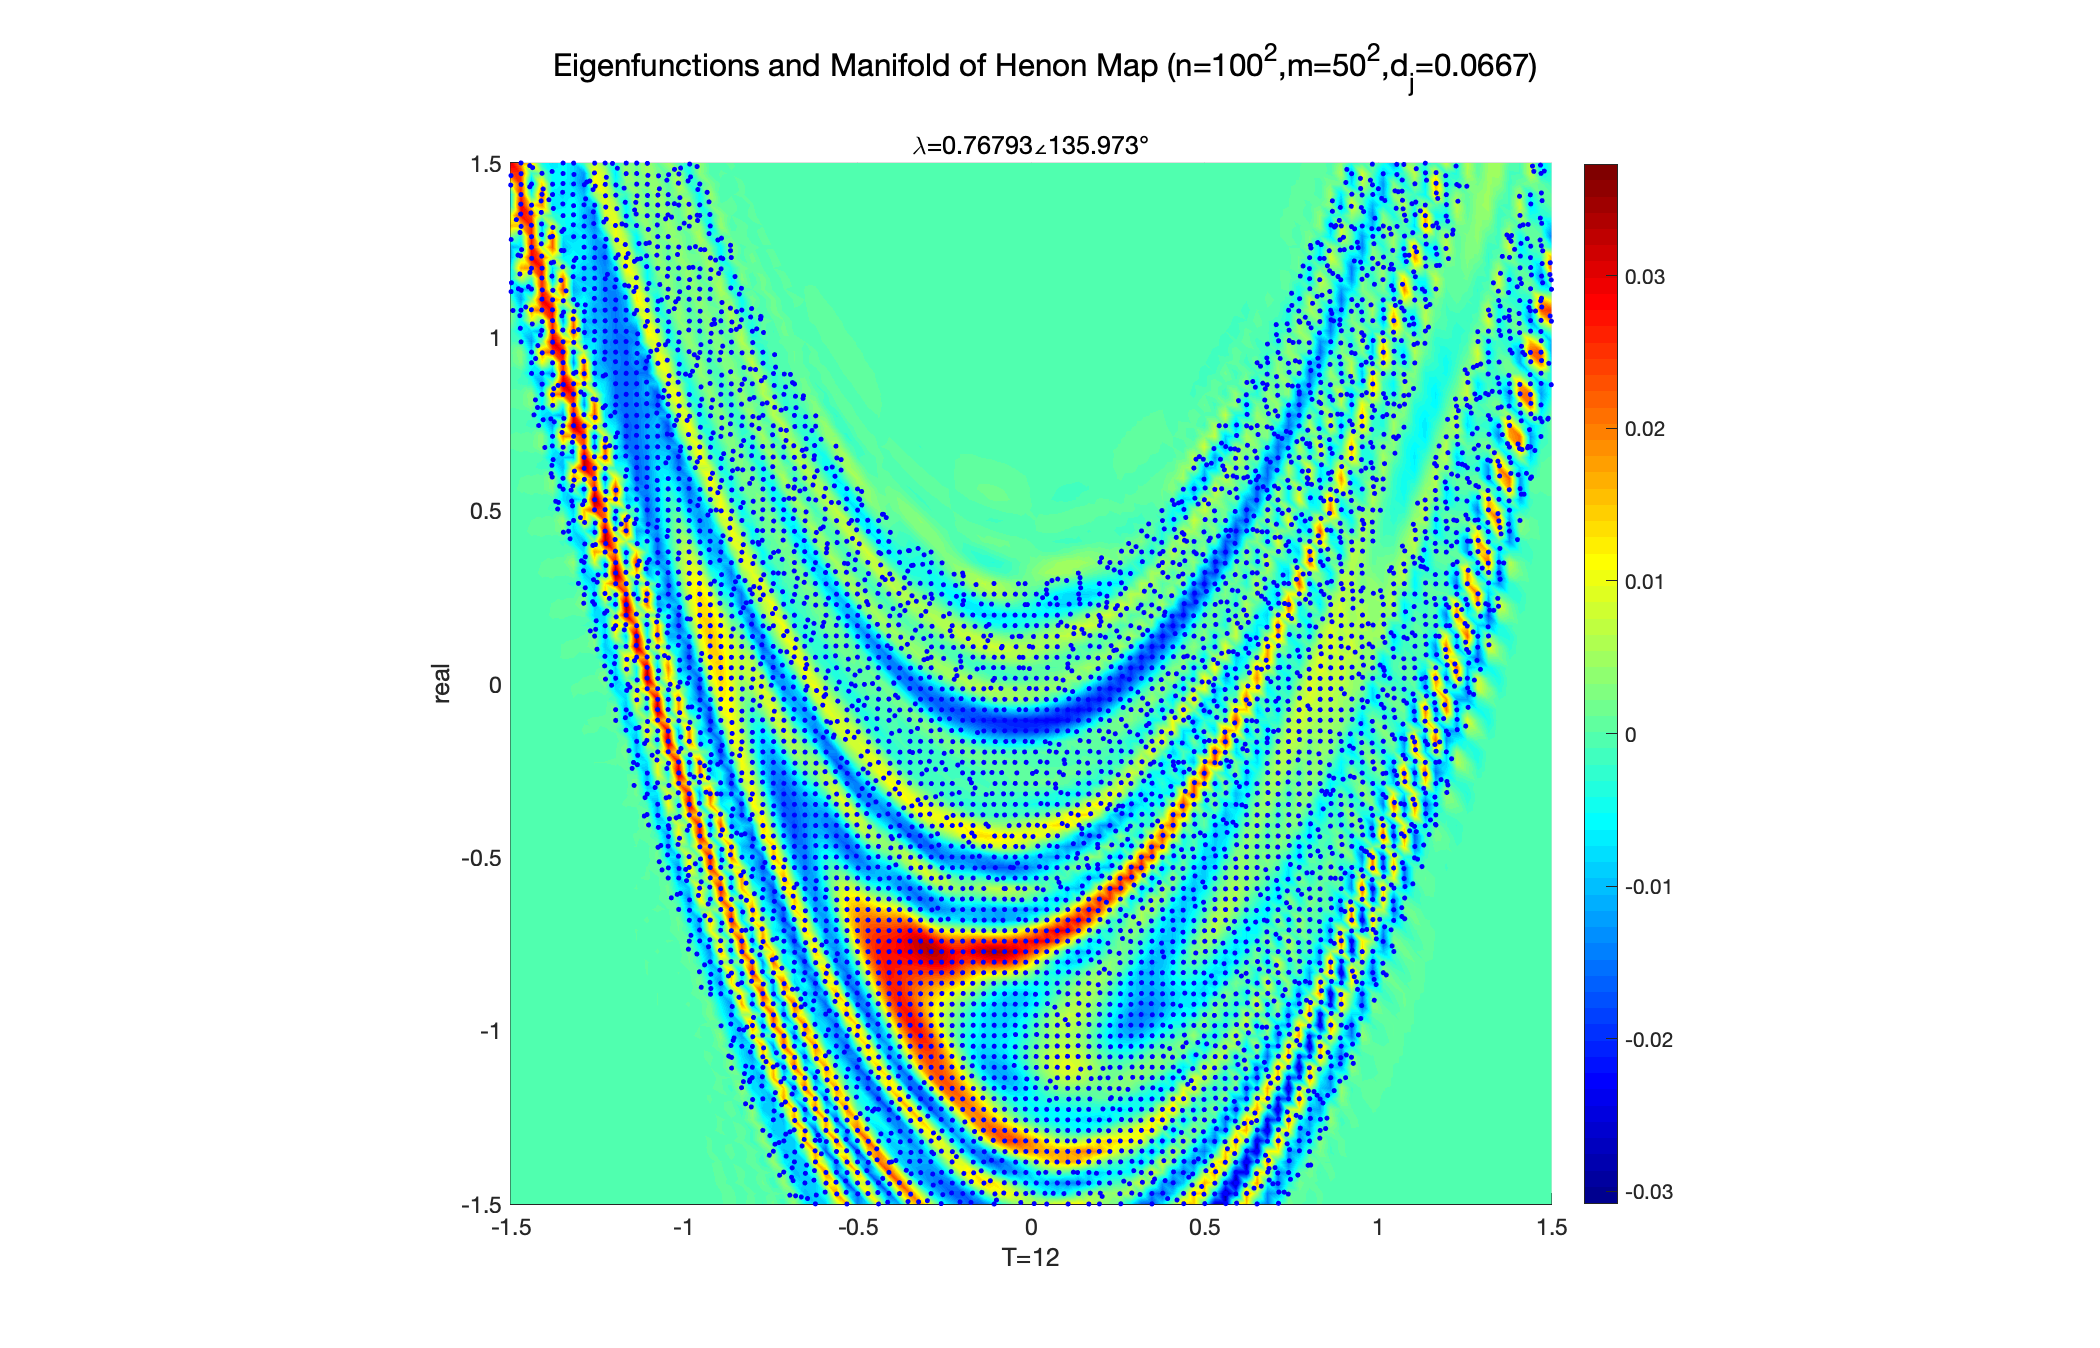
\includegraphics[scale=0.4]{henon/manifold/Henon_eigen_Gauss_manifold_n100m50}
    \caption{埃农映射的迭代与本征函数}\label{fig:Henon_eigen_Gauss_manifold_n100m50}
\end{figure}
为了进一步印证我们的猜想,我们可以较严格的画出埃农映射的不稳定流型。具体方法为,从周期点出发,根据其线性化方向,对其临近的点进行演化,若我们演化的间隔足够小,我们便可以通过将这些轨迹连接起来得到埃农映射的不稳定流型。为了使我们演化的间隔比较均匀,Hobson提出了一种演化不稳定流型的计算方法,我们利用这种方法,画处$T=4$时,由周期轨道演化而成的埃农映射的不稳定流型,如图\ref{fig:Henon_eigen_Gauss_manifold_n100m50T4}。
\begin{figure}
	\centering
	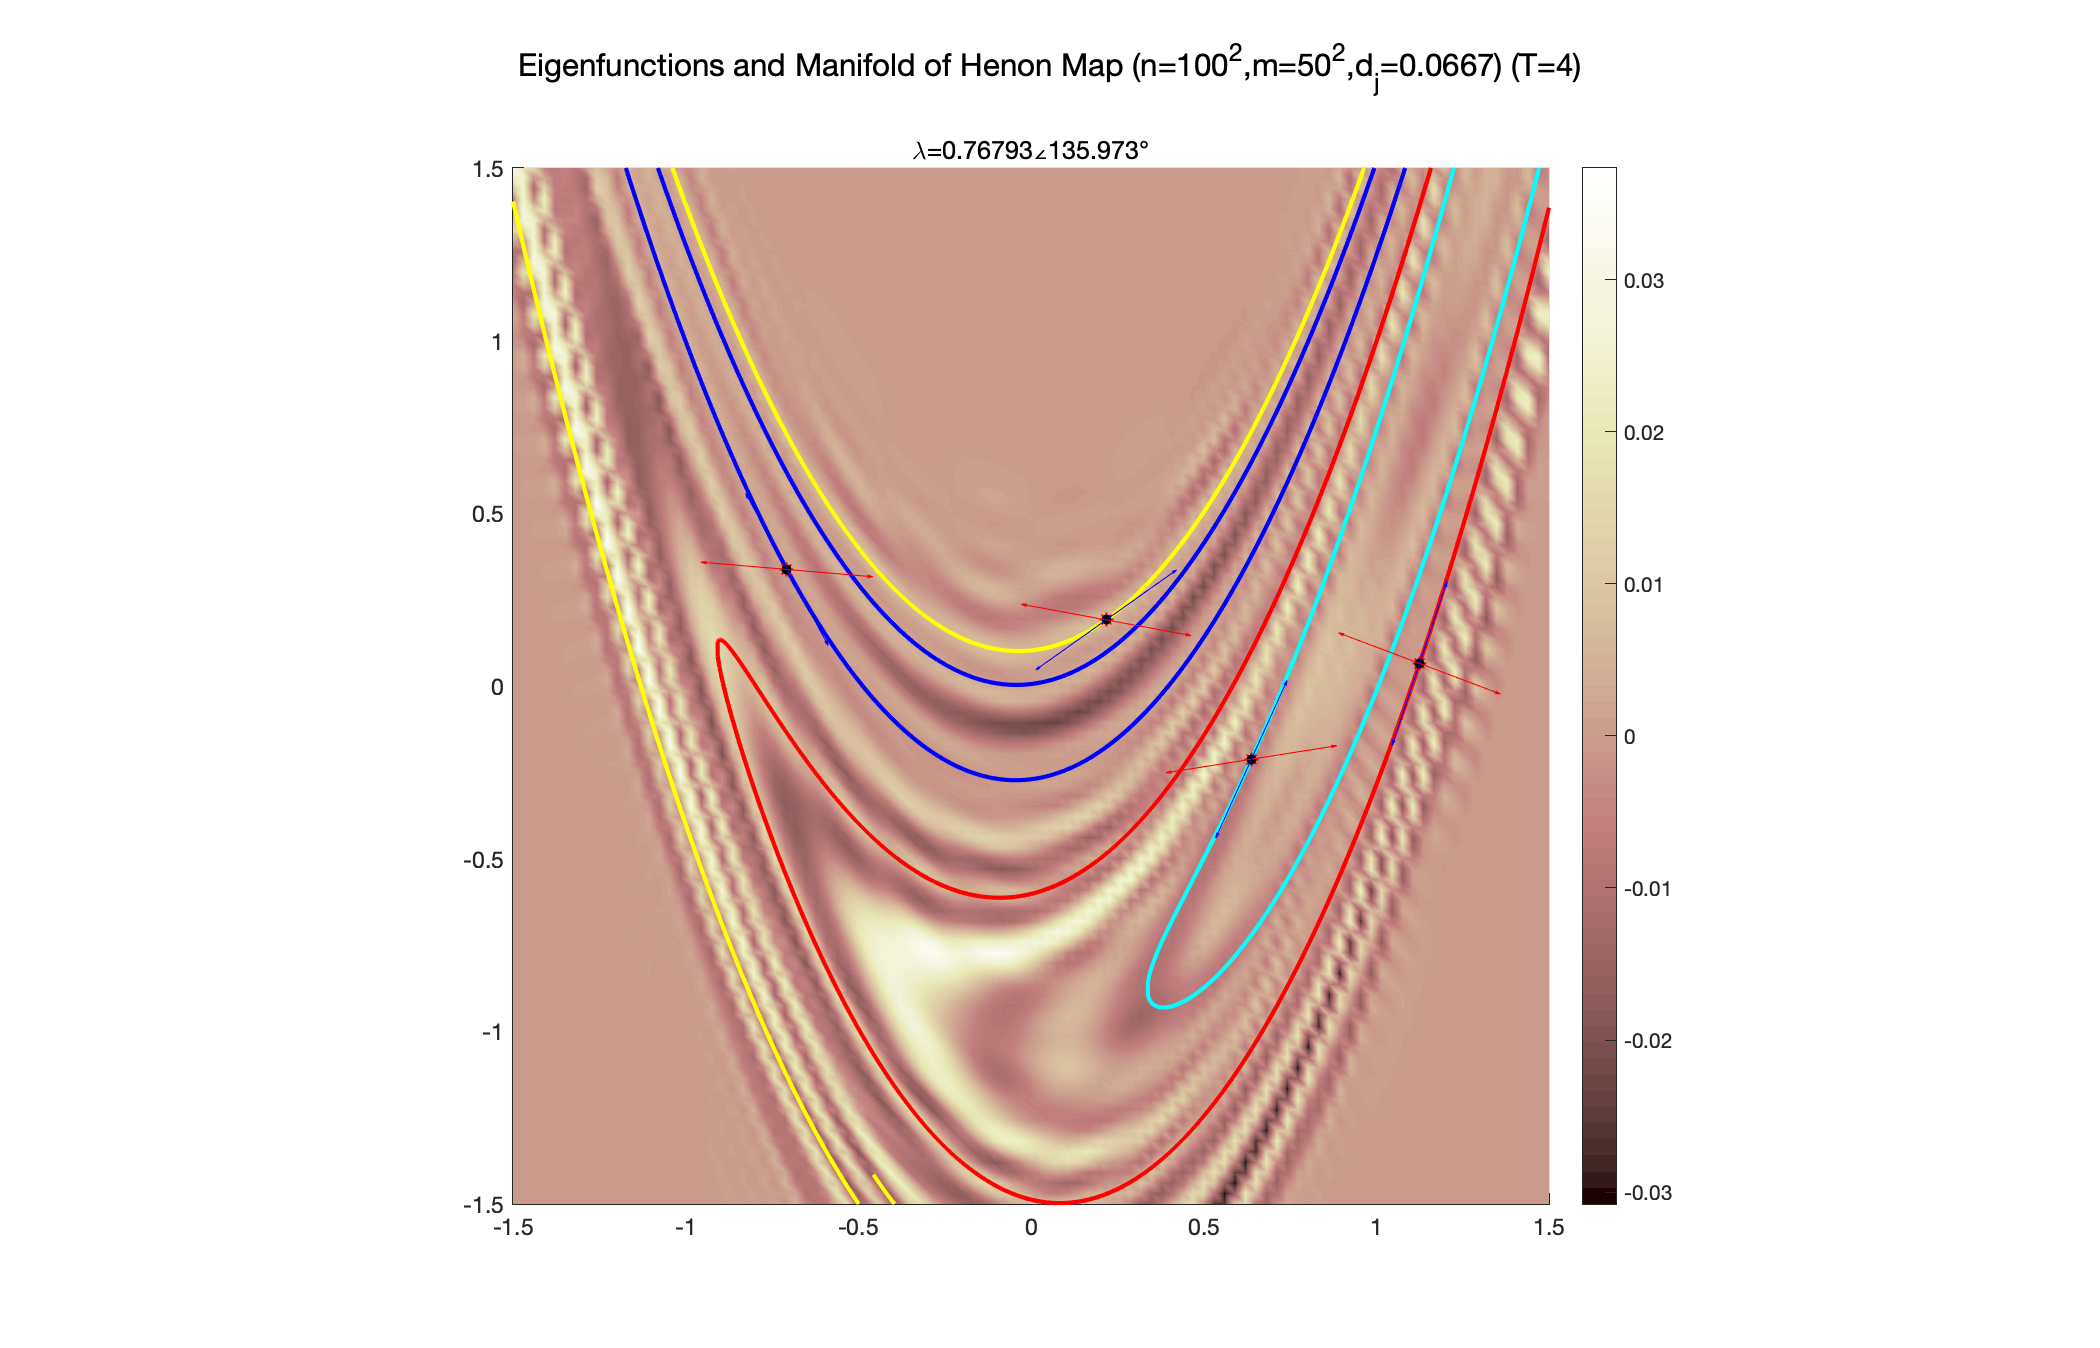
\includegraphics[scale=0.4]{henon/manifold/Henon_eigen_Gauss_manifold_n100m50T4}
    \caption[埃农映射的不稳定流型与本征函数]{埃农映射的不稳定流型与本征函数(T=4):粉色区域表示埃农映射的本征函数,黑色的点表示周期4轨道的位置,两个本征方向用蓝色与红色箭头标出,沿着不稳定方向(蓝色)演化而成的不稳定流型用实线标出,且四个点演化而成的不稳定流型轨道颜色不同}\label{fig:Henon_eigen_Gauss_manifold_n100m50T4}
\end{figure}
当周期$T=7$时,我们可以计算得到四组不同的周期轨道,我们分别计算这四组轨道下演化而成的埃农映射的不稳定流型,并将其与本征函数作为对比,如图\ref{fig:Henon_eigen_Gauss_manifold_n100m50T7_4}。
\begin{figure}
    \centering
    \subfloat{
      \includegraphics[scale=0.2]{henon/manifold/Henon_eigen_Gauss_manifold_n100m50T7_1}}
    \subfloat{
      \includegraphics[scale=0.2]{henon/manifold/Henon_eigen_Gauss_manifold_n100m50T7_2}}
    \\
    \subfloat{
      \includegraphics[scale=0.2]{henon/manifold/Henon_eigen_Gauss_manifold_n100m50T7_3}}
    \subfloat{
      \includegraphics[scale=0.2]{henon/manifold/Henon_eigen_Gauss_manifold_n100m50T7_4}}
    \\
    \caption[埃农映射的不稳定流型与本征函数]{埃农映射的不稳定流型与本征函数(T=7):粉色区域表示埃农映射的本征函数,黑色的点表示周期4轨道的位置,两个本征方向用蓝色与红色箭头标出,沿着不稳定方向(蓝色)演化而成的不稳定流型用实线标出,且四个点演化而成的不稳定流型轨道颜色不同}\label{fig:Henon_eigen_Gauss_manifold_n100m50T7_4}
\end{figure}
结合图\ref{fig:Henon_eigen_Gauss_manifold_n100m50T4}与图\ref{fig:Henon_eigen_Gauss_manifold_n100m50T7_4}。我们发现,周期轨道迭代下产生的不稳定流型与埃农映射的本征函数流向一致,且在一条不稳定流型轨道上,本征函数值的大小几乎一致。于是我们可以验证我们的猜测:在埃农映射中,Koopman算符的本征函数流向与不稳定流型一致。同时我们可以观察到,在同一条不稳定流型轨道中,本征函数值的大小几乎相同。

%\subsection{小结}